\documentclass[11pt]{article}
\usepackage{amsmath,amssymb,amsthm,mathtools}
\usepackage{geometry,booktabs,array,multirow,enumitem,longtable}
\usepackage{graphicx,xcolor}
\usepackage{placeins}
\usepackage[colorlinks=true,linkcolor=black,citecolor=black,urlcolor=blue]{hyperref}
\geometry{margin=2.2cm}
\emergencystretch=3em
\graphicspath{{figures/}}
\DeclarePairedDelimiter{\abs}{\lvert}{\rvert}
\DeclarePairedDelimiter{\norm}{\lVert}{\rVert}
\newcommand{\R}{\mathbb R}
\newcommand{\W}{W}
\newcommand{\Lop}{\mathcal L}
\newcommand{\Erem}{\mathcal E}
\newcommand{\wt}[1]{\widetilde{#1}}
\newcommand{\dd}{\,\mathrm d}
\DeclareMathOperator{\diag}{diag}
\DeclareMathOperator{\tr}{tr}
\DeclareMathOperator{\spanop}{span}
\DeclareMathOperator{\TV}{TV}
\DeclareMathOperator{\sech}{sech}
\newtheorem{assumption}{Assumption}[section]
\newtheorem{definition}{Definition}[section]
\newtheorem{lemma}{Lemma}[section]
\newtheorem{proposition}{Proposition}[section]
\newtheorem{theorem}{Theorem}[section]
\newtheorem{corollary}{Corollary}[section]
\newtheorem{example}{Example}[section]
\newtheorem*{remark}{Remark}
\numberwithin{equation}{section}
\newcommand{\expclaim}[1]{\textcolor{teal!60!black}{[empirical~$n={#1}$]}}

\title{\textbf{What Spatial Weighting Can and Cannot Change in PINNs:\\Spectral Capability Bounds of Local Diagonal Weights with Controlled Falsification}\\[3pt]
\large --- Solution-Set Invariance, Conditioning Bounds, and Basin-Selection Tests in Viscous Burgers Shock Capturing}
\author{Ning Wen\\[2pt]
\small Independent Researcher\\[1pt]
\small \href{mailto:wenning-compmath@outlook.com}{wenning-compmath@outlook.com}\\[1pt]
\small \href{https://orcid.org/0009-0005-5395-7791}{ORCID: 0009-0005-5395-7791}}
\date{}

\begin{document}
\maketitle
\begin{abstract}

Physics-informed neural networks (PINNs) often converge to wrong (pseudo-)solutions on stiff problems, and spatial weighting is one of the most common interventions. This paper revolves around one question: for the weighted training objective $L_\W=\tfrac{1}{2N} r^\top \W r$ (empirical-mean convention, frozen or exogenous slowly-varying weights), which mathematical objects does changing the spatial diagonal weight $\W$ actually act on, and what is the causal chain in each case? To organize the analysis, we separate the effects of weighting by Taylor-expansion order into a zeroth-order level (solution set/well-posedness), a first-order level (gradient/optimization dynamics), and a second-order level (frozen linearization spectrum).

We establish three classes of capability boundaries. (1)~At the second-order level, spatially local diagonal weighting leaves the correlation matrix of the frozen Gram matrix exactly invariant and can only rescale the eigenvalue scales within a bounded band (the van der Sluis band); on equicorrelation matrices the condition number is already optimal. The only whitening weight, the non-local $\W\propto K_r^{-1}$, is dense and costs $O(N^3)$, making online training infeasible. Experiment 4.2 verifies this strictly and statically on a real frozen Burgers Jacobian: the improvement \emph{found} by multi-start L-BFGS-B is 13\%--24\% for $N\le512$; at $N=1024$, $\kappa(R)\gtrsim10^{13}$ is near the double-precision limit and is excluded from quantitative conclusions; the true optimal improvement is no smaller than these values (optimized values are upper bounds), and the improvement ceiling is constrained by the van der Sluis band $r\ge1/N$. That whitening is impossible is algebraically guaranteed by the theorem. Experiment 4.3 serves as an in-training empirical corroboration. Under the default clipping configuration, the down-weighting families worsen conditioning by $1.7$--$4.9\times$, and by $3.0$--$4.9\times$ at the low viscosities $.001$/.005; with clipping off, the range is wider ($0.6$--$3.4$) and individual cells show improvement. This experiment measures the full Hessian, not the frozen $H_{\rm lin}$.

(2)~At the first-order level, across the six weight families studied here with $n=80$ paired experiments, we do not observe that weighting significantly improves the basin-entry probability (the uniform hit rate $.613$ is in fact higher than that of all weighted families; after Holm correction only down\_lin is significant, $p=.006$); the observable effect of weighting is confined to modulating the convergence speed inside an already-entered basin. Down-weighting acts mainly as gradient-scale modulation (the residual directional effect after Adam normalization is small: Experiment 5.8 finds that down\_lin raises the effective lr ceiling by a factor of two, with exact two-sided $p=.0625$ (asymptotic $\approx.043$), a consistent direction that does not reach $.05$ significance): when scale is not the bottleneck it only stabilizes early training, while under spectral mismatch it can bring terminal-state benefits (cross-equation verification). The post-hoc optimal $\beta$ is a descriptive observation (per-seed spread $1$--$100$), not a fixed strategy deployable before training.

(3)~When no ground truth is available at deployment, basin discrimination by a fixed single-projection scalar (residual/loss self-evaluation) is limited by a Bayes error lower bound; a four-point XOR counterexample shows exact linear separation is impossible (minimum error $1/4$), so interaction/nonlinear features are necessary. The quantity $g_{et}$, which carries spatial-contrast structure, provides feasibility evidence for basin discrimination (proxy AUC $.971$, with label--feature common-source correlation; oracle AUC $.64$); it is a noisy discriminator whose value lies in filtering out obviously bad basins and reducing wasted refinement, not in precisely identifying good basins. The main testbed is the one-dimensional steady viscous Burgers shock, with a smooth Poisson degeneracy and internal-singularity prototypes as cross-equation verification. All conclusions are labeled at one of three statement levels: certain, with probability $1-\delta$, or empirical $n=$.

\end{abstract}

\noindent\textbf{Keywords:} physics-informed neural networks (PINNs); spatial weighting; condition number; correlation-matrix invariance; basin of attraction; viscous Burgers equation; pseudo-solutions


\section{Introduction}\label{sec:intro}

\subsection{Background and Problem}\label{sec:bg}
Physics-informed neural networks (PINNs) incorporate PDE residuals and initial/boundary conditions as soft constraints in the loss function and approximate the solution with a fully connected network; they are widely used in both forward and inverse problems \cite{Raissi2019,Karniadakis2021,Cuomo2022}. When the solution is smooth and the operator well-conditioned, the method is robust; but on \emph{stiff} problems---convection-dominated regimes, thin boundary layers, or shocks---PINNs often exhibit stalled training loss, convergence to physically wrong pseudo-solutions, or high sensitivity to initialization. Existing studies offer explanations from different angles: stiffness causes gradient-magnitude mismatch among loss terms \cite{WangTeng2020}; in the neural tangent kernel (NTK) view, the convergence rates of different loss components are determined by, and mismatched across, the corresponding kernel eigenvalues \cite{Jacot2018,Wang2020NTK}; improper soft-constraint weights and wrong optimization curvature systematically induce failure modes \cite{Krishnapriyan2021}; and the spectral bias of networks makes them learn low-frequency components first \cite{Rahaman2019,Tancik2020}.

\emph{Spatial weighting}---assigning different weights to residuals according to the spatial location of collocation points---is the most direct and most common intervention against these difficulties. The literature develops along several seemingly contradictory routes: increasing weights in ``hard regions'' where residuals are large (hard-region up-weighting, adaptive collocation (RAR/RAD-type \cite{Wu2022,Nabian2021}, which belongs to the out-of-class adaptive-sampling family), causal training \cite{Wang2022causal}); or, conversely, \emph{de-emphasizing} hard regions---either by down-weighting the loss there or by weakening the network expression \cite{Liu2022down,LessEmphasis2022}; there is also work that resolves gradient conflicts via orthogonal projection \cite{ConFIG2025}. These methods are each effective on their own examples, but they act at different levels. Three kinds of claims are therefore frequently conflated in the literature: (a)~claiming that optimization is improved on the grounds that the zeroth-order solution set is invariant under weighting; (b)~inferring directly from changes in the frozen Hessian/NTK spectrum that training trajectories are improved; (c)~interpreting a drop in gradient magnitude early in training as ``escaping a wrong attraction basin.'' Without conceptually separating these levels, one cannot tell under what conditions a weighting strategy is effective, nor where the boundaries of its benefits and costs lie.

\subsection{The Overarching Question and the Separation of Analysis Levels}\label{sec:q}
The common root of the three confusions above is the lack of a causal localization of what weighting acts on. The overarching question of this paper is therefore: for the weighted training objective $L_{\W}=\tfrac{1}{2N} r^\top \W r$ (empirical-mean convention, $\W$ a spatial diagonal weight), which mathematical objects does changing $\W$ act on, and what is the causal chain in each case? To organize the analysis, we separate these objects into three levels by Taylor-expansion order (Figure~\ref{fig:box}); this separation serves only to organize the analysis and prevent cross-level conclusions from being used as mutual evidence, and does not constitute an independent theoretical contribution. The first is the \emph{zeroth-order level}: the zero-residual solution set, well-posedness, and the residual-to-error stability bridge, none of which changes with $\W$ when $w>0$. The second is the \emph{first-order level}: the weighted gradient field $g_{\W}=J^\top\W r$, the iteration trajectories it induces, and global geometry such as stationary points/attraction basins (a basin of attraction---the set of initial values from which optimization iterates converge to the same stationary point---is simply called a ``basin'' throughout; one converging to a pseudo-solution is a pseudo-solution basin, and one refinable to the true solution is a refinable basin). In a large class of first-order algorithms, the only differential route by which $\W$ enters a \emph{single-step} parameter update is the weighted gradient $g_{\W}$ (line search on the scalar loss $L_\W$ is out of class; see~\ref{sec:admit}). The third is the \emph{second-order level} (frozen linearization spectrum): $H_{\rm lin}=J^\top\W J$ and its spectrum. It is the linearized tangent matrix at the current point and acts only indirectly through multi-step gradient evolution; the indefiniteness of the true Hessian comes from the residual curvature $H_{\rm nl}=\sum_i w_i r_i\nabla_\theta^2 r_i$, which vanishes as the residual tends to zero. $H_{\rm nl}$, third- and higher-order Taylor terms, curvature drift within a training window, preconditioner time-variation, and exogenous jumps are collectively grouped into a \emph{controlled remainder} (a residual bucket with explicit bounds). Along the time dimension, training has two phases: \emph{Phase~0 (basin selection)} enters the correct basin at $\beta=1$ via a representation curriculum and multi-start selection; the \emph{Gate} performs a one-shot policy split without using the ground truth; \emph{Phase~1 (in-basin refinement)} adjusts the up-weighting strength $\beta$ inside an already-entered refinable basin to complete local convergence. Experimentally, the main testbed throughout is the one-dimensional steady viscous Burgers shock, with a smooth Poisson degeneracy, internal-singularity prototypes, one-dimensional time-dependent Burgers, and two-dimensional linear convection--diffusion as cross-equation verification. This separation directly yields testable judgments: for example, ``weighting improves the frozen condition number'' and ``weighting accelerates convergence'' are two different propositions at the second and first order respectively---the former generally fails for spatially local weighting, the latter holds only under specific in-basin conditions, and neither can serve as evidence for the other. Section~\ref{sec:framework} gives the strict formalization of the notation and definitions above.

\begin{figure}[ht]\centering
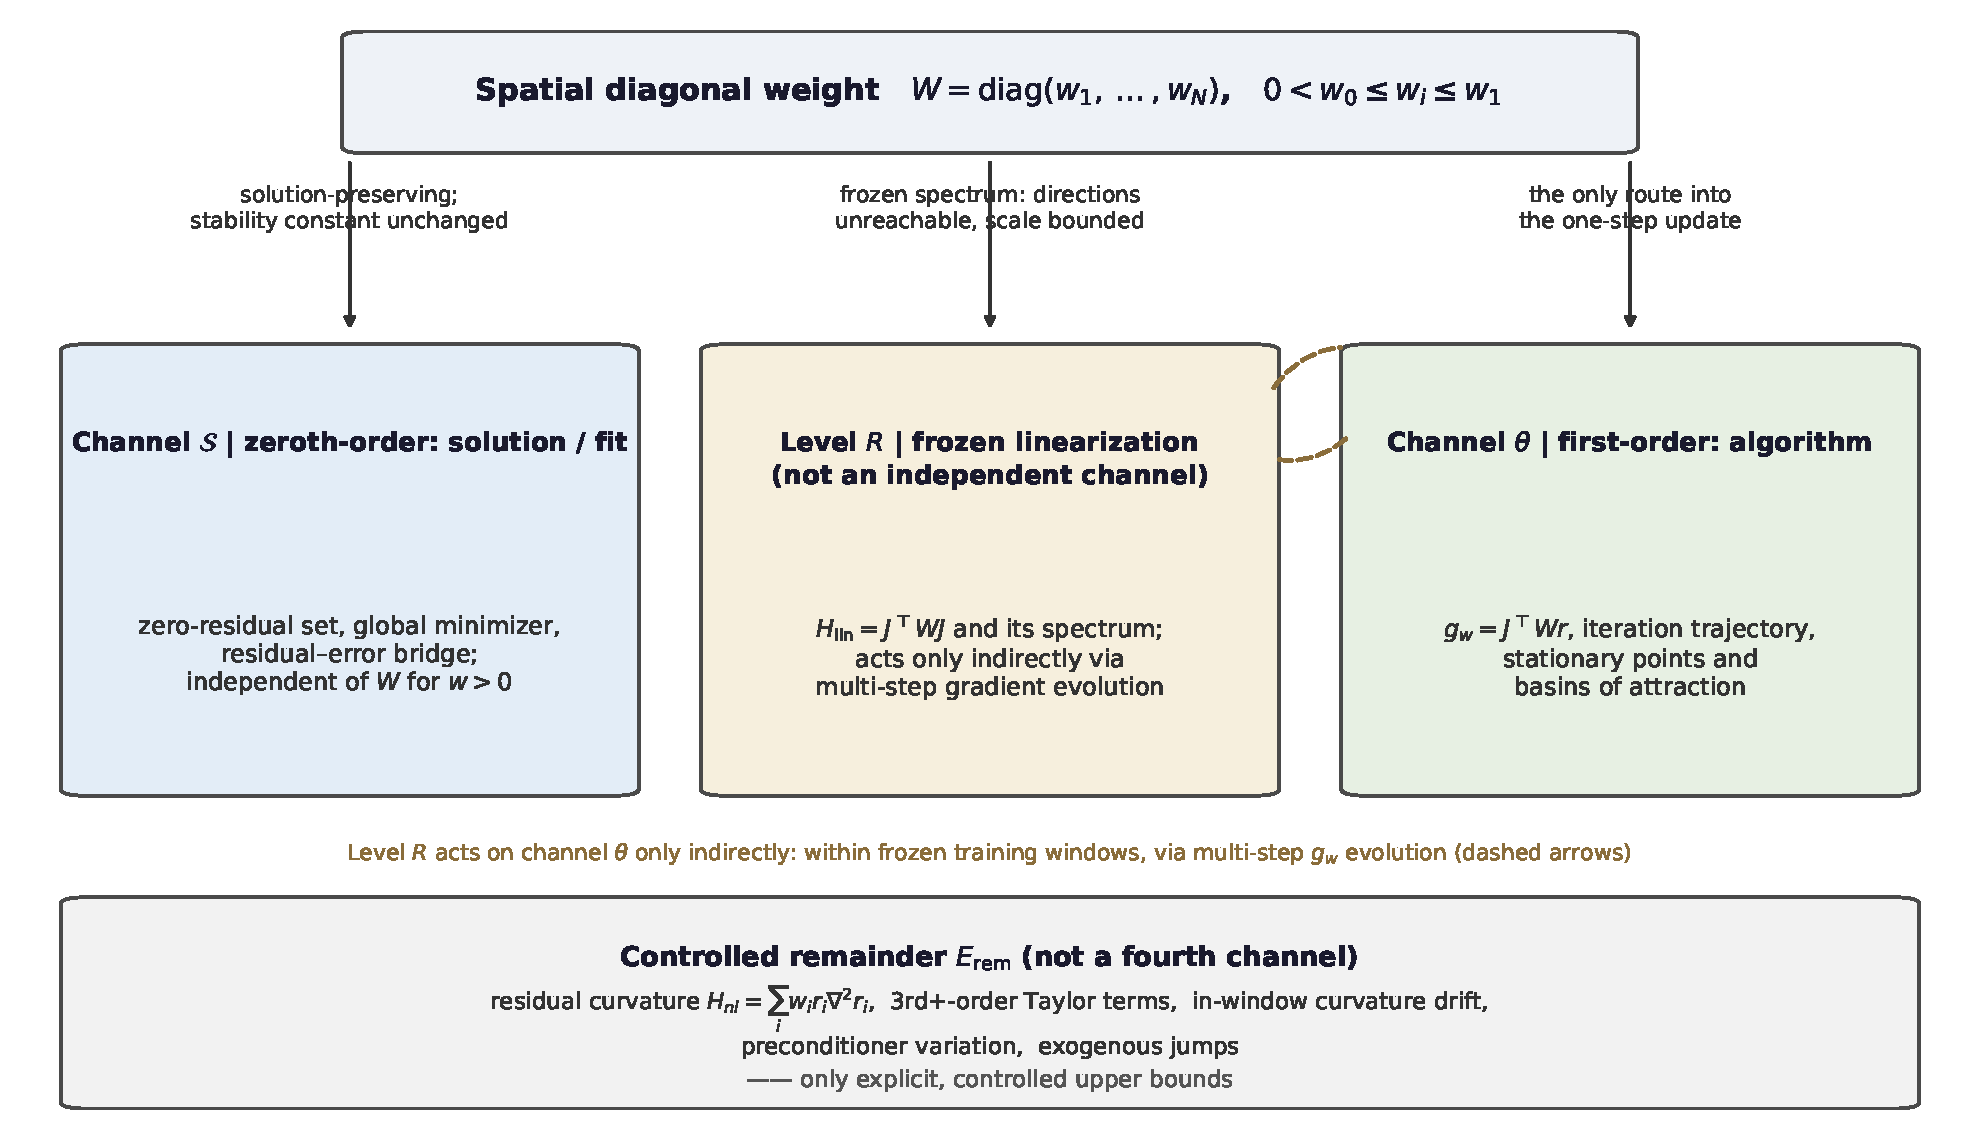
\includegraphics[width=0.99\linewidth]{fig_framework_en}
\caption{The separation of analysis levels used in this paper: the effects of spatial weights on the zeroth-order solution, the frozen linearization matrix, and the first-order gradient field belong to three different levels, and cross-level conclusions cannot serve as mutual evidence; the second-order level acts on the first-order level only indirectly, through multi-step evolution of the weighted gradient within a frozen training window (dashed line between boxes); higher-order and nonlinear terms are grouped into a bounded controlled remainder.}\label{fig:box}
\end{figure}

\subsection{Contributions}\label{sec:contrib}
For all standard results we cite and label them as ``restatement/application''; we claim contributions only for genuinely new parts. This paper adds the following three items:

\begin{enumerate}[label=(\arabic*),leftmargin=2em,itemsep=2pt]
\item \emph{Separation of analysis levels and admission principles}: by Taylor-expansion order, the effects of spatial weighting are separated into three levels---zeroth order (solution/well-posedness), first order (gradient/optimization dynamics), and second order (frozen linearization spectrum); this separation serves only to organize the analysis and prevent cross-level conclusions from being used as mutual evidence. Two principles, ``information closure'' and ``exogenous weights,'' delimit the admission boundary of the gradient-only algorithm class, explicitly placing out-of-class methods---natural gradient, K-FAC, trainable weights, adaptive sampling---outside the class and listing them one by one.
\item \emph{Spectral capability boundary at the second-order level}: we prove that spatially local diagonal weighting makes eigen-direction alignment of the frozen Gram matrix unreachable for an entire class (the correlation-matrix invariant $R(\tilde K_r)=R(K_r)$ is the core observation); on equicorrelation matrices the condition number is already optimal (Theorem~\ref{thm:equicorr}); and the effect is merely bounded rescaling along the original eigen-directions (the van der Sluis band). The only whitening weight, the non-local $\W\propto K_r^{-1}$, is dense and costs $O(N^3)$, making online training infeasible. Experiment 4.2 verifies this strictly and statically on a real frozen Burgers Jacobian: the improvement ratio of unconstrained positive diagonal weights relative to Jacobi equilibration is $r=\kappa^*_{\rm diag}/\kappa(R)\in[.76,.87]$ ($N\le512$, a multi-start lower bound; the true optimum is no smaller). Note that Jacobi equilibration $w_i\propto(K_r)_{ii}^{-1/2}$ is itself a spatially local diagonal weight, and the practitioner's starting point $w\equiv1$ has a condition number $\kappa(K_r)$ far above this (see the Experiment 4.2 triplet, Table~\ref{tab:f1d-triplet}). Experiment 4.3 serves as an in-training empirical corroboration. Under the default clipping configuration (clip=1), the down-weighting families worsen conditioning by $1.7$--$4.9\times$ ($3.0$--$4.9\times$ at the low viscosities $.001$/.005); with clipping off, the range is wider ($0.6$--$3.4$) and individual cells show improvement. Here $\kappa=\lambda_{\max}/|\lambda_{\min}|$ uses the algebraic-extremum convention with a Lanczos edge estimate, measuring the full Hessian rather than the frozen $H_{\rm lin}$; it is used only for cross-family ranking and does not constitute a strict dynamic verification of the theorem.
\item \emph{Controlled falsification experiments and characterization of capability boundaries}: we give a first-order directional criterion for up-weighting inside good basins and prove that the alignment angle cannot discriminate good from bad basins. Through $n=80$ paired McNemar tests (K=4 selection convention), we reject the hypothesis that ``down-weighting can raise the basin-entry probability'' (net rescue is negative for all three families; the uniform hit rate $.613$ is in fact higher than that of all weighted families; after Holm correction only down\_lin is significant, $p=.006$; the conclusion is robust under threshold perturbations $\tau\in[.05,.08]$, while $\tau<.05$ lacks power due to few good-basin samples). The uniform-scale component of down-weighting is absorbed by Adam's per-coordinate normalization, so its action is mainly gradient-scale modulation (suppressing gradient peaks and the hard-clipping rate); Experiment 5.8 detects a marginal signal of the residual spatial-redistribution effect (down\_lin raises the effective lr ceiling by a factor of two, exact two-sided $p=.0625$, asymptotic $\approx.043$, a consistent direction that does not reach $.05$ significance), so we do not claim that down-weighting is purely a scale modulator; down-weighting neither relaxes the stable step size nor improves basin entry, and terminal-state benefits appear only under spectral mismatch (see Section~\ref{sec:crosseqn}). Full $n=11$ experiments show that the terminal gain of fixed up-weighting strength is not significant; the post-hoc optimal $\beta^*$ is a descriptive observation (per-seed spread $1$--$100$, non-monotone in $\nu$), not a fixed strategy deployable before training; at fixed high strength ($\beta=8$), the \emph{group-median} terminal $L_2$ can even be worse than $\beta=1$ under configurations such as narrow width (e.g., the width-64 baseline, group median $.0043\to.018$), showing that the gain is sensitive to network width and fixed strength is not a universal benefit. A 1584-run degeneracy scan (Experiment 5.6) verifies gains at the stiff end and degradation to the error floor at the smooth end. When no ground truth is available at deployment, fixed single-projection scalars of the residual/loss self-evaluation type are limited by a Bayes error lower bound; a four-point XOR counterexample shows exact linear separation is impossible (minimum error $1/4$); the quantity $g_{et}$, which carries spatial-contrast structure, provides feasibility evidence for basin discrimination (proxy AUC $.971$, oracle AUC $.64$); it is a noisy discriminator whose value lies in filtering out obviously bad basins and reducing wasted refinement.
\end{enumerate}

\subsection{Organization and Statement Conventions}\label{sec:convention}
Section~\ref{sec:related} reviews the method genealogy and marks the boundaries; Section~\ref{sec:framework} gives notation, definitions, admission principles, and the zeroth-order baseline; Sections~\ref{sec:R}--\ref{sec:crosseqn} present, in order, the second-order spectral capability boundary, the first-order dynamics boundary, ground-truth-free basin discrimination, and cross-equation verification; Section~\ref{sec:conclusion} delineates the scope of applicability and concludes. Complete proofs are collected in Appendix~\ref{app:proof}, reproduction details in Appendix~\ref{app:repro}, full numerical tables in Appendices~\ref{app:data}--\ref{app:tables}, and the method-genealogy table and experiment atlas in Appendices~\ref{app:lineage}--\ref{app:atlas}.

The paper uses three statement-level labels: \textbf{[certain]} denotes structurally/algebraically always-true statements or direct applications of standard theorems; \textbf{[with probability $1-\delta$]} denotes statements that hold under explicit probabilistic assumptions, with $\delta$ controllable by the sample size; \textbf{[empirical $n=$]} denotes controlled-experiment conclusions, which always report the sample size $n$, dispersion (median and interquartile range, or Wilson confidence intervals), and the parameter grid actually tested. Strong assertion words (necessarily, impossible, unique, if and only if, guaranteed) are allowed only in the first two levels, and the required assumptions and the conclusion must appear together in the same paragraph; metaphorical wording does not enter conclusion sentences.

\FloatBarrier

\section{Related Work}\label{sec:related}
This section reviews the literature along four levels---solution, gradient, spectrum, basin---with an additional subsection on zeroth-order representation-level interventions; each subsection ends with a \emph{boundary} marking its relation to this paper. The complete genealogy table is in Appendix~\ref{app:lineage}.

\subsection{Rigorous Numerical Analysis and Error Bounds for PINNs}\label{sec:rel-error}
Rigorous analysis of PINN generalization error has become systematic: Mishra and Molinaro \cite{MishraMolinaro2020} combine forward stability with training error and collocation-sample counts to give generalization-error upper bounds; De~Ryck and Mishra give error estimates for Kolmogorov-type PDEs and a systematic survey of the numerical analysis of PINNs \cite{DeRyckMishra2022,DeRyckMishra2024}; Shin et al.\ prove convergence of PINN solutions for linear second-order elliptic and parabolic PDEs in the collocation-refinement limit \cite{Shin2020}. This line of work answers ``how training residuals and sample counts control the true error,'' corresponding to the residual--error bridge at the zeroth-order level of this paper. \emph{Boundary}: our residual--error bridge is a \emph{restatement of these standard stability estimates in spatially weighted norms}; we claim no originality. The only addition is making explicit that the stability constant is independent of the spatial weights, and thereby strictly separating ``the error of the solution'' from ``the improvement of the optimization trajectory.''

\subsection{Gradient Pathologies, Neural Tangent Kernels, and Convergence-Rate Mismatch}\label{sec:rel-ntk}
Wang, Teng, and Perdikaris \cite{WangTeng2020} systematically characterize the gradient-magnitude pathology of PINNs and mitigate it with learning-rate annealing; Wang, Yu, and Perdikaris \cite{Wang2020NTK} prove in the NTK framework that in the infinite-width limit training is governed by a deterministic kernel, that the convergence rates of \emph{different loss terms} are mismatched because the kernel eigenvalues differ, and accordingly propose eigenvalue-based calibration; the limitations of this linearized (lazy-training) view in nonlinear regimes are discussed in \cite{Bonfanti2024}. \emph{Boundary}: the above NTK mismatch occurs \emph{between different loss components}, whereas our eigen-direction boundary (Theorem~\ref{thm:local-cap}) concerns the effect of a spatial diagonal weight $\W$ on the frozen Gram eigen-directions \emph{within a single PDE residual}; the two are at different levels and their conclusions are complementary, not overlapping.

\subsection{Adaptive Collocation and Hard-Region Up-/Down-Weighting Routes}\label{sec:rel-weight}
On the \emph{up-weighting and adaptive sampling} side, RAR/RAD-type methods adaptively add collocation points according to residuals (a systematic comparison in \cite{Wu2022}, importance sampling in \cite{Nabian2021}, deep generative adaptive sampling in \cite{TangDAS2023}), and causal training \cite{Wang2022causal} weights by temporal causal structure; Self-Adaptive PINNs \cite{McClenny2020} adjust pointwise weights with trainable soft attention---because the weights are trainable, violating the exogenous-weight principle, they fall outside the admission class of this paper (Section~\ref{sec:framework}). On the \emph{down-weighting} side, Maddu et al.\ \cite{Maddu2021} characterize the multi-scale mismatch failure mode and mitigate it with inverse-Dirichlet weights; Liu et al.\ \cite{Liu2022down} \emph{de-emphasize} the network at discontinuities and focus on smooth regions; Wang et al.\ \cite{LessEmphasis2022} propose a curriculum-style strategy that pays less attention to high-loss regions. On the \emph{gradient-conflict} side, ConFIG \cite{ConFIG2025} resolves gradient conflicts via orthogonal projection during optimization. Recently, Si and Yan \cite{SiYan2025} argue from a primal--dual optimization perspective that pointwise weights are ``atomized,'' ignoring spatial correlation, and that only spatially coherent convolutional (non-local) weights can stably improve conditioning---independently corroborating, from the method side, our Theorem~\ref{thm:local-cap} conclusion that ``local weights are insufficient; effective whitening must be non-local.'' \emph{Boundary}: this paper does not propose yet another weighting strategy, but gives a unified verdict on ``what any spatially local weighting can and cannot do at the three levels of solution, gradient, and spectrum,'' and uses paired experiments to delineate the true operating ranges of up- and down-weighting.

\subsection{Condition Numbers, Optimal Weights, and Operator Preconditioning}\label{sec:rel-precond}
Under the frozen, linearized view, the program ``the condition number determines the convergence rate of first-order methods, so design preconditioners accordingly'' has systematic work. For linear, well-posed PDEs, van~der~Meer, Oosterlee, and Borovykh \cite{vanDerMeer2020} prove convexity of the weighted objective functional and give the optimal scaling---the most direct precedent for ``weighting does not change well-posedness, only the conditioning scale.'' de~Ryck et al.\ \cite{deRyckOp2024} analyze the training of physics-informed machine learning from an operator-preconditioning viewpoint: in frozen linear models they relate the discrete Gram matrix to the Hermitian square of the differential operator, give an $O(\kappa\log\varepsilon^{-1})$ gradient-descent iteration complexity, and reduce the condition number to about $1$ by operator-spectrum scaling or dense inverse whitening; preconditioned PINNs (PCPINN \cite{PCPINN2024}) likewise diagnose training via the condition number, borrowing classical preconditioners of PDE discrete operators (e.g., incomplete LU) to improve the solve---the original work notes that ILU does not guarantee a strict decrease of the condition number, though it empirically promotes convergence. On the side of optimal diagonal scaling, the optimal positive diagonal preconditioner of a given matrix can be computed exactly via semidefinite programming and approximated in nearly linear time \cite{Qu2025ODP,Jambulapati2020,Gao2024SODP}; which matrix classes are already optimal under diagonal scaling also has classical characterizations \cite{ForsytheStraus1955,Shapiro1982,LivneGolub2004}. The Kronecker block-diagonal preconditioner for multiphysics PINNs \cite{KroneckerPINN2026} acts at the cross-equation block level rather than pointwise within a field. \emph{Boundary}: the above preconditioners are either dense, non-local, operator-level transformations depending on the linearization point, or they modify the optimizer or network architecture; ``non-local preconditioning can bring the condition number down to about $1$'' has already been answered by them, and we do not claim priority for the feasibility of spectral whitening. What is new here is its \emph{complement}: why the most engineering-common restricted class of \emph{spatially local, pointwise diagonal} weights cannot do it (the correlation-matrix invariant and the van~der~Sluis bound of Theorem~\ref{thm:local-cap}). In addition, our zeroth-order weighted-norm two-sided squeeze can be seen as an extension of the convexity conclusion of \cite{vanDerMeer2020} to the nonlinear local case; the second-order eigenvalue-scale bounds further show that even in the linear case, the net effect of spatially \emph{allometric} (non-multiplicative-constant) weighting on the condition number remains two-sidedly indefinite. The division of labor with the optimal-diagonal-preconditioning literature: the latter computes the optimal diagonal scaling for a \emph{given} matrix (a computational problem), whereas this paper characterizes what the \emph{entire class} of spatially local diagonal weights cannot reach in terms of eigen-directions (a capability boundary), and Experiment 4.2 measures the actual distance from the optimal scaling to whitening.

\subsection{Basin Reachability, Curriculum, and Homotopy}\label{sec:rel-curriculum}
Bengio et al.\ \cite{Bengio2009} establish the general view that curriculum learning is continuation and affects the quality of local minima; the optimization theory of continuation methods traces back to Gaussian homotopy and graduated optimization \cite{Mobahi2015,Hazan2016}, and gradient methods converge to minimizers almost surely under isolated-saddle conditions \cite{Lee2016}. Krishnapriyan et al.\ \cite{Krishnapriyan2021} systematically characterize PINN failure modes and significantly reduce error with curriculum/sequential regularization; a systematic analysis of PINN training difficulty from the loss-landscape perspective is in \cite{Rathore2024}; other work points out that a substantial part of the failure modes stems from single-precision floating-point error rather than the loss landscape itself, and is eliminated by switching to FP64 \cite{FP64Xu2025}---complementary to our perspective: precision determines whether the residual can be driven down, and basin structure determines whether what is driven down is the true solution. On the pseudo-solution side, Rohrhofer et al.\ \cite{Rohrhofer2022} point out that PINNs of dynamical systems minimize residuals near trivial fixed points, letting non-physical solutions dominate the basins of attraction; Wang et al.\ \cite{WangPseudo2026} address pseudo-solutions with ``small residual but physically wrong solution,'' revealing and circumventing them via pseudo-time stepping and resampling; R3 sampling, which mitigates propagation failure by resampling, also belongs to this line \cite{Daw2022Evo}. The phenomenon itself---that PINNs have pseudo-solution basins, and that continuation/resampling/domain shrinking helps avoid them---is attributed to the above literature. Closest to Section~\ref{sec:methods} of this paper is Musah \cite{Musah2026}: in multi-field constrained systems it independently and systematically reports that a single aggregated residual selects worse solutions at high frequency, and proposes lexicographic admissibility gating. \emph{Boundary}: we concede the general observation that ``a single scalar residual cannot reliably select solutions''; what is new is a rigorous four-point counterexample in the context of spatial-weighting basin discrimination, together with structural quantities that do not rely on residual self-evaluation.

\subsection{Zeroth-Order Representation-Level Interventions: Hard-Constraint Ansatz, Coordinate Transforms, and Initialization}\label{sec:rel-repr}
Another line of work does not modify loss weights but directly modifies the zeroth-order representation of the network. First, \emph{hard-constraint trial functions/output transforms}: distance functions and R-functions construct annihilating factors that exactly satisfy Dirichlet/Neumann/Robin conditions pointwise at the output \cite{Sukumar2022distance}, or encode linear PDEs as output-layer hyperplanes so that the equation is satisfied pointwise \cite{Leng2022hyperplane}; second, \emph{input/coordinate transforms}: variable scaling or coordinate mappings (translations and scalings) alleviate thin layers and stiffness---Guan and Elman \cite{GuanElman2024} analytically explain via NTK how input transforms change the effective kernel; third, \emph{initialization and representation bandwidth}: random initialization and deep ensembles are used to discover multiple solutions of PDEs \cite{Zou2025ensemble}. \emph{Boundary}: the above constructions respectively change the boundary lifting, annihilating factor, or coordinate mapping of the forward ansatz, or the initial values/frequencies---that is, they all act at the zeroth-order representation level; they are isolated single-level interventions that neither give an irreplaceable cross-level classification of ``zeroth-order representation---second-order spectrum---first-order optimization,'' nor distinguish ``expressible'' from ``reachable.''

\FloatBarrier

\section{Notation, Definitions, and the Zeroth-Order Baseline}\label{sec:framework}

\subsection{Notation and the Weighted Training Objective}\label{sec:notation}
Let the network $u(x;\theta)$ ($\theta\in\R^p$) approximate the solution $u^*$ of the PDE $\mathcal N[u]=0$; in all experiments of this paper the initial/boundary conditions are exactly satisfied by a hard-constraint ansatz (a zeroth-order representation-level intervention; see Section~\ref{sec:rel-repr}), so the residual vector contains only interior collocation points. At collocation points $\{x_i\}_{i=1}^{N}$ define $r(\theta)=(r_1,\dots,r_N)^\top$, $r_i=\mathcal N[u](x_i;\theta)$, and the Jacobian $J(\theta)=\partial_\theta r\in\R^{N\times p}$. A \emph{spatial diagonal weight} is $\W=\diag(w_1,\dots,w_N)$, $w_i\ge0$ given by an exogenous rule: the pointwise argument is the residual contrast $t_i$ (Eq.~\eqref{eq:t-contrast}), and the global strength $\beta$ is an exogenous hyperparameter; weights are frozen between snapshots and not jointly trained with $\theta$ (corresponding to the frozen branch of Principle~II of Definition~\ref{def:admit}; the online-recomputation convention of the basin-entry experiments is an exploratory design---see the protocol statement in Section~\ref{sec:theta-exp} and the freezing implementation details in Appendix~\ref{app:repro}). The weighted training objective uses the empirical mean (consistent with the standard convention of the original PINN MSE and optimal weighted losses \cite{Raissi2019,vanDerMeer2020}):
\begin{equation}\label{eq:lw}
L_{\W}(\theta)=\tfrac{1}{2N}\sum_{i=1}^{N}w_i r_i^2=\tfrac{1}{2N} r(\theta)^\top \W r(\theta).
\end{equation}
Throughout, $\W$ belongs to the positive-definite diagonal cone $\mathcal W_+=\{\W:0<w_0\le w_i\le w_1<\infty\}$, with weight condition number $\kappa_{\W}=w_1/w_0$; all weight families deployed in this paper strictly satisfy $w_i>0$ (see Section~\ref{sec:family}). Under the empirical-mean convention the first-order gradient and Hessian are
\begin{equation}\label{eq:h-split}
g_{\W}:=\tfrac1N J^\top\W r,\qquad
H_{\W}:=\nabla_\theta g_{\W}
=\underbrace{\tfrac1N J^\top\W J}_{H_{\rm lin}}
+\underbrace{\tfrac1N\sum_{i=1}^{N}w_i r_i\,\nabla_\theta^2 r_i}_{H_{\rm nl}} ,
\end{equation}
where $H_{\rm lin}=\tfrac1N J^\top\W J$ is the Gauss--Newton term (containing only first derivatives of the residual, independent of the residual magnitude) and $H_{\rm nl}$ is the residual-curvature term (linear in the residual, vanishing as the residual tends to zero); this is the standard Gauss--Newton decomposition. \emph{Common-factor convention}: $1/N$ is a direction-independent common positive scalar that changes neither eigenvectors, inertia indices, condition numbers, nor null spaces; hence from the matrix-spectrum characterization onward, wherever only directions, spectral structure, and inertia are involved, we absorb this common factor into the notation and still write $J^\top\W J$. Note that $J$, $J^\top J$, and the Fisher information matrix $F(\theta)=J^\top J$ (equal-weight case) all \emph{exclude} the spatial weight $\W$.

\noindent\emph{Norm conventions for the whole paper.} Euclidean vector norm $\norm v=(v^\top v)^{1/2}$; weighted norm under a preconditioner $P_t\succ0$, $\norm v_{P_t}^2=v^\top P_t v$ (gradient descent with $P_t=I$ reduces to the Euclidean norm); function-space $\norm f_{L^2}=(\int|f|^2)^{1/2}$, weighted $\norm f_{L^2(w)}=(\int w|f|^2)^{1/2}$, whose discrete counterparts are the $\ell^2$ norm and $\norm r_\infty=\max_i|r_i|$; matrices default to the spectral norm $\norm A_2$, with the Frobenius norm $\norm A_F$ explicitly marked where used. \emph{Whitening convention (throughout the optimization-dynamics analysis)}: for a positive-definite preconditioner $P_t\succ0$, write the whitened quantities $\wt g:=P_t^{1/2}g$, $\wt H_{\rm lin}:=P_t^{1/2}H_{\rm lin}P_t^{1/2}$, $\wt H_{\rm nl}:=P_t^{1/2}H_{\rm nl}P_t^{1/2}$; after whitening all norms are Euclidean, and condition-number factors appear only once when conclusions are transferred back to the original space (for $P_t=I$ everything degenerates to the identity).

\subsection{Weight Families and the Rational Up-Weighting Family}\label{sec:family}
We use the pointwise \emph{residual contrast}
\begin{equation}\label{eq:t-contrast}
t_i=\frac{|r_i|}{\operatorname{median}|r|+\epsilon}\ge0,\qquad \epsilon>0
\end{equation}
as the argument; $\operatorname{median}|r|$ is the median of the residual magnitudes over all $N$ collocation points, and $\epsilon=10^{-12}$ only guards against division by zero and plays no role in magnitudes (implementation convention in Appendix~\ref{app:repro}). This paper compares six weight families: three up-weighting families (rational, linear, band), two down-weighting families (down\_lin, down\_inv), and the uniform family. The main family is the \emph{rational up-weighting family}. Write $q=t/(1+t)\in[0,1)$, $\bar q(t)=\min\{t,1\}$ (truncated to $[0,1]$), and $\mathbf 1\{\cdot\}$ for the indicator function; the code implementation and all experiments uniformly adopt the following explicit forms:
\begin{equation}\label{eq:families}
\begin{aligned}
&\text{rational:}\ \ w=1+(\beta-1)q=\tfrac{1+\beta t}{1+t},
&\text{linear:}\ \ w&=1+(\beta-1)\bar q(t),\\
&\text{band:}\ \ w=1+(\beta-1)\mathbf 1\{q>\tfrac12\},
&\text{uniform:}\ \ w&\equiv1,\\
&\text{down\_lin:}\ \ w=1-(1-\beta^{-1})q,
&\text{down\_inv:}\ \ w&=\tfrac{1}{1+(\beta-1)q}=\tfrac{1+t}{1+\beta t}.
\end{aligned}
\end{equation}
The three up-weighting families are all bracketed in $[1,\beta]$, and the two down-weighting families in $[\beta^{-1},1]$ (endpoints are $t\to\infty$ limits, or are attained via truncation/indicator); the theoretical analysis takes rational as the main family, with the other five as controlled comparisons, and the algebraic forms in both paper and code always follow Eq.~\eqref{eq:families}.

\begin{definition}[Rational up-weighting family and $\phi$]\label{def:w}
For contrast $t\ge0$ and strength $\beta\ge1$, the rational up-weighting function and the \emph{gradient-component contrast} are
\begin{equation}\label{eq:rational}
w(t;\beta)=\frac{1+\beta t}{1+t},\qquad \phi(t;\beta)=t\,w(t;\beta)=\frac{1+\beta t}{1+t}\,t .
\end{equation}
Here $\phi=tw$ is the contrast magnitude of the weighted gradient component $w_i r_i J_i$ (a first-order-level object); in Mechanism~A the redistribution of gradient energy by up-weighting is realized through $\partial_\beta w$, unrelated to $\phi'$ (see Section~\ref{sec:theta-mechA}). $\phi=tw$ must be distinguished from the \emph{loss-level magnitude} $t\sqrt w$ (the contrast of the single-point loss density $\sqrt w\,|r|$, a zeroth-order-level object with the same convention as the two-sided residual--error bridge bound); the two differ by a factor $\sqrt w$ and must not be mixed.
\end{definition}

Rational up-weighting satisfies $w(0)=1$, $w(\infty)=\beta$, $w'(t)=(\beta-1)/(1+t)^2\ge0$, so $1\le w\le\beta$, monotone and boundedly saturating in $t$. Linear down-weighting is $w^{dn}_{lin}=1-(1-1/\beta)q\in[1/\beta,1]$ (consistent with the code implementation in Eq.~\eqref{eq:families}), and inverse down-weighting is $w^{dn}_{inv}(t)=(1+t)/(1+\beta t)\in[1/\beta,1]$, the dual of the up-weighting rational form in the numerator/denominator-swap sense; the two share endpoints $\{1,1/\beta\}$ and both decrease in $t$ (opposite to the up-weighting families). The uniform family is identically $1$.

The single-point weighted loss density of the main family is $\Psi_2(t)=w(t)\,t^2$ (weighted $L^2$ in $t$, with equivalent weight exactly $w$), and this convention is used throughout. Along a single residual radial direction, $\Psi_2''(t)=2(1+3\beta t+3\beta t^2+\beta t^3)/(1+t)^3>0$, so $\Psi_2$ is strictly \emph{radially convex along the one-dimensional residual-magnitude direction} over the entire region $\beta\ge1,t\ge0$. This convexity is only a design self-check property of the one-dimensional residual-magnitude radial; it does not imply any (local or global) convexity of the optimization landscape in parameter space $\theta$.

\subsection{Admission to the Gradient-Only Algorithm Class: Information Set and Two Principles}\label{sec:admit}
The theoretical analysis of this paper is restricted to the \emph{gradient-only class}: algorithms whose single-step parameter update reads only the weighted gradient $g_\W$ at the current point (and auxiliary states constructed from gradients), and does not directly read the Hessian, the Jacobian spectrum, or the scalar loss landscape. Typical representatives include gradient descent (GD), GD with momentum, Adam and its variants; quasi-Newton methods such as L-BFGS can be admitted if their step-size rules are based on $|g_\W|$, but fall outside the class if the line search directly reads $L_\W$ (see the out-of-class method list in Definition~\ref{def:admit}).

\begin{definition}[Information set and two principles]\label{def:admit}
Let the single-step update be $\theta_{k+1}=\theta_k-\eta_k A_k g_\W(\theta_k)$, where $A_k$ is a preconditioning matrix. The algorithm belongs to the gradient-only class if and only if the following two principles hold:
\begin{enumerate}[label=\textup{(P\arabic*)},leftmargin=2em]
\item \emph{Information closure}: $A_k$ and the step size $\eta_k$ depend only on the past gradient sequence $\{g_\W(\theta_j)\}_{j\le k}$ (and auxiliary states constructed from gradients, such as momentum and Adam's second moment), and do not directly read the scalar loss value $L_\W$, $J(\theta_k)$, $H_{\rm lin}(\theta_k)$, or their spectra.
\item \emph{Exogenous weights}: the spatial weight $\W$ is frozen within a training window or given by an exogenous slowly-varying process, and does not depend on the current parameter $\theta_k$ through a differentiable function; i.e., $\nabla_{\theta_k}\W=0$ (frozen) or $\|\nabla_{\theta_k}\W\|$ is explicitly controlled by a small quantity (slowly varying; quantitative convention in Assumption~\ref{ass:ctrl}(Q4) and Remark~\ref{rem:adam-drift}).
\end{enumerate}
\end{definition}

The point of the two principles is: under the tightened (P1)(P2), the only differential route by which $\W$ enters a single-step update is the weighted gradient $g_\W=J^\top\W r$; the matrix $H_{\rm lin}=J^\top\W J$ is not directly read by a single step. This is the algorithmic premise of the level separation throughout the paper. If an algorithm directly reads $L_\W$ (e.g., standard Armijo line search), then $L_\W$ itself carries $\W$, the ``only route'' no longer holds, and such algorithms fall outside the class.

\emph{Out-of-class methods} (violating (P1) or (P2)) include: natural gradient ($A=G^{-1}$ directly reads the Fisher information matrix, violating P1), K-FAC (block-approximate Fisher, violating P1), \emph{scalar-loss-based line search/step-size schedules} (e.g., standard Armijo backtracking, violating P1), trainable weights ($\W=\W(\theta)$ differentiable, violating P2, e.g., Self-Adaptive PINNs \cite{McClenny2020}), adaptive sampling RAR/RAD (changing the collocation set rather than fixed weights---another kind of intervention), and dense operator preconditioning (directly reading the differential operator's spectrum, violating P1). These methods are not covered by the theory of this paper, but their levels of action can be located by the above stratification: natural gradient/preconditioning acts at the second-order level (trying to whiten $H_{\rm lin}$), trainable weights act at the interface of the first- and second-order levels ($\W$ varying with $\theta$ introduces extra gradient terms), and adaptive sampling changes the collocation measure (a zeroth-order object change).

\subsection{Zeroth-Order Level: Solution-Set Invariance and the Residual--Error Bridge}\label{sec:Schan}
After fixing the weight families (Section~\ref{sec:family}) and the algorithmic admission class (Section~\ref{sec:admit}), this section fixes the zeroth-order objects that depend on neither: the zero-residual solution set, the global minimum, and the residual-to-error stability bridge. They are the common baseline of the level framework---the second-order (Section~\ref{sec:R}) and first-order (Section~\ref{sec:theta}) analyses both superimpose weighting and algorithmic effects on this baseline; since the zeroth-order objects do not change with $\W$ and the conclusions are short, they do not occupy a chapter of their own. The following results are restatements of standard stability estimates in spatially weighted norms; we claim no originality.

\begin{proposition}[Zero-solution-set invariance]\label{prop:zero}
Let $\W=\diag(w_i)$ satisfy $w_i>0$ for all $i$. Then the zero-residual solution sets of the weighted loss $L_\W(\theta)=\tfrac12 r(\theta)^\top\W r(\theta)$ and the equal-weight loss $L_I(\theta)=\tfrac12\|r(\theta)\|^2$ are exactly the same; when zero residual is attainable (well-posed with sufficient representation), the global-minimizer sets of both equal $\{\theta:r(\theta)=0\}$.
\end{proposition}
The proof is a componentwise algebraic verification; see Appendix~\ref{app:proof}.

The meaning of Proposition~\ref{prop:zero} is: spatial weighting changes neither ``which parameter points are exact solutions of the equation'' nor the location of the global minimum (in well-posed problems where zero residual is attainable). Therefore, claiming that ``weighting improves optimization'' cannot rest on ``zero-solution-set invariance''---zeroth-order objects and first-order dynamics are two independent levels.

\begin{assumption}[Well-posedness input, citational]\label{ass:wellposed}
Suppose the linearization of the PDE operator $\mathcal N$ near the solution $u^*$ is boundedly invertible, and there exists a stability constant $C_{\rm stab}>0$ such that for sufficiently small residual $r=\mathcal N[u_\theta]$,
\begin{equation}\label{eq:bridge}
\|u_\theta-u^*\|_{L^2}\le C_{\rm stab}\,\|r\|_{L^2},
\end{equation}
where $\|r\|_{L^2}^2=\int_\Omega |\mathcal N[u_\theta](x)|^2 dx$. Such estimates are a \emph{standard input} of PINN error analysis, not a result of this paper: for the general case see \cite{MishraMolinaro2020,DeRyckMishra2022}; rigorous proofs for linear second-order elliptic/parabolic equations are in \cite{Shin2020}; explicit DNN error estimates for the viscous Burgers equation (the main testbed of this paper) are in \cite{Akram2025}. For clean norm estimates of the Burgers traveling-wave internal layer we do not assert a proof, and only take formal magnitudes (convention in Appendix~\ref{app:proof}).
\end{assumption}

\begin{proposition}[Weighted version of the residual--error bridge]\label{prop:bridge}
Under Assumption~\ref{ass:wellposed}, for the weighted norm $\|r\|_{L^2(w)}^2=\int_\Omega w(x)|\mathcal N[u_\theta](x)|^2 dx$, when $w_0\le w(x)\le w_1$ the two-sided squeeze
\begin{equation}\label{eq:bridge-weighted}
w_0^{1/2}\|r\|_{L^2}\le \|r\|_{L^2(w)}\le w_1^{1/2}\|r\|_{L^2}
\end{equation}
holds. Hence the stability constant $C_{\rm stab}$ is independent of the spatial weights: weighting only rescales the residual norm (introducing at worst a $w_0^{-1/2}$ scale factor) and does not change well-posedness.
\end{proposition}
The proof is a componentwise algebraic verification; see Appendix~\ref{app:proof}.

The meaning of Proposition~\ref{prop:bridge} is: spatial weighting does not change the well-posedness of the PDE, only the scale of the residual norm. Down-weighting ($w_0<1$) amplifies the stability constant in the weighted norm (at worst by $\sqrt{\beta}$), but this is a scale effect, not a change of well-posedness. Up-weighting ($w_1>1$) does not loosen the original $L^2$ stability constant. This distinction is the baseline for the later ``cost of down-weighting'' analysis. (Notation: $C_{pde}$, $C_{loc}$ in the appendix proofs have the same convention as $C_{\rm stab}$ here---all are norm bounds of the (linearized) operator inverse; quadrature/sampling error between discrete collocation and continuous integration is counted in the $\varepsilon_{quad}$ of Lemma~\ref{lem:3comp}.)

\begin{corollary}[Norm bounds and the down-weighting bound]\label{cor:normbd}
Under the up-weighting normalization ($w_0=1$, $w_1=\beta$), $\|r\|_{L^2}\le\|r\|_{L^2(w)}\le\sqrt\beta\,\|r\|_{L^2}$ and the original $L^2$ stability constant is unchanged; under down-weighting ($w_0=1/\beta$, $w_1=1$), $\beta^{-1/2}\|r\|_{L^2}\le\|r\|_{L^2(w)}\le\|r\|_{L^2}$ and $\|u_\theta-u^*\|_{L^2}\le C_{\rm stab}\sqrt\beta\,\|r\|_{L^2(w)}$: down-weighting amplifies the stability constant in the weighted norm by at most $\sqrt\beta$.
\end{corollary}
The proof is a direct substitution; see Appendix~\ref{app:proof}.

\begin{corollary}[Nonlinear-remainder bound]\label{cor:nonlin}
Suppose $-r_\theta=\Lop_*e+R_2$ (where $\Lop_*$ is the linearized operator of Assumption~\ref{ass:wellposed} and $e=u_\theta-u^*$) with $\|R_2\|\le L_N\|e\|_{L^2}^2$. Then for an error radius $\rho_{\rm bas}$ satisfying $2C_{\rm stab}L_N\rho_{\rm bas}\le\tfrac12$, within $\|e\|_{L^2}\le\rho_{\rm bas}$ one has $\|e\|_{L^2}\le 2C_{\rm stab}w_0^{-1/2}\|r_\theta\|_{L^2(w)}$. For the Burgers traveling wave $L_N=1/(2\nu)$; the formal scaling $\rho_{\rm bas}(\nu)=O(\nu^2)$ and its limitations are given in Appendix~\ref{app:proof}.
\end{corollary}
The proof and explicit estimates of $C_{loc},\rho_{\rm bas}(\nu),R_r(\nu)$ are in Appendix~\ref{app:proof}.

\begin{lemma}[Three-component decomposition]\label{lem:3comp}
Writing $u_m^*$ for the best representation in the network class and $u_{\mathcal S}$ for the intermediate quantity accounting for sampling and quadrature, the total error decomposes as $\|u^*-u_{\theta_T}\|\le\varepsilon_{app}+\varepsilon_{gen}+\varepsilon_{quad}+\varepsilon_{opt}$: the representation error $\varepsilon_{app}$ is determined solely by representation capacity and is independent of $w$; the generalization/quadrature terms $\varepsilon_{gen}+\varepsilon_{quad}$ acquire only an $O(\sqrt\beta)$ constant dependence via Proposition~\ref{prop:bridge}; only the optimization term $\varepsilon_{opt}$ is strongly coupled to the weighting dynamics.
\end{lemma}
The proof is in Appendix~\ref{app:proof}.

\FloatBarrier

\section{Second-Order Level: Spectral Capability Bounds of Local Diagonal Weights}\label{sec:R}

This section studies how the spectrum of the frozen linearization matrix $H_{\rm lin}=J^\top\W J$ varies with the spatial diagonal weight $\W$. The core question is: \emph{can one make this quadratic form less ill-conditioned merely by assigning different weights to different spatial collocation points?} The answer is: local diagonal weights can change the eigenvalue scales but cannot change the correlation structure among collocation points (the eigen-directions), which is precisely the root of ill-conditioning in stiff problems. We first give the frozen-linearization framework, then prove the core theorem, and finally verify twice: by a static $N$-scan on a real Burgers Jacobian and by a dynamic record of the in-training Hessian condition number.

\subsection{Global Assumptions and the Frozen-Linearization Framework}\label{sec:R-frame}

The following three groups of assumptions run through the theoretical analysis at the second- and first-order levels, with their nature explicitly labeled.

\begin{assumption}[G-A representability, static]\label{ass:GA}
Given a Fourier bandwidth $\sigma$ covering the shock scale $O(\nu)$, there \emph{exists} in the network class a parameter $\theta_m^*$ with $\|u^*-u(\cdot;\theta_m^*)\|\le\varepsilon_{app}$ (the representation component of the three-component decomposition, Lemma~\ref{lem:3comp}). This \emph{existence} is a standard consequence of universal approximation of neural networks and PINN consistency/generalization-error estimates \cite{Shin2020,MishraMolinaro2020,DeRyckMishra2024}, and \emph{does not depend on the specific equation}; this paper asserts only existence, not that training can find it (reachability belongs to G-B). \emph{Only the scaling constants depend on the equation}: for the reference solution $u^*=-\tanh(x/(2\nu))$, its $k$-th derivative carries the factor $\nu^{-k}$, so the width and bandwidth needed for a fixed $\varepsilon_{app}$ grow as $\nu\downarrow$; this is the intrinsic difficulty of the equation, unrelated to weights.
\end{assumption}

\begin{assumption}[G-B basin reachability, Phase~0, probabilistic]\label{ass:GB}
Let $p_{entry}=\Pr_{\theta_0,\mathcal S}[\theta(T_0)\in B(u^*);\mathcal C_\sigma,\mathcal O]$ denote the probability of entering the true-solution basin by time $T_0$ under representation curriculum $\mathcal C_\sigma$ and optimizer $\mathcal O$. We do not assume $p_{entry}=1$; we only study its dependence on $\sigma$, width, initialization, and the number of multi-starts $K$.
\end{assumption}

\begin{assumption}[G-C in-basin local benignity, Phase~1, weakened version]\label{ass:GC}
Upon entering $B(u^*)$, with weights frozen or \emph{exogenously slowly varying} (our conclusions target frozen $\W$, or exogenous slowly-varying $\W$ triggered by training schedules/unweighted quantities; online-adaptive or trainable $\W(\theta)$ violates Principle~II, lies outside the gradient-only class, and is left to future work):
\par(i)~\emph{Effective-subspace nondegeneracy}: on the gradient Krylov subspace $V_g=\spanop\{g,H_{\W}g,\ldots\}$, the smallest Ritz value satisfies $\lambda_{\min}(V_g^\top H_{\W}V_g)\ge\lambda_*(\nu)>0$ (positive-definiteness of the full-space Hessian is not required);
\par(ii)~\emph{Bounded drift within the training window}: there exists $\varepsilon_{NTK}<1$ such that $\sup_{0\le t\le T_1}\|K_r(t)-K_r(0)\|/\|K_r(0)\|\le\varepsilon_{NTK}$ (finite-width training window; the $m\to\infty$ asymptotic is not required);
\par(iii)~\emph{{\L}ojasiewicz local benignity}: within an error radius $\rho_{\rm bas}(\nu)$ (existence and formal scaling in Corollary~\ref{cor:nonlin}), $\|\nabla L_{\W}\|\ge c_L|L_{\W}-L_{\W}^\star|^\vartheta$, $\vartheta\in[1/2,1)$. For Fourier-feature networks with real-analytic activations (e.g., sin, tanh), the residual is a real-analytic function of the parameters, and analyticity \emph{implies} a local {\L}ojasiewicz inequality, so (iii) is closer to a corollary than an extra assumption.
\emph{G-C never requires, nor implies, that spatial weighting can achieve spectral whitening} (spectral whitening means weighting that brings the condition number of the frozen Gram to $1$, i.e., $\W\propto K_r^{-1}$; it is unreachable for the entire class of spatially local weights, see Theorem~\ref{thm:local-cap}).
\end{assumption}

Suppose the network residual is sufficiently smooth within the training window ($r\in C^{2,1}$, i.e., second derivatives Lipschitz, which holds for smooth activations). The single-step update of a general first-order algorithm is
\begin{equation}\label{eq:onestep}
\theta_{k+1}=\theta_k-\eta P_t g_k,\qquad P_t\succ0,
\end{equation}
where $P_t$ is constructed from the information set at step $k$: gradient descent $P_t=I$; Adam $P_t=D_t^{-1}$ (with $D_t=\diag(\hat v_t)+\epsilon I$ the bias-corrected second-moment diagonal); fixed-step L-BFGS $P_t=B_k^{-1}$. Equation~\eqref{eq:onestep} idealizes momentum-based algorithms by ignoring the momentum direction (i.e., treating Adam as a diagonally preconditioned gradient step); this idealization does not change the level of the conclusions---under Adam the quantitative in-window bound of Lemma~\ref{lem:linrec} degenerates in any case to a non-expansive upper bound (Remark~\ref{rem:adam-drift}). Taking the unique symmetric positive-definite square root $P_t^{1/2}$, define the \emph{whitened quantities}
\begin{align}
\wt g:=P_t^{1/2}g,\quad \wt H_{\rm lin}:=P_t^{1/2}H_{\rm lin}P_t^{1/2},\quad
\wt H_{\rm nl}:=P_t^{1/2}H_{\rm nl}P_t^{1/2},\quad \wt H_{\W}:=\wt H_{\rm lin}+\wt H_{\rm nl}.\label{eq:white}
\end{align}
The whitened similar form of the homogeneous operator $M=I-\eta H_{\rm lin}P_t$ is $\wt M=I-\eta\wt H_{\rm lin}$; since $\wt H_{\rm lin}$ is symmetric positive semidefinite, $\wt M$ is a \emph{symmetric} matrix and the Euclidean spectral theorem applies directly. The Krylov subspace generated by the \emph{linearized} principal part is called the linearized walk subspace $\wt V_g^{lin}:=\mathcal K(\wt H_{\rm lin},\wt g_k)=\spanop\{\wt g_k,\wt H_{\rm lin}\wt g_k,\ldots\}$; taking its Euclidean orthonormal basis $Q$, define the whitened smallest/largest Ritz values $\lambda_V^{(P)}:=\lambda_{\min}(Q^\top\wt H_{\rm lin}Q)$, $\widehat\lambda_V^{(P)}:=\lambda_{\max}(Q^\top\wt H_{\rm lin}Q)$.

\begin{corollary}[Whitened nondegeneracy: weighting does not change the null space]\label{cor:ker}
For any $\W\succ0$ and positive-definite $P_t$: (i)~$\ker\wt H_{\rm lin}=P_t^{-1/2}\ker J$, where the right-hand side contains no $\W$---spatial weighting can neither create nor annihilate null-space directions; (ii)~Loewner monotonicity: $\W_1\preceq\W_2\Rightarrow Q^\top\wt H_{\rm lin}^{(1)}Q\preceq Q^\top\wt H_{\rm lin}^{(2)}Q$ (for any fixed Euclidean orthonormal basis $Q$); (iii)~nondegeneracy of the linearized walk subspace always holds: $\lambda_V^{(P)}>0$ is an algebraic corollary requiring only $g\in\operatorname{range}J^\top$, $\W\succ0$, $P_t\succ0$, and current non-stagnation---\emph{no} controlled conditions are needed.
\end{corollary}
The proof is a componentwise algebraic verification; see Appendix~\ref{app:proof}.

\noindent\emph{Computational intuition.} Spatial weighting cannot remove the null space of the whitened Jacobian: if a walk direction already lies in $\ker J$ (a mode the network cannot express), no amount of reweighting will produce a finite contraction rate; one can only change $J$ itself (widen, add bandwidth, change the representation, multi-start).

\subsection{Linearized Recursion and In-Window Contraction}\label{sec:R-linrec}

\begin{assumption}[Controlled conditions for the linearization window]\label{ass:ctrl}
Within the training window $T_w$, simultaneously: (P)~the preconditioner is positive definite, spectrally bounded within the window, and its square root varies \emph{relatively} slowly ($0<p_{\min}I\preceq P_t\preceq p_{\max}I$, $\sum_{j<n}\|P_{k+j+1}^{1/2}-P_{k+j}^{1/2}\|/\|P_k^{1/2}\|\le\delta_P$; the corresponding absolute drift is $\|P_k^{1/2}\|\,\delta_P$, a factor explicitly carried in the lemma's bound constant $C_{\rm drift}$; since $\|P_k^{1/2}\|\le\sqrt{p_{\max}}$ it is a constant and does not change the asymptotic order); (Q0)~in-window whitened gradient bounded: $\sup_k\|\wt g_k\|\le\bar g$, with $\bar g$ independent of the step size $\eta$; (Q1)~local residual magnitude $\bar r:=\|r\|_\infty$; (Q2)~curvature and third-order bounds: $\sup_i\|\nabla_\theta^2r_i\|\le L_r$, $g\in C^{1,1}$; (Q3)~small step size and pairing conditions: $\eta\|\wt H_{\rm lin}\|\le c_0<1$, $\eta L_3\|P_tg\|\le c_1\lambda_V^{(P)}$ ($c_1\ll1$); (Q4)~short-window slow variation: within the window, $H_{\W}$ and $\W$ are frozen or exogenously slowly varying, and the preconditioner satisfies the slow-variation condition of (P) (strict freezing of $P_t$ is not required); window length $n\le\varepsilon_H\|H_{\W}\|/(\eta L_3a_P\bar g)$.
\end{assumption}

\begin{lemma}[Linearized recursion, remainder bounds, and in-window multi-step contraction (whitened-space statement)]\label{lem:linrec}
Under the whitened framework of Eqs.~\eqref{eq:onestep}--\eqref{eq:white}, Assumption~\ref{ass:ctrl}, and the nondegeneracy of Corollary~\ref{cor:ker}:
\begin{enumerate}[label=(\roman*),leftmargin=2.4em,itemsep=3pt]
\item \textbf{Whitened linearization identity}: $\wt g_{k+1}=(I-\eta\wt H_{\rm lin})\wt g_k+\wt\Erem_k+\wt\delta_k$, where $\wt\Erem_k=-\eta\wt H_{\rm nl}\wt g_k+\wt\rho_k$, $\|\wt\rho_k\|\le\tfrac{\eta^2}{2}L_3a_P^3\|\wt g_k\|^2$, $\|\wt\delta_k\|\le p_{\min}^{-1/2}(1+\eta\|\wt H_{\W}\|)\|P_{k+1}^{1/2}-P_k^{1/2}\|\,\|\wt g_k\|$;
\item \textbf{Residual curvature controlled}: $\|H_{\rm nl}\|\le w_1L_r\bar r$ (here in the $\infty$-convention $\bar r=\|r\|_\infty$; in the $\ell_2$ convention the bound is $w_1L_r\,\mathrm{RMS}(r)=w_1L_r\|r\|_2/\sqrt N$, carrying a $1/\sqrt N$ factor; the two conventions are equivalent); with $N$ fixed and $\bar r\to0$, $H_{\rm nl}\to0$;
\item \textbf{Single-step relative bound}: the whitened single-step main driving force satisfies the Ritz lower bound $\wt d_k:=\wt g_k^\top\wt H_{\rm lin}\wt g_k/\|\wt g_k\|\ge\lambda_V^{(P)}\|\wt g_k\|$, and $\|\wt\Erem_k\|/(\eta\wt d_k)\le a_P^2w_1L_r\bar r/\lambda_V^{(P)}+\eta a_P^3L_3\bar g/(2\lambda_V^{(P)})=:\wt\varepsilon_{\rm lin}\xrightarrow[\bar r\to0,\eta\to0]{}0$;
\item \textbf{In-window bounds and long-term behavior under time-varying preconditioners}: define the effective average contraction rate $\bar\rho:=\exp\!\bigl(\tfrac1n\sum_{j=0}^{n-1}\log\|\wt M_{k+j}\|_{V_g}\bigr)$, where $\|\wt M_{k+j}\|_{V_g}\le 1-\eta\lambda_V^{(P)}+O(\|P_k^{1/2}\|\delta_P/n)$ ($\delta_P$ is the in-window \emph{relative} cumulative variation of the preconditioner square root in (P); the absolute impact carries the factor $\|P_k^{1/2}\|$). On the \emph{full space} $\|\wt M\|_2=1$ (identity on $\ker\wt H_{\rm lin}$, non-expansive). Iterating $n$ steps:
  \begin{enumerate}[label=(\alph*),leftmargin=2em,itemsep=1pt]
  \item \emph{Finite-window approximate contraction}: for a fixed physical time window $n\eta=T=O(1)$, $\|\wt g_{k+n}\|\le\bar\rho^n\|\wt g_k\|+n\bar\varepsilon_{\rm rem}+n\|P_k^{1/2}\|\bar\delta_P$, where $\bar\varepsilon_{\rm rem}\le\eta\lambda_V^{(P)}\bar g\,\wt\varepsilon_{\rm lin}=O(\eta)$; the homogeneous term contracts geometrically when $P_t$ is approximately frozen within the window; under time-varying $P_t$ the Krylov subspace drifts row by row, and $\bar\rho^n$ does not take the exponential closed form $e^{-T\lambda_V^{(P)}}$ (that form requires the iterates to remain in the current contraction subspace, which fails under time variation). The remainder accumulates linearly as $n\bar\varepsilon_{\rm rem}$; the bound is unbounded in $n$ and carries no information beyond the window.
  \item \emph{Long-term non-expansive upper bound}: when the window length exceeds the range controllable by $\delta_P$ (e.g., sustained Adam training, where $\delta_P=O(T)$ does not vanish as $\eta\to0$), $\bar\rho\to1$ and the bound degenerates to $\|\wt g_{k+n}\|\le C\|\wt g_k\|+n\bar\varepsilon_{\rm rem}$ ($C=\exp(O(\|P_k^{1/2}\|\delta_P))$ a constant). Here we assert only that the gradient norm does not grow exponentially; the remainder $n\bar\varepsilon_{\rm rem}$ accumulates linearly and is unbounded in $n$, and ``convergence to a bounded plateau'' would require additional lower-boundedness of the loss and first-order structural conditions.
  \end{enumerate}
  The remainder remains $O(\eta)$ (the constant contains the preconditioner drift term $C_{\rm drift}$, which explicitly carries the factor $\|P_k^{1/2}\|$; see Assumption~(P));
\item \textbf{Nonconvexity comes only from $H_{\rm nl}$}: $\wt H_{\rm lin}\succeq0$ always holds, so negative eigenvalues of $\wt H_{\W}$ can only be contributed by $\wt H_{\rm nl}$. A necessary condition for net negative curvature along linearized walk directions is $\lambda_{\min}(Q^\top\wt H_{\rm nl}Q)<-\lambda_V^{(P)}$; in a neighborhood of the true solution, $\|\wt H_{\rm nl}\|<\lambda_V^{(P)}$ and directions become positive. Under multiplicative scaling $\W\to c\W$ ($c>0$), $\wt H_{\rm lin}$ and $\wt H_{\rm nl}$ are both multiplied by $c$ and the sign structure is strictly invariant, so uniform scaling creates no negative curvature; spatial redistribution does not change the \emph{raw material} of negative curvature (the signs of the per-point $r_i$ and the directions of $\nabla_\theta^2r_i$), but it changes the relative weights of the per-point contributions, so whether net negative curvature emerges can vary with the weight configuration (precise statement in step seven of the appendix proof).
\end{enumerate}
\end{lemma}
\begin{proof}[Proof sketch] The complete proof is in Appendix~\ref{app:proof}.
(i) From the Taylor expansion $g(\theta-\eta P_tg)=g-\eta\nabla g P_tg+O(\eta^2)$, substituting $\nabla g=H_{\rm lin}+H_{\rm nl}$ gives the identity. (ii) Take norms directly in $H_{\rm nl}=\tfrac1N\sum_iw_ir_i\nabla_\theta^2r_i$. (iii) Rayleigh--Ritz gives the lower bound; substitute the bounds of (i)(ii) into the ratio of remainder to main driving force. (iv) By symmetry of $\wt M$ and its eigenvalue bounds on $\wt V_g^{lin}$, expand the iteration and sum the remainders (note $\|\wt M\|_2=1$: a geometric series cannot be used, only linear accumulation). (v) By Weyl monotonicity: $\lambda_{\min}(A+B)\ge\lambda_{\min}(A)+\lambda_{\min}(B)$ with $A=Q^\top\wt H_{\rm lin}Q\succeq\lambda_V^{(P)}I$. The complete line-by-line proof is in Appendix~\ref{app:proof}.
\end{proof}

\begin{remark}[Tight bounds and controlled remainder under frozen preconditioners]\label{rem:linrec-frozen}
When $P_t$ is strictly frozen within the window ($\delta_P=0$, e.g., fixed-step GD or L-BFGS quasi-Newton steps), $\wt M$ is a constant symmetric matrix and the (iv) bound upgrades to \emph{strict geometric contraction}: $\|\wt g_{k+n}\|\le\rho_{\rm ctr}^n\|\wt g_k\|+n\bar\varepsilon_{\rm rem}$, asymptotically exact as $\eta\to0$. For time-varying preconditioners such as Adam, $\delta_P=O(T)$ does not vanish as $\eta\to0$, and the bound takes the degenerate form above (finite-window approximate contraction plus long-term non-expansion); but the remainder is still $O(\eta)$ with a constant containing the drift term $C_{\rm drift}$---\emph{the controlled nature of the remainder is unchanged}. Hence the two-phase narrative of ``Phase~0 selects the basin, Phase~1 refines'' has a theoretical basis under GD/L-BFGS frozen preconditioning, while under Adam it degenerates to an empirical observation (only the non-expansive upper bound remains), with correspondingly looser quantitative upper bounds.
\end{remark}

\begin{remark}[Measured slow variation of the Adam preconditioner (convention check of Assumption~(P))]\label{rem:adam-drift}
Assumption~(P) already adopts a relative-drift convention; whether it holds for Adam $P_t=D_t^{-1}$ depends on which phase of training the window is taken from. Measured inside good basins ($\nu=.005$, 3 seeds, bias-corrected second moment, relative convention of (P): $\sum_j\|P_{k+j}^{1/2}-P_k^{1/2}\|/\|P_k^{1/2}\|$): in the \emph{transient window} (from step~0) the per-step relative drift is $\approx0.93$ (cumulative $\delta_P\approx464$ at $n=500$)---the preconditioner adapts violently with the second-moment initialization and Assumption~(P) fails; this is exactly why Phase~0 uses only uniform weights and no weighted convergence analysis is done in this phase. In the \emph{steady-state window} (after the Gate, from step~1000) the in-window cumulative relative drift medians are: $0.64$ at $n=50$, $2.13$ at $n=100$, rising to $35.3$ at $n=500$ (in-window cumulative convention, satisfying partial-sum monotonicity; normalized per-step averages are $1.3\times10^{-2}$, $2.1\times10^{-2}$, $7.1\times10^{-2}$ respectively, not diluted by window length); i.e., the steady-state drift is more than an order of magnitude smaller than the transient, but long-window accumulation is non-negligible. Therefore the quantitative in-window bounds of Lemma~\ref{lem:linrec} should only be invoked for short windows ($n\lesssim100$) in the steady-state phase after the Gate stop; the violent drift of the transient phase is covered by the non-expansive upper bound of (iv-b). It should be noted that the above measurements only verified the \emph{relative}-drift convention. For the \emph{absolute} plateau term, we additionally measured inside good basins ($\nu=.005$, 3 seeds, steady-state window step$\ge500$) the ratio of the per-step plateau term $\|P_k^{1/2}\|(\delta_P/n)$ to the whitened gradient $\|\wt g\|$: median $19.6$ (IQR $[5.6,46.6]$), i.e., under Adam the per-step plateau term from preconditioner drift is about $20\times$ the whitened gradient. This means the quantitative in-window bound of Lemma~\ref{lem:linrec}(iv) \emph{does not close in the absolute convention under Adam} (the plateau term swamps the gradient contraction); its quantitative contraction rate has a complete theoretical basis only under GD/L-BFGS frozen preconditioning; under Adam the bound degenerates to the non-expansive upper bound (iv-b), consistent with the measurements.
\end{remark}
\noindent\emph{Computational intuition.} A frozen second-order matrix approximates the true Hessian only within a local window where ``the residual is already small, the step size small, and within-window variation slow''; therefore spectral analysis can only explain local convergence rates inside refinable basins, and frozen condition numbers cannot be used to predict trajectories in pseudo-solution basins. The summation term of the multi-step bound is the linear $n\bar\varepsilon_{\rm rem}$ rather than a geometric series ($\wt M$ is the identity on $\ker\wt H_{\rm lin}$)---this is exactly the theoretical basis for ``select the right basin in Phase~0, and only up-weight for refinement in Phase~1 when the residual is already small.'' (iv) controls the in-window plateau of the \emph{gradient norm}; it \emph{does not directly imply loss decrease}.

\subsection{Core Theorem: Spectral Capability Bounds of Local Diagonal Weights}\label{sec:R-theory}

Now fix $\theta$ (frozen) and study the spectrum of the matrix $H_{\rm lin}=J^\top\W J$. Adopt the collocation-NTK Gram convention: $K_r:=JJ^\top\in\R^{N\times N}$, $(K_r)_{ij}=\langle J_i,J_j\rangle$; when $p>N$ and rows are full-rank, $K_r\succ0$. The weighted collocation Gram is $\widetilde K_r:=\W^{1/2}K_r\W^{1/2}$. By the Sylvester bridge, $J^\top\W J$ and $\widetilde K_r$ share the same nonzero eigenvalues, so $\kappa(J^\top\W J)=\kappa(\widetilde K_r)$. Thus the condition number of the parameter-space ($p\times p$, rank-deficient) matrix can equivalently be studied in the positive-definite collocation space ($N\times N$).

\begin{remark}[Variational characterization of condition-number reduction]\label{rem:variational}
Let $K_r=U\Lambda U^\top\succ0$. (1)~$\kappa(\widetilde K_r)=1$ if and only if $\W=cK_r^{-1}$ ($c>0$), i.e., the optimal weight is generally dense and \emph{non-local}, requiring an $O(N^3)$ global spectral decomposition and depending on the current linearization point---of offline preprocessing significance only. Dense inverse whitening and operator preconditioning that scales by the differential operator's spectrum \emph{have already been implemented and analyzed} in PINN training \cite{deRyckOp2024,PCPINN2024}; we do not claim priority for the feasibility of spectral whitening. (2)~If $\kappa(\widetilde K_r)<\kappa(K_r)$, then necessarily $d_N<d_1$ (the quadratic-form weight assigned to the largest eigen-direction must be strictly smaller than that to the smallest), i.e., any weight that lowers the condition number must allocate scales against the spectrum. (3)~From $w_0I\preceq\W\preceq w_1I$ via the Weyl monotonicity theorem,
\begin{equation}\label{eq:kappabound}
\tfrac{w_0}{w_1}\kappa(K_r)\le\kappa(\widetilde K_r)\le\tfrac{w_1}{w_0}\kappa(K_r),
\end{equation}
so without knowing the eigenbasis $U$, the net effect of weighting on the condition number is two-sidedly indefinite. The complete variational characterization (including sufficient conditions for the commuting compatible class) is in Appendix~\ref{app:proof}.
\end{remark}

\noindent\emph{Physical and algorithmic meaning.} To improve the condition number, the weights must ``know the global eigenbasis and allocate scales against the spectrum.'' A spatially local weight at each collocation point only has access to that point's residual contrast $t_i$; its information set does not contain $U$. It should also be emphasized that $\W_*=cK_r^{-1}$ makes all eigen-directions have the same curvature, amplifying equally the small-eigenvalue directions of $K_r$, which in PINNs typically correspond to high-frequency modes, hard-to-learn directions, and directions dominated by collocation-sampling error; isotropy simultaneously erases the curriculum-style information of ``learn signal directions first, slow down on noise directions.'' What real training pursues is ``small condition number on signal directions, regularized noise directions,'' not global isotropy.

For a positive-definite matrix $A$, write its diagonal $\Delta_A=\diag(A_{11},\dots,A_{NN})$ and define the \emph{correlation matrix} $R(A):=\Delta_A^{-1/2}A\Delta_A^{-1/2}$, whose diagonal entries are identically $1$ and which is symmetric positive definite.

\begin{theorem}[Spectral capability boundary of spatially local multiplicative weighting]\label{thm:local-cap}
Let $\W=\diag(w(x_1),\dots,w(x_N))$ be a positive diagonal, pointwise (local) multiplicative weight, and suppose $K_r\succ0$ (nonzero Gram positive definite, residual Jacobian full row rank; the rank-deficient case is in the remark). Condition numbers in this theorem are taken as $\lambda_{\max}/\lambda_{\min}$ over the full spectrum of positive-definite matrices.
\begin{description}[leftmargin=1.6em,itemsep=2pt]
\item[(i)~Necessary and sufficient condition for spectral whitening.] $\kappa(\widetilde K_r)=1$ if and only if $K_r$ is diagonal in the physical collocation basis ($(K_r)_{ij}=0$ for all $i\ne j$); in that case the unique (up to a constant multiple) local weight achieving $\kappa=1$ is the Jacobi normalization $w_i=c/(K_r)_{ii}$. If $K_r$ is not diagonal, then \emph{every} positive diagonal $\W$ gives $\kappa(\widetilde K_r)>1$.
\item[(ii)~Eigen-direction rotation is unreachable.] Explicit rules that allocate scales by eigenvalue ($\W=U\diag(d_k)U^\top$, commuting with $K_r$) require $\W$ to be a matrix function of $K_r$; this form is \emph{not open to spatially local diagonal weights} for general non-diagonal $K_r$, unless $K_r$ is itself physically diagonal. $[\W,K_r]=0$ if and only if $K_r$ is block-diagonal according to the level classes of $\W$ (a purely algebraic fact); when the $w_i$ are pairwise distinct it requires $K_r$ to be fully physically diagonal. We do \emph{not} argue measure-theoretically in the space of all symmetric matrices that this case is ``practically unreachable'': $K_r=JJ^\top$ takes values only on a low-dimensional \emph{reachable set} determined by the network architecture and the collocation points, and measure-zero-ness in the ambient space does not imply that the reachable set is disjoint from the physically diagonal variety; in structured cases (e.g., linear problems with Fourier collocation may give $K_r\propto I$) it is indeed reachable. This paper claims only the algebraic proposition.
\item[(iii)~The correlation-matrix invariant and the van der Sluis bound.] For \emph{every} positive diagonal $\W$, $R(\widetilde K_r)=R(K_r)$; the weight-reachable set is the positive-diagonal congruence image of the correlation matrix: $\{\widetilde K_r(\W)\}=\{E\,R(K_r)\,E:E\ \text{positive diagonal}\}$. Writing the best condition number reachable by local weights as $\kappa^*_{\rm diag}:=\min_{\W\ \text{positive diagonal}}\kappa(\widetilde K_r)$, the diagonal-equilibration bounds (Osborne equilibration \cite{Osborne1960}, van~der~Sluis theorem \cite{vanderSluis1969}) give
\begin{equation}\label{eq:vds}
\frac1N\kappa(R(K_r))\ \le\ \kappa^*_{\rm diag}\ \le\ \kappa(R(K_r)).
\end{equation}
When $R(K_r)$ is nearly singular ($\lambda_{\min}(R)\to0$), $\kappa^*_{\rm diag}\to\infty$: \textbf{no local weight can press the condition number back to a bounded value}.
\item[(iv)~The computational cost of satisfying the necessary condition.] Even without explicitly requiring spectral whitening, constructing a local weight satisfying the necessary condition of (i) still requires an $O(N^3)$ spectral decomposition of $K_r$ to obtain $U,\Lambda$, followed by solving a dense linear system; the solution of that system generally contains negative components (positive-weight feasibility is not guaranteed) and its contrast may exceed the preset $\beta$ budget. Even if feasible, its cost is of the same order as directly using $\W_*=cK_r^{-1}$, while the reachable condition number is worse.\par\smallskip\noindent\emph{Rank-deficiency remark.} If $K_r$ is positive semidefinite rather than positive definite (Jacobian row rank-deficient, common under insufficient expressiveness or nearly collinear collocation points), the ``$\kappa=1\iff$physically diagonal'' of (i) degenerates to triviality: the nonzero spectrum may then be single-valued, $\kappa=1$ holds for every positive diagonal $\W$, and ``spectral whitening'' ceases to be a meaningful constraint. All main experiments of this paper are in the over-parameterized regime (parameter count $p>N$; across experiments $p/N$ ranges between $1.27$ and $709$, details in Appendix~\ref{app:repro} Table~\ref{tab:np}), where $K_r$ is measured positive definite and the theorem applies.
\end{description}
The complete proof (including the $N=2$ closed-form solution) is in Appendix~\ref{app:proof}.
\end{theorem}

\noindent For intuition, $N=2$ has a closed-form solution. Take $K_r=U\diag(1,100)U^\top$ with $U$ the orthogonal matrix of rotation angle $\theta=30^\circ$; then $\kappa(R(K_r))=75.494$; for $\W=\diag(t,1)$ the optimum is $t^*=(K_r)_{22}/(K_r)_{11}=2.9223$, and the condition number drops only from $100$ to $75.494$---nowhere near $1$---while the dense $\W_*=K_r^{-1}$ gives $\kappa=1$.

\noindent Theorem~\ref{thm:local-cap} is a \textbf{[certain]} algebraic conclusion (using only simultaneous diagonalization, the correlation-matrix identity, and the van der Sluis theorem; it does not depend on Fourier bases, grids, dimension, or Burgers structure); it does \emph{not} claim that ``local weights necessarily cannot reduce the condition number''---Eq.~\eqref{eq:vds} allows a finite reduction of up to a factor $N$, and $N=2$ gives the instance $100\to75.49$. What it claims is two more precise things: the correlation structure $R(K_r)$ is unchanged by local weights, and when nearly singular, the optimal condition number of local weights is still unbounded.

\noindent\emph{Physical and engineering meaning.}\textbf{(Ellipsoid geometry: can stretch, cannot rotate)} A positive-definite matrix corresponds to an ellipsoid, with $\kappa$ the ratio of its longest to shortest axis. A diagonal weight only stretches the ellipsoid along the \emph{physical coordinate axes}: it can even out the radii of the axes but cannot rotate an ellipsoid skewed relative to the coordinate axes---rotation requires a non-diagonal $\W$; the skewness of the ellipsoid relative to the coordinate axes is exactly the correlation matrix $R(K_r)$, which is immune to axis-aligned stretching. \textbf{(Vector language: only rescales lengths, does not rotate directions)} Writing the residual gradient at collocation point $i$ as $g_i=J_i$, $(K_r)_{ij}=\langle g_i,g_j\rangle$, and $g_i\mapsto\sqrt{w_i}\,g_i$ only rescales the length along $g_i$ itself, leaving the cosine of the angle between any two gradients unchanged. The ill-conditioning of stiff shock problems comes mainly from near-parallelism of cross-scale collocation gradients ($\cos\theta_{ij}\to\pm1$, collocation redundancy, $R(K_r)$ nearly singular), not from uneven gradient lengths, so turning the length knob cannot in principle fix it. \textbf{(The feasible way out)} Stiff shock problems are here a ``structural disease'' rather than a ``scale disease''; pointwise weighting has no solution, and feasible directions are changing the network representation (width, Fourier bandwidth, representation curriculum, multi-start) or adopting genuinely non-local preconditioning; this cleanly separates the roles of ``tuning spatial weights'' from ``changing the network representation,'' and is consistent with the conclusion recently reached from the engineering side by convolutional weighting methods \cite{SiYan2025}: extending pointwise weights to spatially coherent convolutional (non-local) kernels is what stably improves training.

The van~der~Sluis squeeze (Eq.~\eqref{eq:vds}) gives only the wide bound $r:=\kappa^*_{\rm diag}/\kappa(R)\in[1/N,1]$ and does not answer ``on truly stiff (nearly singular) problems, which end is $r$ closer to?'' The following theorem gives a strict structural class with $r=1$.

\begin{theorem}[The equicorrelation (symmetric-direction collinear) class is already condition-number optimal under diagonal scaling]\label{thm:equicorr}
Let the correlation matrix be the equicorrelation matrix $R=(1-\rho)I+\rho\,\mathbf 1\mathbf 1^\top$, $0\le\rho<1$. Then for every positive diagonal $E$, $\kappa(ERE)\ge\kappa(R)=\dfrac{1+(N-1)\rho}{1-\rho}$, with equality at $E=cI$, i.e.,
\[
r(R):=\min_{E\succ0,\;E\,\text{diagonal}}\frac{\kappa(ERE)}{\kappa(R)}=1.
\]
The equal-amplitude single-factor correlation matrix is a special case ($\rho=1/(1+\varepsilon^2)$).
\end{theorem}
\begin{proof}[Proof sketch] The complete proof is in Appendix~\ref{app:proof}.
The full proof that the equicorrelation class is condition-number optimal under diagonal scaling (a Perron--Frobenius test vector giving a lower bound on $\lambda_{\max}$, restricted-subspace accounting giving an upper bound on $\lambda_{\min}$, and elimination by combining the two) is in Appendix~\ref{app:proof}. Here we only point out the intuition: the equicorrelation matrix is invariant under the index permutation group, and the optimal diagonal equilibration is $E=cI$; but the strict inequality chain requires test-vector constructions---simple Rayleigh-quotient upper and lower bounds do not suffice to give $\kappa(ERE)\ge\kappa(R)$.
\end{proof}

\noindent\textbf{Synthetic verification (Experiment 4.1).} Construct equicorrelation matrices $K=(1-\rho)I+\rho\,\mathbf 1\mathbf 1^\top$ with $N\in\{4,8,16,32,64,128\}$, $\rho\in\{.1,.3,.5,.7,.9,.95,.99\}$ (42 groups in total), and solve $\min_E\kappa(ERE)$ with multi-start L-BFGS-B (20 starts for $N\le32$, 12/8 starts at $N=64/128$). All 42 groups attain $\kappa_{\rm opt}=\kappa(K)$ exactly ($r=1.000000$, maximum deviation $3.5\times10^{-11}$); the exact equality predicted by the theorem holds numerically to perfection. We additionally construct asymmetric banded correlation matrices (few shock collocation points with strong in-band autocorrelation, many smooth collocation points with weak in-band autocorrelation, weak cross-band correlation; PSD verified): at parameters $(n_{\rm min},\rho_{\rm in},\rho_{\rm out},\rho_{\rm cross})=(4,.70,.60,.40)$, $r=.800$; at $(5,.75,.65,.40)$, $r=.791$---consistent with the Experiment 4.2 measured $.76$--$.87$; whereas equicorrelation matrices (uniform correlation profile) always have $r=1$. This shows that the source of $r<1$ is the non-uniform correlation profile of $R$ (heterogeneous band structure), not amplitude mismatch---the correlation matrix $R=D^{-1/2}KD^{-1/2}$ is strictly invariant under all diagonal scalings, and amplitude information is removed at normalization.

\noindent Theorem~\ref{thm:equicorr} is a \textbf{[certain]} algebraic conclusion: the equicorrelation matrix captures precisely the extremely stiff structure in which ``$N$ collocation residual directions have equal amplitude and are pairwise collinear with the same cosine $\rho$,'' invariant under the index permutation group. The conclusion is independent of both $N$ and $\kappa(R)$---it is an identity, not a small-sample extrapolation. What positive diagonal weights can eliminate is \emph{scale mismatch} (uneven lengths of per-point residual gradients); what they cannot eliminate is \emph{directional collinearity} (gradient angle cosines approaching $\pm1$, effective rank approaching $1$, dominant soft modes delocalized); the former is handled once and for all by Jacobi normalization, the latter is immune to all diagonal congruences. \emph{Relation to classical results}: optimality under diagonal scaling goes back to Forsythe--Straus \cite{ForsytheStraus1955}; Shapiro \cite{Shapiro1982} gives necessary and sufficient conditions for optimally scaled matrices (see also binormalization \cite{LivneGolub2004}); the equicorrelation class is the permutation-symmetric extreme case, whose optimality also follows from symmetry plus convexity (optimal diagonal preconditioning is a convex problem \cite{Qu2025ODP}). The value of our self-contained elementary proof is that it embeds this extreme class into the directional-collinearity picture of the PINN frozen Gram (effective rank, delocalized soft modes) and provides an exact-equality, testable prediction for the synthetic Experiment 4.1.

\subsection{Experimental Verification: Static $N$-Scan and Dynamic Condition-Number Records}\label{sec:R-exp}

Theorem~\ref{thm:local-cap} predicts: local diagonal weights cannot whiten the frozen Gram ($\kappa^*_{\rm diag}>1$ always; the whitening point is unreachable), and improvement is limited by the van der Sluis bound $r\ge1/N$; meanwhile, during training the Hessian condition numbers of the weighted families should not improve significantly over uniform, and down-weighting families may even worsen. The following two experiments verify this from static (frozen point) and dynamic (in-training) angles.

\paragraph{Experiment 4.2: $N$-scan of the real frozen Burgers Jacobian (static).}
At $\nu=.005$, freeze the network at a near-solution good basin (L2=.0079), compute the real Jacobian $J$, compute $K_r=JJ^\top$ for collocation subsets $N=64,128,256,512,1024$, and solve $\min_{E\succ0,\text{ diagonal}}\kappa(ERE)$ with multi-start L-BFGS-B (one $E=I$ start plus random starts, the total count decreasing from 13 to 7 as $N$ grows) to obtain the condition number $\kappa^*_{\rm diag}$ of the optimal local diagonal weight. We also report three quantities: $\kappa(K_r)$ (uniform weight $w\equiv1$), $\kappa(R(K_r))$ (Jacobi equilibration $w_i\propto(K_r)_{ii}^{-1/2}$), and $\kappa^*_{\rm diag}$ (unconstrained positive-diagonal optimum), together with the optimal $\kappa$ from a constrained scan within the rational family $w=(1+\beta t)/(1+t)$ ($t=|r|/\mathrm{median}|r|$, $\beta\in[1,100]$). Define the correlation ratio $r:=\kappa^*_{\rm diag}/\kappa(R(K_r))$ ($r=1$ indicates the equicorrelation class, no improvement from diagonal weights; smaller $r$ means more room for improvement) and the effective rank $PR:=\operatorname{tr}(R)^2/\operatorname{tr}(R^2)$ ($PR=1$ indicates rank-1 directional collinearity, $PR=N$ indicates isotropy).

\noindent\textbf{Conclusion.} The truly stiff end is dominated by directional collinearity with saturated effective direction count ($\sim109$, $N\ge256$) plus a non-uniform correlation profile (heterogeneous correlation between the shock band and the smooth band). \emph{The triplet} ($\nu=.005$, Table~\ref{tab:f1d-triplet}): uniform weight $\kappa(K_r)$ is far above the Jacobi equilibration $\kappa(R)$ ($35$--$37\times$ difference at $N=64$--$128$; $2.8$--$3.2\times$ at $N=256$--$512$), while the improvement from Jacobi to the unconstrained optimum $\kappa^*_{\rm diag}$ is only $13\%$--$24\%$ ($r=.76$--$.87$). That is, most of the gap between the practitioner's starting point (uniform weight) and the theoretical ceiling (unconstrained optimum)---$>85\%$ in the linear-gap convention, i.e., $1-(\kappa^*_{\rm diag}-\kappa(R))/(\kappa(K_r)-\kappa(R))>.85$---can be filled by the simple local diagonal weight of Jacobi equilibration; the no-go of Theorem~\ref{thm:local-cap} targets the room ``one step beyond Jacobi.'' \emph{Constrained optimum in the rational family}: scanning $w=(1+\beta t)/(1+t)$, $\beta\in[1,100]$, the in-family optimum is always $\beta=1$ (i.e., uniform weight) for $N\ge128$---up-weighting monotonically worsens the condition number; at $N=64$ the optimum is $\beta=5$, but its $\kappa$ is still $32\times$ the Jacobi value. That is, the rational family deployed in our experiments cannot reach the condition-number level of Jacobi equilibration at all---there is an order-of-magnitude gap between the in-family constrained optimum and the unconstrained ceiling. \emph{Cross-viscosity verification} (Table~\ref{tab:f1d-crossnu}, $\nu=.005/.01/.05$): across the three viscosities $r_{\rm unc}\in[.74,.91]$ (unconstrained optimum improves $9\%$--$26\%$ relative to Jacobi), and the in-family optimum is always $\beta=1$ (all 9 groups at $N\ge128$); the conclusions do not depend on the viscosity choice. The unconstrained improvement \emph{found} by multi-start optimization: $r\approx.76$--$.87$ for $N=64$--$512$ (corresponding to 13\%--24\%); at $N=1024$, $\kappa(R)\gtrsim10^{13}$ is near the double-precision limit and is excluded from quantitative conclusions. L-BFGS-B gives an \emph{upper bound} on $\kappa^*_{\rm diag}$, so the true optimal improvement is no smaller; the ceiling is constrained by the van der Sluis lower bound $r\ge1/N$; \emph{whitening is impossible} ($\kappa>1$), algebraically guaranteed by Theorem~\ref{thm:local-cap}(i). The increased improvement at $N=1024$ is consistent with the following mechanism: as $N$ grows, smooth directions become ever more linearly dependent ($\lambda_{\min}$ decreases), the share of shock directions shrinks, and the relative influence of diagonal weights pressing shock-point weights on $\lambda_{\max}$ grows; this is consistent with the trend of the van der Sluis bound $r\ge1/N$, but this paper does not take extrapolation to larger $N$ as a main conclusion (at $N\ge2048$, $\kappa(R)\gtrsim10^{14}$ approaches the double-precision limit and is not included in the main narrative). This does not contradict the equicorrelation-class prediction of Theorem~\ref{thm:equicorr}---the equicorrelation class is the extreme structure with $r=1$ (completely uniform correlation profile, permutation-group invariant), whereas the real Burgers $R$ deviates from equicorrelation structure (heterogeneous correlation between shock and smooth collocation points, non-uniform band structure), hence $r<1$. It must be emphasized: the correlation matrix $R=D^{-1/2}K_rD^{-1/2}$ is strictly invariant under all positive diagonal scalings---amplitude (diagonal) information is removed at normalization, so amplitude mismatch physically cannot affect $r$; the only source of $r<1$ is the deviation of $R$'s off-diagonal correlation profile from uniformity. \textbf{Numerical-accuracy statement}: at $N=1024$ (the worst grid point), the $\lambda_{\min}$ of all 8 good-basin seeds at $\nu=.005$ were cross-validated by mpmath high-precision Rayleigh quotients, with a maximum relative difference from double precision of $0.153\%<1\%$; at $N\le512$, $\lambda_{\min}\ge10^{-6}$ in every case, far above the double-precision limit; the optimization result $\kappa^*_{\rm diag}$ is an upper bound (the approximate optimum found by L-BFGS-B minimization; the true optimum $\le$ this value).

\begin{table}[ht]\centering\small\renewcommand{\arraystretch}{1.2}
\begin{tabular}{ccccccc}
\toprule
$N$ & $\kappa(K_r)$ (uniform) & $\kappa(R)$ (Jacobi) & $\kappa^*_{\rm diag}$ (unconstrained) & $r_{\rm unc}$ & $\kappa_{\rm rat}$ (in-family opt.) & $\beta^*_{\rm rat}$\\
\midrule
64  & $2.37\times10^2$ & $6.81$ & $5.95$ & $.874$ & $2.18\times10^2$ & $5$\\
128 & $2.15\times10^3$ & $5.76\times10$ & $4.77\times10$ & $.829$ & $2.15\times10^3$ & $1$\\
256 & $1.16\times10^4$ & $3.64\times10^3$ & $2.77\times10^3$ & $.760$ & $1.16\times10^4$ & $1$\\
512 & $2.83\times10^7$ & $1.02\times10^7$ & $7.89\times10^6$ & $.772$ & $2.83\times10^7$ & $1$\\
\bottomrule
\end{tabular}
\caption{Experiment 4.2 triplet ($\nu=.005$, near-solution good basin, single seed): uniform weight $\kappa(K_r)$, Jacobi equilibration $\kappa(R)$, unconstrained positive-diagonal optimum $\kappa^*_{\rm diag}$, and the constrained optimum of the rational family with $\beta\in[1,100]$. For $N\ge128$ the in-family optimum is always $\beta=1$ (uniform weight), unable to reach the Jacobi level.}\label{tab:f1d-triplet}
\end{table}
\begin{table}[ht]\centering\small\renewcommand{\arraystretch}{1.2}
\begin{tabular}{cccccc}
\toprule
$\nu$ & $N$ & $\kappa(K_r)$ & $\kappa(R)$ & $r_{\rm unc}$ & $\beta^*_{\rm rat}$\\
\midrule
$.005$ & 128 & $2.15\times10^3$ & $5.76\times10$ & $.829$ & $1$\\
$.005$ & 256 & $1.16\times10^4$ & $3.64\times10^3$ & $.760$ & $1$\\
$.005$ & 512 & $2.83\times10^7$ & $1.02\times10^7$ & $.772$ & $1$\\
\midrule
$.01$  & 128 & $2.51\times10^3$ & $3.44\times10$ & $.812$ & $1$\\
$.01$  & 256 & $1.76\times10^4$ & $7.31\times10^3$ & $.907$ & $1$\\
$.01$  & 512 & $8.52\times10^9$ & $3.73\times10^9$ & $.911$ & $1$\\
\midrule
$.05$  & 128 & $6.99\times10^2$ & $3.54\times10$ & $.869$ & $1$\\
$.05$  & 256 & $2.98\times10^4$ & $1.71\times10^4$ & $.741$ & $1$\\
$.05$ & 512 & $2.45\times10^{10}$ & $1.54\times10^{10}$ & $.753$ & $1$\\
\bottomrule
\end{tabular}
\caption{Experiment 4.2 cross-viscosity verification ($\nu=.005/.01/.05$, each at a near-solution good basin, single seed; multi-start totals 11 for $N\le256$ and 7 for $N=512$): across the three viscosities $r_{\rm unc}\in[.74,.91]$ (unconstrained optimum improves $9\%$--$26\%$ relative to Jacobi), and the in-family optimum of the rational family is always $\beta=1$ (all 9 groups at $N\ge128$). At $N=1024$, $\kappa(R)\gtrsim10^{13}$ approaches the double-precision limit and is not included in the main table.}\label{tab:f1d-crossnu}
\end{table}

\paragraph{Experiment 4.3: in-training Hessian condition-number records (dynamic empirical corroboration).}
In the Experiment 4.3 experiment, for each $\nu$ (.001/.005/.01) $\times$ weight family (uniform/rational/down\_inv/down\_lin) $\times$ 11 seeds $\times$ 2 clip configurations, the Hessian spectral edges are estimated during training by the Lanczos method and their ratio is taken. Clarifications: (1)~the in-training Hessian usually contains negative-curvature directions (indefinite); here $\kappa:=\lambda_{\max}/\max(|\lambda_{\min}|,\epsilon)$ is the \emph{ratio of the two algebraic spectral extrema}---$\lambda_{\min}$ is the smallest algebraic eigenvalue (the most negative curvature direction), estimated as an edge problem via spectral shift $B=\lambda_{\max}I-H$; it is not the classical positive-definite condition number and contains no information about near-zero interior eigenvalues (estimation convention and convergence checks in Appendix~\ref{app:repro}); this paper uses $\kappa$ only as a qualitative indicator of indefiniteness, and conclusions depend only on cross-family ranking and magnitude; (2)~the reporting convention is to compute $\kappa(t)$ per training moment and then take the time median $\kappa_{\rm med}:=\operatorname{median}_t\kappa(t)$; (3)~\textbf{cross-level statement}: Experiment 4.3 measures the full in-training Hessian $H_{\rm total}=H_{\rm lin}+H_{\rm nl}$ (including the nonlinear remainder), not the frozen linearization matrix $H_{\rm lin}$ of Theorem~\ref{thm:local-cap}; therefore Experiment 4.3 is an \emph{empirical corroboration}, not a strict dynamic verification of the theorem---the static spectral conclusion of the theorem is strictly verified by Experiment 4.2 at frozen points. Figure~\ref{fig:gstab} reports each family's $\kappa_{\rm med}$ and its ratio to the uniform family.

\noindent\textbf{Conclusion.} Experiment 4.2 (static at frozen points, $N\le1024$ scan, Figure~\ref{fig:f1d}) strictly verifies Theorem~\ref{thm:local-cap}: spatially local diagonal weights cannot whiten the frozen Gram (part~(i) algebraically guarantees $\kappa>1$); the improvement found by multi-start L-BFGS-B is 13\%--24\% for $N\le512$; at $N=1024$, $\kappa(R)\gtrsim10^{13}$ is near the double-precision limit and excluded from quantitative conclusions; the true optimal improvement is no smaller (optimized values are upper bounds), and the improvement ceiling is constrained by the van der Sluis band $r\ge1/N$. Experiment 4.3 (dynamic, in-training) as an empirical corroboration further observes: under the default clipping configuration (clip=1) the down-weighting families worsen the full-Hessian condition number by $1.7$--$4.9\times$ (by $3.0$--$4.9\times$ at the low viscosities $.001$/.005); with clipping off the ratio range is wider ($0.6$--$3.4$) and individual configuration cells show improvement (e.g., $\nu=.01$, down\_inv at $0.57$). Overall this is qualitatively consistent with the theorem's prediction that ``the net effect of weighting on the condition number is two-sidedly indefinite''; but Experiment 4.3 measures the full Hessian (including $H_{\rm nl}$) and does not constitute a strict dynamic verification of the theorem.

\paragraph{Experiment 4.4: condition-number evolution of the linearized Jacobian on training snapshots (strict dynamic verification).}
Experiment 4.3's convention is the full Hessian (including the nonlinear remainder). Here, on the same training trajectory, we take 6 additional snapshots ($S_0$--$S_5$, $\nu=.005$, $N=64$--$512$, 4 seeds), freeze the network at each snapshot, take the linearized Jacobian $J$, and respectively (i)~statically apply the adaptive weight field at each snapshot (weights frozen, not entering training) and compare $\kappa(W^{1/2}JW^{1/2})/\kappa(JJ^\top)$, (ii)~apply the six fixed-weight families pointwise at the Gate and convergence points.
\noindent\textbf{Conclusion.} See Figure~\ref{fig:c2e3}. Even on the strict linearized matrix ((i): 4 seeds $\times$ 6 snapshots; (ii): 3 seeds $\times$ Gate/convergence points; median and IQR reported in both), weighting does not improve the condition number: throughout training the $\kappa$-ratio median is $1.83$--$2.39$, always $>1$ (net worsening); by family, the up-weighting families (rational/linear/band) worsen by $2.35$--$4.64\times$ at the convergence point, and only the down-weighting family down\_lin improves to a median of $.81$ (about $20\%$) at the convergence point---far from whitening. The up-weighting families' brief near-optimality at the Gate point (rational $.88$) turns to worsening as training proceeds (convergence $2.35$), consistent with Theorem~\ref{thm:local-cap}'s prediction that ``local weights only stretch along physical axes; eigen-directions cannot be rotated.'' This dataset tightens Experiment 4.3's ``full-Hessian empirical corroboration'' to the theorem's linearized convention, providing strict dynamic evidence within $\nu=.005$, 4 seeds; the cross-equation universality of ``weighting cannot improve second-order conditioning'' awaits verification on more testbeds.

\paragraph{Supplementary observation: near-global scaling of the spectral edges and invariance of the negative-curvature dimension.}
At the Gate frozen point ($\nu=.005$, $N=2048$, $p=45377$, indefinite Hessian; a list of the $N$/$p$ configurations of all experiments is in Appendix Table~\ref{tab:np}), we statically apply weights of three families and measure the two spectral edges (convention in Appendix~\ref{app:repro}): $\lambda_{\max}$ is $6.61\times10^3$ (rational, $\beta=10$), $7.06\times10^2$ (uniform), $7.67\times10^1$ (down\_inv, $\beta=10$), in ratio about $9.4:1:1/9.2$, close to $\beta:1:\beta^{-1}$; $|\lambda_{\min}|$ scales by the same factor ($9.8\times$ and $1/9.8\times$); the three families' spectral-edge ratios are close ($51.8/54.2/57.7$), and the negative-curvature dimension is $n_{\rm neg}=2$ for all. That is, at this measurement point the effect of spatial weighting on both spectral edges is close to global scaling, and the number of negative-curvature directions is unchanged---consistent with the prediction of Lemma~\ref{lem:linrec}(v) step seven that ``weighting does not create negative-curvature raw material out of nothing'' (numerically, not even a change of $n_{\rm neg}$ is seen), and quantitatively corroborates the scale picture of ``up-weighting lifts the spectrum, down-weighting presses it down.'' Note that this is a single-point, single-$\nu$ observation and does not constitute a universal conclusion.

\begin{figure}[ht]\centering
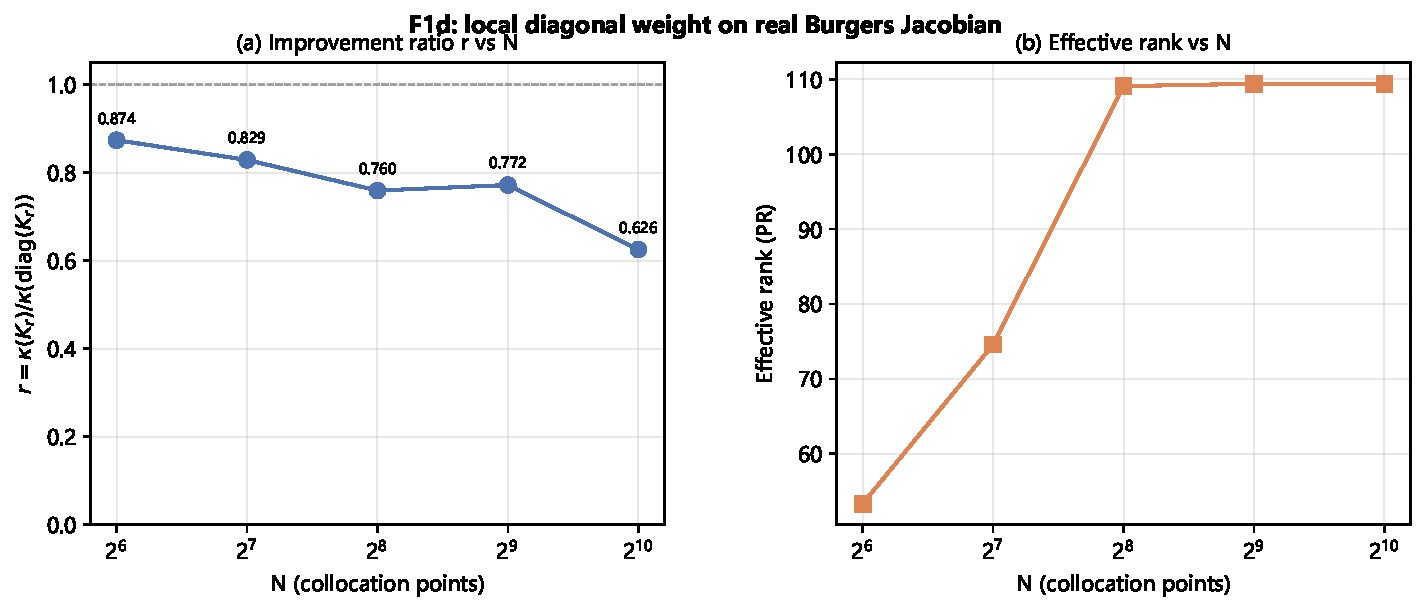
\includegraphics[width=0.92\textwidth]{fig_F1d_real_jacobian_en.pdf}
\caption{Experiment 4.2: $N$-scan on the real frozen Burgers Jacobian ($\nu=.005$, near-solution good basin). Left: improvement ratio $r=\kappa^*_{\rm diag}/\kappa(R(K_r))$ versus $N$; for $N=64$--$512$, $r\approx.76$--$.87$ (multi-start-found improvement 13\%--24\%); $N=1024$ excluded due to the double-precision limit. Right: the effective rank (PR) saturates at $\sim109$ as $N$ grows, indicating dominance of directional collinearity at the stiff end.}\label{fig:f1d}
\end{figure}

\begin{figure}[ht]\centering
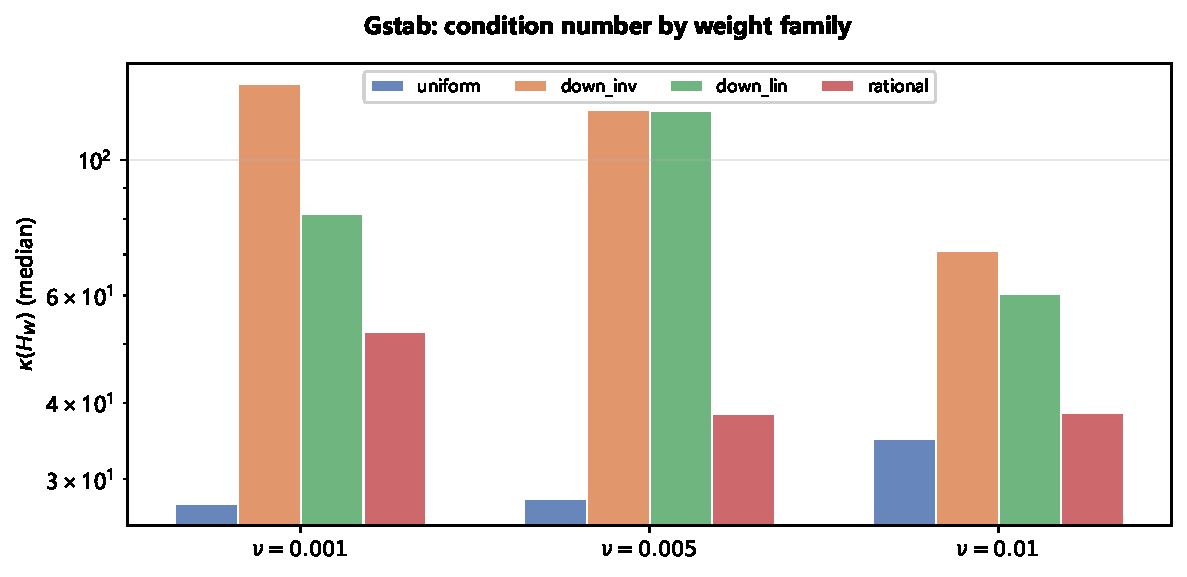
\includegraphics[width=0.85\textwidth]{fig_gstab_kappa_med_en.pdf}
\caption{Experiment 4.3: time median of the full-Hessian spectral-edge ratio $\kappa=\lambda_{\max}/|\lambda_{\min}|$ (algebraic-extremum convention, ARPACK/Lanczos edge estimate, Appendix~\ref{app:repro}) during training ($n=22/\nu$, 11 seeds $\times$ 2 clip settings). At low viscosities (.001/.005) the down-weighting families (down\_inv/down\_lin) worsen the spectral-edge ratio by 3--5$\times$; the rational up-weighting family shows no significant difference from uniform. The right-spectral-edge $\lambda_{\max}$ ordering agrees with the gradient-peak ordering (rational$\gg$uniform$>$down\_lin$>$down\_inv), but as described in \S\ref{sec:theta-down}, this scale difference is absorbed by normalization under Adam.}\label{fig:gstab}
\end{figure}

\begin{figure}[ht]\centering
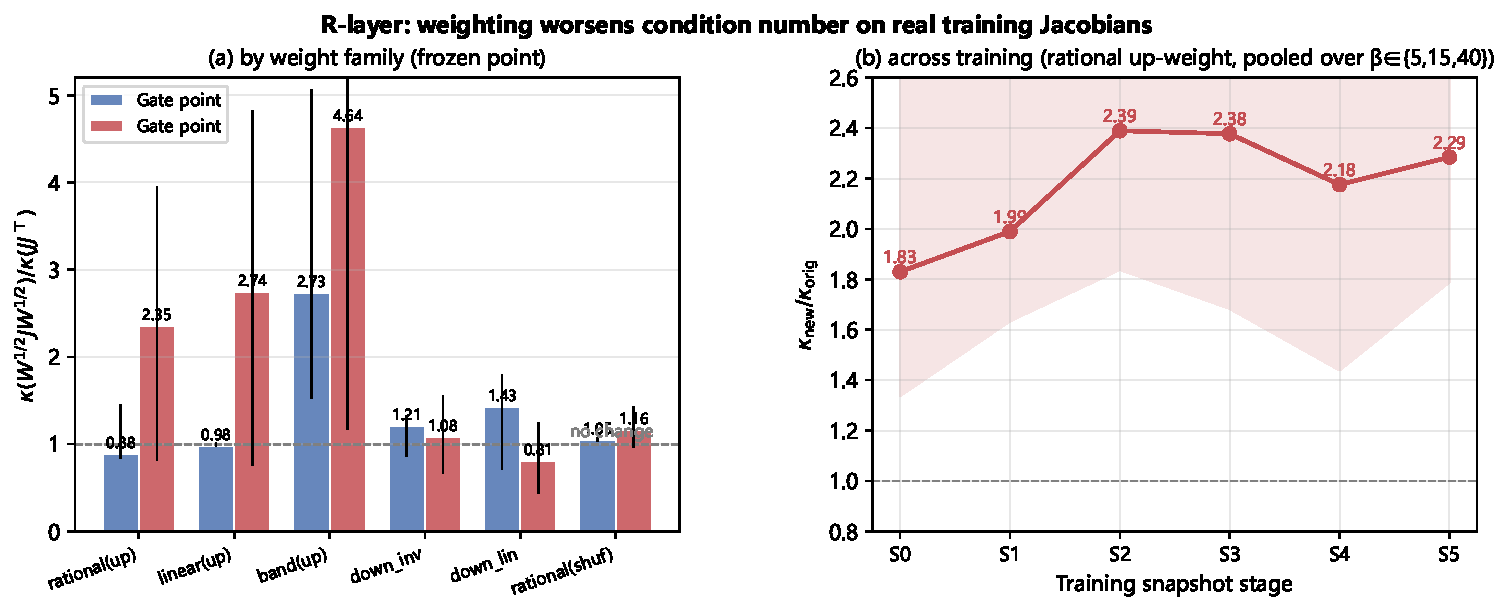
\includegraphics[width=0.95\textwidth]{fig_C2E3_kappa_train_en.pdf}
\caption{Experiment 4.4: ratio of the weighted to unweighted condition number $\kappa(W^{1/2}JW^{1/2})/\kappa(JJ^\top)$ on real training Jacobians. (a)~By weight family, at the Gate and convergence points (six fixed-weight families): up-weighting families worsen by $2.35$--$4.64\times$ at the convergence point; down-weighting families are near $1$ or slightly better; (b)~throughout training ($S_0$--$S_5$, rational up-weighting family, pooled over $\beta\in\{5,15,40\}$ with per-snapshot medians, applied statically per snapshot and not entering training, hence not violating the frozen-$W$ boundary): ratio median $1.83$--$2.39$, always $>1$. Note that this figure measures the frozen linearization $H_{\rm lin}$, unlike Experiment 4.3 which measures the full $H_{\rm lin}+H_{\rm nl}$, so down\_lin's $.81$ here (improvement) does not contradict Experiment 4.3's ``3--5$\times$ worsening.'' Dashed line $=1$ means no change.}\label{fig:c2e3}
\end{figure}

\FloatBarrier

\section{First-Order Level: Optimization-Dynamics Boundaries}\label{sec:theta}

This section studies the dynamical effects of spatial weighting after it enters the single-step update through the weighted gradient $g_\W=J^\top\W r$ (frozen or exogenously slowly-varying $\W$ convention; the online recomputation $\W(\theta)$ of Experiment 5.3 is an out-of-class empirical observation---see the Experiment 5.3 protocol statement, Table~\ref{tab:g1b}). The core questions are: \emph{can weighting select basins? Can it accelerate convergence inside good basins? What is the operating range of down-weighting?} Across the six weight families studied here, with $n=80$ paired experiments, we do not observe that weighting significantly improves the basin-entry probability (the uniform hit rate $.613$ is in fact higher than that of all weighted families); the observable effect of weighting is confined to convergence-speed modulation inside an already-entered refinable basin. The true role of down-weighting is that of a gradient-scale modulator (manifesting on this testbed as early-training scale stabilization; terminal-state benefits under spectral mismatch are in Section~\ref{sec:crosseqn}), not a means of escaping pseudo-solution basins. Note that zero-solution-set invariance (Proposition~\ref{prop:zero}) does not imply attraction-basin invariance (Remark~\ref{rem:attractor}), so ``weighting cannot select basins'' is a controlled empirical conclusion, not a universal negation. This section first gives the necessary definitions and the algebraic layer of Mechanism~A, then the directional criterion, and finally controlled experimental verification.

\subsection{Weighted Training Flow, Basins, and the Two Phases}\label{sec:theta-flow}

\begin{definition}[Weighted training flow, attraction basins, and the two phases]\label{def:flow-basin}
Fixing a weight function $w(\cdot;\beta)$ and an optimizer, the parameter iteration $\theta_{k+1}=\mathcal A(\theta_k;w)$ induces a discrete flow. For a stationary point $\theta_B^\star$, its attraction basin is $B_{\W}(\theta_B^\star)=\{\theta_0:\lim_k\Phi_k^w(\theta_0)=\theta_B^\star\}$; the \emph{true-solution basin} is $B(u^\star)=\{\theta_0:\liminf_k\|u_{\theta_k}-u^*\|_X<\rho_{\rm bas}\}$, where $\rho_{\rm bas}>0$ is the nonlinear local absorption radius (uncalibrated; we do not claim an $O(\nu^2)$ scaling). Good/pseudo-solution basins are a conditional classification at the end of Phase~0: falling into $B(u^\star)$ is a refinable basin, otherwise a pseudo-solution basin.

\textbf{The two phases and the Gate stop}: \emph{Phase~0 (basin selection)} fixes $\beta=1$ by default and applies a $\sigma$-bandwidth curriculum, aiming to land in the true-solution basin with entry probability $p_{entry}$; the \emph{Gate (gate stop-time)} performs a one-shot policy split using ground-truth-free training observables; \emph{Phase~1 (in-basin refinement)} fixes the already-entered basin and adjusts $\beta$ and the weight family for local convergence. Basin membership is determined by Phase~0 dynamics, and Phase~1 does not reselect a basin (at the protocol level); whether moving weighting (up- or down-weighting) forward into Phase~0 can change basin entry is precisely the object of Experiments 5.3/5.7, whose conclusion (\S\ref{sec:theta-down}) is an empirical result rather than a prior protocol assumption.
\end{definition}

\begin{remark}[Zero-solution-set invariance $\ne$ attraction-basin invariance]\label{rem:attractor}
The zero-residual set is an algebraic object, independent of $w$ (Proposition~\ref{prop:zero}); an attraction basin is a dynamical-systems object determined by the vector field $-\nabla L_\W$, whose geometry and measure change with $w$. The precise meaning of ``solution-preserving but optimization-changing'' is: the zero-residual set is invariant while the family of basins is reshaped.
\end{remark}

\subsection{Mechanism A: Gradient-Energy Redistribution Inside Refinable Basins}\label{sec:theta-mechA}

\noindent\emph{Positioning.} Mechanism~A (up-weighting allocates gradient energy to hard regions) is itself a folkloric observation in the PINN community; our increment is: under the above stratification, to strictly separate levels, give its weight-function-level deterministic conditions (C1/C2, always true for rational weights) and its data-distribution-level contrast-separability condition (C-Sep), and delineate its failure boundary. Mechanism~A is not listed as a contribution on its own; its value is to provide the algebraic basis for the subsequent directional criterion and the controlled tests of the down-weighting hypothesis.

Divide the collocation points into a shock band $S$ and a smooth band $O$ ($|S|=O(\nu)N$). We call the data \textbf{contrast-separable} (C-Sep) when the lowest contrast in the shock band is no lower than the highest contrast in the smooth band, i.e., when sorting by relative residual magnitude the two bands do not overlap at all; its probabilistic relaxation (C-Sep$^*$) requires only that the contrast distribution of the shock band first-order stochastically dominates that of the smooth band. C-Sep is the \emph{data-distribution} premise for ``up-weighting indeed adds more weight to hard regions'': the weight function knows only the contrast $t$, not the ``shock''; the bridge ``$t$ large $\Leftrightarrow$ hard region'' is paved by the training dynamics of Phase~0 and cannot be guaranteed by the weight function itself. Mechanism~A is stated in two layers.

\begin{proposition}[A0: nominal redistribution (certain at the weight-function level)]\label{prop:mechA0}
\emph{Weight-function level (deterministic)}: assume (C1)~$\partial_\beta w\ge0$; (C2)~$\partial_\beta w(t;\beta)$ is nondecreasing in $t$; (C2$'$)~the relative growth rate $\partial_\beta w/w$ is nondecreasing in $t$. For rational weights, $\partial_\beta w=t/(1+t)\in[0,1)$, $\partial_t(\partial_\beta w)=1/(1+t)^2>0$, $\partial_\beta w/w=t/(1+\beta t)$ and $\partial_t[\partial_\beta w/w]=(1+\beta t)^{-2}>0$, so C1/C2/C2$'$ hold for all $\beta\ge1,t\ge0$. \emph{Data-distribution level (contrast ordering)}: denote the contrasts on $S,O$ by $\{t_i\}$; the strict version (C-Sep) is $\min_{i\in S}t_i\ge\max_{i\in O}t_i$, and the probabilistic version (C-Sep$^*$) requires only that $t|_S$ first-order stochastically dominates $t|_O$. Then under strict C-Sep, $\partial_\beta\bar w_S\ge\partial_\beta\bar w_O\ge0$ (needing only C1/C2, \textbf{[certain]}); and $\bar w_S/\bar w_O$ is nondecreasing in $\beta$ (needing C2$'$; C1/C2 alone are insufficient---counterexample in the appendix, \textbf{[certain]}); under C-Sep$^*$, the monotonicity of C2 and the order preservation of first-order stochastic dominance \cite{Strassen1965} give $\mathbb E_S[\partial_\beta w]\ge\mathbb E_O[\partial_\beta w]$, so A0 holds \emph{in expectation} (\textbf{[certain]}, given the dominance assumption). When strict C-Sep is violated, the deviation of A0 is quantified by the inversion gap $\Delta=\max_{i\in O}t_i-\min_{i\in S}t_i$ and the mass of inverted points; the more severe the inversion, the more likely the nominal redistribution reverses in expectation.
\end{proposition}
\begin{proof}[Proof sketch] The complete proof is in Appendix~\ref{app:proof}.
The weight-function level follows directly from $\partial_\beta w\ge0$ nondecreasing in $t$. Data-distribution level: under strict C-Sep, every $t_i$ on $S$ is at least every $t_j$ on $O$; since $\partial_\beta w$ is nondecreasing, $\partial_\beta w(t_i)\ge\partial_\beta w(t_j)$, and averaging gives the result. The probabilistic version follows from order preservation of first-order stochastic dominance (Strassen's theorem): if $F_S\le F_O$ and $f$ is nondecreasing, then $\int f\,dF_S\ge\int f\,dF_O$. The inversion error comes from integration by parts: $\partial_\beta\bar w_S-\partial_\beta\bar w_O=-\int q'(t)(F_S-F_O)dt$, and the violating part comes only from the positive part $(F_S-F_O)_+$. The complete proof is in Appendix~\ref{app:proof}.
\end{proof}

\begin{proposition}[A1: realization of parameter-gradient energy (local, conditional)]\label{prop:mechA1}
On top of A0, add (C3)~\emph{in-band non-self-cancellation}: $\langle\partial_\beta g_S,g_S\rangle\ge0$ (the weighted sum of in-band row gradients $J_i$ does not cancel itself out as weights increase). Then $\partial_\beta\|g_S\|^2=2\langle\partial_\beta g_S,g_S\rangle\ge0$; whereas on the $O$ band, boundedness of $t$ and $\partial_\beta w$ gives only the upper bound $\partial_\beta\|g_O\|^2\le\varepsilon_O\|g_O\|^2$ ($\varepsilon_O:=2t_O^*(1+\eta_O\|g_O\|)$, $\eta_O$ the out-of-band non-self-cancellation constant, derivation in the appendix); no non-self-cancellation is assumed on the $O$ band, so no lower bound is claimed---its sign can be positive or negative, only controlled by the upper bound so as not to blow up. C3 is a pointwise measurable algebraic condition; Experiment 5.2 finds that it holds in good and bad basins alike (all $176$ probe records are positive)---Mechanism~A performs its energy redistribution in pseudo-solution basins as usual, and the reason it cannot correct basin membership lies not in C3 but in the acceleration direction being locked onto the in-basin stationary direction $d_B$ rather than the true-solution direction $d_*$ (see the reference-frame discussion below).
\end{proposition}
\begin{proof}[Proof sketch] The complete proof is in Appendix~\ref{app:proof}.
$\partial_\beta\|g_S\|^2=2\langle\partial_\beta g_S,g_S\rangle$, nonnegativity follows directly from C3. For the $O$ band, $\partial_\beta w\le1$ (rational weights) and boundedness of $t_O^*=\max_{i\in O}t_i$ give $\partial_\beta\|g_O\|^2\le2t_O^*(\|g_O\|^2+\eta_O\|g_O\|^3)$. The complete derivation is in Appendix~\ref{app:proof}.
\end{proof}

\noindent\emph{Computational intuition.} The algebraic essence of up-weighting being effective in hard regions is ``allocating more of the finite gradient energy to hard regions according to contrast,'' which is a deterministic identity at the weight-function level; but whether it is realized depends on the data distribution (C-Sep) and requires already being inside the correct basin (C3). Up-weighting is a refinement tool inside refinable basins, not a correction tool for pseudo-solution basins.

\subsection{The Directional Criterion and the Discrimination Boundary of the Alignment Angle}\label{sec:theta-align}

\begin{definition}[Two target directions and the alignment angle]\label{def:align}
Distinguish two target directions: the \emph{own-basin stationary-point direction} $d_B=\theta_B^\star-\theta$, where $\theta_B^\star$ is the stationary point of the basin currently occupied (defined as in \S\ref{sec:theta-flow}; inside a bad basin $\theta_B^\star$ is the pseudo-solution minimizer); and the \emph{true-solution direction} $d_*=\theta^*-\theta$, where $\theta^*$ is a representation parameter of the true solution, i.e., any parameter with $u_{\theta^*}=u^\star$. Inside good basins $d_B=d_*$; inside bad basins the two differ. For the descent direction $-g$ define the cosine ($\cos>0$ means descent heads toward the target):
\begin{equation}\label{eq:cos}
\cos\alpha(\beta;d)=-\frac{\langle g,d\rangle}{\|g\|\|d\|}\in[-1,1].
\end{equation}
\end{definition}

\begin{proposition}[First-order directional criterion for up-/down-weighting]\label{prop:align}
For gradient descent $\theta^+=\theta-\eta g$, the single-step change of the squared distance $D=\tfrac12\|\theta-\theta_B^\star\|^2$ to the target $d$ is
\begin{equation}\label{eq:step}
D^+-D=\eta\langle g,d\rangle+\tfrac{\eta^2}{2}\|g\|^2
=-\eta\|g\|\|d\|\cos\alpha+O(\eta^2).
\end{equation}
Under G-C local linearity, small step size ($\eta\lambda_{\max}\ll1$, the $\eta^2$ term negligible), and in-band quasi-uniformity (C3$'$, small coefficient of variation of contrast within the shock band): (i)~when $\cos\alpha_S>c_0>0$ (descent heads toward the target), increasing $\beta$ amplifies the alignment of $-g_S$ with $d$ and \emph{accelerates the approach} (a sufficient condition for up-weighting refinement in good basins); (ii)~when $\cos\alpha_S<-c_0<0$ (descent heads away from the target), increasing $\beta$ makes $\eta\langle g,d\rangle>0$---\emph{single-step expected departure, faster with larger $\beta$}; (iii)~down-weighting ($w_S<1$) scale-wise suppresses the gradient contribution of that direction---it is merely a local gradient-scale rebalancing and does not imply cross-basin escape. This criterion holds for \emph{arbitrary} target directions $d$; it is pure first-order geometry, independent of Burgers.
\end{proposition}
\begin{proof}[Proof sketch] The complete proof is in Appendix~\ref{app:proof}.
Eq.~\eqref{eq:step} follows directly from a Taylor expansion. Under C3$'$, $\partial_\beta g_S=\bar c_\beta g_S+v_S$, $\|v_S\|\le\varepsilon_S\bar c_\beta\|g_S\|$, so $\partial_\beta\langle g_S,d\rangle=\bar c_\beta\langle g_S,d\rangle+\langle v_S,d\rangle$, and when $|\cos\alpha_S|>\varepsilon_S$ the sign is determined by $\langle g_S,d\rangle$. The complete proof is in Appendix~\ref{app:proof}.
\end{proof}

\begin{remark}[The alignment angle cannot discriminate good from bad basins]\label{rem:align-emp}
Proposition~\ref{prop:align} requires only G-C local linearity and the existence of an in-basin target $d$. Substituting the two reference frames: in good basins $d_B=d_*$---the two frames coincide, and up-weighting accelerates along $d_B$, i.e., toward the true solution; in bad basins, accelerating along $d_B$ means moving \emph{away from the true solution} along $d_*$. Note that both target directions are \emph{oracle quantities}: $d_*$ presupposes the true solution $\theta^*$, and $d_B$ must be approximated offline by a long-trained converged solution in the same basin (Experiment 5.2 constructs it with the $\beta_{\rm ref}=20$ long-trained solution), so this criterion is an analysis tool, not a deployable online test. Experiment 5.2's offline measurements (frozen Gate point, $\beta=1$; data in \S\ref{sec:theta-exp}) show: for bad basins against $d_B$, the median $\cos\alpha_S$ is $+.0885$, all $18/18$ positive (range $[+.007,+.461]$); for good basins against $d_*$, the median $\cos\alpha_S$ is only $+.0047$, $24/26$ positive (range $[-.0045,+.594]$) (\textbf{[empirical: bad $n=18$, good $n=26$]}). In the same probe, the C3 inner product $\langle\partial_\beta g_S,g_S\rangle$ is positive in all $176$ records (including bad basins): Mechanism A's energy redistribution works as usual in pseudo-solution basins---what fails is not redistribution itself, but the fact that its acceleration direction is locked onto $d_B$. For both basin types the alignment angles to their respective target directions are predominantly positive, with good-basin medians even closer to zero---the sign distribution of $\cos\alpha_S$ has no separation power over basin quality; discriminating quality is the job of Gate/Experiment 6.1 (Section~\ref{sec:methods}).
\end{remark}

\subsection{The Operating Range of Down-Weighting}\label{sec:theta-down}

\paragraph{Basin entry: the down-weighting escape hypothesis is rejected by large-sample paired evidence.}
That PINNs converge to pseudo-solution basins with small training residual but physically wrong solutions, and that continuation/resampling/domain-shrinking help avoid pseudo-solutions, is itself established \cite{Rohrhofer2022,WangPseudo2026}; this paper claims neither first discovery of pseudo-solutions nor first circumvention. An early $n=3$ exploratory experiment observed that ``among pseudo-solution basins only down\_inv can escape,'' on which a \emph{spatial down-weighting escape} claim was once proposed. That claim is rejected under the $n=80$ paired Experiment 5.3 (Table~\ref{tab:g1b}): pairing by the same Phase~0 coarse solution (eliminating initialization confounds), the uniform refinable-basin hit rate $.613$ is in fact higher than that of all weighted families ($.388$--$.475$); the paired net-rescue counts are negative for all three families, and after Holm correction only down\_lin is significant ($p=.006$) (\textbf{[empirical $n=80$]}). So the facts as a whole do not support ``down-weighting improves basin entry,'' but we do not make the universal negation that down-weighting can never change basin membership under any circumstance.

\paragraph{Gradient scale: under Adam, clipping is redundant and down-weighting's scale is absorbed by normalization (Experiment 5.7, $n=20$ paired, no multiple-comparison correction).}
To separate the ``scale component'' from the ``direction component'' of down-weighting, we design the family$\times$clip-switch $2\times4$ factorial-design Experiment 5.7: under the same Phase~0 protocol, compare grad\_clip$=1$ (default) with grad\_clip$=0$ (off). Results: (i)~after switching clipping off, zero blow-ups (blown$=0$, including $\nu=.001$ and the up-weighting family rational, whose pre-clip gradient peak reaches $7\times10^2$; the matched Experiment 4.3 Stage-E configuration has measured median 721); (ii)~at $\nu=.005$ the clip switch shows no observed effect on basin-entry rate (four-family paired McNemar $p=1.00$, entry-rate differences all within $\pm.05$); (iii)~significant signals appear only at the stiffest end $\nu=.001$ with clipping on, where uniform significantly beats the two down-weighting families (vs down\_inv $p=.016$, vs down\_lin $p=.039$), reproducing Experiment 5.3; with clipping off, inter-family differences are insignificant (full statistics in \S\ref{sec:theta-exp}, Figure~\ref{fig:g1c}). Mechanism: Adam's second-moment normalization $\sqrt{\hat v_t}$ already adaptively absorbs the scale effect of the raw gradient norm; explicit L2 clipping and the suppression of $g_{\text{peak}}$ by spatial down-weighting do not transmit to the optimization trajectory under Adam (\textbf{[empirical $n=20$]}).

\paragraph{In-basin lr margin: linear down-weighting down\_lin raises the effective training ceiling (Experiment 5.8, $n=8$ paired, directional evidence).}
Starting from the Gate point (inside a good basin), run fixed-step Adam for 500 steps. The stable lr in the blow-up sense is extremely wide: for lr$\le.05$ no family blows up; at lr$=.1$ only rational (up-weighting) blows up at $50\%$, down-weighting families at $12.5\%$, uniform at $0\%$. But the \emph{effective training lr ceiling}, defined by the terminal $L_2<.06$ (good-basin threshold), shows that the down\_lin median $.002$ is higher than uniform's $.001$ (paired Wilcoxon exact two-sided $p=.0625$, asymptotic $\approx.043$; only $5$ of the $n=8$ pairs have nonzero differences---a consistent direction that does not reach $.05$ significance). Under looser thresholds $L_2<.1$ / $<.2$, down\_lin's advantage is more visible (median $.0035$ / $.005$, other families $.001$--$.002$; full statistics in \S\ref{sec:theta-exp}, Figure~\ref{fig:b1b}). Conclusion: after entering a good basin, linear down-weighting raises the median effective training lr ceiling by about a factor of two, but the effect is small, appears as only a marginal trend in the down\_lin family (exact $p=.0625$), and does not change basin entry (\textbf{[empirical $n=8$; seeds 10/15/20 excluded for having no good basin]}).

\paragraph{Fixed-step L-BFGS control: no significant terminal-state difference across the four families (Experiment 5.9, $n=5$--$8$, negative result, directional evidence).}
To test whether ``Adam normalization absorbs scale'' is the reason down-weighting yields no basin-entry benefit, we design a fixed-step L-BFGS control (\texttt{line\_search\_fn=None}, no Adam-style per-coordinate normalization; the secant matrix is constructed only from historical weighted gradients, within the admission class): Adam 200-step warm-up + L-BFGS 500 outer steps. At $\nu=.005$ ($n=8$) and $\nu=.001$ ($n=5$, other seeds have no good basin), the four families show no significant terminal-$L_2$ differences, with zero blow-ups in all configurations (full statistics in \S\ref{sec:theta-exp}). Conclusion: even with Adam normalization removed, spatial down-weighting produces no detectable terminal-state difference inside good basins---gradient scale is not the bottleneck of in-basin optimization (\textbf{[empirical]}).

\paragraph{Gradient curves: the geometric effect of down-weighting suppressing peaks is real ($n=8$; subsumed in Experiment 5.9).}
From the Gate point, lr$=10^{-3}$, recording the pre-clip $\|g\|_2$ every 50 steps: within 500 steps the ordering is stable---rational ($27$--$63$) $\gg$ uniform ($3$--$6$) $>$ down\_lin ($.2$--$.8$) $>$ down\_inv ($.1$--$.4$). Down-weighting's suppression of gradient scale is real and does not converge away over the run, but as stated above, this effect is absorbed by normalization under Adam and does not change terminal states under fixed-step L-BFGS either.

\medskip
\noindent\textbf{Summary.} Spatial down-weighting (especially linear down-weighting down\_lin) has a slight lr-margin stabilization effect after entering a good basin (median effective training lr ceiling doubled, exact two-sided $p=.0625$, asymptotic $\approx.043$---a marginal trend not reaching $.05$ significance), but its scale component is absorbed by Adam normalization and it does not change terminal states under fixed step sizes either; it does not help enter basins, does not escape pseudo-solutions, and is not a preconditioner. The operating window of down-weighting is strictly confined to the narrow region ``in-basin, linear down-weighting, lr margin.''

\subsection{Experimental Verification}\label{sec:theta-exp}

\noindent\textbf{Optimizer and admission-class statement.} For all main experiments in this section (Experiments 5.1/5.2, Experiment 5.3, Experiments 5.4/5.5/5.6, Experiment 6.1), both Phase~0 and Phase~1 use fixed-step Adam ($\beta_1=.9,\beta_2=.999$, no line search based on $L_\W$), which is an admitted algorithm of Definition~\ref{def:admit}, covered by Lemma~\ref{lem:linrec}. Experiment 4.3's Stage-B2 is a fixed-step L-BFGS control experiment (PyTorch \texttt{LBFGS}, without \texttt{line\_search\_fn} set, i.e., no Armijo backtracking; the secant matrix is constructed from historical weighted gradients---an indirect quantity within the information set $\mathcal I_k$, not reading $L_\W$), also within the admission class. This paper uses neither line-search L-BFGS nor any optimizer that directly reads $L_\W$.

\paragraph{Experiments 5.1/5.2: directional verification of Mechanism A (deterministic self-check at frozen points).}
Freezing the Gate point, same $\theta$ same $r$, only changing $\beta$: the shock-band gradient-energy share $\eta_{gate}$ is monotone in $\log\beta$; the frozen-point self-check script has Spearman rank correlation $+1$ at all four viscosities, and Experiment 5.1 leaves the direction unchanged across 7 configurations spanning width/depth/collocation (Figure~\ref{fig:r1g3}; full data in Appendix Table~\ref{tab:app-r1}). \emph{Direct C-Sep measurement}: at the same frozen point, compute the contrast $t=|r|/\mathrm{median}|r|$ on the shock band $S$ ($|x|<3\nu$) and the smooth band $O$; for $N=128$--$512$ the inter-band median ratio $\mathrm{median}(t_S)/\mathrm{median}(t_O)=38$--$45$ (the strict C-Sep ratio $\min(t_S)/\max(t_O)=0.72$--$8.88$; at $N=512$ the strict version fails but the median ratio still reaches $38$), i.e., the data premise of Mechanism~A empirically holds at stiff-end frozen points. Note the evidence level of Experiment 5.1: this is a rank-monotonicity self-check of the deterministic function $\beta\mapsto\eta_{gate}$ at \emph{the same frozen point} (mechanism verification)---as long as C1/C2 and C-Sep hold at that point it is identically $+1$; it is \emph{not} a cross-seed empirical statistic and constitutes no training-benefit evidence; its role is to verify that the algebraic layer of Propositions~\ref{prop:mechA0}/\ref{prop:mechA1} holds at measured frozen points. This monotonicity neither implies final convergence nor discriminates basin quality.

\paragraph{Experiment 5.2 alignment-angle probe: $\cos\alpha_S$ has no separation power over basin quality.}
The same Experiment 5.2 probe offline-measures the shock-band alignment angle $\cos\alpha_S=-\langle g_S,d\rangle/(\|g_S\|\|d\|)$ at frozen Gate points, with the target direction $d$ constructed from the same-basin $\beta_{\rm ref}=20$ long-trained converged solution (an offline oracle, not a ground-truth-free deployable quantity), totaling $11$ seeds $\times$ $4$ viscosities $\times$ $4$ $\beta$ levels, $176$ records. At $\beta=1$ ($\beta=3/10/40$ nearly identical): bad basins ($n=18$, against the own-basin pseudo-solution stationary direction $d_B$) have median $\cos\alpha_S$ $+.0885$, all $18/18$ positive (range $[+.007,+.461]$); good basins ($n=26$, against the true-solution direction $d_*$) have median $+.0047$, $24/26$ positive (range $[-.0045,+.594]$). The sign distributions of the alignment angles of the two basin types show no separation; this is the empirical source of the discrimination-boundary conclusion of Remark~\ref{rem:align-emp}.

\begin{figure}[ht]\centering
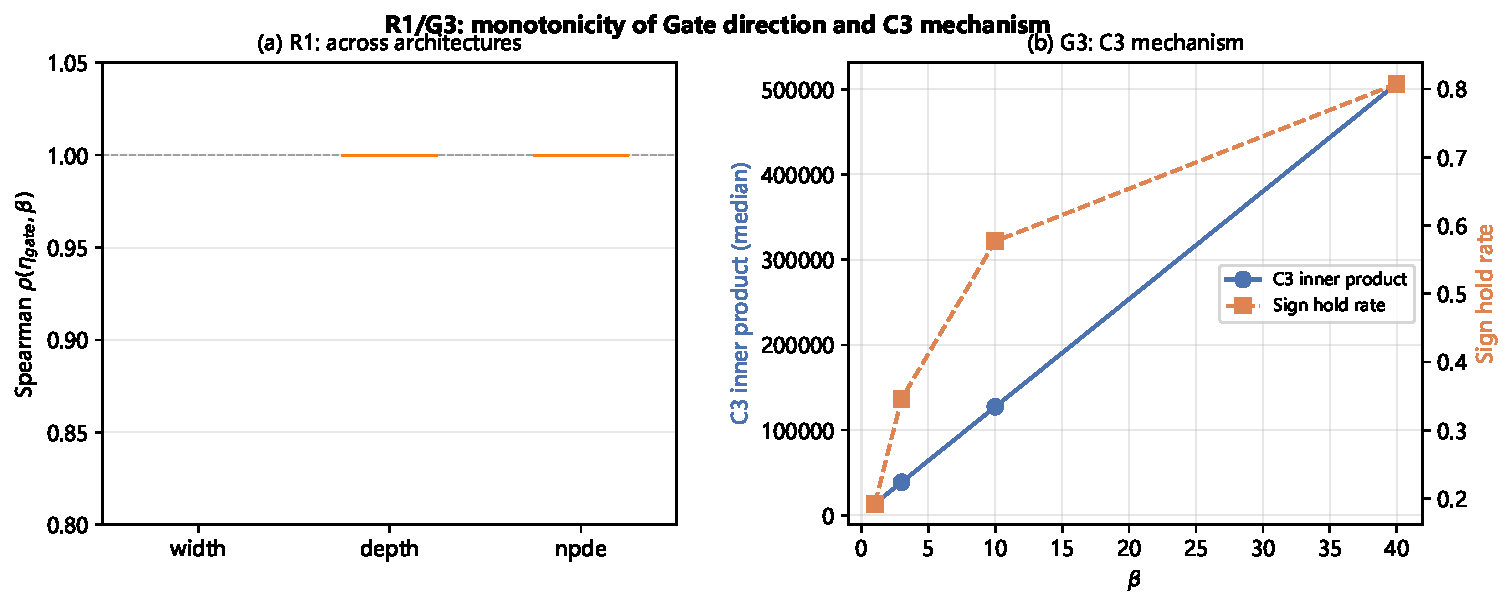
\includegraphics[width=0.92\textwidth]{fig_R1_G3_monotonicity_en.pdf}
\caption{Experiments 5.1/5.2: directional verification of Mechanism A. Left (Experiment 5.1): Spearman rank correlation of the Gate directional quantity $\eta_{gate}$ against $\beta$ across architectures (width/depth/collocation count), all $\rho_s=+1$ (deterministic self-check at frozen points, architecture-independent); right (Experiment 5.2): inside good basins, the median C3 inner product $\langle\partial_\beta g_S,g_S\rangle$ increases monotonically with $\beta$ ($1.4\times10^4\to5.1\times10^5$, blue, left axis; all $176$ probe records are positive, so the weak condition C3 holds pointwise at frozen Gate points); the attainment rate of the directional criterion's sign condition (fraction of configurations with $\cos\alpha_S>\varepsilon_S$, orange, right axis) rises from $.19$ to $.81$ as $\beta$ increases ($\varepsilon_S$ decreases with $\beta$, strengthening C3$'$).}\label{fig:r1g3}
\end{figure}
\paragraph{Experiment 5.3: basin entry and the down-weighting hypothesis test ($n=80$ paired).}
To study the effect of weights on basin \emph{entry}, this experiment moves the weight families forward into Phase~0 and recomputes $\W=\W(r(\theta))$ online: under the same $(\nu,\text{seed})$, the four families (uniform reuses the G1 cache; down\_inv/down\_lin/rational each at $\beta=10$) independently run Phase~0's $K=4$ multi-start selection (the $K=4$ starts are Phase~0 coarse solutions each retrained independently under 4 consecutive sub-seeds $s,s{+}1,s{+}2,s{+}3$ of the same $(\nu,\text{seed})$: fresh initializations, not restarts of a single trajectory; base seeds are spaced by 5 so sub-seed blocks do not overlap; cross-family pairs share the same sub-seeds, so the initialization directions are identical and only the weight family differs), and we compare the four families' hit rates of the Phase~0-final $L_2$ falling into the true-solution neighborhood (absolute threshold $L_2<.06$, family-independent) with same-seed paired McNemar tests. \emph{Protocol statement}: when weights are moved forward into Phase~0, the contrast field $t=|r|/\mathrm{median}|r|$ is recomputed online during training ($\W=\W(\theta)$)---an \emph{exploratory design} beyond Principle~II's frozen-$\W$ admission class. This online-recomputation design is also how practitioners deploy adaptive weights; its negative result probes the pre-Gate basin-entry boundary and complements, rather than conflicts with, Principle~II's conclusions for frozen $\W$ after the Gate. Principle~II's strict conclusions cover only Phase~1 refinement with frozen $\W$ after the Gate. The four families' hit rates and paired-test statistics are in Table~\ref{tab:g1b}.

\begin{table}[ht]\centering\small\renewcommand{\arraystretch}{1.2}\setlength{\tabcolsep}{3.5pt}
\begin{tabular}{lccccc}
\toprule
Weight family & Hit rate & Paired diff.\ (uniform$-$family) & 95\% CI$^\dagger$ & McNemar $p$ & Holm-corrected$^\ddagger$\\
\midrule
uniform & $.613$ & -- & -- & -- & --\\
rational & $.463$ & $+.150$ & $[+.003,+.297]$ & $.065$ & n.s.\\
down\_inv & $.475$ & $+.138$ & $[+.015,+.260]$ & $.043$ & n.s.\\
down\_lin & $.388$ & $+.225$ & $[+.086,+.364]$ & $.002$ & $p=.006$ (significant)\\
\bottomrule
\end{tabular}
\caption{Experiment 5.3: $n=80$ paired (4$\nu$ $\times$ 20 seeds, K=4 selection convention); refinable-basin hit rates of the weight families. The paired difference is the uniform hit rate minus the weighted family's (positive means uniform is better). Net rescue is negative for all three families. $^\dagger$95\% CIs are per-test (no multiple-comparison correction); all three families' CIs are entirely positive (highly consistent direction---uniform's hit rate exceeds every weighted family's), which is stronger directional-consistency evidence than any single significant test; $^\ddagger$after Holm correction (3 comparisons, familywise error control) only down\_lin is significant ($p=.006$); down\_inv and rational have consistent point-estimate directions but corrected $p>.05$. Stratified by $\nu$: the difference is largest at low viscosity (.001) (paired diff.\ $+.25$--$.35$), and the direction is inconsistent at the transitional viscosity (.01). Conclusion: under $n=80$ pairing we do not observe that down-weighting significantly raises the basin-entry probability; uniform's hit rate is in fact higher than all weighted families'; no universal negation is made.}\label{tab:g1b}
\end{table}

\noindent\emph{Threshold robustness (N6)}: perturbing the good-basin threshold $\tau$ within $[.03,.08]$ and recomputing the paired McNemar, down\_lin remains significant after Holm correction for $\tau\in[.05,.08]$ ($p=.001$--$.032$); at $\tau=.03/.04$ the smallest family has only $18/80$ good-basin samples, so the test lacks power; the main conclusion is robust over the usual threshold range.

\paragraph{Experiments 5.4/5.5/5.6: empirical observations on up-weighting strength inside refinable basins ($n=11$ full set, descriptive).}
At the thin-shock end there is a post-hoc optimal $\beta$ (per-seed optimal $\beta^*$ medians $1/5/20/10$ across Experiment 5.4's $\nu=.001/.003/.005/.01$, and $8/1/3$ across Experiment 5.5's $\nu=.005/.1/.5$), but the per-seed spread is large ($1$--$100$), non-monotone in viscosity, and the three fixed strengths' terminal intervals overlap with no consistent ordering (Figure~\ref{fig:e1heat}; per-cell full data in Appendix Tables~\ref{tab:app-e1}, \ref{tab:app-r2}); at $\nu=.001$, $\beta\ge5$ all collapse to the same failure state (shown as the deep-red cells with cell-median $\approx.573$ in the heatmap; excluded from the fixed-strength comparison, retained in the $g_{\rm post}$ statistics below). At the smooth end the curves are nearly flat and gains fall to the error floor. The Experiment 5.6 degeneracy scan (1584-run) shows that the mechanistic gain is concentrated in the in-shock-band error of the MLP backbone (per-seed optimal median gain about $10.4/3.9$ at $\nu=.01/.03$; $4.43/1.40$ under the global-$L_2$ convention); at the smooth end the absolute error enters the $10^{-6}$ floor, the C-Sep partition loses its S/O semantics at $\nu\ge.3$, and relative gains are no longer interpreted as physical benefits; the fixed high-bandwidth Hi representer is clearly mismatched relative to MLP/Match at $\nu\ge.3$. The post-hoc optimal $\beta$ is only a descriptive achievable upper bound: over Experiment 5.4's thin-shock-end $n=44$ cells ($4$ viscosities $\times$ $11$ seeds, including failure-state cells), the post-hoc optimal relative gain $g_{\rm post}=\big(L_2(\beta{=}1)-\min_\beta L_2\big)\big/L_2(\beta{=}1)$ has median only $.08$, IQR $[0,.59]$, range $[0,.97]$, and $\beta^*$ is non-monotone in $\nu$---it does not constitute a deployable strategy, and a single-point $\beta^*(\nu)$ is not recommended.

\paragraph{Experiment 5.7: clip-switch factor ($n=20$ paired, separating scale and direction components).}
Family$\times$clip-switch $2\times4$ factorial design. With clipping off, zero blow-ups (including $\nu=.001$, rational with pre-clip peak $7\times10^2$); at $\nu=.005$ no effect of the clip switch on basin entry is observed (four families $p=1.00$); significant signals appear only at $\nu=.001$ with clipping on, uniform beating the two down-weighting families ($p=.016$/.039), reproducing Experiment 5.3. Adam's second-moment normalization has already absorbed the gradient scale; explicit clipping and down-weighting's suppression of $g_{\text{peak}}$ do not transmit to the optimization trajectory (\textbf{[empirical $n=20$]}; Figure~\ref{fig:g1c}).

\begin{figure}[ht]\centering
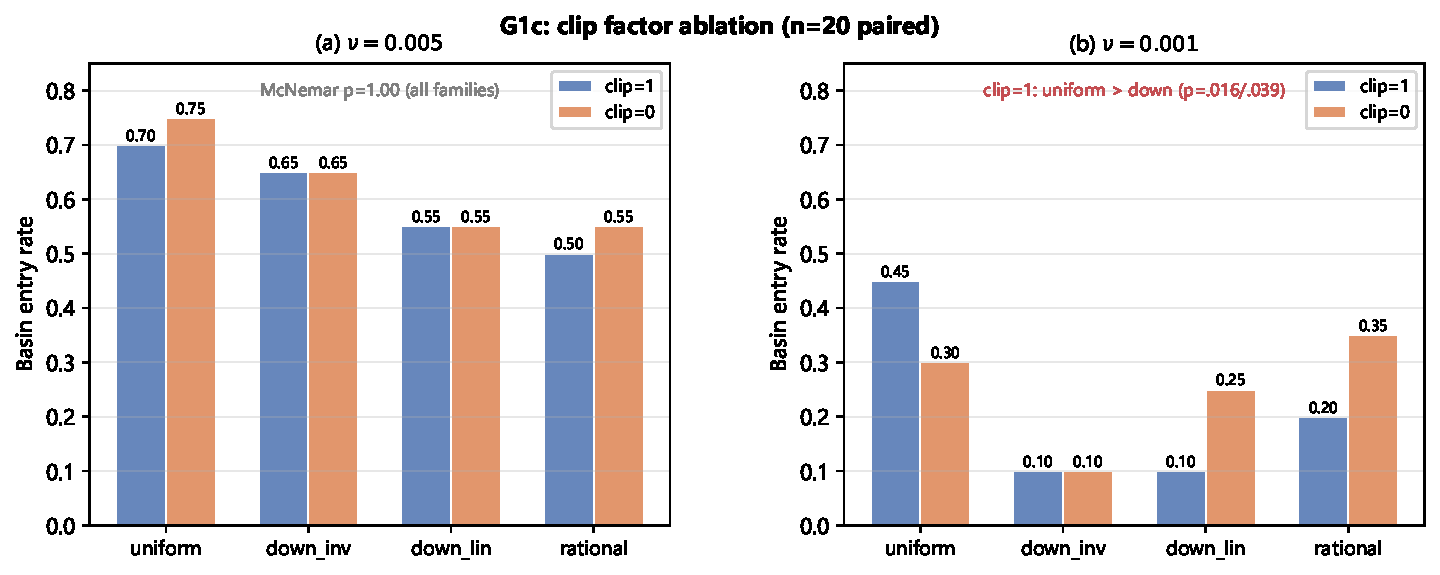
\includegraphics[width=0.92\textwidth]{fig_G1c_clip_en.pdf}
\caption{Experiment 5.7: clip-switch factorial ablation ($n=20$ paired, K=4 selection convention). Left: $\nu=.005$, no observed effect of the clip switch on basin-entry rate (four-family paired McNemar $p=1.00$); right: $\nu=.001$, with clipping on uniform significantly beats the two down-weighting families ($p=.016$/.039); with clipping off inter-family differences are insignificant. Zero blow-ups with clipping off.}\label{fig:g1c}
\end{figure}

\begin{figure}[ht]\centering
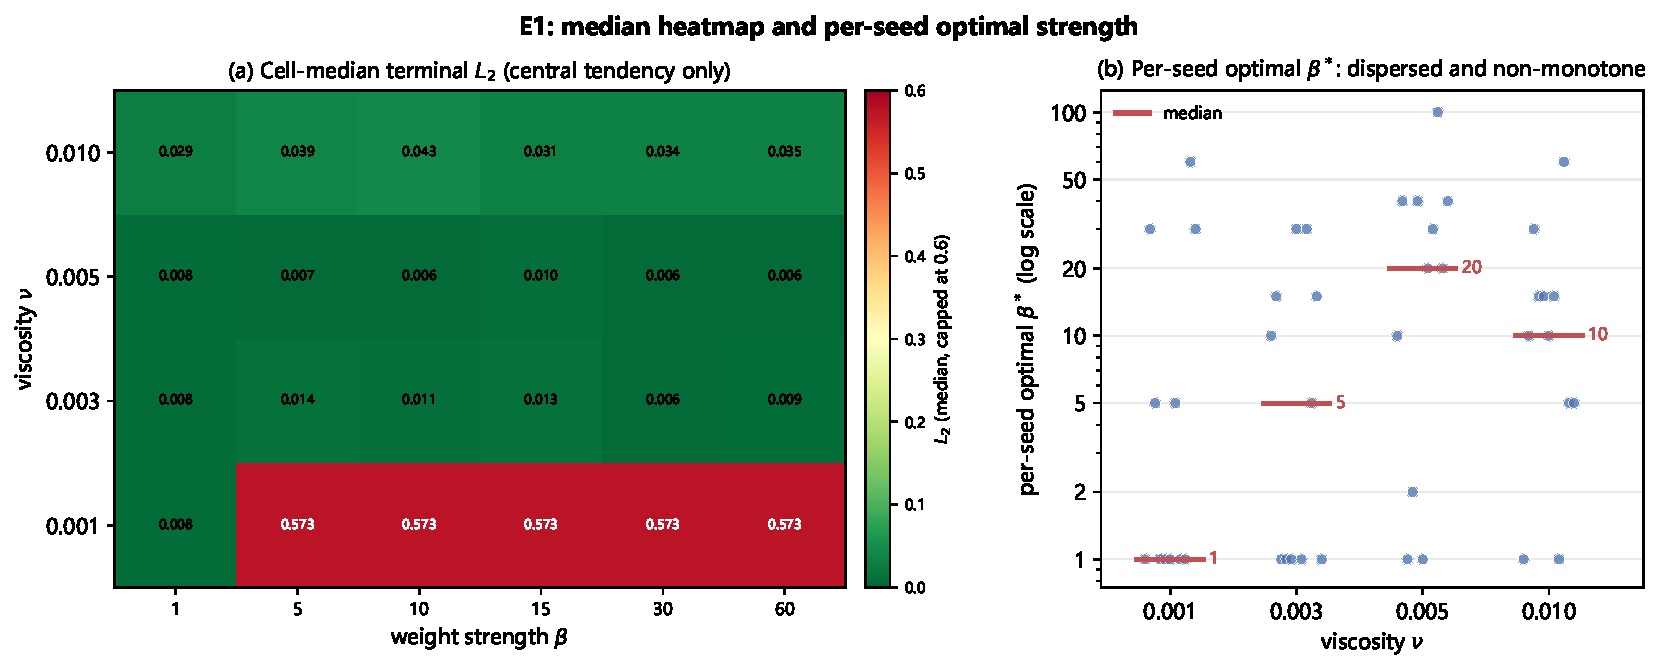
\includegraphics[width=0.98\textwidth]{fig_E1_beta_nu_heatmap_en.pdf}
\caption{Experiment 5.4: left, cell-median terminal $L_2$ ($n=11$, showing only the cross-seed central tendency) versus weighting strength $\beta$ and viscosity $\nu$; right, the distribution of per-seed optimal $\beta^*$ (medians $1/5/20/10$ across viscosities, overall median $10$, range $[1,100]$). A post-hoc optimal $\beta$ exists at the thin-shock end, but the per-seed values are widely dispersed and non-monotone in viscosity; the cell-median minimizer and the median per-seed $\beta^*$ need not coincide, and this figure is not used to identify a deployable strategy. At the high-viscosity end the curves are nearly flat and relative gains fall to the error floor. The left panel shows only the six $\beta$ values common to all four viscosities (the denser grid at $\nu=.005$ is listed in Appendix Table~\ref{tab:app-e1}); the deep-red cells at $\nu=.001$, $\beta\ge5$ are the single failure state to which all seeds collapse (cell-median $\approx.573$).}\label{fig:e1heat}
\end{figure}

\paragraph{Experiment 5.8/5.9: in-basin lr margin and optimizer controls.}
\emph{Experiment 5.8 ($n=8$)}: fixed-step Adam from the Gate point, lr grid $5\times10^{-4}$--$10^{-1}$. The stable lr in the blow-up sense is extremely wide (none blow up for $\le.05$), but the effective training lr ceiling defined by $L_2<.06$: down\_lin median $.002$ is higher than uniform $.001$ (paired Wilcoxon exact two-sided $p=.0625$, asymptotic $\approx.043$, a consistent direction not reaching $.05$ significance), down\_inv shows a trend ($p=.180$), rational is actually lower ($p=.109$). The down\_inv and rational pairs, and all Experiment 5.9 $p$ values below, use the normal asymptotic approximation (only $2$--$5$ nonzero paired differences, so exact enumeration is not applicable). Linear down-weighting doubles the median effective lr ceiling, but the effect is small, appears only as a marginal trend in down\_lin, and does not change basin entry (Figure~\ref{fig:b1b}).

\emph{Experiment 5.9 (fixed-step L-BFGS control)}: Adam 200-step warm-up + L-BFGS 500 outer steps (\texttt{line\_search\_fn=None}, within the admission class). At $\nu=.005$ ($n=8$), four families' terminal $L_2$ paired $p=.069$--$.161$ (no significant difference); at $\nu=.001$ ($n=5$), $p=.345$--$.686$. Even with Adam normalization removed, down-weighting produces no detectable terminal-state difference inside good basins---gradient scale is not the bottleneck of in-basin optimization.

\emph{Gradient-curve observation ($n=8$)}: within 500 steps the $\|g\|_2$ ordering is stable: rational $\gg$ uniform $>$ down\_lin $>$ down\_inv; down-weighting's peak-suppression geometric effect is real but does not change terminal states. The joint conclusion of the three is in \S\ref{sec:theta-down}.

\begin{figure}[ht]\centering
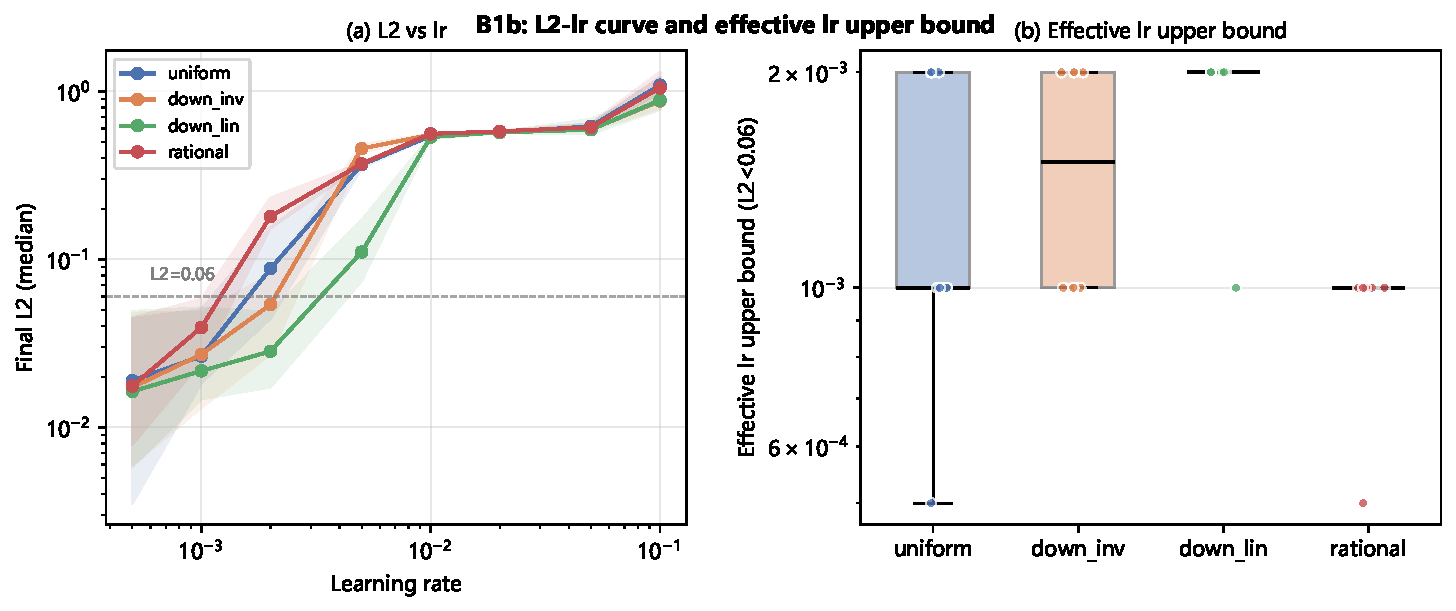
\includegraphics[width=0.92\textwidth]{fig_B1b_lr_curve_en.pdf}
\caption{Experiment 5.8: in-basin lr margin ($n=8$ paired, fixed-step Adam 500 steps from the Gate point). Left: terminal $L_2$ versus lr (median$\pm$IQR); for lr$\ge.01$ all four families plateau (leaving the good basin); the dashed line is the good-basin threshold $L_2=.06$; right: box plot of the effective training lr ceiling defined by $L_2<.06$---linear down-weighting down\_lin median $.002$ is higher than uniform $.001$ (paired Wilcoxon exact two-sided $p=.0625$, asymptotic $\approx.043$, a marginal trend with consistent direction not reaching $.05$ significance).}\label{fig:b1b}
\end{figure}

\noindent\textbf{Three empirical facts together outline the ``operating window'' of spatial weighting at the first-order level: an already-entered refinable basin $\times$ the presence of local stiffness contrast.} Across the six weight families studied here with $n=80$ pairing, outside the window---in pseudo-solution basins or on already-smooth problems---no significant basin-entry improvement from spatial weighting is observed, nor any systematic benefit. This is a controlled empirical conclusion and does not rule out effects of other weight families or adaptive strategies on basin selection.

\FloatBarrier

\section{Methodological Boundary of Ground-Truth-Free Discrimination}\label{sec:methods}

At deployment the two-phase pipeline is not allowed to use the ground truth, so the Gate stop-time can only rely on training observables. This section first gives the form of the Gate, then uses identifiability analysis to explain ``why residual/loss self-evaluation scalars are insufficient and what spatial-structure quantities are needed,'' and finally verifies with Experiment 6.1.

\subsection{The Gate Stop-Time and Two Kinds of Decisions}\label{sec:gate}

\begin{definition}[Gate stop-time and Gate-A/Gate-B]\label{def:gateAB}
The Gate is a \emph{one-shot} policy selector at the end of Phase~0, whose inputs are training observables $Z_k$ (no ground truth). \textbf{Gate-A} (deterministic trigger rule, operational definition): simultaneously (A-i)~the relative loss-decrease rate within the training window falls below a threshold and the gradient norm enters a plateau; (A-ii)~the frozen probe's $\eta_{gate}$ is monotone in $\beta$ (the A0/A1 aggregation of Mechanism~A holds); (A-iii)~the coarse solutions of the three representers (Hi/Match/MLP, see \S\ref{sec:theta-exp}) agree outside the shock band. The simultaneous holding of the three stipulates procedurally ``when to switch into Phase~1''---it is the design and stop-time definition of the Gate, \emph{not} a mathematical sufficient condition on ``objective basin quality'': the three measure training state and representation consistency, and the genuineness of the basin is still judged post hoc by whether Phase~1 can refine to the true solution. \textbf{Gate-B} (empirical, high-probability): when Gate-A is not fully decidable, a multivariate discriminator $\mathcal G_B(Z)$ estimates basin membership, with its sensitivity, specificity, and leave-one-out overall accuracy estimated by cross-viscosity leave-one-out experiments. Gate-B is a \emph{one-shot split}: on a bad verdict, restart with multi-start (no down-weighting escape); on a good verdict, enter Phase~1 and do not switch midway. In this paper Gate-B's leave-one-out performance serves only as \emph{feasibility evidence} (the samples cover only the measured viscosity grid of 1D steady Burgers), not a cross-equation deployment promise.
\end{definition}

\begin{remark}[Why training-loss self-evaluation cannot select basins]\label{rem:noground}
Pseudo-solution basins are likewise local minima, and their training loss can be driven down to levels comparable to refinable basins, so ``small training loss'' does not imply ``good basin''; Proposition~\ref{prop:bayes} will show that fixed single projections of the residual/loss self-evaluation type degenerate to chance level when the two classes' marginal distributions fully overlap, and are bounded by that scalar's Bayes error and the threshold-class restriction under partial overlap; the Gate must introduce spatial-structure quantities not equivalent to residual self-evaluation, or cross-validation across representers.
\end{remark}

\subsection{Identifiability: Bayes Error of Fixed Single-Projection Scalars and a Four-Point Counterexample}\label{sec:open}

\begin{proposition}[Identifiability lower bound for fixed single-projection scalar dictionaries (conditional)]\label{prop:bayes}
(i)~\textbf{Bayes lower bound}: for any discriminator $\mathcal G$, $\mathrm{Err}(\mathcal G)\ge\mathrm{Err}_B=\tfrac12\int\min(p_G,p_B)\,dZ$ (equal priors); only when the two class-conditional distributions are separable almost everywhere in $Z$ is $\mathrm{Err}_B=0$.
(ii)~\textbf{Identifiability lower bound for fixed-projection-family scalars (conditional)}: if the discriminator is only allowed to use scalars from a fixed projection family $\{t^\top z\}$ (typical examples are residual/loss self-evaluation quantities, such as the naive training loss and naive shock-band error; quantities carrying spatial-contrast structure are not covered by this item), then by the Cram\'er--Wold theorem this family cannot distinguish two classes with identical marginal distributions; denote the conditional densities of the two classes on such a scalar by $p_G,p_B$. Then: (a)~without restriction on the decision form, the optimal error rate on that scalar is its Bayes error $\mathrm{Err}_B(z)=\tfrac12\int\min(p_G,p_B)\,dz$ (overlap integral), which equals the chance level $\tfrac12$ under \emph{complete overlap} ($p_G=p_B$ almost everywhere), and can be strictly less than $\tfrac12$ under \emph{partial overlap}---hence ``distribution overlap'' itself does \emph{not} imply a chance-level lower bound; only ``complete overlap (identical marginals)'' does; (b)~if further restricted to the \emph{threshold rules} of ``comparing this scalar with a single fixed threshold'' (restricted class), the optimal error rate $\mathrm{Err}_{\rm thr}^*$ generally satisfies $\mathrm{Err}_{\rm thr}^*\ge\mathrm{Err}_B(z)$, with equality if and only if the likelihood ratio $p_B/p_G$ is monotone in the scalar; when the likelihood ratio is non-monotone (e.g., one class bimodal), every single-threshold rule is strictly suboptimal. This conclusion is conditional---if some scalar makes the two classes approximately separable, both $\mathrm{Err}_B$ and $\mathrm{Err}_{\rm thr}^*$ can be close to zero, so we do not claim that every scalar is useless in all cases.
(iii)~\textbf{Four-point counterexample (coinciding centroids; the fixed projection family cannot exactly separate)}: take the four points $G=\{(-\tfrac12,-\tfrac12),(\tfrac12,\tfrac12)\}$, $B=\{(-\tfrac12,\tfrac12),(\tfrac12,-\tfrac12)\}$ (textbook XOR). The two class centroids coincide at the origin, and every affine-linear function has the same mean on both classes, so \emph{no zero-error affine-linear separator exists}; the minimum error rate of all affine threshold rules (minimized over $f$ and the threshold) is $\tfrac14$ (e.g., take $f(z)=z_1+z_2$: values $\{\pm1\}$ on $G$, identically $0$ on $B$, optimal threshold error $\tfrac14$; in the single-coordinate degenerate case $ab=0$ the two classes' value multisets are identical and the error is exactly $\tfrac12$). Note that the two classes' marginals on a single scalar \emph{are not necessarily} completely overlapping---the above $f(z)=z_1+z_2$ has different marginal distributions and achieves error $\tfrac14$, so one cannot infer from the indiscriminability of single coordinates that ``every single-scalar discrimination is exactly at chance level''; the correct conclusion is ``exact (zero-error) separation is impossible.'' One must introduce the interaction feature $q=z_1z_2$ (or any nonlinear discriminator) to reach zero error. An $n=400$ \emph{synthetic four-point probe} (not Experiment 6.1 real samples, mechanism illustration only) reproduces the same boundary: single-coordinate AUC $=.542$, naive \emph{purely linear} two-coordinate AUC $=.566$ (near chance level), and adding the structural interaction $z_1z_2$ raises the AUC to $1.000$.
\end{proposition}
\begin{proof}[Proof sketch] The complete proof is in Appendix~\ref{app:proof}.
(i) Directly from the definition of the Bayes error. (ii)(a) From $\mathrm{Err}_B(z)=\tfrac12\int\min(p_G,p_B)dz$: when $p_G=p_B$, $\min=p_G$ and the integral is $1/2$; under partial overlap, $\min<p_G$ outside the overlap region and the integral is $<1/2$. (ii)(b) The optimal error rate of threshold rules is the minimum over the restricted class, and the minimum over a restricted class $\ge$ the minimum over the unrestricted class (the Bayes error); equality holds if and only if the Bayes rule itself belongs to the threshold class, i.e., the likelihood ratio is monotone. (iii) Direct verification: for any affine-linear function $f(z)=az_1+bz_2+c$, its two values on $G$ are $c-(a+b)/2$ and $c+(a+b)/2$, and on $B$ are $c+(-a+b)/2$ and $c+(a-b)/2$. Both class means equal $c$ (coinciding centroids), so the mean difference is zero. But the two classes' marginal distributions are \emph{not necessarily} identical: with $a=b=1$, $c=0$, the values on $G$ are $\{\pm1\}$ and on $B$ identically $0$, with optimal threshold error $1/4$. In general, the minimum error of all affine threshold rules is $1/4$: zero error is impossible (both class means equal $c$, and strict separation would require the two class means to lie on opposite sides of the threshold---contradiction); the error rate is an integer multiple of $1/4$ (each of the four points carries mass $1/4$), and $f=z_1+z_2$ attains $1/4$; in the single-coordinate degenerate case $ab=0$ the two classes' value multisets are identical and the error is exactly $1/2$. The interaction $q=z_1z_2$ equals $+1/4$ on $G$ and $-1/4$ on $B$---completely separable, achieving zero error. The complete proof is in Appendix~\ref{app:proof}.
\end{proof}

\begin{remark}[Scope and concurrent work]\label{rem:musah}
That a single aggregated scalar (training residual) cannot reliably select among candidate solutions is a general phenomenon recently confirmed independently and systematically: Musah \cite{Musah2026} observed in multi-field constrained systems, with extensive pairing across multiple architectures, the high-frequency reversal that ``candidates with lower residual are in fact worse solutions,'' and proposed lexicographic admissibility gating in which independent checks---structural identities, boundary traces, solvability integrals---must each pass before residuals may be compared. This paper \emph{concedes} that general observation and its systematic evidence in ranking multi-field soft/hard-constraint models; the increment of Proposition~\ref{prop:bayes} is: in the specific context of \emph{one-shot splitting of good/bad basins under spatial weighting}, to give a conditional formulation of the chance-level lower bound for fixed single projections of the residual/loss self-evaluation type and a rigorous four-point counterexample, and to point out that the way out is a structural quantity not equivalent to residual self-evaluation (the gradient-energy--contrast quantity of Experiment 6.1), not yet another residual threshold.
\end{remark}

\noindent\emph{Computational intuition.} Pseudo-solution basins are likewise local minima whose training loss can also be driven very low, so thresholds on residual/loss self-evaluation scalars such as the training loss alone cannot reliably judge whether the right basin was entered; at ground-truth-free deployment one must introduce quantities not equivalent to residual self-evaluation that carry spatial-contrast structure (e.g., the gradient-energy--contrast $g_et$), or cross-validation across representers---this is exactly the design basis of Gate-B. It must be emphasized that this conclusion does not cover scalars that themselves carry spatial structure, and that structural quantities can only judge ``success/failure of the current starting point,'' not ``whether a good basin exists'' (see Experiment 6.1).

\subsection{Experiment 6.1: Feasibility Evidence for Structural Quantities ($n=80$)}\label{sec:g2}

$n=80$ cross-viscosity configurations (the Cartesian product of $\nu\in\{.01,.005,.003,.001\}$ and $20$ equally spaced seeds), each configuration retaining $K=4$ multi-starts at the end of Phase~0 (construction in the Experiment 5.3 protocol paragraph of \S\ref{sec:theta-exp}). The \emph{oracle label} takes, among the $4$ starts, the one with the smallest true-solution $L_2$ at the end of Phase~0, marking whether the configuration \emph{has} a refinable basin: good $49$/bad $31$, existence rate $.613$. This $49/80$ and the uniform hit rate $49/80$ reported by Experiment 5.3 are \emph{the same statistic, not a numerical coincidence of two independent measurements}: both use exactly the same $(\nu,\text{seed})$ grid, $K=4$ multi-start truth-based selection, Phase~0-final $L_2$, and the same threshold $.06$; per-configuration labels agree $80/80$, and $L_2$ differs by at most $5\times10^{-7}$, so the two serve as mutual reproduction-consistency checks (rather than mutually independent evidence). The \emph{deployment (proxy) label} simulates ground-truth-free deployment: using the late-stage mean training loss---legitimately available at the Gate point but containing no ground truth---as proxy, select $1$ start from the same $K=4$ pool, then label post hoc with \emph{that start's} Phase~0-final true-solution $L_2$: good $14$/bad $66$. \textbf{Note on positive-class size}: under the proxy label the true good-basin positive class (post-hoc truly-good proxy-selected starts) has only $14/80$; the AUC and classification metrics below are all interpreted under this small positive class.

\emph{Discrimination performance (proxy selection convention, leave-one-out LOO)}: reported in three layers. (i)~\emph{Training-process quantities} (training loss, loss variance and slope, gradient norm, weighted mean, focusedness, etc., $7$ in total) have median AUC only $.51$ (range $.50$--$.59$, near chance level, corresponding to the overlap condition of Proposition~\ref{prop:bayes}(ii)); (ii)~the \emph{independent-grid aggregated residual} $r_{\rm resid}=\sqrt{\operatorname{mean}(r^2)}$ (unweighted PDE residual RMS on a fixed $2048$ dense grid) has proxy-convention AUC $.84$---it can validate ``whether the currently selected start works,'' but for ``whether a good basin exists'' (oracle existence convention) it drops to $.51$ (chance level): aggregated residual scalars can only do post-hoc acceptance; discovering good basins elsewhere requires multi-start or spatial-structure quantities; (iii)~\emph{spatial-structure quantities} are markedly higher (peak ratio $.95$, in-band mass $.90$, absolute peak $.89$, gradient-energy--contrast $g_et$ AUC $.971$; oracle-existence convention $.63$--$.70$; Figure~\ref{fig:g2auc}). Among them, $g_{et}$ (script variable \texttt{grad\_energy\_ratio}) has a closed form: letting $\Omega_s$ be the shock-band collocation set determined by the residual median and $\Omega_o$ the remaining points, $g_{et}:=\sum_{x_i\in\Omega_s}|\nabla_x u_\theta(x_i)|^2\big/\bigl(\sum_{x_i\in\Omega_o}|\nabla_x u_\theta(x_i)|^2+\varepsilon\bigr)$, i.e., the ratio of the gradient energy of the network output with respect to the spatial coordinate inside vs.\ outside the shock band; it carries both gradient energy and spatial contrast and is the most discriminative single scalar in this paper. A single $g_et$ achieves LOO accuracy $.925$, sensitivity $.857$ ($12/14$), specificity $.939$ ($62/66$), balanced accuracy $.898$, MCC $.76$; the LOO balanced accuracy/MCC of the full $17$-dimensional logistic regression is on par with the single $g_et$ ($.898/.76$)---stacking more dimensions adds nothing. \textbf{Evidence-level statement}: (1)~the proxy-convention AUC $.971$ is a descriptive metric under $14$ positives; the bootstrap interval $[.93,1.00]$ is unstable at this small positive-class size and should not be read as a strict performance guarantee; (2)~\textbf{label--feature common-source risk}: the $g_et$ feature and the proxy label both derive from training-process quantities (training loss/gradients), so there is common-source correlation; hence the proxy-convention AUC partly reflects common-source correlation rather than independent generalization; the true generalization performance is given by the oracle convention below (AUC $.64$).

\emph{Capability boundary (oracle convention)}: the same $g_et$ has AUC only $.64$ against oracle labels, sensitivity $.33$ (specificity $1.00$). That is, Gate-point structural quantities discriminate ``\emph{whether the currently selected start works}'' (usable to veto bad starts and trigger multi-start restarts), but cannot judge ``\emph{whether switching to another start would be better, or whether a good basin exists}''; the latter is the job of multi-start/representation curricula, outside the capability of a single-representer Gate. \textbf{Logical status}: $g_et$ is a \emph{noisy discriminator} (oracle AUC $.64$), neither a sufficient nor a necessary condition for good basins; its value lies in filtering obviously bad basins and reducing wasted refinement, not in precisely identifying good basins. \textbf{End-to-end rough ledger} (the two conventions listed separately; note that $p_{\rm entry}$ is the oracle existence rate and $P(\text{gate pass}|\text{good})$ is the proxy sensitivity---the two label mechanisms differ, so the product is only a rough estimate of joint coverage, not deployment accuracy): \emph{K=4 multi-start convention}: $p_{\rm entry}=.613$ (oracle-selection existence rate, 49/80, the same statistic as the Experiment 5.3 uniform hit rate), $P(\text{gate pass}|\text{good})=.857$ (proxy sensitivity, 12/14), end-to-end success $\approx.613\times.857\approx.53$; \emph{K=1 single-run convention}: $p_{\rm entry}=.175$ (proxy selection, 14/80), $P(\text{gate pass}|\text{good})=.857$, end-to-end success $\approx.175\times.857\approx.15$. The difference comes from K=4 multi-start's improvement of basin entry (.613 vs .175). Combined with a ``veto$\to$restart'' policy it can be further improved, but the system-level closed loop (including precise measurement of restart counts and compute cost) is left to future work. This experiment is \emph{feasibility evidence} for the Gate criterion (showing that training-process quantities can provide basin-discrimination signals), not a deployment-level performance guarantee.

In addition, good/pseudo-solution basins exhibit a natural gap on the global true-solution $L_2$: the maximum among refinable basins is $.049$, the minimum among pseudo-solution basins is $.063$, gap $.013>0$; moving the classification threshold within this gap does not change any label, so the conclusions do not depend on the exact value of a single threshold (the Experiment 6.2 threshold scan has verified 100\% label consistency for $\tau\in[.05,.06]$ and $\ge90\%$ for $\tau\in[.03,.08]$).

\noindent\textbf{Summary}: what empirically fails is the class of naive \emph{training-process} scalars ($7$ of them, median AUC $.51$); the independent-grid aggregated residual $r_{\rm resid}$ exhibits an acceptance/existence split (proxy $.84$ vs oracle-existence $.51$)---aggregated residuals can only accept the current start post hoc; discovering good basins elsewhere requires multi-start or spatial-structure quantities; scalars carrying spatial-contrast structure ($g_et$) discriminate ``success of the current start'' (proxy AUC $.971$, including common-source correlation) but generalize only limitedly to ``existence of a good basin'' (oracle AUC $.64$); the rigorous layer (Proposition~\ref{prop:bayes}) gives identifiability lower bounds for fixed single-projection/purely-linear discrimination and a four-point counterexample (minimum error $1/4$, exact linear separation impossible), rather than ``every scalar fails everywhere.'' Limited by $n=80$, a proxy positive class of only $14$, and sensitivity $12/14$ (2 misses), this is \emph{feasibility evidence} for the Gate criterion (showing that training-process quantities can provide basin-discrimination signals), not a deployment-level performance guarantee; $g_et$ is a noisy discriminator whose value lies in filtering obviously bad basins and reducing wasted refinement, and the system-level closed loop (including the veto$\to$restart policy) is left to future work.

\begin{figure}[ht]\centering
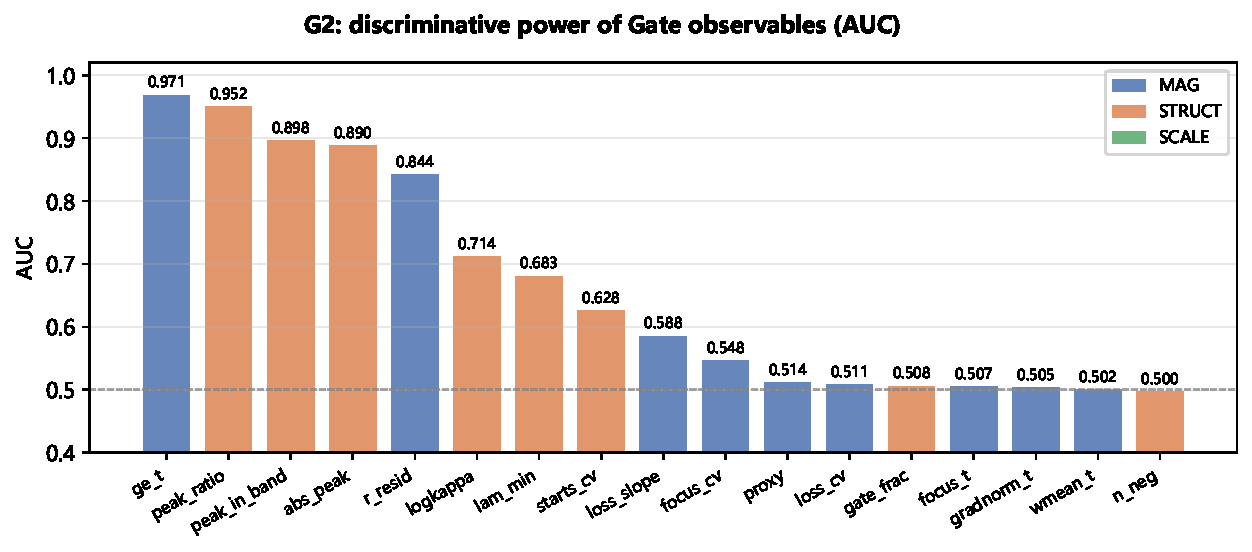
\includegraphics[width=0.92\textwidth]{fig_G2_auc_en.pdf}
\caption{Experiment 6.1: discrimination ability (AUC, $n=80$, proxy-label convention) of the Gate observables. The gradient-energy--contrast $g_{et}$ (MAG group) has the highest AUC (.971); within the structural group (STRUCT), peak ratio $.95$, in-band mass $.90$, and absolute peak $.89$ are strong, with the remaining group members at $.50$--$.71$; the independent-grid residual RMS $r_{\rm resid}$ (MAG group) is $.84$ in the proxy convention but only $.51$ in the oracle-existence convention (acceptance/existence split, see the three-layer reading in the text); training-process quantities ($7$) have median AUC $.51$ (near chance level, non-discriminative), consistent with the identifiability analysis of \S\ref{sec:gate}.}\label{fig:g2auc}
\end{figure}

\FloatBarrier

\section{Cross-Equation Verification}\label{sec:crosseqn}

Under the same two-phase protocol as for Burgers, this section examines the applicability of this paper's conclusions to other equation types. The core question is: \emph{do the capability boundaries of spatial weighting depend on the specific structure of Burgers?} The conclusions are: on the smooth elliptic Poisson equation, up-weighting has no systematic benefit (degeneracy verification); on internal-singularity problems, representation-level defects dominate and spatial weighting is powerless (a falsifiable prediction of level separation); and two lightweight examples---1D time-dependent Burgers (Experiment 7.5) and 2D linear convection--diffusion (Experiment 7.7)---test the directional stability of the above boundaries under time dependence and higher dimension.

\subsection{Poisson Smooth-Degeneracy Control (Experiment 7.1, $n=11$)}\label{sec:s2a}

\textbf{Setup.} An elliptic Poisson equation calibrated by an analytic solution, with two solution types: single-frequency and multi-frequency containing a $3\pi$ high frequency; representers: a plain MLP, matched-bandwidth Fourier features ($\sigma=1$), and mismatched high bandwidth ($\sigma=15$); weights: uniform, rational up-weighting, and inverse down-weighting, $7$ weight--contrast combinations in total; $n=11$ seeds per cell, fixed $3000$ steps, $462$ trainings in total. The Poisson solution is smooth, shock-free, used to test ``whether spatial weighting still pays off without local stiffness''; the paired test is Wilcoxon signed-rank.

\noindent\textbf{Three conclusions (paired, $n=11$)}.
(i)~\emph{Up-weighting has no systematic benefit on smooth problems}: of six up-weighting ($\beta=10$)-vs-uniform paired Wilcoxon contrasts, five are insignificant; the only significant group is (single-frequency, $\sigma=1$): the median $L_2$ in fact rises from $1.41\times10^{-5}$ to $1.11\times10^{-4}$ ($p=.001$; per-seed paired worsening factor median about $5$; in this subsection all factors are medians of per-seed paired factors, and group medians only describe group levels). This is consistent with Mechanism A's prediction (the contrast-separability condition fails at the smooth end; up-weighting brings no benefit), but terminal-state comparison cannot precisely distinguish the two mechanistic attributions ``gradient-scale modulation'' vs ``implicit spectral alignment''; this is only a directional-consistency observation.
(ii)~\emph{The significant benefit of inverse down-weighting appears mainly when ``the solution contains high frequencies while the representation bandwidth is insufficient/spectrally mismatched''}: multi-frequency solution with a plain MLP: median $L_2$ drops from $7.42\times10^{-3}$ to $2.02\times10^{-4}$ ($p=.001$, $11/11$ all improved, paired improvement-factor median about $24$); single-frequency, $\sigma=1$: from $1.41\times10^{-5}$ to $4.05\times10^{-6}$ ($p=.005$, $9/11$ improved, paired-factor median about $3.3$; here the absolute error is already at the $10^{-5}$ level, close to the error floor, so the practical significance of this gain is limited); mismatched high bandwidth (multi-frequency, $\sigma=15$): rises from $.108$ to $.113$ ($p=.001$, significantly worse). This corroborates Experiment 4.3: down-weighting is a gradient-scale modulator whose benefit does not require local stiffness but rather gradient-scale imbalance caused by spectral mismatch.
(iii)~\emph{Bandwidth--scale matching dominates}: mismatched high bandwidth is $40$--$1000\times$ worse than matched bandwidth on smooth solutions, irrecoverable by any of the three weightings; matching the representer bandwidth to the solution scale precedes and outweighs spatial weighting.

\subsection{Internal-Singularity Closed Loop (Experiments 7.4/7.2/7.3)}\label{sec:s2singular}

\paragraph{Unified framework: forward ansatz, wedge error, and three classes of representation-level interventions.} The forward representation is uniformly written as
\[
u(x)=A(X(x))+B(X(x))\,N(\gamma(X(x))),
\]
where $A$ is the boundary lifting, $B$ the annihilating factor satisfying homogeneous boundary conditions, $X$ the coordinate mapping, and $\gamma$ the input features/frequencies. For the commonly used $B(x)=1-x^2$ on $(-1,1)$, the network part's deviation from the lifting has the pointwise wedge bound
\begin{equation}\label{eq:wedge}
|u(x)-A(x)|\le (1-x^2)\,\|N\|_\infty .
\end{equation}
The wedge width is $O(1)$ in the domain interior (the network has ample corrective power) and degenerates to $0$ at the boundary $x\to\pm1$ (no corrective power; the boundary-layer shape must be built exactly into $A$). Accordingly, representation-level interventions are divided into three classes: \textbf{Type-I (boundary encoding)} (modifying $A/B$), \textbf{Type-II (coordinates and measure)} (modifying $X$), \textbf{Type-III (internal topological defects)} (modulating $\gamma$ and initial values by the position/topology of internal defects). Spatial weighting and multi-start do \emph{not} change $A,B,X,\gamma$, hence are powerless against the capability defects of Types-I/II/III; this is the falsifiable prediction of level separation in the cross-equation case.

\paragraph{Experiment 7.2 internal turning-point layer (positive geometric transfer of Type-II, full $n=11$).} The equation $-\varepsilon u''-xu'=0$, $u(-1)=0,u(1)=1$, has an error-function true solution with the layer at the interior $x=0$. $\varepsilon=.01/.001/10^{-4}$ (equivalent Burgers viscosities $\nu_{\rm eq}=.058/.018/.0058$, calibrated by empirically pairing the internal error-function layer with a Burgers shock layer of equal thickness---an empirical pairing, not an analytic equivalence). Under the same two-phase protocol as Burgers, \textbf{[empirical $n=11$]}: at all three thicknesses, $K=4$ selection gives $11/11$ entry into refinable basins, and after refinement the global relative $L_2$ median is of order $10^{-5}$. The internal defect sits at the widest part of the wedge and is refined without any boundary lifting or topological seeding.

\noindent\textbf{Conditionality of Mechanism A on this example (contrasted with Burgers).} Freezing the Gate point, same $\theta$ same $r$, only changing $\beta\in\{1,3,8\}$: the zonal gradient-energy ratio $\eta=g_{\rm band}/g_{\rm smooth}$ decreases at $7/11$ Gate points and increases at $4/11$, with mean Spearman rank correlation about $-0.32$ (\textbf{in contrast to Burgers, where all four viscosities give $+1$}); the reason is that $\beta$ amplifies both layer-band and smooth-region gradients, while at this linear layer's Gate point the layer is already essentially formed and in-band contrast separation (C-Sep) is weak. Paired refinement (layer-region $L_2$): $\beta=3$ vs $\beta=1$ is better in $8/11$, median difference $-1.06\times10^{-5}$ (Wilcoxon two-sided $p=.41$, Holm-corrected $p=.56$); $\beta=8$ is $7/11$ ($p=.28$, corrected $p=.56$)---\emph{both insignificant}; after refinement at all three levels, $L_2$ falls in $10^{-5}$--$10^{-4}$, converging to the accuracy floor determined by the Fourier bandwidth. This is not a negative result but pins down the applicability boundary of Mechanism A: the energy-redistribution benefit of up-weighting strictly depends on in-band contrast separation (C-Sep) at the Gate point and on local stiffness; when the problem is linear, the layer center sits at the widest wedge, there are no bad basins, and the accuracy bottleneck is the representation bandwidth, $\beta$ is neutral---together with the Poisson smooth degeneracy (Experiment 7.1)'s ``up-weighting has no systematic benefit,'' the two sides squeeze out the same boundary.

\paragraph{Experiment 7.3 Allen--Cahn spike (Type-III: expressible $\ne$ reachable, diagnostic level).} The equation $-\varepsilon^2u''+u-u^3=0$ admits a homoclinic spike $u^*(x)=\sqrt2\,\mathrm{sech}((x-x_0)/\varepsilon)$ and the zero-energy ground state $u\equiv0$. Taking $\varepsilon\in\{.01,.0044,.002\}$, a plain $K=4$ network, $4$ starts per level: \emph{without seeding}, $12/12$ all collapse to $u\equiv0$ (the residual can be driven to near zero---$u\equiv0$ is itself a zero-residual solution---while the global $L_2\approx.999$), even though $u^*$ is $\varepsilon_0$-expressible in this network class to accuracy far above what beating the zero-collapse rate requires (a purely supervised fitting control with fixed target $u^*$, $12$ independent seeds: global normalized $L_2$ median $6.2\times10^{-4}$, about three orders of magnitude below the collapsed state's $.999$)---this is a controlled counterexample of ``expressible $\ne$ reachable'': the defect lies not in representation capacity but in optimization reachability (the topology of the $\theta$ initialization). Switching to topological seeding centered at $x_0$ ($\varepsilon=.0044$, $4$ starts per method): exact sech seeds hit $4/4$; coarse Gaussian seeds at amplitude $.8/\sqrt2/2$ and width $1.5\varepsilon$ all hit $4/4$; only when the seed is misplaced at $x_0=.15$ ($\approx34\varepsilon$) do $4/4$ fail, the peak annihilated. That is, topological seeds \emph{must be right in position but can be coarse in shape/amplitude/width}; they modulate the $\theta$ initialization with zeroth-order representation information, acting at the representation--optimization interface.

\paragraph{Experiment 7.4 boundary-hugging convection--diffusion layer (Type-I: boundary not correctable, diagnostic level).} The equation $-\varepsilon u''+bu'=0$ has its layer at the boundary $x=1$, an exponential true solution, no shock. Paired by layer thickness to the equivalent $\nu=.005$ ($\varepsilon=.01$): at the same thickness, Burgers with $K=8$ gets $3$ hits out of $8$ starts, while the boundary-hugging layer gets $16/16$ zero hits at $\sigma=15/30$ ($L_2=9.6$--$10.8$). Changing only the coordinate map $X$ (Type-II): the thick layer $\varepsilon=.1$ stretches to $4/4$ success, the thin layer $\varepsilon=.01$ stretches to $8/8$ failure---stretching only rearranges the measure; it does not supply the corrective power missing at the boundary-hugging wedge. Changing the boundary lifting $A$ (Type-I): the exact exponential lifting succeeds $4/4$ (global $1.6\times10^{-3}$--$3.3\times10^{-3}$), the coarse logistic lifting fails $8/8$. The boundary-hugging layer's wedge degenerates to zero, so the layer shape \emph{must} be built exactly into $A$---a perfect contrast to internal defects' ``coarse geometry suffices.''

\begin{figure}[ht]\centering
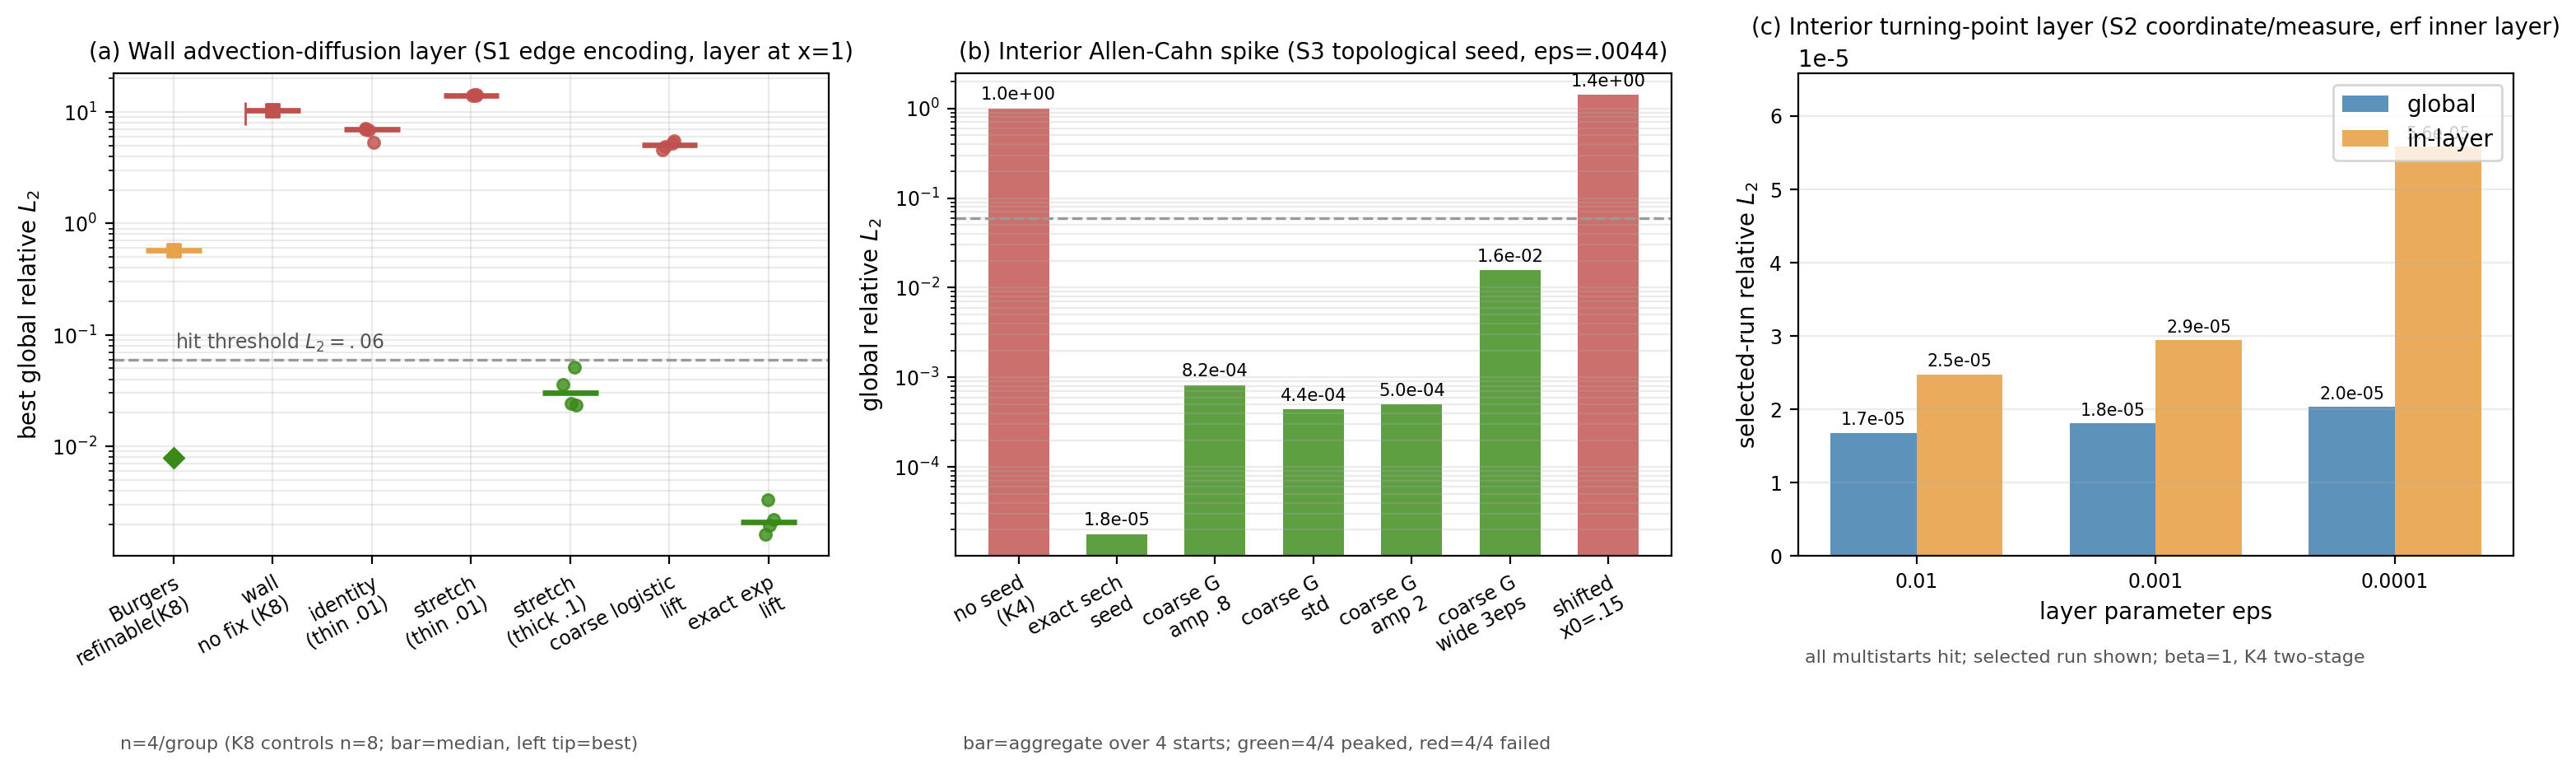
\includegraphics[width=0.99\linewidth]{fig_s2_singular_panel_en.png}
\caption{(Quantitative; Experiment 7.2 full $n=11$, Experiments 7.4/7.3 diagnostic level) (a) Boundary-hugging convection--diffusion layer: only the exact exponential lifting (Type-I) and the thick-layer coordinate stretching (Type-II) succeed; thin-layer stretching, coarse lifting, and no intervention all fail; (b) Allen--Cahn internal spike: without seeding $12/12$ collapse to zero; centered topological seeds form the spike $4/4$; misplacement by $34\varepsilon$ fails $4/4$; (c) the internal turning-point layer at all three thicknesses refines to the $10^{-5}$ scale.}\label{fig:s2panel}
\end{figure}

\subsection{One-Dimensional Time-Dependent Burgers (Experiment 7.5, $n=11$)}\label{sec:d1}

\textbf{Setup.} Time-dependent viscous Burgers $u_t+uu_x=\nu u_{xx}$, $x\in[-1,1]$, $t\in[0,.99]$, $\nu=.01/\pi$, initial condition $u(x,0)=-\sin(\pi x)$, boundary conditions $u(\pm1,t)=0$ (the Raissi standard example, soft boundary), reference solution taken as a high-resolution spectral/numerical solution. Network $[2,50,50,50,50,1]$ ($p=7851$), collocation $N=4300$ ($4000$ PDE $+100$ BC $+200$ IC), fixed-step Adam for $50000$ steps, weights from the rational up-weighting family $w=(1+\beta t)/(1+t)$ ($t=|r|/\mathrm{median}|r|$, same family as the steady-state Experiments 5.4/5.5), strengths $\beta\in\{1,3,8,15\}$, $n=11$ equally spaced seeds per cell (the same base seed set $S_0=\{0,5,\dots,50\}$ as the steady-state experiments). The good-basin threshold $\tau=.06$ is calibrated by the natural gap in the space-time-domain relative $L_2$ (the sorted values of all four levels leave a gap near $.056$--$.066$; see the table note for the threshold scan).

\begin{table}[ht]\centering\small\renewcommand{\arraystretch}{1.2}
\begin{tabular}{cccc}
\toprule
$\beta$ & Median space-time $L_2$ & $L_2$ range & Good basins/$11$\\
\midrule
$1$  & $1.66\times10^{-2}$ & $[2.87\times10^{-3},\,.327]$ & $8$\\
$3$  & $1.53\times10^{-2}$ & $[6.56\times10^{-3},\,.150]$ & $9$\\
$8$  & $5.56\times10^{-2}$ & $[1.80\times10^{-2},\,.375]$ & $6$\\
$15$ & $5.35\times10^{-2}$ & $[2.90\times10^{-2},\,.105]$ & $8$\\
\bottomrule
\end{tabular}
\caption{(Quantitative, Experiment 7.5, $n=11$) Space-time-domain relative $L_2$ median, range, and good-basin count (threshold $\tau=.06$, lying inside the natural gap of the sorted values of all four levels) for different fixed strengths on 1D time-dependent Burgers. The good-basin counts of the $\beta=8/15$ levels are threshold-sensitive: at $\tau=.05/.06/.10$, $\beta=8$ gives $4/6/8$ and $\beta=15$ gives $5/8/10$; the per-seed paired tests do not depend on the threshold value.}\label{tab:d1beta}
\end{table}

\noindent\textbf{Conclusions (Table~\ref{tab:d1beta}).}\textbf{[empirical $n=11$]}(i)~The good/bad basin distinction persists on time-dependent problems (all four levels have failing seeds; the good-basin counts for $\beta=1/3/8/15$ are $8/9/6/8$, with failures showing a long tail up to $.1$--$.4$), but the stable, symmetric pseudo-solution bimodality of the 1D steady stiff end is not observed; the basin structure is sensitive to time stepping and boundary treatment. (ii)~Paired Wilcoxon signed-rank tests show no significant differences between levels ($\beta=1$ vs $3/8/15$: $p=.41/.32/.37$, $n_{\rm eff}=11$); the per-seed best is taken by $\beta=3$ in $6/11$ cases, by $\beta=1$ in $4/11$, and by $\beta=15$ in $1/11$; high-strength up-weighting both rescues catastrophic failures of $\beta=1$ (e.g., seed 30 drops from $.327$ to $.029$) and creates failures on new seeds (the median $L_2$ ratio of $\beta=8$ to $\beta=1$ is $3.95$, worst nearly $100\times$), with wins and losses canceling out. That is, rational up-weighting on time-dependent Burgers is \emph{near-neutral}: Mechanism~A fires as usual ((iii)) but converts into neither systematic gains nor systematic failures. On the same equation the spatial linear family yields ``up-weighting is harmful'' (zero good basins at $\beta=8/15$), while an earlier scan with the spatial linear family under a different $\nu$/seed convention claimed ``up-weighting is beneficial''---the reversal of the conclusion across weight families itself shows that the time-dependent basin structure is sensitive to the weight family and protocol. Together with Experiments 7.1/7.2/7.7, this section confirms: spatial weighting brings no systematic gains on time-dependent and smooth/linear problems. (iii)~\emph{Mechanism-A cross-equation corroboration}: freezing at the Gate point, same $\theta$ same $r$, only switching $\beta=1$ to $8$: the cosine between the weighted and unweighted gradient directions has median $.9999$ (range $.999$--$1.000$, direction nearly unchanged), the total gradient-norm ratio has median $7.75$ ($7.15$--$7.84$, $\approx\beta$, a global scale amplification), and the ratio of central-region to boundary-region gradient row norms rises from $2.90$ to $4.20$; that is, up-weighting mainly performs a spatial redistribution of gradient scale while barely changing the gradient direction---consistent with the steady-state characterization of Mechanism~A.

\par\smallskip\noindent\textbf{Diagnostic-level observation (artificial bad basin, Experiment 7.6, $n=11$, Adam $20000$ steps).} After artificially placing the initialization in a bad basin (terminal $L_2\approx2.5$, $0/11$ enter good basins) via means such as zero initial values: down-weighting $\beta=1/3,\,1/8$ (spatial linear family) gives median $L_2=2.75/2.86$ (\emph{worse}), gradient clipping (thresholds $.01/.1$) is bitwise identical to the control ($2.57$, terminal state unchanged), and mild up-weighting $\beta=3,\,8$ ($2.44$) still stays in the bad basin. That is, once the initialization falls into a bad basin, neither spatial down-weighting nor explicit gradient clipping can rescue it---mutually corroborating the steady-state Experiment 5.3 conclusion that ``down-weighting is not a basin-escape mechanism,'' and clipping is likewise ineffective in the time-dependent case. This setup is an artificially constructed diagnostic experiment, not the natural training distribution; systematic time-dependent paired experiments are left to future work.

\begin{figure}[ht]\centering
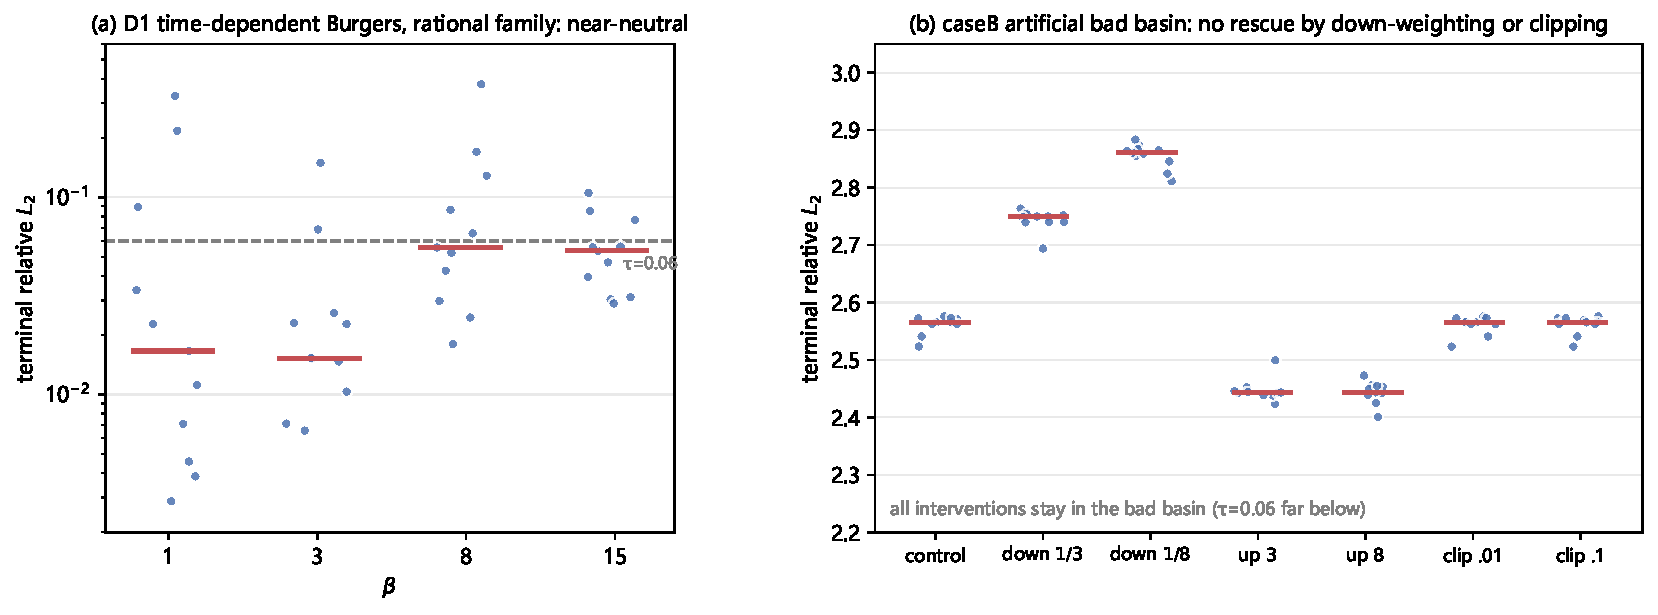
\includegraphics[width=0.98\textwidth]{fig_d1_caseb_en.pdf}
\caption{(a)~Experiment 7.5 (1D time-dependent Burgers, rational family, $n=11$): per-seed space-time-domain relative $L_2$ at four fixed strengths (log scale); the dashed line marks the good-basin threshold $\tau=.06$. Every level has failing seeds and paired tests show no significant differences ($p=.41/.32/.37$): rational up-weighting is near-neutral. (b)~Experiment 7.6 artificial bad-basin diagnosis (spatial linear family, $n=11$, Adam $20000$ steps, diagnostic level): terminal $L_2$ distributions under down-weighting $\beta=1/3,\,1/8$, gradient clipping (thresholds $.01/.1$), and mild up-weighting $\beta=3,\,8$ versus control; no intervention escapes the bad basin (clipping is bitwise identical to control).}\label{fig:d1caseb}
\end{figure}

\subsection{Two-Dimensional Linear Convection--Diffusion (Experiment 7.7, $n=11$)}\label{sec:c45}

\textbf{Setup.} The 2D linear convection--diffusion equation (periodic boundary conditions, with an initial condition); the solution is smooth, without internal shocks or thin boundary layers; network input dimension $d_{\rm in}=3+4K$ ($K=32$ Fourier features), $p=14301$, collocation $N=4200$ ($4000$ PDE $+200$ IC), fixed-step Adam. A uniform-weight ($\beta=1$) baseline is run first, followed by a scan over $\beta\in\{1,3,8\}$, with $n=11$ equally spaced seeds per cell.

\begin{table}[ht]\centering\small\renewcommand{\arraystretch}{1.2}
\begin{tabular}{cccc}
\toprule
$\beta$ & Median $L_2$ & $L_2$ range & Max $L_2$\\
\midrule
$1$ & $5.06\times10^{-2}$ & $[.0461,\,.0628]$ & $.0628$\\
$3$ & $5.03\times10^{-2}$ & $[.0418,\,.0582]$ & $.0582$\\
$8$ & $4.85\times10^{-2}$ & $[.0414,\,.0583]$ & $.0583$\\
\bottomrule
\end{tabular}
\caption{(Quantitative, Experiment 7.7, $n=11$) Space-time-domain relative $L_2$ median, range, and maximum for different fixed strengths on 2D linear convection--diffusion; all $33$ runs have $L_2\le.0628$ with no failing seeds, so no good-basin threshold is set for this example.}\label{tab:c45}
\end{table}

\noindent\textbf{Conclusions (Table~\ref{tab:c45}, single configuration, direction-level illustration).}\textbf{[empirical $n=11$]} All $33$ runs have $L_2\le.0628$ with no failing seeds; no pseudo-solution bimodality is observed; from $\beta=1\to8$ the median $L_2$ only goes $.0506\to.0485$ (a same-order fluctuation of about $4\%$)---spatial weighting is nearly neutral. Together with the Poisson smooth degeneracy (Experiment 7.1), from the 1D and 2D sides they jointly confirm: on smooth/linear problems with neither local stiffness contrast (C-Sep fails) nor bad basins, spatial weighting brings no systematic benefit and manufactures no failure.

\begin{figure}[ht]\centering
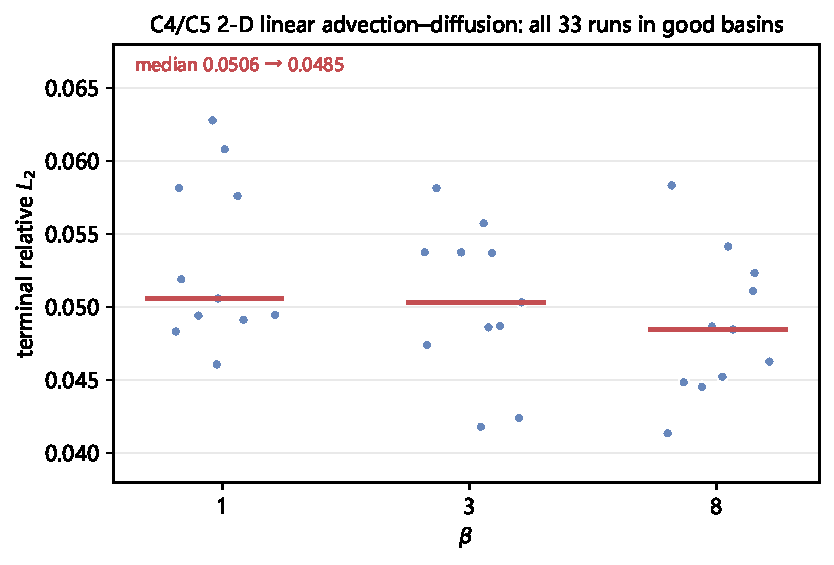
\includegraphics[width=0.85\textwidth]{fig_c45_advdiff_en.pdf}
\caption{(Quantitative, Experiment 7.7, $n=11$) Per-seed space-time-domain relative $L_2$ of all $33$ runs at $\beta=1/3/8$ on 2D linear convection--diffusion (dashed line $\tau=.06$ is the Experiment 7.5 good-basin threshold, shown for reference only): all $33$ runs have $L_2\le.0628$ with no failing seeds, the three levels overlap heavily, and spatial weighting is nearly neutral.}\label{fig:c45}
\end{figure}

\noindent\textbf{Summary of cross-equation verification.} The above prototypes (Figure~\ref{fig:s2panel}) close the loop, in the steady 1D case, on the discriminative power of the ``three-class representation-level taxonomy'': internal defects (Experiment 7.2) sit at the widest wedge and spatial weighting is neutral; internal topological defects (Experiment 7.3) require topological seeding and spatial weighting is powerless; boundary-hugging layers (Experiment 7.4) require exact boundary lifting and spatial weighting is powerless. Together the three verify the falsifiable prediction of level separation: spatial weighting does not change the representation-level $A,B,X,\gamma$, hence is powerless against representation-level defects. Beyond this, on 1D time-dependent Burgers (Experiment 7.5, \S\ref{sec:d1}), high-strength fixed up-weighting likewise brings no systematic benefit, and neither down-weighting nor clipping can rescue artificial bad basins, while Mechanism~A's ``up-weighting amplifies scale and barely changes direction'' reproduces in the time-dependent case; on 2D linear convection--diffusion (Experiment 7.7, \S\ref{sec:c45}) all $33$ runs finish without failure ($L_2\le.0628$) and weighting is nearly neutral. Hyperbolic/system cases such as water hammer and shallow water, and 2D stiff examples, are left to future work under the same controlled protocol.

\FloatBarrier

\section{Scope and Conclusions}\label{sec:conclusion}

\subsection{Equation-Independent Core and Equation-Dependent Constants}\label{sec:scope}

The certain conclusions of this paper fall into two layers. The \emph{equation-independent core} (under each proposition's own assumptions, independent of Burgers structure and applicable to general smooth PDEs and network architectures) includes: invariance of the zero-residual set under positive weights (Proposition~\ref{prop:zero}); the linear part of the residual--error bridge (Proposition~\ref{prop:bridge}); the spectral capability boundary of local diagonal weights (Theorem~\ref{thm:local-cap}, using only simultaneous diagonalization, the correlation-matrix identity, and the van der Sluis theorem); condition-number optimality of the equicorrelation class under diagonal scaling (Theorem~\ref{thm:equicorr}); the identifiability lower bound of fixed single-projection scalars and the four-point counterexample (Proposition~\ref{prop:bayes}); and the first-order directional criterion for up-/down-weighting (Proposition~\ref{prop:align}). The \emph{statements} of these conclusions do not depend on the specific equation, but the \emph{constants} involved (e.g., the stability constant $C_{\rm loc}$, the condition number $\kappa(K_r)$, the effective rank $PR$, the degree of contrast separation C-Sep) are equation- and parameter-dependent.

The \emph{equation-dependent empirical conclusions} (verified on 1D steady Burgers, to be re-examined on other equations) include: the $\eta_{gate}$ monotonicity of Mechanism A (Experiments 5.1/5.2); the non-observation that down-weighting improves the basin-entry probability (Experiment 5.3, $n=80$); the regime of $\beta^*$ inside refinable basins (Experiments 5.4/5.5/5.6, $n=11$); dynamic records of the in-training Hessian condition number (Experiment 4.3); the feasibility of the structural quantity $g_et$ in ground-truth-free discrimination (Experiment 6.1, $n=80$). The \emph{qualitative directions} of these conclusions (no observation that spatial weighting can select basins; up-weighting gains depend on local stiffness; down-weighting is a gradient-scale modulator whose benefit depends on whether scale is the bottleneck) have been cross-equation-verified on Poisson (Experiment 7.1) and internal singularities (Experiments 7.4/7.2/7.3), but the \emph{quantitative constants} (e.g., the specific value of $\beta^*$, the gain factors) are equation-dependent.

\subsection{Criteria for Migration to New Weight Families and New Equations}\label{sec:migration}

The applicability conditions for migrating this paper's conclusions to new weight families are as follows:
\begin{enumerate}[label=(\arabic*),leftmargin=2em,itemsep=1pt]
\item \textbf{Positive diagonal, pointwise (local) multiplicative weights}: when this holds, the spectral capability boundary of Theorem~\ref{thm:local-cap} applies directly; introducing non-diagonal (convolution/operator preconditioning) or trainable weights $\W(\theta)$ exceeds the framework of this paper.
\item \textbf{Principles I--II (the gradient-only class)}: when the weights are triggered by quantities containing $\W$ (e.g., adaptively adjusted by the weighted loss $L_\W$), Principle~II is violated and the case is not covered here.
\item \textbf{Weights frozen or exogenously slowly varying}: when $w(t_i(\theta))$ is recomputed every step, $\nabla_\theta\W\ne0$, the weighted gradient is no longer $J^\top\W r$, and the linearization framework of this paper does not apply directly.
\end{enumerate}

When migrating to new equations, the following properties determine whether this paper's qualitative conclusions are expected to persist:
\begin{enumerate}[label=(\arabic*),leftmargin=2em,itemsep=1pt]
\item \textbf{Local stiffness contrast (C-Sep)}: when absent (e.g., smooth Poisson), the up-weighting benefit of Mechanism A is expected to vanish.
\item \textbf{Bistable good/pseudo-solution basin structure}: when absent (e.g., the internal turning-point layer Experiment 7.2), the basin-selection problem does not arise and the operating window of spatial weighting shrinks.
\item \textbf{Representer--scale matching}: when the representation bandwidth mismatches the solution scale (e.g., fixed high bandwidth at the smooth end), representation-level defects dominate and spatial weighting cannot recover.
\end{enumerate}

\subsection{Relation Between Jacobi Equilibration and Gradient-Norm Weighting}\label{sec:jacobi-gap}

The Experiment 4.2 triplet shows that of the gap between the practitioner's starting point (uniform weight $\kappa(K_r)$) and the unconstrained ceiling ($\kappa^*_{\rm diag}$), $>85\%$ in the linear-gap convention can be filled by the simple local diagonal weight of Jacobi equilibration $w_i\propto(K_r)_{ii}^{-1/2}$. This paper's spectral scan covers the rational family (Table~\ref{tab:f1d-triplet}): its in-family optimum is always $\beta=1$ (uniform weight), an order-of-magnitude gap from Jacobi; the other contrast families were not spectrally scanned, and this paper makes no claim about their spectral properties.

In the PINN context, Jacobi equilibration is exactly \emph{gradient-norm weighting}: $(K_r)_{ii}=\|J_i\|^2$ is the squared row norm of the residual gradient at collocation point $i$, so $w_i\propto 1/\|J_i\|$. This belongs to the same family of methods as the learning-rate annealing proposed by Wang, Teng, and Perdikaris \cite{WangTeng2020} (adjusting each loss term's learning rate by gradient-norm ratios)---Experiment 4.2 provides a \emph{second-order spectral mechanistic explanation} for the effectiveness of annealing: gradient-norm normalization is exactly Jacobi equilibration, which can pull the condition number from the uniform-weight level down to the level of the correlation matrix $R(K_r)$, a step that the rational family cannot even reach (its in-family optimum is the uniform weight, see above).

This paper has \emph{not} tested dynamic Jacobi weighting in training experiments (recomputing $w_i\propto 1/\|J_i(\theta)\|$ every step), for two reasons: (1) dynamic Jacobi is online recomputation $\W(\theta)$, violating Principle~II ($\nabla_\theta\W\ne0$), beyond the theoretical coverage of this paper's frozen/exogenous-slow-variation convention; (2) the per-step row-norm computation costs $O(Np)$, unlike the $O(N)$ of contrast weights. Static Jacobi (frozen once at the Gate point) falls within the exogenous-slow-variation convention, is theoretically covered, and is a low-cost future direction; the corrected-gradient analysis of dynamic Jacobi ($g=J^\top\diag(m_{ad})r$, see Lemma~\ref{lem:linrec}(ii)) and the channel-$\theta$ effect of online weighting are listed as future work (\S\ref{sec:future}).

\subsection{Empirical Observation: The Second-Order Spectrum Does Not Determine Basins; the Representation Level Dominates}\label{sec:S-observation}

All experiments of this paper consistently point to one observation beyond the ``capability boundary of weighting'': with the network representation fixed (architecture, boundary encoding, coordinate mapping, Fourier feature bandwidth), spatial weighting does not change the attraction-basin topology of the loss landscape, only the scale distribution of gradients; the existence and reachability of basins are determined by the representation level's expressive power and encoding geometry. Supporting evidence:

\begin{enumerate}[label=(\arabic*),leftmargin=2em,itemsep=1pt]
\item \textbf{Boundary encoding (Type-I) changes basins}: the hard-boundary ansatz ($u=(1-x^2)v$) and the soft boundary (loss-term penalty) are two different zeroth-order representations; errors in hard-boundary amplitude encoding pin the endpoint error (see the reproduction-details B.5 audit), while the time-dependent example Experiment 7.5 trains under the soft-boundary setting. We observe a qualitative difference in training behavior between the two encodings at the high-viscosity end, but we have \emph{not} made a strict soft/hard paired control at the same configuration, so this is only directional evidence; systematic comparison is left to future work.
\item \textbf{Coordinates and measure (Type-II) and the geometric conflict with boundary layers}: in the elliptic boundary-layer example Experiment 7.4, the hard-boundary encoding conflicts with the geometric structure of the boundary layer, which can only be relieved by relying on the true-solution structure (coordinate stretching); pure spatial weighting cannot solve it. The internal-singularity examples Experiment 7.2/Experiment 7.3 show that $u\equiv0$ is a stable local minimum and initialization sensitivity dominates---``representable $\neq$ reachable.''
\item \textbf{Matching of representation bandwidth and solution scale (Type-III, feature/topology side)}: when the Fourier feature bandwidth $\sigma$ mismatches the solution scale (fixed high bandwidth at the smooth end), representation-level defects dominate and spatial weighting cannot recover (Experiment 5.6 degeneracy scan); the root cause of high-viscosity degeneracy is insufficient bandwidth, not improper weights.
\item \textbf{Second-order interventions do not raise, and down-weighting families lower, basin entry}: Experiment 5.3 ($n=80$) shows no weight family raises the entry rate, with uniform's hit rate $.613$ the highest; the down-weighting family down\_lin \emph{significantly lowers} the entry rate after Holm correction ($.388$, corrected $p=.006$), and down\_inv/rational are also below uniform. That is, spatial weighting (at least the down-weighting families) is measured to change basin-membership probabilities, in the negative direction; Experiment 5.9 shows no significant terminal-state difference among the four families under fixed-step L-BFGS.
\end{enumerate}

A corollary of this observation is: for the many claims in the literature that ``weighting improves training,'' the benefit may actually come from the accompanying representation-level changes (e.g., adaptive sampling changes the measure; hard-boundary encoding changes the representation) rather than from the weights themselves. Strictly separating interventions at the zeroth/first/second order is a necessary premise for understanding PINN training mechanisms. This observation is an empirical induction (\textbf{[empirical]}), not a rigorous theorem; its formalization and systematic classification are listed as future work (\S\ref{sec:future}, item 3).

\subsection{Future Work and Open Problems}\label{sec:future}

This paper has delineated the capability boundary of spatial static weighting under the above stratification. The following directions exceed this paper's scope and are listed as future work:

\begin{enumerate}[label=(\arabic*),leftmargin=2em,itemsep=1pt]
\item \textbf{A constructive training theory for channel $\theta$}: alignment of the in-basin first-order directional criterion with the two reference frames ``own-basin stationary point / true solution''; conditional existence of the in-basin optimal strength $\beta^*$ and a multi-term decomposition of the error; safe switching conditions from down- to up-weighting; two-phase conditional error bounds incorporating the entry probability $p_{entry}(1-\delta)$.
\item \textbf{Multi-level synergy and conflict}: designing new algorithms under the above stratification; studying whether interventions at the zeroth order (representation), second order (spectrum), and first order (optimization dynamics) reinforce or fight each other; rigorous analysis of non-local/convolutional weights, operator preconditioning, and online adaptive weights.
\item \textbf{Classification properties of the representation level}: based on this paper's Experiments 7.4/7.2/7.3 findings, systematically study the capability boundaries and a unified framework of the three classes of representation-level interventions---boundary encoding, coordinates and measure, internal topological defects; the effect of hard-boundary treatments on the representation level.
\item \textbf{Cross-equation and time-dependent/high-dimensional verification}: this paper has done lightweight cross-equation verification on 1D time-dependent Burgers (Experiment 7.5) and 2D linear convection--diffusion (Experiment 7.7); hyperbolic/system cases such as water hammer and shallow water, 2D stiff Burgers and systematic time-dependent paired experiments remain to be done. Reference solutions are preferably open-source (BSD/MIT licensed) high-resolution ones.
\item \textbf{Deepening the Gate methodology}: calibrating the efficacy of Gate-A's three trigger rules (when all three hold, with what probability is one in a refinable basin; can some rule be removed; weakest testable substitutes); the minimal sufficient set of structural quantities and its compactness; sufficient conditions for cross-viscosity, cross-equation deployment.
\end{enumerate}

\noindent\textbf{Summary.} This paper rigorously characterizes the capability boundary of spatial static diagonal weighting at the zeroth/first/second orders: at the second-order level, local diagonal weights cannot change the correlation matrix $R(K_r)$, do not improve the condition number on the equicorrelation class, and the optimal condition number is still unbounded when nearly singular (Theorem~\ref{thm:local-cap}, doubly verified by static Experiment 4.2 + dynamic Experiment 4.3); at the first-order level, we do not observe that weighting improves basin entry (Experiment 5.3, $n=80$ paired rejection of the down-weighting escape hypothesis, without universal negation), and its beneficial effects are confined to convergence-speed modulation inside already-entered refinable basins (up-weighting gains strictly depend on local stiffness contrast---Mechanism A, Experiments 5.4/5.5/5.6, $n=11$) and gradient-scale modulation (the true role of down-weighting, Experiment 4.3; terminal-state benefits under spectral mismatch in Section~\ref{sec:crosseqn}); methodologically, fixed single-projection scalars of the residual/loss self-evaluation type cannot reliably discriminate basin quality (Proposition~\ref{prop:bayes}, with Experiment 6.1 verifying the feasibility of the structural quantity $g_et$); in cross-equation verification, up-weighting has no systematic benefit on smooth Poisson (Experiment 7.1), and on internal-singularity problems representation-level defects dominate and spatial weighting is powerless (Experiments 7.4/7.2/7.3); on 1D time-dependent Burgers (Experiment 7.5) high-strength up-weighting has no systematic benefit and down-weighting/clipping cannot rescue artificial bad basins; on 2D linear convection--diffusion (Experiment 7.7) weighting is nearly neutral with no failing seeds ($L_2\le.0628$)---the capability boundary is directionally stable in time-dependent and higher-dimensional smooth/linear cases. This paper's contribution is the characterization of capability boundaries and controlled falsification, not the proposal of new algorithms; a constructive training theory and multi-channel cooperative algorithms are left to future work.

\FloatBarrier

\section*{Acknowledgments and Declaration of Generative AI Use}
During the preparation of this work the author used the AI assistants Doubao (ByteDance) and Kimi (Moonshot AI) in order to assist with literature cross-checking, language polishing, and code and data verification. After using these tools, the author reviewed and edited the content as needed and takes full responsibility for the content of the publication.

\section*{Data Availability}
All experiment code, processed data, and analysis scripts that reproduce the results of this paper are openly available at \url{https://github.com/wm2243/pinn-capability-boundary} (code under the MIT license, text and figures under CC-BY-4.0); raw run data are archived on Zenodo (DOI: ZENODO\_DOI).

\begin{thebibliography}{99}\small
\bibitem{Raissi2019} M.~Raissi, P.~Perdikaris, G.~E.~Karniadakis. Physics-informed neural networks: A deep learning framework for solving forward and inverse problems involving nonlinear partial differential equations. \emph{Journal of Computational Physics}, 378:686--707, 2019.
\bibitem{Karniadakis2021} G.~E.~Karniadakis, I.~G.~Kevrekidis, L.~Lu, P.~Perdikaris, S.~Wang, L.~Yang. Physics-informed machine learning. \emph{Nature Reviews Physics}, 3:422--440, 2021.
\bibitem{Cuomo2022} S.~Cuomo, V.~S.~Di~Cola, F.~Giampaolo, G.~Rozza, M.~Raissi, F.~Piccialli. Scientific machine learning through physics-informed neural networks: Where we are and what's next. \emph{Journal of Scientific Computing}, 92:88, 2022.
\bibitem{Shin2020} Y.~Shin, J.~Darbon, G.~E.~Karniadakis. On the convergence of physics informed neural networks for linear second-order elliptic and parabolic type PDEs. \emph{Communications in Computational Physics}, 28(5):2042--2074, 2020.
\bibitem{MishraMolinaro2020} S.~Mishra, R.~Molinaro. Estimates on the generalization error of physics-informed neural networks for approximating PDEs. arXiv:2006.16144, 2020.
\bibitem{DeRyckMishra2022} T.~De~Ryck, S.~Mishra. Error analysis for physics-informed neural networks approximating Kolmogorov PDEs. arXiv:2106.14473, 2021.
\bibitem{DeRyckMishra2024} T.~De~Ryck, S.~Mishra. Numerical analysis of physics-informed neural networks and related models in physics-informed machine learning. \emph{Acta Numerica}, 33:633--713, 2024.
\bibitem{vanDerMeer2020} R.~van~der~Meer, C.~Oosterlee, A.~Borovykh. Optimally weighted loss functions for solving PDEs with neural networks. \emph{Journal of Computational and Applied Mathematics}, 405:113887, 2022.
\bibitem{Maddu2021} S.~Maddu, D.~Sturm, C.~L.~M\"uller, I.~F.~Sbalzarini. Inverse-Dirichlet weighting enables reliable training of physics informed neural networks. \emph{Machine Learning: Science and Technology}, 3(1):015026, 2022; arXiv:2107.00940.
\bibitem{WangTeng2020} S.~Wang, Y.~Teng, P.~Perdikaris. Understanding and mitigating gradient flow pathologies in physics-informed neural networks. \emph{SIAM Journal on Scientific Computing}, 43(5):A3055--A3081, 2021.
\bibitem{Wang2020NTK} S.~Wang, X.~Yu, P.~Perdikaris. When and why PINNs fail to train: A neural tangent kernel perspective. \emph{Journal of Computational Physics}, 449:110768, 2022.
\bibitem{Jacot2018} A.~Jacot, F.~Gabriel, C.~Hongler. Neural tangent kernel: Convergence and generalization in neural networks. \emph{Advances in Neural Information Processing Systems (NeurIPS)}, 2018.
\bibitem{Liu2022down} L.~Liu, S.~Liu, H.~Xie, F.~Xiong, T.~Yu, M.~Xiao, L.~Liu, H.~Yong. Discontinuity computing using physics-informed neural networks. \emph{Journal of Scientific Computing}, 98:22, 2024.
\bibitem{LessEmphasis2022} Y.~Wang, C.~Xu, M.~Yang, J.~Zhang. Less emphasis on hard regions: Curriculum learning of physics-informed neural networks for singularly perturbed convection-diffusion-reaction problems. arXiv:2210.12685, 2022.
\bibitem{Wang2022causal} S.~Wang, S.~Sankaran, P.~Perdikaris. Respecting causality for training physics-informed neural networks. \emph{Computer Methods in Applied Mechanics and Engineering}, 421:116813, 2024.
\bibitem{ConFIG2025} Q.~Liu, M.~Chu, N.~Thuerey. ConFIG: Towards conflict-free training of physics-informed neural networks. \emph{International Conference on Learning Representations (ICLR)}, 2025.
\bibitem{Krishnapriyan2021} A.~Krishnapriyan, A.~Gholami, S.~Zhe, R.~Kirby, M.~W.~Mahoney. Characterizing possible failure modes in physics-informed neural networks. \emph{NeurIPS}, 2021.
\bibitem{Bengio2009} Y.~Bengio, J.~Louradour, R.~Collobert, J.~Weston. Curriculum learning. \emph{ICML}, 2009.
\bibitem{Hazan2016} E.~Hazan, K.~Levy, S.~Shalev-Shwartz. On graduated optimization for stochastic non-convex problems. \emph{ICML}, 2016.
\bibitem{Mobahi2015} H.~Mobahi, J.~W.~Fisher~III. A theoretical analysis of optimization by Gaussian continuation. \emph{AAAI}, 1205--1211, 2015.
\bibitem{Lee2016} J.~D.~Lee, M.~Simchowitz, M.~I.~Jordan, B.~Recht. Gradient descent only converges to minimizers. \emph{Conference on Learning Theory (COLT)}, 2016.
\bibitem{LiuZhuBelkin2021} C.~Liu, L.~Zhu, M.~Belkin. Loss landscapes and optimization in over-parameterized non-linear systems and neural networks. \emph{Applied and Computational Harmonic Analysis}, 59:85--116, 2022.
\bibitem{ZhouGeJin2021} M.~Zhou, R.~Ge, C.~Jin. A local convergence theory for mildly over-parameterized two-layer neural network. arXiv:2102.02410, 2021.
\bibitem{AttouchBolte} H.~Attouch, J.~Bolte, B.~F.~Svaiter. Convergence of descent methods for semi-algebraic and tame problems: Proximal algorithms, iterative methods and the {\L}ojasiewicz inequality. \emph{Mathematical Programming}, 137:91--124, 2013.
\bibitem{vanderSluis1969} A.~van~der~Sluis. Condition numbers and equilibration of matrices. \emph{Numerische Mathematik}, \textbf{14}(1):14--23, 1969.
\bibitem{Osborne1960} E.~E. Osborne. On pre-conditioning of matrices. \emph{Journal of the ACM}, 7(4):338--345, 1960.
\bibitem{RoosStynesTobiska1996} H.-G. Roos, M. Stynes, L. Tobiska. \emph{Numerical Methods for Singularly Perturbed Differential Equations: Convection--Diffusion and Flow Problems}. Springer, 1996.
\bibitem{Bhatia} R.~Bhatia. \emph{Matrix Analysis}. Springer, 1997.
\bibitem{HornJohnson} R.~A.~Horn, C.~R.~Johnson. \emph{Matrix Analysis} (2nd ed.). Cambridge University Press, 2013.
\bibitem{Strassen1965} V.~Strassen. The existence of probability measures with given marginals. \emph{Annals of Mathematical Statistics}, 36(2):423--439, 1965.
\bibitem{McClenny2020} L.~D.~McClenny, U.~M.~Braga-Neto. Self-adaptive physics-informed neural networks. \emph{Journal of Computational Physics}, 474:111722, 2023.
\bibitem{Nabian2021} M.~A.~Nabian, R.~J.~Gladstone, H.~Meidani. Efficient training of physics-informed neural networks via importance sampling. \emph{Computer-Aided Civil and Infrastructure Engineering}, 36(8):962--977, 2021.
\bibitem{Wu2022} C.~Wu, M.~Zhu, Q.~Tan, Y.~Kartha, L.~Lu. A comprehensive study of non-adaptive and residual-based adaptive sampling for physics-informed neural networks. \emph{Computer Methods in Applied Mechanics and Engineering}, 403:115671, 2023.
\bibitem{TangDAS2023} K.~Tang, X.~Wan, C.~Yang. DAS-PINNs: A deep adaptive sampling method for solving high-dimensional partial differential equations. \emph{Journal of Computational Physics}, 476:111868, 2023.
\bibitem{Rahaman2019} N.~Rahaman, A.~Baratin, D.~Arpit, et~al. On the spectral bias of neural networks. \emph{ICML}, 2019.
\bibitem{Tancik2020} M.~Tancik, P.~P.~Srinivasan, B.~Mildenhall, et~al. Fourier features let networks learn high frequency functions in low dimensional domains. \emph{NeurIPS}, 2020.
\bibitem{deRyckOp2024} T.~De~Ryck, F.~Bonnet, S.~Mishra, E.~de~B\'ezenac. An operator preconditioning perspective on training in physics-informed machine learning. \emph{International Conference on Learning Representations (ICLR)}, 2024; arXiv:2310.05801.
\bibitem{PCPINN2024} S.~Liu, C.~Su, J.~Yao, Z.~Hao, H.~Su, Y.~Wu, J.~Zhu. Preconditioning for physics-informed neural networks. \emph{Proceedings of the 41st International Conference on Machine Learning (ICML)}, 2024; arXiv:2402.00531.
\bibitem{SiYan2025} C.~Si, M.~Yan. Convolution-weighting method for the physics-informed neural network: A primal-dual optimization perspective. arXiv:2506.19805, 2025.
\bibitem{Rathore2024} P.~Rathore, W.~Lei, Z.~Frangella, L.~Lu, M.~Udell. Challenges in training PINNs: A loss landscape perspective. \emph{International Conference on Machine Learning (ICML)}, 2024; arXiv:2402.01868.
\bibitem{Bonfanti2024} A.~Bonfanti, G.~Bruno, C.~Cipriani. The challenges of the nonlinear regime for physics-informed neural networks. \emph{Advances in Neural Information Processing Systems (NeurIPS)}, 2024.
\bibitem{WangPseudo2026} S.~Wang, S.~Koohy, Y.~Lu, P.~Perdikaris. When PINNs go wrong: Pseudo-time stepping against spurious solutions. arXiv:2604.23528, 2026.
\bibitem{Rohrhofer2022} F.~M.~Rohrhofer, S.~Posch, C.~G\"o{\ss}nitzer, B.~C.~Geiger. On the role of fixed points of dynamical systems in training physics-informed neural networks. arXiv:2203.13648, 2022.
\bibitem{Musah2026} R.~Musah. Inverted model selection in physics-informed neural networks: when a lower residual selects a worse solution. arXiv:2608.21683, 2026.
\bibitem{Zou2025ensemble} Z.~Zou, Z.~Wang, G.~E.~Karniadakis. Learning and discovering multiple solutions using physics-informed neural networks with random initialization and deep ensemble. arXiv:2503.06320, 2025.
\bibitem{Daw2022Evo} A.~Daw, J.~Bu, S.~Wang, P.~Perdikaris, A.~Karpatne. Mitigating propagation failures in physics-informed neural networks using retain-resample-release (R3) sampling. \emph{International Conference on Machine Learning (ICML)}, 2023; arXiv:2207.02338.
\bibitem{Sukumar2022distance} N.~Sukumar, A.~Srivastava. Exact imposition of boundary conditions with distance functions in physics-informed deep neural networks. \emph{Computer Methods in Applied Mechanics and Engineering}, 389:114333, 2022.
\bibitem{GuanElman2024} J.~Guan, H.~Elman. Transformed physics-informed neural networks for the convection-diffusion equation. arXiv:2409.07671, 2024.
\bibitem{Leng2022hyperplane} K.~Leng, J.~Thiyagalingam. On the compatibility between a neural network and a partial differential equation for physics-informed learning. arXiv:2212.00270, 2022.
\bibitem{Akram2025} W.~Akram, S.~Gautam, D.~Verma, M.~T.~Mohan. Error estimates for viscous Burgers' equation using deep learning. arXiv:2502.19392, 2025.
\bibitem{ForsytheStraus1955} G.~E.~Forsythe, E.~G.~Straus. On best conditioned matrices. \emph{Proceedings of the American Mathematical Society}, 6(3):340--345, 1955.
\bibitem{Shapiro1982} A.~Shapiro. Optimally scaled matrices, necessary and sufficient conditions. \emph{Numerische Mathematik}, 39:239--245, 1982.
\bibitem{LivneGolub2004} O.~E.~Livne, G.~H.~Golub. Scaling by binormalization. \emph{Numerical Algorithms}, 35(1):97--120, 2004.
\bibitem{Qu2025ODP} Z.~Qu, W.~Gao, O.~Hinder, Y.~Ye, Z.~Zhou. Optimal diagonal preconditioning. \emph{Operations Research}, 73(3):1479--1495, 2025.
\bibitem{Jambulapati2020} A.~Jambulapati, J.~Li, C.~Musco, A.~Sidford, K.~Tian. Fast and near-optimal diagonal preconditioning. arXiv:2008.01722, 2020.
\bibitem{Gao2024SODP} W.~Gao, Z.~Qu, M.~Udell, Y.~Ye. Scalable approximate optimal diagonal preconditioning. \emph{Computational Optimization and Applications}, 94(2):439--473, 2026; arXiv:2312.15594.
\bibitem{FP64Xu2025} C.~Xu, D.~Liu, A.~Nassereldine, J.~Xiong. FP64 is all you need: Rethinking failure modes in physics-informed neural networks. arXiv:2505.10949, 2025.
\bibitem{KroneckerPINN2026} Y.~Park, J.~Kim, J.~Hong. Coupling-robust accuracy in multiphysics physics-informed neural networks via Kronecker-preconditioned optimization. arXiv:2605.23391, 2026.
\end{thebibliography}
\appendix

\section{Complete Proofs}\label{app:proof}
\setcounter{subsection}{-1}
This appendix gives complete proofs of all lemmas, propositions, theorems, and corollaries of the main text. Standard matrix-theory results (Weyl monotonicity, the Loewner order, simultaneous diagonalization, Sylvester's law of inertia) are in \cite{Bhatia,HornJohnson}; the {\L}ojasiewicz inequality in \cite{AttouchBolte,LiuZhuBelkin2021,ZhouGeJin2021}; order preservation of first-order stochastic dominance in \cite{Strassen1965}. For brevity, the proofs fix $\W\in\mathcal W_+$ and write $g=g_{\W}$.

\subsection{Admission Principles and the Classification of Analysis Levels}
\paragraph{Gradient sufficiency: direct unfolding of Principles I--II (scope note).}
This is a verbatim unfolding of the admission-principle definition rather than an independent proposition; here we complete its conditional-independence convention and an underdetermination counterexample. By Principle~I, $\theta_{k+1}=\mathcal A(\mathcal I_k)$ is a measurable map of $\mathcal I_k$; by Principle~II, $\W$ appears in no component of $\mathcal I_k$; the only quantity carrying $\W$ is $g_{\W}=\tfrac1N J^\top\W r\in\mathcal H_k$ (the common positive scalar $1/N$ does not affect the conditional-independence argument below). Fixing $\mathcal I_k$ fixes $g_{\W}$ and all auxiliary states, so the conditional distribution of $\theta_{k+1}$ no longer varies with $\W$, hence $\theta_{k+1}\perp\!\!\!\perp\W\mid\mathcal I_k$. Underdetermination counterexample: fixing $(\theta,g_{\W})$, suppose diagonal matrices $\W_1,\W_2$ satisfy $J^\top\W_1r=J^\top\W_2r$; their difference $\Delta=\W_1-\W_2$ satisfies $J^\top\Delta r=0$ ($p$ linear equations); when $N>p$ the homogeneous system for $\Delta\in\{\text{diagonal}\}\cong\R^N$ has solution space of dimension at least $N-p>0$, so $\Delta$ is non-unique and $L_{\W}=\tfrac1{2N}r^\top\W r$ cannot be recovered from $g_{\W}$. This shows that Principle~II excludes $L_{\W}$ from single-step readable quantities not by degree-of-freedom counting but as a classification convention (consistent with the admission section of the main text).

\paragraph{Exhaustiveness bookkeeping of the analysis-level classification.}
The above classification of analysis levels is a classification along specified dimensions; its exhaustiveness is bookkeeping, not a theorem to be proved: within a single step, by the gradient sufficiency of the admission-principle definition, $\W$ influences the update only through $g_{\W}$, belonging to the first-order level; objects characterizing the zeroth-order solution, independent of the optimizer, belong to the zeroth-order level; the quantity characterizing the linear variation of $g_{\W}$ in a neighborhood of the frozen point is $\nabla_\theta g_{\W}=\tfrac1N J^\top\W J+\tfrac1N\sum_iw_ir_i\nabla_\theta^2r_i=H_{\rm lin}+H_{\rm nl}$ (common factor $1/N$ as in Section~\ref{sec:notation}, omitted in spectral characterizations), of which the principal part $H_{\rm lin}$---linear in $\W$ and always positive semidefinite---is singled out as the second-order level, and the rest ($H_{\rm nl}$, third-order terms, drift, preconditioner time-variation) are collectively placed in the controlled remainder $\Erem$. The subject of any proposition of the Taylor expansion must fall into one of ``zeroth-order value / first-order gradient / second-order $\W$-linear principal part / second-order residual and above,'' and is then dichotomized by whether it directly enters a single step, so under these two specified dimensions the classification is exhaustive and non-overlapping; this exhaustiveness does not claim algebraic independence of the four classes of objects, does not exclude other classification angles, and does not cover non-local or non-Taylor-type information (consistent with the channel remark).

\paragraph{Counterexample construction for non-implication (corresponding to the non-implication remark).}
\emph{(i) $R\nrightarrow\theta$}: take $p=N=2$, $\W_1=\diag(2,1),\W_2=\diag(1,2)$, $J=\begin{psmallmatrix}1&0\\1&0\end{psmallmatrix}$, $c=(1,0)^\top$. Then $(\W_1-\W_2)J=\begin{psmallmatrix}1&0\\-1&0\end{psmallmatrix}$, $J^\top(\W_1-\W_2)J=\begin{psmallmatrix}1&1\\0&0\end{psmallmatrix}\begin{psmallmatrix}1&0\\1&0\end{psmallmatrix}=\begin{psmallmatrix}0&0\\0&0\end{psmallmatrix}$, whereas $J^\top(\W_1-\W_2)c=(1,0)^\top\neq0$: same matrix, different gradient. Here $J$ must be rank-deficient: if $J$ had full column rank, $J^\top D J$ would be congruent to $D$ with the same inertia, and $J^\top D J=0$ would imply $D=0$---the counterexample would not exist; hence counterexamples can only live on $D$-isotropic degenerate directions (consistent with Corollary~\ref{cor:ker}); under the full-row-rank main framework, the correct meaning of $R\nrightarrow\theta$ is ``given the matrix but not the residual $r$, the gradient remains undetermined''---see the non-implication remark. \emph{(ii) $S\nrightarrow R,\theta$}: $\mathcal Z_{\W}=\{\theta:r=0\}$ is the same for all $\W\in\mathcal W_+$ (Proposition~\ref{prop:zero}), while $g_{\W},H_{\rm lin}$ vary with $\W$, so the zero-solution set determines neither of the latter two.

\subsection{Zeroth-Order Level: Solution Preservation, the Residual--Error Bridge, and the Nonlinear Local Version}
\paragraph{Proof of Proposition~\ref{prop:zero}.}
Since $\sum_i w_i r_i^2=0$ with $w_i>0$ if and only if every $r_i=0$, the zero-residual solution sets of the weighted and equal-weight losses coincide; when zero residual is attainable, this set is the global-minimizer set of both. Neither $w\ge1$ nor upper boundedness is required. \qed

\paragraph{Proof of Proposition~\ref{prop:bridge}.}
The linearized residual satisfies $r_\theta=\Lop(u_\theta-u^*)=-\Lop e$ (the sign does not affect norms), so $e=-\Lop^{-1}r_\theta$, $\norm e_X\le C_{pde}\norm{r_\theta}_Y$, where $C_{pde}=\norm{\Lop^{-1}}$ is determined solely by the operator, independent of $w$. From $w_0\le w\le w_1$, $w_0\norm r_2^2\le\norm r_{L^2(w)}^2=\int w|r|^2\le w_1\norm r_2^2$; taking square roots and expressing in the weighted norm gives $\norm r_2\le w_0^{-1/2}\norm r_{L^2(w)}$ and $\norm r_{L^2(w)}\le w_1^{1/2}\norm r_2$, which combine to Eq.~\eqref{eq:bridge-weighted}. \qed This squeeze is a restatement of the standard linear well-posedness estimate in weighted norms \cite{vanDerMeer2020,MishraMolinaro2020}.

\paragraph{Proof of Corollary~\ref{cor:normbd} (norm bounds and the down-weighting bound).}
Substituting the up-weighting normalization $w_0=1,w_1=\beta$ into Eq.~\eqref{eq:bridge-weighted} gives the up-weighting part. Substituting down-weighting $w_0=1/\beta,w_1=1$: $\norm e\le C_{pde}(1/\beta)^{-1/2}\norm r_{L^2(w)}=C_{pde}\sqrt\beta\,\norm r_{L^2(w)}$, and $\beta^{-1/2}\norm r_2\le\norm r_{L^2(w)}\le\norm r_2$---the down-weighting part. \qed

\paragraph{Proof of Corollary~\ref{cor:nonlin} (nonlinear-remainder bound) and explicit estimates of $C_{loc},\rho_{\rm bas}(\nu),R_r(\nu)$.}
From $-r_\theta=\Lop_*e+R_2$, $\norm{R_2}\le L_N\norm e^2$, let $\rho_{\rm bas}$ satisfy $2C_{loc}L_N\rho_{\rm bas}\le\tfrac12$. Solving back: $e=-\Lop_*^{-1}(r_\theta+R_2)$, so $\norm e\le C_{loc}(\norm{r_\theta}_{L^2(w)}w_0^{-1/2}+L_N\norm e^2)$. Within $\norm e\le\rho_{\rm bas}$, $C_{loc}L_N\norm e\le\tfrac14$, whence $\norm e(1-C_{loc}L_N\rho_{\rm bas})\le C_{loc}w_0^{-1/2}\norm{r_\theta}_{L^2(w)}$, and $1-C_{loc}L_N\rho_{\rm bas}\ge\tfrac12$ gives the nonlinear-remainder bound above.
\par
For the traveling-wave true solution $u^*(x)=-\tanh(x/(2\nu))$ we give explicit scales. Let $y=x/(2\nu)$; then $(u^*)''=\tfrac{1}{2\nu^2}\sech^{2}y\tanh y$, $\dd x=2\nu\,\dd y$,
\begin{equation}\label{eq:rr}
\norm{(u^*)''}_{L^2}^2=\frac{1}{4\nu^4}\,2\nu\!\int_{-\infty}^{\infty}\sech^{4}y\tanh^2y\,\dd y
=\frac{1}{2\nu^3}\,2\!\int_0^1(1-z^2)z^2\dd z
=\frac{1}{2\nu^3}\cdot 2\Big(\frac13-\frac15\Big)
=\frac{1}{2\nu^3}\cdot\frac{4}{15}
=\frac{2}{15\nu^3},
\end{equation}
(substituting $z=\tanh y$, $\sech^{2}y\,\dd y=\dd z$), so $\norm{(u^*)''}_{L^2}=\sqrt{2/15}\,\nu^{-3/2}$. Under the $H^2$ smoothness metric we take the representation radius $R_r(\nu):=\norm{(u^*)''}_{L^2}=O(\nu^{-3/2})$, of the order of a second-order Sobolev seminorm; the concrete constant in the representation error $\varepsilon_{app}=O(R_r/\sqrt m)$ depends on the NTK/kernel-approximation theorem used---this paper does not directly equate any particular RKHS norm with the $H^2$ seminorm.
\par
The scalings of $C_{loc}$ and $\rho_{\rm bas}(\nu)$ must be qualified as follows. The nonlinear Lipschitz constant can be computed exactly: $L_N=\norm{(u^*)'}_\infty=1/(2\nu)=O(\nu^{-1})$. The linearized operator at the traveling wave is $\Lop_*v=-\nu v''+u^*v'+(u^*)'v$ (containing a reaction potential well of amplitude $O(\nu^{-1})$), and $C_{loc}=O(\nu^{-1})$ is the formal magnitude given by \emph{boundary-layer-type} convection-dominated energy estimates \cite{RoosStynesTobiska1996}; the traveling wave is an \emph{internal layer}, and $\Lop_*$ has a whole-axis translational near-zero mode $\Lop_*(u^*)'=0$ (obtained by differentiating the traveling-wave equation $-\nu u^{*''}+u^*u^{*'}=0$ in $x$), so a clean norm of its inverse requires separate spectral analysis---this paper does not treat $O(\nu^{-1})$ as a proved internal-layer conclusion, and regards $C_{loc}$ as a local constant within the G--C neighborhood. Accordingly, formally
\begin{equation}\label{eq:rhoscale}
\rho_{\rm bas}(\nu)\le(4C_{loc}L_N)^{-1}=O(\nu^{2}).
\end{equation}
\emph{Direction-safety statement}: if the internal layer makes the actual $C_{loc}$ larger than the boundary-layer formal magnitude, this only makes $\rho_{\rm bas}$ smaller and the locally benign neighborhood narrower---it does not reverse the two-phase conclusion; $\rho_{\rm bas}(\nu)$ enters no quantitative prediction, and the experimental Gate label threshold $\tau=.05$ (lying inside the natural gap $[.049,.063]$ of good/bad-basin true-solution $L_2$, with label robustness to threshold perturbation verified by the Experiment 6.2 scan) is an empirical classifier, not an approximation of $\rho_{\rm bas}$. \qed

\paragraph{Proof of Lemma~\ref{lem:3comp} (three-component decomposition).}
Writing $u_m^*$ for the best representation in the network class, the triangle inequality gives
\[
\norm{u^*-u_{\theta_T}}\le\underbrace{\norm{u^*-u_m^*}}_{\varepsilon_{app}}+\underbrace{\norm{u_m^*-u_{\mathcal S}}}_{\varepsilon_{gen}+\varepsilon_{quad}}+\underbrace{\norm{u_{\mathcal S}-u_{\theta_T}}}_{\varepsilon_{opt}},
\]
and the optimization term is further split, within the local linearization neighborhood, into $\varepsilon_{lin}$ (the controlled remainder of Lemma~\ref{lem:linrec}). $\varepsilon_{app}$ is determined solely by representation capacity, independent of $w$; the generalization/quadrature term acquires only an $O(\sqrt\beta)$ constant dependence via Proposition~\ref{prop:bridge}; only $\varepsilon_{opt}$ is strongly coupled to the weighting dynamics. \qed

\subsection{Frozen Linearization and Whitened Nondegeneracy (Whitening Transform, Line-by-Line Proof)}

\paragraph{Proof of Corollary~\ref{cor:ker} (whitened, (i)--(iii)).}
\textbf{(i)} Substituting the whitening definition $\wt H_{\rm lin}=P_t^{1/2}H_{\rm lin}P_t^{1/2}$ and $H_{\rm lin}=\tfrac1N J^\top\W J$ (convention of Section~\ref{sec:notation}), for any $z$,
\begin{equation}
z^\top\wt H_{\rm lin}z
=\tfrac1N z^\top P_t^{1/2}J^\top\W JP_t^{1/2}z
=\tfrac1N\norm{\W^{1/2}JP_t^{1/2}z}_2^2 .
\end{equation}
This quadratic form is zero if and only if $\W^{1/2}JP_t^{1/2}z=0$ (a vector norm is zero iff the vector is zero), i.e., $JP_t^{1/2}z=0$ ($\W^{1/2}$ is invertible), hence
\begin{equation}
P_t^{1/2}z\in\ker J\ \Longleftrightarrow\ z\in P_t^{-1/2}\ker J,
\end{equation}
both inclusions holding. The right-hand side $P_t^{-1/2}\ker J$ contains no $\W$: any $\W_1,\W_2\succ0$ give the same null space; spatial weighting can neither create nor annihilate null-space directions; to change the null space one must change $J$ itself (network width, Fourier bandwidth $\sigma$, representation curriculum, multi-start).

\noindent\textbf{(ii)} When $\W_2-\W_1\succeq0$, for any coefficient $c$ and fixed basis $Q$,
\begin{equation}
c^\top Q^\top P_t^{1/2}J^\top(\W_2-\W_1)JP_t^{1/2}Qc
=\tfrac1N\norm{(\W_2-\W_1)^{1/2}JP_t^{1/2}Qc}_2^2\ge0,
\end{equation}
i.e., the Loewner monotonicity of Corollary~\ref{cor:ker}(ii).

\noindent\textbf{(iii)} Four steps. \emph{Step one}: by the gradient definition,
\begin{equation}
g=\tfrac1N J^\top\W r\in\operatorname{range}J^\top=(\ker J)^\perp
\end{equation}
always holds. \emph{Step two}: for any $y\in\ker J$,
\begin{equation}
\langle\wt g,P_t^{-1/2}y\rangle
=\langle P_t^{1/2}g,P_t^{-1/2}y\rangle
=\langle g,y\rangle=0;
\end{equation}
by (i), $\ker\wt H_{\rm lin}=P_t^{-1/2}\ker J$, so $\wt g\perp\ker\wt H_{\rm lin}$, i.e.,
\begin{equation}
\wt g\in(\ker\wt H_{\rm lin})^\perp=\operatorname{range}\wt H_{\rm lin}.
\end{equation}
\emph{Step three}: the range $\operatorname{range}\wt H_{\rm lin}$ of a symmetric matrix is a $\wt H_{\rm lin}$-invariant subspace, and $\wt V_g^{lin}$ is spanned by $\wt g,\wt H_{\rm lin}^k\wt g$ with $\wt g\in\operatorname{range}\wt H_{\rm lin}$, so
\begin{equation}
\wt V_g^{lin}\subseteq\operatorname{range}\wt H_{\rm lin},\qquad
\wt V_g^{lin}\cap\ker\wt H_{\rm lin}=\{0\}.
\end{equation}
\emph{Step four}: $\wt H_{\rm lin}$ restricted to a subspace disjoint from its null space is positive definite, so
\begin{equation}
Q^\top\wt H_{\rm lin}Q\succ0\ \Longrightarrow\ \lambda_V^{(P)}>0
\end{equation}
always holds.

\noindent\emph{Note 1:} This conclusion comes not from the controlled conditions (Q0)--(Q4) (which govern residuals, smoothness, step size, window length---not nondegeneracy), but only from the gradient definition, $\W\succ0$, $P_t\succ0$, and current non-stagnation. Note that the actual walk subspace $\mathcal K(\wt H_{\W},\wt g)$ containing $\wt H_{\rm nl}$ is not preserved by $\operatorname{range}\wt H_{\rm lin}$; the nondegeneracy of this corollary does not automatically extend to the full dynamics; a uniform lower bound belongs to the jurisdiction of Assumption G-C(i), whose failure boundary is discussed in the experiment section. \qed

\paragraph{Proof of Lemma~\ref{lem:linrec} (whitened-space whitening transform, line by line).}
\emph{Whitening and local notation.} For $P_t\succ0$ take the unique symmetric positive-definite square root, follow the whitened quantities defined at the beginning of the proof of Lemma~\ref{lem:linrec} in the main text, and write
\begin{equation}
a_P=\norm{P_t^{1/2}}_2=\sqrt{p_{\max}},\quad
\kappa(P_t)=\frac{p_{\max}}{p_{\min}},\quad
\norm{P_t^{-1/2}}_2=\frac1{\sqrt{p_{\min}}}.
\end{equation}
Except for the final step back to the original space, all norms are Euclidean in the whitened space; the whitened form $\wt M=I-\eta\wt H_{\rm lin}$ of the homogeneous operator is symmetric, and the Euclidean spectral theorem applies directly. That the linearized walk subspace is preserved by $\wt M$ is an algebraic identity: $\wt M$ is a polynomial of $\wt H_{\rm lin}$, and the Krylov subspace $\wt V_g^{lin}=\mathcal K(\wt H_{\rm lin},\wt g_k)$ is $\wt H_{\rm lin}$-invariant, so $\wt M\wt V_g^{lin}\subseteq\wt V_g^{lin}$.

\medskip
\emph{(i)~The linearization identity ($C^{2,1}$; only $g\in C^{1,1}$ is needed).} Write the step direction
\begin{equation}
\delta:=\theta_{k+1}-\theta_k=-\eta P_tg_k,
\end{equation}
where $Dg(\theta_k)=\nabla_\theta g=H_{\W}=H_{\rm lin}+H_{\rm nl}$. Introduce the auxiliary function $\phi(s)=g(\theta_k+s\delta)$; by the fundamental theorem of calculus $\phi(1)-\phi(0)=\int_0^1\phi'(s)\,\dd s$, $\phi'(s)=Dg(\theta_k+s\delta)\delta$; adding and subtracting $Dg(\theta_k)\delta$:
\begin{align}
g(\theta_k+\delta)&=g(\theta_k)+Dg(\theta_k)\delta+\rho_k,\\
\rho_k&:=\int_0^1\bigl[Dg(\theta_k+s\delta)-Dg(\theta_k)\bigr]\delta\,\dd s.
\end{align}
By the Lipschitz bound from (Q2)'s $g\in C^{1,1}$ (equivalently $L_{\W}\in C^{2,1}$; with smooth activations, $r\in C^{2,1}$ suffices; $r\in C^3$ is a sufficient but not necessary special case), $\norm{Dg(\theta_k+s\delta)-Dg(\theta_k)}\le L_3s\norm\delta$, so
\begin{align}
\norm{\rho_k}
&\le\int_0^1 L_3s\norm\delta^2\,\dd s=\tfrac{L_3}{2}\norm\delta^2\notag\\
&=\tfrac{\eta^2}{2}L_3\norm{P_tg_k}^2.
\end{align}
Substituting back $\delta=-\eta P_tg_k$ and splitting $H_{\W}=H_{\rm lin}+H_{\rm nl}$,
\begin{equation}
g_{k+1}=(I-\eta H_{\rm lin}P_t)g_k+\bigl(-\eta H_{\rm nl}P_tg_k+\rho_k\bigr).
\end{equation}
($D^2g$, as a second-order Fr\'echet derivative, is a bounded bilinear symmetric map, so the bound of (Q2) on $D^2g[u,v]$ is self-consistently defined; this proof needs only $g\in C^{1,1}$, not third-order continuous differentiability.)

\noindent\textbf{Whitening:} left-multiplying by $P_t^{1/2}$ and inserting $P_t^{-1/2}P_t^{1/2}=I$,
\begin{align}
\wt g_{k+1}&=(I-\eta\wt H_{\rm lin})\wt g_k+\wt\Erem_k=\wt M\wt g_k+\wt\Erem_k,\\
\wt\Erem_k&=-\eta\wt H_{\rm nl}\wt g_k+\wt\rho_k;
\end{align}
where $\norm{\wt\rho_k}\le a_P(\eta^2/2)L_3\norm{P_tg_k}^2$, and
\begin{equation}
\norm{P_tg_k}=\norm{P_t^{1/2}\wt g_k}\le a_P\norm{\wt g_k},
\end{equation}
hence
\begin{equation}
\norm{\wt\rho_k}\le\tfrac{\eta^2}{2}L_3a_P^3\norm{\wt g_k}^2,
\end{equation}
giving the linearized recursion and the per-step contraction rate.

\medskip
\emph{Origin and in-window accumulation of the preconditioner drift term $\wt\delta_k$.} Under time-varying preconditioning the whitening reference must be unified at the same instant: $\wt g_{k+1}=P_{k+1}^{1/2}g_{k+1}=P_k^{1/2}g_{k+1}+(P_{k+1}^{1/2}-P_k^{1/2})g_{k+1}$, so $\wt\delta_k=(P_{k+1}^{1/2}-P_k^{1/2})g_{k+1}$. From $g_{k+1}=g_k-\eta H_\W P_kg_k+\rho_k$ and $H_\W P_kg_k=P_k^{-1/2}\wt H_\W\wt g_k$,
\begin{equation}
\norm{g_{k+1}}\le p_{\min}^{-1/2}\norm{\wt g_k}+\eta p_{\min}^{-1/2}\norm{\wt H_\W}\norm{\wt g_k}+\norm{\rho_k}
=p_{\min}^{-1/2}(1+\eta\norm{\wt H_\W})\norm{\wt g_k}+O(\eta^2\norm{\wt g_k}^2),
\end{equation}
and substituting gives the drift bound of the main text (i): $\norm{\wt\delta_k}\le p_{\min}^{-1/2}(1+\eta\norm{\wt H_\W})\norm{P_{k+1}^{1/2}-P_k^{1/2}}\norm{\wt g_k}$. In-window accumulation: by (Q0), (Q3), and $\eta\norm{\wt H_\W}\le\eta\norm{\wt H_{\rm lin}}+\eta\norm{\wt H_{\rm nl}}\le c_0+\eta a_P^2w_1L_r\bar r$,
\begin{equation}
\sum_{j=0}^{n-1}\norm{\wt\delta_{k+j}}
\le p_{\min}^{-1/2}\bigl(1+c_0+o(1)\bigr)\bar g\sum_{j}\norm{P_{k+j+1}^{1/2}-P_{k+j}^{1/2}}
\le p_{\min}^{-1/2}\bigl(1+c_0+o(1)\bigr)\bar g\,\norm{P_k^{1/2}}\delta_P,
\end{equation}
the last step using the relative convention of Assumption~(P), $\sum_j\norm{\Delta P^{1/2}}\le\norm{P_k^{1/2}}\delta_P$; the constant $p_{\min}^{-1/2}(1+c_0)\bar g$ is absorbed into the plateau-term notation in the main text.

\medskip
\emph{(ii)~Residual curvature controlled.} From $H_{\rm nl}=\tfrac1N\sum_iw_ir_i\nabla_\theta^2r_i$, the triangle inequality, $w_i\le w_1$, and (Q2),
\begin{align}
\norm{H_{\rm nl}}
&\le\tfrac{w_1L_r}{N}\sum_i|r_i|
=\tfrac{w_1L_r}{N}\norm r_1
\le\tfrac{w_1L_r}{\sqrt N}\norm r_2;
\end{align}
in the $\infty$-convention $\bar r=\norm r_\infty$, $\tfrac1N\sum_i|r_i|\le\bar r$, i.e., $\norm{H_{\rm nl}}\le w_1L_r\bar r$. After whitening,
\begin{equation}
\norm{\wt H_{\rm nl}}\le\norm{P_t^{1/2}}_2^2\norm{H_{\rm nl}}=a_P^2\norm{H_{\rm nl}},
\end{equation}
the two conventions giving $a_P^2w_1L_r\bar r$ and $a_P^2w_1L_r\,\mathrm{RMS}(r)$ respectively, where $\mathrm{RMS}(r):=\bar r_2/\sqrt N=(\tfrac1N\sum_i r_i^2)^{1/2}$, interchangeable via $\bar r\le\norm r_2\le\sqrt N\,\bar r$. The correct condition for $H_{\rm nl}\to0$ is fixed $N$ with $\bar r\to0$, or $N\to\infty$ with $\mathrm{RMS}(r)\to0$ (i.e., $\bar r_2=o(\sqrt N)$); $N\to\infty$ \emph{alone} with $\bar r=O(1)$ does not suffice: counterexample $r_i\equiv1$ with all $\nabla_\theta^2r_i=A$ aligned gives $\bar r_2=\sqrt N$, $\mathrm{RMS}(r)=1$, so $H_{\rm nl}=w_1L_rA=O(1)$, independent of $N$. In a true-solution neighborhood $\bar r\to0$ drives $\mathrm{RMS}(r)\to0$, consistent with the convention of Lemma~\ref{lem:linrec}(ii) in the main text, and the conclusion of (v) step six is unchanged.

\medskip
\emph{(iii)~Single-step relative bound (fully whitened, $P_t$ powers checked term by term).}\textbf{Step one (remainder upper bound):} from $\wt\Erem_k=-\eta\wt H_{\rm nl}\wt g_k+\wt\rho_k$ and the triangle inequality,
\begin{equation}
\norm{\wt\Erem_k}\le\eta\norm{\wt H_{\rm nl}}\norm{\wt g_k}+\norm{\wt\rho_k}
\le\eta a_P^2\tfrac{w_1L_r}{\sqrt N}\bar r_2\,\norm{\wt g_k}
+\tfrac{\eta^2}{2}L_3a_P^3\norm{\wt g_k}^2.
\end{equation}
\emph{Power check:} the first term has $a_P^2$ (one $a_P$ from whitening the remainder, one from $\norm{P_tg}\le a_P\norm{\wt g}$); the second term has $a_P^3$ (one from $\wt\rho=P_t^{1/2}\rho$, two from $\norm{P_tg}^2\le a_P^2\norm{\wt g}^2$).

\noindent\textbf{Step two (Ritz lower bound):} $\wt g_k$ is the first Krylov basis vector of $\wt V_g^{lin}$; there exist coefficients $c$ with $\wt g_k=Qc$, $\norm c=\norm{\wt g_k}$, so
\begin{align}
\wt g_k^\top\wt H_{\rm lin}\wt g_k
&=c^\top Q^\top\wt H_{\rm lin}Qc\notag\\
&\ge\lambda_{\min}(Q^\top\wt H_{\rm lin}Q)\norm c^2
=\lambda_V^{(P)}\norm{\wt g_k}^2,
\end{align}
i.e., $\wt d_k\ge\lambda_V^{(P)}\norm{\wt g_k}>0$ (Ritz principle; $\lambda_V^{(P)}>0$ is always guaranteed by Corollary~\ref{cor:ker}(iii)).

\noindent\textbf{Step three (relative bound):} dividing the remainder upper bound by $\eta\wt d_k\ge\eta\lambda_V^{(P)}\norm{\wt g_k}$ and substituting (Q0) $\norm{\wt g_k}\le\bar g$,
\begin{align}
\frac{\norm{\wt\Erem_k}}{\eta\wt d_k}
&\le\frac{a_P^2w_1L_r\bar r}{\sqrt N\,\lambda_V^{(P)}}
+\frac{\eta a_P^3L_3\norm{\wt g_k}}{2\lambda_V^{(P)}}\notag\\
&\le\underbrace{\frac{a_P^2w_1L_r\bar r}{\sqrt N\,\lambda_V^{(P)}}}_{\text{residual-curvature term}}
+\underbrace{\frac{\eta a_P^3L_3\bar g}{2\lambda_V^{(P)}}}_{\text{third-order term}}
=:\wt\varepsilon_{\rm lin};
\end{align}
(the main text uses the $\infty$-convention, dropping the $1/\sqrt N$). As $\bar r\to0$ (Q1) and $\eta\to0$, both terms vanish and $\wt\varepsilon_{\rm lin}\to0$.

\noindent\emph{Note 2 (why Q0 must be added).} Using only the (Q3) pairing $\eta L_3\norm{P_tg}\le c_1\lambda_V^{(P)}$, solving back gives only
\begin{equation}
\norm g\le\frac{c_1\lambda_V^{(P)}}{\eta L_3p_{\min}}=O(\eta^{-1}),
\end{equation}
a bound growing like $\eta^{-1}$, which cancels the outer factor $\eta$ so the third-order term is only $\le c_1/2$---a constant, not tending to zero; Q1/Q2/Q4 and smoothness do not imply an $\eta$-independent bound on $\norm g$ (Lipschitz does not imply bounded). Hence (Q0) must explicitly give $\norm{\wt g}\le\bar g$ ($\bar g$ independent of $\eta$) for the logical chain to close.

\noindent\emph{Note 3 (Q0 holds for fixed-low-viscosity Burgers shocks, not covering the inviscid limit).} Order-of-magnitude-wise, for a hard-boundary network with fixed Fourier bandwidth $\sigma$, all derivative orders have a frequency ceiling determined by $\sigma$ ($u_x=O(\sigma)$, $J=O(\sigma^2)$, $g=O(\sigma^3)\norm\W$---a magnitude remark); strictly, with $\sigma$ fixed and the iterates staying in a bounded neighborhood $\mathcal N$, $\theta\mapsto g$ is locally Lipschitz hence continuous, attaining a finite $\eta$-independent upper bound on the compact neighborhood $\mathcal N$, so (Q0) holds. The constant $\bar g=\bar g(\nu)$ may grow as $\nu\to0$, quantified by (iii) precisely as ``lower viscosity needs smaller step sizes''; the inviscid limit $\nu=0$ (discontinuous solutions, $C^2$ fails) and $\nu$-uniform asymptotics are not covered.

\medskip
\emph{(iv)~In-window multi-step contraction.}\textbf{Step 1 (multi-step expansion):} treating $\wt M,\wt H_{\rm lin}$ as constant matrices within the (Q4) frozen window, the $n$-fold iteration expands as
\begin{align}
\wt g_{k+n}&=\wt M^n\wt g_k+\wt M^{n-1}\wt\Erem_k+\cdots+\wt\Erem_{k+n-1}\notag\\
&=\wt M^n\wt g_k+\sum_{j=0}^{n-1}\wt M^{n-1-j}\wt\Erem_{k+j}.
\end{align}
\textbf{Step 2 (homogeneous-term contraction):} $\wt M=I-\eta\wt H_{\rm lin}$ is symmetric with eigenvalues $1-\eta\mu_i$ ($\mu_i\ge0$); by the whitened small step size $\eta\norm{\wt H_{\rm lin}}\le c_0<1$,
\begin{equation}
0<1-c_0\le1-\eta\mu_i\le1.
\end{equation}
$\wt M$ preserves $\wt V_g^{lin}$ ($\wt M$ is a polynomial of $\wt H_{\rm lin}$, and the Krylov subspace is $\wt H_{\rm lin}$-invariant), and $\wt g_k\in\wt V_g^{lin}$; on this subspace $\mu_i\ge\lambda_V^{(P)}$, so
\begin{equation}
1-\eta\mu_i\le1-\eta\lambda_V^{(P)}=:\rho_{\rm ctr}<1,
\end{equation}
and since a symmetric matrix's spectral norm on its invariant subspace equals the largest eigenvalue modulus, $\norm{\wt M^n\wt g_k}\le\rho_{\rm ctr}^n\norm{\wt g_k}$.

\noindent\textbf{Step 3 (non-expansive on the full space, not contractive):} $\wt H_{\rm nl}$ does not preserve $\operatorname{range}\wt H_{\rm lin}$, and $\wt\rho$ as an integral remainder has even less such membership, so $\wt\Erem_{k+j}$ generally does not belong to $\wt V_g^{lin}$ and may carry $\ker\wt H_{\rm lin}$ components. On $\ker\wt H_{\rm lin}$, $\mu_i=0$ and $\wt M$'s eigenvalue is exactly $1$ (identity); on $\operatorname{range}$ the eigenvalues are $<1$; hence on the \emph{full space}
\begin{equation}
\norm{\wt M}_2=1\quad\text{(non-expansive, non-contractive)},
\end{equation}
and the geometric decay $\rho_{\rm ctr}^{n-1-j}$ cannot be applied to the summation terms; the correct treatment is
\begin{equation}
\norm{\wt M^{n-1-j}\wt\Erem_{k+j}}\le\norm{\wt M}_2^{\,n-1-j}\norm{\wt\Erem_{k+j}}
=\norm{\wt\Erem_{k+j}}.
\end{equation}
\textbf{Step 4 (summation):} by (iii), at each step in the window
\begin{equation}
\norm{\wt\Erem_j}
\le\eta a_P^2w_1L_r\bar r\,\norm{\wt g_j}
  +\tfrac{\eta^2}{2}L_3a_P^3\norm{\wt g_j}^2
\le\eta\bar g\Big(a_P^2w_1L_r\bar r+\tfrac{\eta}{2}L_3a_P^3\bar g\Big)
=\eta\lambda_V^{(P)}\bar g\,\wt\varepsilon_{\rm lin}
=:\bar\varepsilon_{\rm rem},
\end{equation}
and summing $n$ terms gives Eq.~\eqref{eq:multistep}. Here we directly substitute the residual-curvature and third-order bounds and do \emph{not} use (iii)'s Ritz lower bound $\wt d_j\ge\lambda_V^{(P)}\norm{\wt g_j}$ (that lower bound is used only for the homogeneous contraction rate $\rho_{\rm ctr}$ in Step 2; misusing it to back-solve an upper bound on $\wt d_j$ would reverse the inequality direction); the in-window accumulation $O(\|P_k^{1/2}\|\delta_P)$ of the preconditioner drift $\wt\delta_j$ is merged into the same remainder plateau (derivation at the end of part (i) of this proof).

\noindent\textbf{Step 5 (fixed-window remainder plateau):} taking a fixed physical time window $n\eta=T=O(1)$,
\begin{equation}
n\bar\varepsilon_{\rm rem}\le T\lambda_V^{(P)}\bar g\,\wt\varepsilon_{\rm lin}
=O(\wt\varepsilon_{\rm lin})\to0,
\end{equation}
while the preconditioner drift contributes an additional nonnegative plateau $n\|P_k^{1/2}\|\bar\delta_P=O(\|P_k^{1/2}\|\delta_P)$ ($\delta_P$ in the relative convention of Assumption~(P); drift accumulation at the end of part (i) of this proof), so the total in-window plateau is $O(\wt\varepsilon_{\rm lin})+O(\|P_k^{1/2}\|\delta_P)$. Under a frozen preconditioner, $\rho_{\rm ctr}^n<1$ gives geometric contraction; under time-varying $P_t$ the Krylov subspace drifts and $\rho_{\rm ctr}$ does not take the closed form $e^{-T\lambda_V^{(P)}}$---only stepwise non-expansion. The linearization is \emph{asymptotically exact} if and only if $\wt\varepsilon_{\rm lin}\to0$ and $\delta_P\to0$ simultaneously: under strict frozen preconditioning ($\delta_P=0$) only the $O(\wt\varepsilon_{\rm lin})$ plateau remains, vanishing with residual/step size; under Adam with a fixed physical window, $\delta_P=O(T)$ is nonzero and does not vanish as $\eta\to0$, and the correct statement is ``geometric contraction under frozen preconditioning, degenerating to non-expansion with a controlled $O(\delta_P)$ deviation under time variation''; the constants are more honest, and the exponential closed form holds only within frozen windows.

\noindent\textbf{Step 6 (Q4 window-length upper bound):} from
\begin{equation}
\norm{\theta_{k+j}-\theta_k}\le\sum_{\ell<j}\eta\norm{P_tg_\ell}\le j\eta a_P\bar g
\end{equation}
and (Q2)/(Q4),
\begin{align}
\norm{H_{\W}(\theta_{k+j})-H_{\W}(\theta_k)}
&\le L_3j\eta a_P\bar g\le\varepsilon_H\norm{H_{\W}}\notag\\
\Longrightarrow\quad
n&\le\frac{\varepsilon_H\norm{H_{\W}}}{\eta L_3a_P\bar g}.
\end{align}
\textbf{Step 7 (alternative summation via range/ker projection):} if one decomposes $\wt\Erem=P_{\operatorname{range}}\wt\Erem+P_{\ker}\wt\Erem$, the range part can be summed geometrically and the ker part accumulates linearly:
\begin{align}
\sum_{j=0}^{n-1}\wt M^{n-1-j}P_{\operatorname{range}}\wt\Erem_{k+j}
&\le\frac{1-\rho_{\rm ctr}^n}{\eta\lambda_V^{(P)}}\,\bar\varepsilon_{\rm rem}^{range},\\
\sum_{j=0}^{n-1}P_{\ker}\wt\Erem_{k+j}&\le n\,\bar\varepsilon_{\rm rem}^{\ker};
\end{align}
in the absence of a ``null-space components cancel'' structure, this decomposition has no order advantage over linear accumulation, so the main text adopts the linear-accumulation form.

\noindent\textbf{Step 8 (back to the original space):} from
\begin{equation}
\norm g\le\norm{P_t^{-1/2}}\norm{\wt g}=\norm{\wt g}/\sqrt{p_{\min}},\qquad
\norm{\wt g}\le a_P\norm g,
\end{equation}
we obtain
\begin{equation}
\norm{g_{k+n}}\le\sqrt{\kappa(P_t)}\,\rho_{\rm ctr}^n\norm{g_k}+\tfrac1{\sqrt{p_{\min}}}\,n\bar\varepsilon_{\rm rem}.
\label{eq:multistep}
\end{equation}
The homogeneous coefficient is $\sqrt{\kappa(P_t)}=a_P/\sqrt{p_{\min}}$, and the remainder passes through $P_t^{-1/2}$ only once (if additionally $a_P\ge1$, both can be uniformly written as the looser $\sqrt{\kappa(P_t)}$ upper bound; for $P_t=I$ both coefficients are $1$).

\medskip
\emph{(v)~Source of nonconvexity and the net-negative-curvature double threshold (seven steps).}\textbf{Step one (algebraic verification of $\wt H_{\rm lin}\succeq0$):} for any $z$,
\begin{equation}
z^\top\wt H_{\rm lin}z=\tfrac1N\norm{\W^{1/2}JP_t^{1/2}z}_2^2\ge0,
\end{equation}
independent of $\theta$, the values of $\W$, the equation type, and the activation; as long as $\W\succeq0$ there can be no negative eigenvalues.

\noindent\textbf{Step two (negative eigenvalues come only from $\wt H_{\rm nl}$):} suppose $\mu<0$ is a negative eigenvalue of $\wt H_{\W}=\wt H_{\rm lin}+\wt H_{\rm nl}$ with eigenvector $v\ne0$; then
\begin{equation}
\mu\norm v^2=v^\top\wt H_{\rm lin}v+v^\top\wt H_{\rm nl}v;
\end{equation}
the first term is $\ge0$ and the left side $<0$, so necessarily $v^\top\wt H_{\rm nl}v<0$; if $\wt H_{\rm nl}\succeq0$ then $\wt H_{\W}\succeq0$ (the converse does not hold). The source of indefiniteness is the sign changes of the $r_i$ and the indefinite directions of $\nabla^2r_i$.

\noindent\textbf{Step three (net-negative-curvature double threshold, with the Weyl direction corrected):} write $A=Q^\top\wt H_{\rm lin}Q$, $B=Q^\top\wt H_{\rm nl}Q$; net negative curvature means $\lambda_{\min}(A+B)<0$. From the Weyl \emph{lower bound}
\begin{equation}
\lambda_{\min}(A+B)\ge\lambda_{\min}(A)+\lambda_{\min}(B)
\ge\lambda_V^{(P)}+\lambda_{\min}(B),
\end{equation}
we obtain the \emph{necessary condition} (see above); along $B$'s worst eigen-direction, the Weyl \emph{upper bound}
\begin{equation}
\lambda_{\min}(A+B)\le\lambda_{\max}(A)+\lambda_{\min}(B)
=\widehat\lambda_V^{(P)}+\lambda_{\min}(B),
\end{equation}
gives the \emph{sufficient condition} (see above). The range $-\widehat\lambda_V^{(P)}\le\lambda_{\min}(B)<-\lambda_V^{(P)}$ is the \emph{undecidable interval} of the first-order Weyl bounds, depending on the relative rotation of the eigenvectors of $A,B$.

\noindent\emph{Note 4:} $Q^\top(\cdot)Q$ is well-defined for any subspace and any matrix (a quadratic form in that matrix), and does not require $\wt H_{\W}$ to preserve $\wt V_g^{lin}$; hence the double threshold is a locally testable criterion for ``net negative curvature appearing along directions reachable by the linearized iteration,'' not a global negative-curvature characterization; the actual deviation from $\wt V_g^{lin}$ is controlled by $\wt\Erem$, and when $\wt\Erem$ is large the linearized regime fails.

\noindent\textbf{Step four (norms control magnitude, not sign):}
\begin{equation}
|\lambda_i(\wt H_{\rm nl})|\le\norm{\wt H_{\rm nl}}\le C\bar r,
\qquad C:=a_P^2w_1L_r/\sqrt N,
\end{equation}
but small norm does not imply positive semidefiniteness (counterexample: $\diag(\epsilon,-\epsilon)$ has norm $\epsilon$ yet a negative eigenvalue); hence the \emph{necessary condition} for net negative curvature is
\begin{equation}
C\bar r>\lambda_V^{(P)},
\end{equation}
so even with $\bar r$ already small, as long as $\lambda_V^{(P)}$ is even smaller (directions near the null space, ill-conditioned Jacobian), the loss may still rise.

\noindent\textbf{Step five (position of higher-order terms):} in $\wt\Erem=-\eta\wt H_{\rm nl}\wt g+\wt\rho$, $-\eta\wt H_{\rm nl}\wt g=O(\eta)$ corresponds to Hessian nonlinearity and $\wt\rho=O(\eta^2)$ to third- and higher-order Taylor terms; the latter requires the activation to be $C^2$ (satisfied by $\tanh$ in this paper); for non-$C^2$ activations (e.g., ReLU kinks) the third-order Taylor remainder bound fails and a $C^{1,1}$ piecewise bound is needed; at the Hessian level, nonconvexity comes only from $\wt H_{\rm nl}$ ($\wt H_{\rm lin}\succeq0$ is an identity, and higher-order terms do not appear in the Hessian at all), while at the recursion level $\wt\rho$ is already uniformly controlled by the second term of the residual ratio and does not correspond to any fixed negative-curvature direction; when Q3 is violated or $L_3$ is extremely large, $\wt\rho$ can be of the same order as the $\wt H_{\rm nl}$ term and the linearization fails---relegated to the failure-boundary discussion in the experiment section.

\noindent\textbf{Step six (positivity near the true solution):} near the true solution $\bar r\to0$ gives $\norm{\wt H_{\rm nl}}\to0$, while a \emph{uniform} positive lower bound $\lambda_V^{(P)}>0$ is the content of Assumption~G-C(i) itself---pointwise full rank of $J$ only guarantees $\lambda_V^{(P)}>0$ pointwise, providing no $\bar r$-independent lower bound; under that assumption, for a sufficiently close neighborhood
\begin{equation}
\norm{\wt H_{\rm nl}}<\lambda_V^{(P)}
\ \Longrightarrow\
\lambda_{\min}(A+B)\ge\lambda_V^{(P)}-\norm{\wt H_{\rm nl}}>0,
\end{equation}
i.e., $Q^\top\wt H_{\W}Q\succ0$ and the loss is locally convex---this is the structural source of Assumption G-C(i).

\noindent\textbf{Step seven (scaling invariance and the precise boundary of redistribution):} under $\W\to c\W$ ($c>0$), $\wt H_{\rm lin},\wt H_{\rm nl}$ are both multiplied by $c$; their generalized eigenvalues, eigen-directions, and both sides of the double threshold scale by the same factor with inequality directions unchanged, so \emph{uniform scaling} neither creates nor annihilates net negative curvature. For general spatial redistribution: suppose $\wt H_\W$ has a negative eigen-direction $v$; then $v^\top\wt H_{\rm nl}v<0$ (Step two), i.e., $\sum_i w_i r_i\,(u^\top\nabla^2r_i u)<0$ ($u=P_t^{1/2}v$, common positive factors omitted); since $w_i>0$, there exists at least one $i$ with $r_i(u^\top\nabla^2r_i u)<0$---the \emph{raw material} of negative curvature (the signs of the per-point $r_i$ and the directions of $\nabla^2r_i$) is independent of $\W$, and weighting cannot produce raw material out of nothing; but the \emph{relative weights} of the per-point contributions vary with $\W$, so whether the raw material, after weighted superposition, emerges as a net negative eigenvalue can change with the weight configuration (up-weighting lifting the spectrum corresponds to Mechanism~A, down-weighting pressing it down corresponds to Experiment 4.3; the redistribution amplitude is bounded by $\kappa_{\W}=w_1/w_0=\beta$). \qed

\subsection{Second-Order-Level Proofs: Sylvester Bridge, Variational Characterization, Local Capability Boundary, and Conservative Bounds}
\paragraph{Proof of Sylvester's law of inertia lemma (the Sylvester bridge).}
Let $A=\W^{1/2}J\in\R^{N\times p}$. Then $AA^\top=\W^{1/2}JJ^\top\W^{1/2}=\widetilde K_r$ and $A^\top A=J^\top\W J=H_{\rm lin}$. For any matrix $A$ (and any scalar $z\ne0$),
\[
AA^\top u=zu\ \Longleftrightarrow\ A^\top A(A^\top u)=z(A^\top u),
\]
i.e., every positive eigenvalue $z$ of $AA^\top$ is a positive eigenvalue of $A^\top A$ (with eigenvector $A^\top u$), and conversely by swapping with $Av$; hence the two share exactly the same nonzero eigenvalues (counting algebraic multiplicity). The multiplicities of zero eigenvalues may differ (depending on $N$ and $p$), but they do not enter the nonzero-spectrum condition number, so $\kappa(J^\top\W J)=\kappa(\widetilde K_r)$. \qed

\paragraph{Proof of the ellipsoid-spread fact.}
$\widetilde K_r=\W^{1/2}K_r\W^{1/2}$ and $K_r^{1/2}\W K_r^{1/2}$ are similar (the former equals $\W^{1/2}K_r^{1/2}\,(K_r^{1/2}\W^{1/2})$, the latter $(K_r^{1/2}\W^{1/2})(\W^{1/2}K_r^{1/2})$, of $AB$-vs-$BA$ type), hence have the same eigenvalues. Applying Rayleigh--Ritz to $K_r^{1/2}\W K_r^{1/2}$:
\[
\lambda_{\min}(\widetilde K_r)=\min_{x\ne0}\frac{x^\top K_r^{1/2}\W K_r^{1/2}x}{x^\top x}.
\]
Letting $y=K_r^{1/2}x$ (i.e., $x=K_r^{-1/2}y$), $x^\top x=y^\top K_r^{-1}y$ and $x^\top K_r^{1/2}\W K_r^{1/2}x=y^\top\W y$, so
\[
\lambda_{\min}(\widetilde K_r)=\min_{y^\top K_r^{-1}y=1}y^\top\W y,
\]
and replacing $\min$ by $\max$ gives $\lambda_{\max}$; their ratio is $\kappa(\widetilde K_r)$. \qed

\paragraph{Proof of the principal-axis endpoint necessary condition.}
Since $K_r^{-1}=U\Lambda^{-1}U^\top$, for $y_k=\sqrt{\lambda_k}\,u_k$,
\[
y_k^\top K_r^{-1}y_k=\lambda_k\,u_k^\top U\Lambda^{-1}U^\top u_k=\lambda_k\cdot\lambda_k^{-1}=1,
\]
so $y_k$ is a feasible point on the ellipsoid; its objective value is $y_k^\top\W y_k=\lambda_k\,u_k^\top\W u_k=\lambda_k d_k=\mu_k$. By the minimal-spread property of ellipsoid geometry, $\lambda_{\min}(\widetilde K_r)$ is the minimal spread on the ellipsoid, hence does not exceed the value at any feasible point, in particular $\lambda_{\min}\le\min_k\mu_k$; similarly $\lambda_{\max}\ge\max_k\mu_k$. Dividing gives the result. \qed

\paragraph{Proof of Remark~\ref{rem:variational}.}
The argument below works on the symmetric matrix $K_r^{1/2}\W K_r^{1/2}$, similar to $\widetilde K_r$ (same eigenvalues).
\par\noindent(1)~\textbf{Necessary and sufficient.} The condition number is $1$ if and only if all eigenvalues are equal, i.e., (by symmetry) $K_r^{1/2}\W K_r^{1/2}=cI$ ($c>0$). Left- and right-multiplying by $K_r^{-1/2}$ gives $\W=cK_r^{-1}$; conversely, substitution gives $cI$. This matrix $\W_*=cU\Lambda^{-1}U^\top$ is generally dense in the physical basis (each $w_i$ depends on all eigenpairs), requires storing and decomposing $K_r$ ($O(N^3)$), and $K_r=JJ^\top$ varies with the linearization point $\theta$. When $\W=cI$, $K_r^{1/2}\W K_r^{1/2}=cK_r$ and the condition number is unchanged.
\par\noindent(2)~\textbf{Necessary.} Suppose $\kappa(\widetilde K_r)<\kappa(K_r)=\lambda_N/\lambda_1$. By the ellipsoid principal-axis endpoint necessary condition, $\max_k\mu_k/\min_k\mu_k\le\kappa(\widetilde K_r)<\lambda_N/\lambda_1$, and the claim follows. Also $\mu_N=\lambda_Nd_N\le\max_k\mu_k$ and $\mu_1=\lambda_1d_1\ge\min_k\mu_k$, so
\[
\lambda_Nd_N\le\max_k\mu_k<\frac{\lambda_N}{\lambda_1}\min_k\mu_k\le\frac{\lambda_N}{\lambda_1}\lambda_1d_1=\lambda_Nd_1,
\]
i.e., $d_N<d_1$.
\par\noindent(3)~\textbf{Sufficient condition under the commuting compatible class.} Suppose $\W=U\diag(d_1,\allowbreak \dots,\allowbreak d_N)U^\top$; then $\W^{1/2}=U\diag(\sqrt{d_k})U^\top$, so
\[
\widetilde K_r=\W^{1/2}K_r\W^{1/2}=U\diag(d_k\lambda_k)U^\top=U\diag(\mu_k)U^\top.
\]
If $\{\mu_k\}$ is nondecreasing, then $\max_k\mu_k=\mu_N$, $\min_k\mu_k=\mu_1$, so
\[
\kappa(\widetilde K_r)=\frac{\lambda_Nd_N}{\lambda_1d_1}=\kappa(K_r)\frac{d_N}{d_1}.
\]
$\{\mu_k\}$ nondecreasing means $\lambda_{k+1}d_{k+1}\ge\lambda_kd_k$, equivalent to $d_{k+1}/d_k\ge\lambda_k/\lambda_{k+1}$; further requiring $d$ nonincreasing ($d_N/d_1\le1$) then gives $\kappa(\widetilde K_r)\le\kappa(K_r)$. $d$ nonincreasing alone does not guarantee $\mu$ co-ordered: take $\lambda=(1,2,100)$, $d=(100,100,0.01)$ ($d$ nonincreasing); then $\mu=(100,200,1)$, $\kappa(\widetilde K_r)=200/1=200>\kappa(K_r)=100$. Spectral-top normalization $d_N=1,d_1=\beta_{\rm sat}$ substituted back gives $\kappa(\widetilde K_r)=\kappa(K_r)/\beta_{\rm sat}$; $d_k=c/\lambda_k$ gives $\mu_k\equiv c$, $\kappa=1$, consistent with~(1).
\par\noindent(4)~\textbf{Gap.} $w_0I\preceq\W\preceq w_1I$ under the congruence $K_r^{1/2}(\cdot)K_r^{1/2}$ (preserving the Loewner order) gives $w_0K_r\preceq K_r^{1/2}\W K_r^{1/2}\preceq w_1K_r$, and Weyl's monotonicity theorem then gives the eigenvalue-wise squeeze $w_0\lambda_k\le\lambda_k(\widetilde K_r)\le w_1\lambda_k$; dividing top by bottom gives the gap bound. \qed

\paragraph{The commuting-compatibility condition (off-diagonal energy and the commutator).}
\emph{Statement.} In the eigenbasis of $K_r=U\Lambda U^\top$, write $\widehat\W=U^\top\W U$; then the Frobenius energy of the commutator is exactly the off-diagonal energy of $\widehat\W$ weighted by squared eigenvalue gaps: $\norm{[\widehat\W,\Lambda]}_F^2=\sum_{k\ne l}(\lambda_k-\lambda_l)^2|\widehat\W_{kl}|^2$; under the convention that repeated eigenvalues are merged into blocks, the inter-block termwise squeeze $g_K^2\le(\lambda_k-\lambda_l)^2\le L_K^2$ gives the commuting-decomposition bound, and this energy is invariant under orthogonal similarity.
\emph{Proof.} In the eigenbasis of $K_r=U\Lambda U^\top$, $\widehat\W=U^\top\W U$; direct computation gives $[\widehat\W,\Lambda]_{kl}=(\lambda_l-\lambda_k)\widehat\W_{kl}$, so
\[
\norm{[\widehat\W,\Lambda]}_F^2=\sum_{k\ne l}(\lambda_k-\lambda_l)^2|\widehat\W_{kl}|^2.
\]
The off-diagonal part is exactly $\widehat\W-\widehat D$ ($\widehat D=\diag\widehat\W$, the diagonal part of the commuting decomposition). Under the convention of merging repeated eigenvalues into blocks, within blocks $\lambda_k=\lambda_l$ and the commutator vanishes identically; the inter-block termwise squeeze $g_K^2\le(\lambda_k-\lambda_l)^2\le L_K^2$ gives the commuting-decomposition bound. Orthogonal similarity preserves the Frobenius norm, giving the final equality. \qed

\paragraph{Proof of Theorem~\ref{thm:local-cap}.}
\par\noindent(i)~$\kappa(\widetilde K_r)=1$ if and only if $\W^{1/2}K_r\W^{1/2}=cI$, equivalent to $K_r=c\W^{-1}$. When $\W$ is diagonal so is $\W^{-1}$, so this requires $K_r$ to be diagonal in the physical basis; conversely, if $K_r$ is diagonal, taking $w_i=c/(K_r)_{ii}$ gives $(\widetilde K_r)_{ii}=w_i(K_r)_{ii}=c$, and off-diagonal terms vanish because $(K_r)_{ij}=0$, i.e., $\widetilde K_r=cI$. This solution is unique up to the constant $c$ (determined componentwise by $w_i(K_r)_{ii}=c$). If $K_r$ is non-diagonal and $\kappa(\widetilde K_r)=1$, then $K_r=c\W^{-1}$ being diagonal is a contradiction, so necessarily $\kappa(\widetilde K_r)>1$; when $\W=cI$, $\widetilde K_r=cK_r$ and $\kappa$ is unchanged.
\par\noindent(ii)~Two symmetric matrices commute if and only if they are simultaneously orthogonally diagonalizable; $\W$ is already diagonal in the physical basis, and $[\W,K_r]=0$ if and only if $K_r$ has no coupling outside the equal-value classes of $\W$'s equal eigenvalues, i.e., is block-diagonal by equal-value classes. When the $w_i$ are pairwise distinct, $\W$'s eigenvalues are distinct with eigenspaces $\spanop\{e_i\}$, and preserving these subspaces requires $(K_r)_{ij}=0$ for all $j\ne i$, i.e., $K_r$ fully physically diagonal. This is a purely algebraic necessary-and-sufficient condition; this paper does not invoke Lebesgue measure or codimension in the space of symmetric matrices to infer whether this occurs on the PINN Jacobian reachable set: the reachable set $\{JJ^\top\}$ is a low-dimensional structured set, and ambient measure-zero-ness does not determine its intersection with the physically diagonal variety (linear problems with Fourier collocation can strictly give $K_r\propto I$). When $w\equiv c$, $\W=cI$ commutes with everything---the only universal case not requiring $K_r$ physically diagonal. The explicit rule of Remark~\ref{rem:variational}(3) requires $\W$ to take the form $U\diag(d_k)U^\top$ with nonconstant $d$; a local diagonal weight has this form only when $U$ is a block permutation of the physical basis, i.e., $K_r$ already physically diagonal (item~(i)); hence that explicit rule is not open to local weights of general non-diagonal $K_r$.
\par\noindent(iii)~(a)~After weighting, the diagonal entries are $(\widetilde K_r)_{ii}=w_i(K_r)_{ii}$, so $\Delta_{\widetilde K_r}=\diag(w_i(K_r)_{ii})$. Hence
\[
[R(\widetilde K_r)]_{ij}=\frac{\sqrt{w_iw_j}\,(K_r)_{ij}}{\sqrt{w_i(K_r)_{ii}\cdot w_j(K_r)_{jj}}}
=\frac{(K_r)_{ij}}{\sqrt{(K_r)_{ii}(K_r)_{jj}}}=[R(K_r)]_{ij},
\]
a componentwise algebraic identity. (b)~Solving back from the definition of $R(K_r)$, $K_r=\Delta_{K_r}^{1/2}R(K_r)\Delta_{K_r}^{1/2}$, so
\[
\widetilde K_r=\W^{1/2}\Delta_{K_r}^{1/2}R(K_r)\Delta_{K_r}^{1/2}\W^{1/2}=E\,R(K_r)\,E,\qquad
E=\W^{1/2}\Delta_{K_r}^{1/2},
\]
and $E$ ranges bijectively over positive diagonal matrices as $\W$ varies. (c)~Note that $E R(K_r) E$ is similar to $E^2R(K_r)$ ($E R E=E(R E^2)E^{-1}$), the latter being exactly a positive-diagonal similarity scaling of $R(K_r)$. The van der Sluis diagonal-equilibration theorem \cite{vanderSluis1969} gives: the optimal condition number $\kappa^*_{\rm diag}$ reachable by positive diagonal scaling of a positive-definite matrix satisfies
\[
\frac1N\kappa(R(K_r))\le\kappa^*_{\rm diag}\le\kappa(R(K_r)),
\]
and $E=I$ (i.e., the Jacobi normalization $w_i=1/(K_r)_{ii}$) attains the feasible value $\kappa(R)$, so $\kappa^*_{\rm diag}\le\kappa(R)$; for $N=2$ the closed-form solution below proves the optimal weight $t^*=b/a$ saturates the upper bound---that optimal weight is exactly the Jacobi equilibration under the $\W=\diag(t,1)$ normalization ($ta=b$, equalizing the two diagonal entries); for $N\ge3$ the optimal $E_*$ is a separate quasiconvex optimization, and we do not claim the Jacobi weight is optimal in higher dimensions. Also, since the diagonal entries of $R(K_r)$ are identically $1$, $\tr R=N$ and $\lambda_{\max}(R)\le N$ is bounded; when $R(K_r)$ is nearly singular, $\lambda_{\min}(R)\to0$, $\kappa(R)\to\infty$, and hence $\kappa^*_{\rm diag}\ge\kappa(R)/N\to\infty$.
\par\noindent(iv)~Remark~\ref{rem:variational}(2) prescribes the target quadratic-form weights $d_k=u_k^\top\W u_k$. For a local weight $\W=\diag(w_i)$,
\[
d_k=\sum_{i=1}^N w_i\,u_k(i)^2=:(Mw)_k,\qquad M_{ki}=u_k(i)^2.
\]
Given a target spectral-weight vector $d^*$ (e.g., $d^*_k\propto\lambda_k^{-1}$), one must solve $w=M^{-1}d^*$, which presupposes having $U$ in hand (an $O(N^3)$ spectral decomposition). $M$ is nonnegative with row sums $1$; its inverse generally contains negative components and cannot guarantee $w_i>0$; even if nonnegative, its contrast $\max_iw_i/\min_iw_i$ may break the preset $\beta$ budget. The computation is then of the same order as directly using $\W_*=cK_r^{-1}$, which guarantees $\kappa=1$ while the local solution satisfies only the necessary condition---the reachable result is strictly worse.
\par\noindent\textbf{Closed-form solution for $N=2$.} Let $K_r=U\diag(\lambda_1,\lambda_2)U^\top$ with $U$ the orthogonal matrix of rotation angle $\theta$; write $c_\theta=\cos\theta,s_\theta=\sin\theta$. Then
\[
a=(K_r)_{11}=\lambda_1c_\theta^2+\lambda_2s_\theta^2,\quad
b=(K_r)_{22}=\lambda_1s_\theta^2+\lambda_2c_\theta^2,\quad
|(K_r)_{12}|=(\lambda_2-\lambda_1)c_\theta s_\theta.
\]
$R(K_r)$ has diagonal entries $1$, off-diagonal absolute value $\rho_{\rm skew}=|(K_r)_{12}|/\sqrt{ab}$, eigenvalues $1\pm\rho_{\rm skew}$, so $\kappa(R(K_r))=(1+\rho_{\rm skew})/(1-\rho_{\rm skew})$. Taking $\W=\diag(t,1)$, $\widetilde K_r=\begin{psmallmatrix}ta&\sqrt t\,(K_r)_{12}\\ \sqrt t\,(K_r)_{12}&b\end{psmallmatrix}$. For a $2\times2$ positive-definite matrix, the condition number as a function of a single diagonal entry is minimized when the two diagonal entries are equal (differentiating $\kappa$ in $ta$, the stationarity condition is $ta=b$), so $t^*=b/a$; at that point both diagonal entries of $\widetilde K_r$ equal $b$---exactly $b\,R(K_r)$---and $\kappa(\widetilde K_r)=\kappa(R(K_r))$. Substituting $\theta=30^\circ,\lambda_1=1,\lambda_2=100$: $a=25.75$, $b=75.25$, $\rho=0.973854$, $t^*=2.9223$, $\kappa(K_r)=100$, $\kappa(R)=75.494$; the local weight brings the condition number only from $100$ down to $75.494$. By contrast, the scaling $t=1/a$ that only normalizes the first diagonal entry gives, via the $2\times2$ positive-definite identity $\kappa+\kappa^{-1}+2=(\tr A)^2/\det A$ substituted into this configuration, $\kappa\approx1495$ (about $20\times$ the optimum $75.49$; recomputed from $(\tr)^2/\det=1497.1$)---showing how sensitive the condition number is to the choice of diagonal scaling; while the dense $\W_*=K_r^{-1}$ gives $\W_*^{1/2}K_r\W_*^{1/2}=I$, $\kappa=1$. \qed

\paragraph{Spectral-term properties.}
\emph{Statement.} Write $\widehat H=K_r^{1/2}\W K_r^{1/2}$ (similar to $\widetilde K_r$, same eigenvalues). Then: (i)~$\ker\widehat H=\ker K_r$---rank and (when full-rank) positive definiteness are invariant under weighting; (ii)~$w_0I\preceq\W\preceq w_1I$ implies the Loewner squeeze $w_0K_r\preceq\widehat H\preceq w_1K_r$; (iii)~$\tr\widehat H=\sum_iw_i(K_r)_{ii}$; (iv)~$\det\widehat H=\det(K_r)\det\W$; (v)~$\widehat H$ and $K_r$ have the same eigenspaces if and only if $[\W,K_r]=0$; (vi)~the two-sided condition-number band $(w_0/w_1)\kappa(K_r)\le\kappa(\widehat H)\le(w_1/w_0)\kappa(K_r)$.
\emph{Proof.} Write $\widehat H=K_r^{1/2}\W K_r^{1/2}$ (similar to $\widetilde K_r$, same eigenvalues; this is local notation for this paragraph, distinct from $H_\W=\nabla g_\W$ in the main text). (i)~$z^\top\widehat Hz=\norm{\W^{1/2}K_r^{1/2}z}^2\ge0$, zero if and only if $K_r^{1/2}z=0$ ($\W\succ0$), so $\ker\widehat H=\ker K_r^{1/2}=\ker K_r$; rank and (when full-rank) positive definiteness are unchanged. (ii)~$w_0I\preceq\W\preceq w_1I$ under congruence preserves the Loewner order, giving $w_0K_r\preceq\widehat H\preceq w_1K_r$, and Weyl monotonicity gives the eigenvalue-wise squeeze. (iii)~$\tr\widehat H=\tr(K_r^{1/2}\W K_r^{1/2})=\tr(\W K_r)=\sum_iw_i(K_r)_{ii}$ (cyclic permutation of the trace). (iv)~$\det(K_r^{1/2}\W K_r^{1/2})=\det(K_r)\det\W$ (Sylvester's determinant identity $\det(AB)=\det(BA)$). (v)~Two symmetric matrices have the same eigenspaces if and only if they commute; congruence conjugation is a bijection, $[\widehat H,K_r]=0\iff[\W,K_r]=0$; otherwise eigenvectors rotate---the local-diagonal case is decided by Theorem~\ref{thm:local-cap}(ii). (vi)~From (ii): $\lambda_{\max}(\widehat H)\le w_1\lambda_{\max}(K_r)$, $\lambda_{\min}(\widehat H)\ge w_0\lambda_{\min}(K_r)$; dividing gives $\kappa(\widehat H)\le(w_1/w_0)\kappa(K_r)$; swapping the bounds gives the other direction $\kappa(\widehat H)\ge(w_0/w_1)\kappa(K_r)$. Substituting up-/down-weighting gives the claims. \qed

\paragraph{Proof of Theorem~\ref{thm:equicorr}.}
Every positive diagonal matrix can be written $E=c^{1/2}D$, $D=\diag(e^{d_1},\dots,e^{d_N})$; the constant $c$ does not affect the condition number. The quadratic form of the equicorrelation matrix $R=(1-\rho)I+\rho\mathbf 1\mathbf 1^\top$ is
\[
x^\top R x=(1-\rho)\|x\|^2+\rho(\mathbf 1^\top x)^2.
\]
\emph{Step one (lower bound on $\lambda_{\max}(DRD)$).} For $\rho>0$, $R$ and $DRD$ are positive matrices; by the Perron--Frobenius/Collatz formula,
\[
\lambda_{\max}(DRD)=\max_{x\ge0,\,x\ne0}\frac{x^\top DRD x}{x^\top x}.
\]
Let $y=Dx$ and take $y=\mathbf 1$ (i.e., $x=D^{-1}\mathbf 1$); then $x^\top DRD x=\mathbf 1^\top R\mathbf 1=(1-\rho)N+\rho N^2=N[1+(N-1)\rho]$, $x^\top x=\|D^{-1}\mathbf 1\|^2=\sum_i e^{-2d_i}$, so
\[
\lambda_{\max}(DRD)\ge\frac{N[1+(N-1)\rho]}{\sum_i e^{-2d_i}}. \tag{A}
\]
\emph{Step two (upper bound on $\lambda_{\min}(DRD)$).} Take $y=Dx\in\mathbf 1^\perp$ (i.e., $\mathbf 1^\top y=0$, corresponding to $x=D^{-1}y$); then $x^\top DRD x=y^\top R y=(1-\rho)\|y\|^2$, so
\[
\lambda_{\min}(DRD)\le\min_{y\in\mathbf 1^\perp}\frac{(1-\rho)\|y\|^2}{\|D^{-1}y\|^2}
=\frac{1-\rho}{\Lambda_\perp(d)},\qquad
\Lambda_\perp(d):=\max_{\substack{y\in\mathbf 1^\perp\\ \|y\|=1}}\sum_i y_i^2 e^{-2d_i}. \tag{B}
\]
$\Lambda_\perp(d)$ is the largest eigenvalue of the diagonal matrix $\diag(e^{-2d_i})$ restricted to the subspace $\mathbf 1^\perp$. Write $a_i=e^{-2d_i}$ in decreasing order $a_{(1)}\ge a_{(2)}\ge\cdots$; taking $y=(e_{(1)}-e_{(2)})/\sqrt2\in\mathbf 1^\perp$ gives
\[
\Lambda_\perp(d)\ge\frac{a_{(1)}+a_{(2)}}2\ge\frac1N\sum_i a_i=\frac1N\sum_i e^{-2d_i},
\]
the second inequality using ``the average of the two largest numbers is no less than the overall average'' (equality at $N=2$). Combining (A) and (B):
\[
\kappa(DRD)=\frac{\lambda_{\max}(DRD)}{\lambda_{\min}(DRD)}
\ge\frac{N[1+(N-1)\rho]}{\sum_i e^{-2d_i}}\cdot\frac{\Lambda_\perp(d)}{1-\rho}
=\kappa(R)\cdot\frac{N\Lambda_\perp(d)}{\sum_i e^{-2d_i}}\ge\kappa(R).
\]
At $D=I$ ($d=0$), (A) gives $\lambda_{\max}=1+(N-1)\rho$ and (B) gives $\lambda_{\min}=1-\rho$, both with equality, so $\min_E\kappa(ERE)=\kappa(R)$, $r=1$. At $\rho=0$, $R=I$, $\kappa(R)=1$ trivially. The equal-amplitude single-factor matrix $A=\mathbf 1\mathbf 1^\top+\varepsilon^2 I$ has diagonal entries $1+\varepsilon^2$ and off-diagonal entries $1$; after correlation-ization $R_{ii}=1$, $R_{ij}=1/(1+\varepsilon^2)=:\rho$---exactly the equicorrelation matrix above. Rank invariance under positive-diagonal congruence is guaranteed by spectral-term property (i). This conclusion is the exact-equality case of the theory of optimal diagonal equilibration (Osborne \cite{Osborne1960}, van~der~Sluis \cite{vanderSluis1969}) on the equicorrelation class. \qed

\paragraph{Multiplier bounds (frozen multipliers and adaptive radial multipliers).}
\emph{Statement.} For the six weight families of Definition~\ref{def:w}: the frozen-section multiplier $m=w$ satisfies $m\in[1,\beta]$ (rational up-weighting family) or $m\in[1/\beta,1]$ (the two down-weighting families), so $\gamma_m=m_{\max}/m_{\min}\le\beta$; the adaptive radial multiplier $m_{ad}=2w+tw'$ satisfies $m_{ad}\in[2,2\beta]$ (up-weighting) or $[2/\beta,2]$ (down-weighting), with $m_{ad}>0$, saturating to $2\beta$ as $t\to\infty$.
\emph{Proof.} (i)~Frozen-section multiplier $M=\W$, $m=w$: by the weight-family shape properties already proved, the rational up-weighting family $w=(1+\beta t)/(1+t)$ satisfies $1\le w\le\beta$ (down-weighting families $w\in[1/\beta,1]$), so $m_{\min}=1,m_{\max}=\beta$, $\gamma_m=\beta$, containing no derivative terms.
\par\noindent(ii)~For the adaptive radial multiplier $m_{ad}=2w+tw'$, it suffices to show $1\le m_{ad}/2=w+\tfrac12tw'\le\beta$. For the rational up-weighting family $w'=(\beta-1)/(1+t)^2$; over the common denominator $2(1+t)^2$:
\[
w+\tfrac12tw'=\frac{2(1+\beta t)(1+t)+t(\beta-1)}{2(1+t)^2}
=\frac{2+(1+3\beta)t+2\beta t^2}{2(1+t)^2}.
\]
Comparing with the lower bound $1$, the numerator difference is
\[
\bigl[2+(1+3\beta)t+2\beta t^2\bigr]-2(1+t)^2=(\beta-1)t(3+2t)\ge0;
\]
comparing with the upper bound $\beta$,
\[
2\beta(1+t)^2-\bigl[2+(1+3\beta)t+2\beta t^2\bigr]=(\beta-1)(2+t)\ge0.
\]
Hence $1\le w+\tfrac12tw'\le\beta$, i.e., $m_{ad}\in[2,2\beta]$, $m_{ad}>0$, $\gamma_m\le\beta$; as $t\to\infty$, $w\to\beta$, $tw'\to0$, and $m_{ad}\to2\beta$, saturating. The two down-weighting families give $m_{ad}\in[2/\beta,2]$ by the same method, pointwise numerically confirmed by the frozen-point self-check script (Claim~3). \qed

\paragraph{Gradient-descent rate (quadratic-form gradient descent).}
\emph{Statement.} On the quadratic form $f(z)=\tfrac12z^\top Hz$ ($H\succ0$, $\kappa=\lambda_{\max}/\lambda_{\min}$), the optimal constant step size of gradient descent is $\eta_*=2/(\lambda_{\min}+\lambda_{\max})$, with worst-case contraction factor $\gamma(H)=(\kappa-1)/(\kappa+1)$, iteration complexity $T(H)=O(\kappa\log\varepsilon^{-1})$ to reach relative error $\varepsilon$, and $T$ monotone increasing in $\kappa$.
\emph{Proof.} The gradient of $f(z)=\tfrac12z^\top Hz$ is $Hz$; the iteration $z_{k+1}=(I-\eta H)z_k$ contracts each error eigenmode by the factor $|1-\eta\lambda_k|$. The step size minimizing the worst factor $\max\{|1-\eta\lambda_{\min}|,|1-\eta\lambda_{\max}|\}$ equalizes the two endpoints with opposite signs: $1-\eta\lambda_{\min}=- (1-\eta\lambda_{\max})$, solved by $\eta_*=2/(\lambda_{\min}+\lambda_{\max})$; substituting back gives $\gamma(H)=(\lambda_{\max}-\lambda_{\min})/(\lambda_{\max}+\lambda_{\min})=(\kappa-1)/(\kappa+1)$. From $\gamma(H)^T\le\varepsilon$ and, for $\kappa\gg1$, $-\log\gamma(H)=\log\frac{\kappa+1}{\kappa-1}=2/\kappa+O(\kappa^{-3})$, we get $T(H)=O(\kappa\log\varepsilon^{-1})$. \qed

\paragraph{Conservative bounds.}
\emph{Statement.} Write $\widehat K=K_r^{1/2}M K_r^{1/2}$ ($v=K_r^{-1/2}r$ turns the original quadratic form into $v^\top\widehat K v$), and suppose the multiplier $M$ satisfies $m_{\min}I\preceq M\preceq m_{\max}I$, $\gamma_m=m_{\max}/m_{\min}$. Then: (i)~when $M\succ0$, $\widehat K$ is positive definite with $\ker\widehat K=\ker K_r$, rank unchanged; (ii)~the eigenvalue-wise squeeze $m_{\min}\lambda_k(K_r)\le\lambda_k(\widehat K)\le m_{\max}\lambda_k(K_r)$; (iii)~the two-sided condition-number band $\gamma_m^{-1}\kappa(K_r)\le\kappa(\widehat K)\le\gamma_m\kappa(K_r)$, with rational weights $\gamma_m\le\beta$; (iv)~iteration complexity $T(\widehat K)\le T(\gamma_m\kappa(K_r))$, ratio $\to\gamma_m$ at large condition numbers; (v)~when $M=cI$ (including $\beta=1$), equality holds and no acceleration is produced.
\emph{Proof.} First, the necessity of symmetrization: when $K_r$ and $M$ do not commute, $K_rM$ is not symmetric, and one cannot speak of eigenvalue definiteness of the quadratic form $r^\top K_rM r$ directly; instead we uniformly switch to the symmetric matrix $\widehat K=K_r^{1/2}M K_r^{1/2}$ (setting $v=K_r^{-1/2}r$ turns the original quadratic form into $v^\top\widehat K v$). By Sylvester's law of inertia lemma (and $AB$/$BA$ similarity), $J^\top M J$, $M^{1/2}K_rM^{1/2}$, and $\widehat K$ share the same nonzero spectrum.
\par\noindent(i)~$m>0$ (multiplier bound (i)) so $M\succ0$; $\widehat K=K_r^{1/2}M K_r^{1/2}$ is congruent to a positive-definite matrix, hence still positive definite; $v^\top\widehat K v=0\iff M^{1/2}K_r^{1/2}v=0\iff v\in\ker K_r$, so $\ker\widehat K=\ker K_r$, rank unchanged.
\par\noindent(ii)~$m_{\min}I\preceq M\preceq m_{\max}I$ under the congruence $K_r^{1/2}(\cdot)K_r^{1/2}$ gives $m_{\min}K_r\preceq\widehat K\preceq m_{\max}K_r$, and Weyl monotonicity gives $m_{\min}\lambda_k(K_r)\le\lambda_k(\widehat K)\le m_{\max}\lambda_k(K_r)$.
\par\noindent(iii)~Dividing the upper and lower eigenvalue bounds: $\kappa(\widehat K)\le(m_{\max}/m_{\min})\kappa(K_r)=\gamma_m\kappa(K_r)$; swapping the bounds gives $(m_{\min}/m_{\max})\kappa(K_r)\le\kappa(\widehat K)$; rational weights $\gamma_m\le\beta$ give $\kappa(\widehat K)\le\beta\kappa(K_r)$.
\par\noindent(iv)~In the gradient-descent rate, $T$ is monotone increasing in $\kappa$, so $\kappa(\widehat K)\le\beta\kappa(K_r)$ implies $T(\widehat K)\le T(\beta\kappa(K_r))$. At large condition numbers $T\propto\kappa$ gives ratio $\to\beta$. At finite $\kappa$ the ratio can slightly exceed $\beta$: take $\kappa=4,\beta=2$, $\gamma(4)=3/5$, $\gamma(8)=7/9$, $T\propto1/(-\log\gamma)$, ratio $(-\log(3/5))/(-\log(7/9))\approx2.03>2$.
\par\noindent(v)~When $M=cI$ (including $\beta=1$), $\widehat K=cK_r$; the condition number and contraction factor are both unchanged (the constant $c$ is absorbed by step-size rescaling); the conservative bound is tight and produces no acceleration. \qed

\paragraph{Supplementary derivation of effective-subspace nondegeneracy (Krylov-subspace Ritz-value separation in Assumption~(i) of Lemma~\ref{lem:linrec}).}
The spectral decomposition $g=\sum_kg_ku_k$ gives $\rho_g=\sum_k\lambda_kg_k^2/\sum_kg_k^2$. Separating the well-conditioned direction set $\lambda_k\ge\lambda_{lo}$ from the low-curvature set $\mathcal B$:
\[
\rho_g\ge\lambda_{lo}\tfrac{\sum_{k\notin\mathcal B}g_k^2}{\sum_kg_k^2}+\lambda_{\min}\tfrac{\sum_{\mathcal B}g_k^2}{\sum_kg_k^2}
=(1-\varepsilon_g)\lambda_{lo}+\varepsilon_g\lambda_{\min}=\lambda_{lo}-\varepsilon_g(\lambda_{lo}-\lambda_{\min}),
\]
giving the required subspace inclusion. \qed

\subsection{First-Order-Level Proofs: Mechanism A at the Weight-Function Layer and the Realization Layer}
\paragraph{Proof of Proposition~\ref{prop:mechA0}.}
Weight-function layer: for rational weights, $\partial_\beta w=t/(1+t)\in[0,1)$ satisfies C1; $\partial_t(\partial_\beta w)=1/(1+t)^2>0$ satisfies C2; the relative growth rate $r(t):=\partial_\beta w/w=t/(1+\beta t)$, $\partial_t r=(1+\beta t)^{-2}>0$ satisfies C2$'$; all three hold for all $\beta\ge1,t\ge0$ and are algebraic identities. \emph{Strict C-Sep}: $\min_{i\in S}t_i\ge\max_{i\in O}t_i$ together with C2's monotonicity gives, for any $i\in S,j\in O$, $\partial_\beta w(t_i)\ge\partial_\beta w(t_j)$; averaging gives $\partial_\beta\bar w_S\ge\partial_\beta\bar w_O\ge0$---this item needs only C1/C2. Ratio monotonicity needs C2$'$: $\partial_\beta(\bar w_S/\bar w_O)\ge0$ if and only if $\partial_\beta\bar w_S/\bar w_S\ge\partial_\beta\bar w_O/\bar w_O$; note that $\partial_\beta\bar w/\bar w=\sum_i r(t_i)w_i\big/\sum_i w_i$ is the weighted average of $r$ with weights $w_i$, hence lies in $[\min_i r(t_i),\max_i r(t_i)]$; under C2$'$, $r$ is nondecreasing in $t$, and strict C-Sep gives $\min_{i\in S}r(t_i)\ge\max_{j\in O}r(t_j)$, so the chain holds. C1/C2 alone do not suffice: take $w(1;\beta)=\beta$, $w(2;\beta)=100+\beta$ (both C1/C2 hold); the singleton bands $S=\{t=2\},O=\{t=1\}$ satisfy strict C-Sep, but $\bar w_S/\bar w_O=(100+\beta)/\beta=1+100/\beta$ is strictly decreasing in $\beta$. \emph{Probabilistic version C-Sep$^*$}: $t|_S$ first-order stochastically dominates $t|_O$, $F_S(t)\le F_O(t)$, and $h(t)=\partial_\beta w(t)$ is nondecreasing by C2; first-order stochastic dominance preserves order for nondecreasing functions \cite{Strassen1965}: $\mathbb E_S[h(t)]\ge\mathbb E_O[h(t)]$, i.e., A0 holds in expectation. When strict C-Sep is violated, the total mass of inverted pairs $(i\in O,j\in S:t_i>t_j)$ and the maximum inversion gap $\Delta$ control the deviation of $\partial_\beta\bar w_S-\partial_\beta\bar w_O$ from zero; as $|\Delta|\to0$ and the inverted mass $\to0$, the deterministic conclusion is recovered. \qed

\paragraph{Proof of Proposition~\ref{prop:mechA1}.}
$g_S=\sum_{i\in S}w_ir_iJ_i$, $\partial_\beta g_S=\sum_{i\in S}(\partial_\beta w_i)r_iJ_i$, so $\partial_\beta\norm{g_S}^2=2\langle\partial_\beta g_S,g_S\rangle$, and C3 directly gives its nonnegativity. For the $O$ band, by Cauchy--Schwarz:
\[
\tfrac12\partial_\beta\norm{g_O}^2=\langle\partial_\beta g_O,g_O\rangle
\le\max_{i\in O}\partial_\beta w_i\cdot\Big(\sum_{i\in O}|r_i|\norm{J_i}\Big)\norm{g_O}.
\]
The triangle inequality only gives the reverse direction $\norm{g_O}\le\sum_{i\in O}w_i|r_i|\norm{J_i}$; one cannot deduce $\sum_{i\in O}|r_i|\norm{J_i}\le\norm{g_O}$ from $w_i\ge1$; hence, following the main text's definition, take the out-of-band non-self-cancellation constant $\eta_O\ge0$ such that
\[
\sum_{i\in O}|r_i|\norm{J_i}\le\norm{g_O}+\eta_O\norm{g_O}^2,
\]
and then from $t_O^*=\max_{i\in O}t_i/(1+t_i)\le\max_{i\in O}t_i$ (rational: $\partial_\beta w=t/(1+t)\le t$) we get
\[
\tfrac12\partial_\beta\norm{g_O}^2\le t_O^*\,\norm{g_O}\big(\norm{g_O}+\eta_O\norm{g_O}^2\big),
\]
which rearranges to the out-of-band $O$ bound of Proposition~\ref{prop:mechA1} in the main text; $\eta_O$ is finite only within local windows where $\norm{g_O}$ has a positive lower bound, and this upper bound is not used near convergence points (domain of validity in the proposition's remark in the main text). \qed

\paragraph{Proof of Proposition~\ref{prop:align}.}
\emph{Step one (single-step expansion).} Write $u=\theta-\theta_B^\star=-d$. From $\theta^+=\theta-\eta g$ and $D=\tfrac12\|u\|^2$,
\[
D^+-D=\tfrac12\|u-\eta g\|^2-\tfrac12\|u\|^2
=-\eta\langle g,u\rangle+\tfrac{\eta^2}{2}\|g\|^2
=\eta\langle g,d\rangle+\tfrac{\eta^2}{2}\|g\|^2.
\]
Substituting $\cos\alpha=-\langle g,d\rangle/(\|g\|\|d\|)$ gives $D^+-D=-\eta\|g\|\|d\|\cos\alpha+\tfrac{\eta^2}{2}\|g\|^2$; under the small-step-size assumption $\eta\lambda_{\max}\ll1$ the quadratic term is of order $O(\eta\lambda_{\max})$ relative to the linear term and can be dropped, giving Eq.~\eqref{eq:step}.
\emph{Step two ($\beta$ entering and the sign criterion).} At first order, $\partial_\beta(D^+-D)=\eta\,\partial_\beta\langle g,d\rangle$. By C3$'$ (in-band quasi-uniformity), write $\partial_\beta g_S=\bar c_\beta g_S+v_S$, where $\bar c_\beta>0$ (C1), $\|v_S\|\le\varepsilon_S\bar c_\beta\|g_S\|$; then
\[
\partial_\beta\langle g_S,d\rangle=\bar c_\beta\langle g_S,d\rangle+\langle v_S,d\rangle,\qquad
|\langle v_S,d\rangle|\le\varepsilon_S\bar c_\beta\|g_S\|\|d\|=\frac{\varepsilon_S}{|\cos\alpha_S|}\,\bar c_\beta|\langle g_S,d\rangle|.
\]
Hence when $|\cos\alpha_S|>\varepsilon_S$ the perturbation term is strictly smaller than the principal term, and $\partial_\beta\langle g_S,d\rangle$ has the same sign as $\langle g_S,d\rangle$; take the threshold $c_0>\varepsilon_S$ in the proposition. The out-of-band contribution $\partial_\beta\langle g_O,d\rangle$ is controlled by the $\varepsilon_O$ upper bound of Proposition~\ref{prop:mechA1} and is merged into the perturbation term under the convention that the shock band dominates the alignment.
\emph{Step three (the three conclusions).} (i)~When $\cos\alpha_S>c_0$: $\langle g_S,d\rangle<0$ and $\partial_\beta\langle g_S,d\rangle<0$---increasing $\beta$ makes $D^+-D$ more negative, accelerating the single-step approach; (ii)~when $\cos\alpha_S<-c_0$: $\langle g_S,d\rangle>0$ and increasingly positive with $\beta$: $D^+-D>0$ and increasing in $\beta$---single-step departure, faster with $\beta$; (iii)~down-weighting $w_S\mapsto cw_S$ ($c<1$) makes $g_S\mapsto cg_S$---direction and $\cos\alpha_S$ unchanged, only a scale change, not changing the single-step sign structure, hence not implying cross-basin escape. All steps use only Taylor expansion and inner-product operations, and hold for arbitrary target directions $d$ and arbitrary smooth equations. \qed

\subsection{Identifiability: Bayes Error, Threshold-Class Restriction, and the Four-Point Counterexample}
\paragraph{Proof of Proposition~\ref{prop:bayes}.}
(i)~Under equal priors, any decision rule $\mathcal G$ has error rate $\tfrac12\int[\mathbf1_{\mathcal G=B}p(z\mid G)+\mathbf1_{\mathcal G=G}p(z\mid B)]\dd z$; pointwise optimization gives the Bayes error rate $\mathrm{Err}_B=\tfrac12\int\min(p(z\mid G),p(z\mid B))\dd z$, and every rule satisfies $\mathrm{Err}(\mathcal G)\ge\mathrm{Err}_B$; when the two classes are separable almost everywhere the integrand is zero and $\mathrm{Err}_B=0$. (ii)~First without restricting the decision form: using only one fixed scalar $z$, the best achievable error rate is the Bayes error on that scalar, $\mathrm{Err}_B(z)=\tfrac12\int\min(p_G,p_B)\dd z$. It equals $\tfrac12$ (chance level) when $p_G=p_B$ (complete overlap), and can be strictly less than $\tfrac12$ under partial overlap. Then restrict to single-threshold rules $\mathcal G_T=\mathbf1\{z>T\}$: the error rate is $\tfrac12(\Pr[z>T\mid G]+\Pr[z\le T\mid B])=\tfrac12(1-\mathrm{TPR}(T)+\mathrm{FPR}(T))$; optimizing over $T$ gives the threshold-class optimum $\mathrm{Err}_{\rm thr}^*=\min_T\tfrac12(1-\mathrm{TPR}(T)+\mathrm{FPR}(T))$. The Bayes error is a lower bound on the error rate of \emph{all} measurable rules, and threshold rules are a subclass, so $\mathrm{Err}_{\rm thr}^*\ge\mathrm{Err}_B(z)$; equality holds if and only if the Bayes rule (deciding $B$ by the likelihood ratio $p_B/p_G$) is expressible as a single threshold, i.e., the likelihood ratio is monotone in $z$. When the likelihood ratio is non-monotone (example: $p_G$ unimodal, $p_B=\tfrac12N(-a,1)+\tfrac12N(a,1)$ bimodal), the Bayes decision region is two outer intervals---not a single threshold---and every single-threshold rule is strictly suboptimal, $\mathrm{Err}_{\rm thr}^*>\mathrm{Err}_B(z)$. Hence ``overlap'' itself gives only the Bayes error, not the chance level; the chance level $\tfrac12$ is attained only under complete overlap. The conclusion is conditional: when a scalar makes the two classes approximately separable, both errors are near zero. (iii)~The four-point counterexample: take
\[
G=\{(-\tfrac12,-\tfrac12),(\tfrac12,\tfrac12)\},\quad
B=\{(-\tfrac12,\tfrac12),(\tfrac12,-\tfrac12)\}.
\]
Looking at $z_1$ alone: $G$ takes $\pm\tfrac12$ once each, and so does $B$---the two marginal distributions are identical (likewise for $z_2$), so any single-scalar threshold discrimination is exactly at chance level, AUC$=.5$. General affine threshold rules: $f=az_1+bz_2+c$ takes values $c\pm\tfrac{a+b}{2}$ on $G$ and $c\pm\tfrac{b-a}{2}$ on $B$, symmetric about the same center $c$ for both classes. Zero error is impossible: strict separation requires the two class means to lie on opposite sides of the threshold, contradicting both means being $c$; the four points each carry mass $\tfrac14$, so error rates are integer multiples of $\tfrac14$, hence the minimum error rate is $\ge\tfrac14$; taking $f=z_1+z_2$ (values $\{\pm1\}$ on $G$, $\{0\}$ on $B$) with the rule ``decide $G$ if $f>T$'', $T\in[0,1)$, misclassifies exactly one point, attaining $\tfrac14$; when $ab=0$ the two classes' value multisets are identical, degenerating to $\tfrac12$. The interaction $q=(z_1)(z_2)$ equals $+\tfrac14$ on $G$ and $-\tfrac14$ on $B$, linearly separable with threshold $q=0$, AUC$=1$. \qed

\paragraph{Basis of the Cram\'er--Wold remark.}
Cram\'er--Wold theorem: a probability measure on $\R^d$ is uniquely determined by all its one-dimensional projections $\{t^\top Z:t\in\R^d\}$; fixing \emph{one} projection gives only one marginal, generally insufficient to distinguish two classes---consistent with (iii)'s ``a fixed single projection is insufficient; projection families/interactions separate.'' \qed

\FloatBarrier
\section{Reproduction Details}\label{app:repro}
\subsection{Unified Network and Optimizer Configuration}
The main-experiment network is a 4-layer fully connected network of width 64 with $\tanh$ activation; the Fourier feature layer has half-dimension 256; the high-bandwidth representer uses $\sigma=15$; the matched representer Match takes its bandwidth according to the current viscosity; the MLP representer disables Fourier features. Optimizer: Phase~0 and Phase~1 of all main experiments use fixed-step Adam ($\beta_1=.9,\beta_2=.999$, no line search based on $L_\W$), with initial learning rate and training-step counts fixed per experiment. Experiment 4.3-B2 is a fixed-step L-BFGS control experiment (PyTorch \texttt{LBFGS}, without \texttt{line\_search\_fn} set, i.e., no Armijo backtracking; the secant matrix is constructed from historical weighted gradients---an indirect quantity within the information set $\mathcal I_k$, hence not violating Principle~II). Standard Armijo line search reading $L_\W$ would promote the frozen linearization level to an independent channel and is not implemented or covered in this paper. This paper does not use line-search L-BFGS. The 1D steady Burgers true solution is $u^*(x)=-\tanh(x/(2\nu))$; the viscosity grid is $\nu\in\{.001,.003,.005,.01\}$ (Experiment 5.6 uses eight levels $\{.005,.01,.03,.05,.1,.3,.5,1\}$; Experiment 5.5 uses $\{.005,.1,.5\}$); the strength grid is $\beta\in\{1,3,5,8,10,15,30,40,60\}$ (each experiment takes a subset; in paired comparisons the two strategies' $\beta$ are exactly equal).

\begin{table}[ht]\centering\small\renewcommand{\arraystretch}{1.2}\setlength{\tabcolsep}{4pt}
\begin{tabular}{p{3.4cm}cccp{3.4cm}}
\toprule
Experiment & $N$ (residuals) & $p$ (trainable params) & $p/N$ & Residual composition\\
\midrule
Steady Burgers, Fourier main & $10000$ & $45377$ & $4.54$ & hard boundary, PDE only\\
Steady Burgers, MLP tier & $10000$ & $12673$ & $1.27$ & hard boundary, PDE only\\
Poisson Experiment 7.1 (fourier/mlp) & $8192$ & $45377/12673$ & $5.54/1.55$ & hard boundary, PDE only\\
Experiments 7.4/7.2/7.3 internal singularities & $10000$ & $45377$ & $4.54$ & hard boundary, PDE only\\
Time-dependent Burgers Experiment 7.5 & $4300$ & $7851$ & $1.83$ & soft boundary $4000+{\rm BC}\,100+{\rm IC}\,200$\\
Experiment 7.5 Mechanism-A probe & $2048$ & $7851$ & $3.83$ & random collocation (same batch for both $\beta$)\\
2D linear convection--diffusion Experiment 7.7 & $4200$ & $14301$ & $3.40$ & periodic $4000+{\rm IC}\,200$\\
Experiment 4.2 static scan & $64\to1024$ & $45377$ & $44\to709$ & frozen Jacobian\\
\bottomrule
\end{tabular}
\caption{Residual dimension $N$ and trainable-parameter count $p$ of each experiment. All experiments have $p/N>1$ (minimum is the MLP tier's $1.27$), all in the over-parameterized regime, with $K_r=JJ^\top$ full row rank and measured positive definite, so the positive-definiteness premise of Theorem~\ref{thm:local-cap} holds under all experimental configurations. $p$ is counted directly from the network configurations of Appendix~\ref{app:repro} (e.g., the Fourier tier $512\to64\to64\to64\to64\to1$ gives $32832+3\times4160+65=45377$).}\label{tab:np}
\end{table}

\subsection{Collocation, Contrast, and Weight Implementation}
PDE collocation points are sampled equidistantly / by Latin hypercube in the computational domain; the contrast is $t_i=|r_i|/(\overline{|r|}+\epsilon)$, where the background scale is the batchwise residual median $\operatorname{median}\,|r|$ (a relative scale of the same order as the residuals, not a fixed constant), and $\epsilon=10^{-12}$ only guards against division by zero, playing no role in magnitudes. The code convention has been unchanged since the experiments began (\texttt{v7/\hspace{0pt}losses/\hspace{0pt}rational\_\hspace{0pt}weighting\_\hspace{0pt}loss1.py} line 77: $\texttt{bg=torch.median(|r|)}$); hence $t_i$ distributes across collocation points with the relative residual magnitudes and does not degenerate identically to a constant; the six weight families are implemented in the closed forms of Definition~\ref{def:w} and the weight-family shape properties of \S\ref{sec:family}, with the averaging factor $1/N$ absorbed into $\W$. The frozen-section multiplier is $m=w$ (weight-family shape properties of \S\ref{sec:family}); the adaptive radial multiplier $m_{ad}=2w+tw'=\Psi_2'/t$ and the radial second derivative $\Psi_2''$ are computed in closed form and pointwise verified for positivity, boundedness, and closed-form ranges in the frozen-point self-check script (Claim~3).
\par\smallskip\noindent\textbf{Weight-freezing protocol (the implementation of Principle~II, important).} In all main experiments of this paper, the contrast field $t(x)=|r(x)|/\operatorname{median}|r|$ is \emph{computed once and frozen} at the Gate decision and the start of Phase~1 (\texttt{detach}; code in \texttt{freeze\_\hspace{0pt}residual\_\hspace{0pt}field} of \texttt{v7/\hspace{0pt}losses/\hspace{0pt}rational\_\hspace{0pt}weighting\_\hspace{0pt}loss1.py}; the trainer calls the same frozen field's save/load before the Gate and before L-BFGS). Thereafter $w(x;\beta)$ varies only with the exogenous strength $\beta$ and is no longer recomputed from the current parameter $\theta_k$. Therefore the main experiments' $\W$ is an exogenous (frozen or exogenously slowly-varying) weight and $\beta$ an exogenous hyperparameter; the single-step gradient is exactly $g_\W=J^\top\W r$, without a $\partial\W/\partial\theta$ term, satisfying Principle~II; the historical ``adaptive'' wording in configuration names refers to the \emph{adaptive radial} weight-function shape, not per-step online $\W(\theta)$. Per-step online recomputation of $\W(\theta_k)$ (where the true gradient is $J^\top\diag(m_{ad})r$, carrying the $2w+tw'$ multiplier) is an upgrade at the frozen-linearization level, explicitly listed as future work and not covered by this paper's theory or main experiments.
\subsection{Seeds, Statistics, and Scripts}
The base seed set is $S_0=\{0,5,\dots,50\}$ (11 seeds); expanded batches of new seeds are strictly-equally-spaced supersets, fixed before experiments; paired experiments pair by the same Phase~0 coarse solution. Continuous quantities report $n$, median, and IQR; proportional quantities report Wilson 95\% confidence intervals; paired binary comparisons use two-sided McNemar tests. All experiments are independent scripts that do not modify common-layer code, with results written to independent folders; aggregation is done by independent scripts, and the statistics do not depend on pandas/sklearn. Key scripts (steady-state in \texttt{v7/\hspace{0pt}}, time-dependent/2D in \texttt{V8/\hspace{0pt}}): \texttt{exp\_\hspace{0pt}Vverify\_\hspace{0pt}claims} (three-claim frozen probe), \texttt{exp\_\hspace{0pt}R1\_\hspace{0pt}arch\_\hspace{0pt}robust} (Experiment 5.1 cross-architecture), \texttt{exp\_\hspace{0pt}G1b\_\hspace{0pt}pentry} (Experiment 5.3 paired entry), \texttt{exp\_\hspace{0pt}Gstab\_\hspace{0pt}grad\_\hspace{0pt}stability} (Experiment 4.3 early gradient scale), \texttt{exp\_\hspace{0pt}G2\_\hspace{0pt}basin\_\hspace{0pt}diagnose} (Experiment 6.1 ground-truth-free discrimination, including the \texttt{toy\_\hspace{0pt}fourpoint(n=400)} four-point synthetic probe, output \texttt{g2\_\hspace{0pt}toy\_\hspace{0pt}check.csv}), \texttt{exp\_\hspace{0pt}G3\_\hspace{0pt}c3prime\_\hspace{0pt}probe} (Experiment 5.2 two reference frames), \texttt{exp\_\hspace{0pt}E1\_\hspace{0pt}beta\_\hspace{0pt}nu} (Experiment 5.4, $\beta^*$ regime), \texttt{exp\_\hspace{0pt}R2\_\hspace{0pt}budget\_\hspace{0pt}converge} (Experiment 5.5 budget scan and 5-out-of-11 subsampling bootstrap), \texttt{exp\_\hspace{0pt}E1b\_\hspace{0pt}smooth\_\hspace{0pt}degenerate} (Experiment 5.6, full $1584$ runs completed). V2 verification and cross-equation: \texttt{exp\_\hspace{0pt}V2\_\hspace{0pt}F1d\_\hspace{0pt}real\_\hspace{0pt}jacobian}/\hspace{0pt}\texttt{exp\_\hspace{0pt}V2\_\hspace{0pt}F1d\_\hspace{0pt}N1024\_\hspace{0pt}verify}/\hspace{0pt}\texttt{exp\_\hspace{0pt}V2\_\hspace{0pt}F1d\_\hspace{0pt}largeN\_\hspace{0pt}fix}/\hspace{0pt}\texttt{exp\_\hspace{0pt}V2\_\hspace{0pt}F1d\_\hspace{0pt}lmin\_\hspace{0pt}verify} (Experiment 4.2 static $N$-scan, large-$N$ fix, and $\lambda_{\min}$ recheck), \texttt{exp\_\hspace{0pt}V2\_\hspace{0pt}G1c\_\hspace{0pt}clip\_\hspace{0pt}factor} (Experiment 5.7 clip switch), \texttt{exp\_\hspace{0pt}V2\_\hspace{0pt}GstabB\_\hspace{0pt}stabilizer} (Experiments 5.8/5.9 effective lr margin, per-step clip rate \texttt{frac\_\hspace{0pt}clip} and gradient curve \texttt{gstabB\_\hspace{0pt}grad\_\hspace{0pt}curve.csv}), \texttt{exp\_\hspace{0pt}V2\_\hspace{0pt}lem41\_\hspace{0pt}drift\_\hspace{0pt}verify} (Adam preconditioner relative drift of Remark~\ref{rem:adam-drift}), \texttt{exp\_\hspace{0pt}V2\_\hspace{0pt}s3\_\hspace{0pt}platform\_\hspace{0pt}ratio} (absolute plateau term / whitened gradient ratio), \texttt{exp\_\hspace{0pt}V2\_\hspace{0pt}S2a\_\hspace{0pt}poisson\_\hspace{0pt}degenerate} (Experiment 7.1), \texttt{exp\_\hspace{0pt}V2\_\hspace{0pt}S2c\_\hspace{0pt}aligned\_\hspace{0pt}twostage} and \texttt{diag\_\hspace{0pt}S2c\_\hspace{0pt}lift/\hspace{0pt}stretch/\hspace{0pt}pos\_\hspace{0pt}basin} (Experiment 7.4), \texttt{exp\_\hspace{0pt}V2\_\hspace{0pt}S2d\_\hspace{0pt}internal\_\hspace{0pt}layer/\hspace{0pt}main\_\hspace{0pt}accuracy/\hspace{0pt}beta\_\hspace{0pt}effect/\hspace{0pt}R\_\hspace{0pt}spectrum} (Experiment 7.2), \texttt{exp\_\hspace{0pt}V2\_\hspace{0pt}S2e\_\hspace{0pt}spike/\hspace{0pt}supervised} (Experiment 7.3). Time-dependent/2D (V8): \texttt{time\_\hspace{0pt}varying/\hspace{0pt}exp\_\hspace{0pt}D1\_\hspace{0pt}rational\_\hspace{0pt}beta\_\hspace{0pt}scan} (Experiment 7.5 rational-family $\beta$ scan, including the Mechanism-A probe), \texttt{exp\_\hspace{0pt}S9\_\hspace{0pt}weighted\_\hspace{0pt}beta\_\hspace{0pt}scan} (spatial linear family control scan), \texttt{time\_\hspace{0pt}varying/\hspace{0pt}caseB\_\hspace{0pt}zeroIC\_\hspace{0pt}burgers}, \texttt{exp\_\hspace{0pt}S8\_\hspace{0pt}zeroIC\_\hspace{0pt}weight\_\hspace{0pt}clip}, \texttt{exp\_\hspace{0pt}B1B2\_\hspace{0pt}zeroIC\_\hspace{0pt}lbfgs} (Experiment 7.6 artificial bad-basin diagnostics), \texttt{burgers\_\hspace{0pt}2d/\hspace{0pt}exp\_\hspace{0pt}C4\_\hspace{0pt}advdiff2d\_\hspace{0pt}baseline} and \texttt{exp\_\hspace{0pt}C5\_\hspace{0pt}advdiff2d\_\hspace{0pt}beta\_\hspace{0pt}scan} (Experiment 7.7).
\par\smallskip\noindent\textbf{Spectral-edge estimation convention and Lanczos convergence verification (Experiments 4.3/4.4 and the spectral-edge observation).} Both Hessian spectral edges are estimated as \emph{edge problems} by ARPACK implicitly restarted Lanczos (\texttt{scipy.eigsh}; implementation in \texttt{utils/\hspace{0pt}spectral\_\hspace{0pt}estimator.py}): $\lambda_{\max}$ is taken directly at the right spectral edge by \texttt{eigsh(H, which='LA')}; for $\lambda_{\min}$ the shifted matrix $B=\lambda_{\max}I-H$ (positive semidefinite) is constructed, its largest eigenvalue $\mu_{\max}$ is taken by \texttt{eigsh(B, which='LM')}, and back-substitution $\lambda_{\min}=\lambda_{\max}-\mu_{\max}$ gives the left spectral edge (the most negative curvature direction). Spectral shifting makes both ends edge estimates, circumventing Lanczos's slow convergence on near-zero interior eigenvalues. Parameters: $\lambda_{\max}$ side \texttt{num\_\hspace{0pt}lanczos=30}, ncv$=61$; $\lambda_{\min}$ side $k=2$, ncv$=24$; tol$=10^{-4}$. The negative-curvature dimension $n_{\rm neg}$ is also returned. Convergence verification: at the Gate frozen point ($\nu=.005$, $p=45377$, $N=2048$, indefinite Hessian), sweeping ncv$=8\to150$ with 5 random starts per level, the three families rational/uniform/down\_inv's $\lambda_{\max}$, $\lambda_{\min}$, $\kappa$, $n_{\rm neg}$ are bitwise identical with zero start variance---converged already at ncv$=8$ (script \texttt{V7/\hspace{0pt}experiments/\hspace{0pt}V2/\hspace{0pt}\_\hspace{0pt}misc/\hspace{0pt}diag\_\hspace{0pt}lanczos\_\hspace{0pt}convergence.py}). Hence Experiment 4.3's spectral-edge ratios are unaffected by Lanczos error in cross-family ranking and magnitude.
\subsection{Figures, Tables, and Computing Environment}
All experiments fix random seeds (PyTorch \texttt{manual\_\hspace{0pt}seed} + NumPy \texttt{seed}); single-process CPU inference is bitwise reproducible; in GPU training, run-to-run scheduling nondeterminism of operators such as \texttt{scatter\_\hspace{0pt}add} and atomic reductions may cause small last-digit differences under fixed seeds (order $10^{-6}$--$10^{-4}$), not affecting statistical conclusions. In addition, of the $44$ cells of Experiment 7.5, $6$ ($\beta=1.0$ and $\beta=8.0$, seeds $0/5/10$) were completed on CPU in an early interrupted run, the remaining $38$ on GPU; a device switch acts as a small perturbation to training, so per-cell trajectory values may differ, while statistical conclusions are unaffected. Cache files (Gate points, Jacobians) are keyed by $(\nu,\text{seed},\sigma,k,\text{epoch})$, with key-match verification before reuse.
The paper's figures are produced in both Chinese and English by a unified plotting script, with fixed colors: up-weighting family \#E8A24B, down\_lin \#7FB3D5, down\_inv \#4B86B4, uniform \#9A9A9A, good/pseudo-solution basins \#3A8A18/\#C0392B; when glyphs are missing, ``holds/fails'' text replaces check/cross marks. Computation was done on a single GPU with fixed random seeds (last-digit nondeterminism of GPU training is discussed above). Full hyperparameters of Experiment 5.5 and Experiment 5.6 are in the corresponding scripts and results folders; cross-equation experiment hyperparameters are added with V2. The gain factor is uniformly $\mathrm{gain}=L_2(\beta=1)/L_2(\mathrm{best})-1$; the zonal energy $\eta$ is computed only when both the shock band $|x|<3\nu$ and its complement are nonempty ($3\nu<1$), otherwise recorded as N/A.
\subsection{Correction of the Hard-Boundary Encoding and Impact Audit}
The hard-boundary ansatz is $u(x;\theta)=-a_\nu x+(1-x^2)N(x;\theta)$, whose endpoint amplitudes must match the true solution: $a_\nu=\tanh(1/(2\nu))$, so that $u(\pm1)=\mp\tanh(1/(2\nu))=u^*(\pm1)$. An early implementation mistakenly set $a_\nu\equiv1$ (the $\nu\to0$ asymptotic value); since $(1-x^2)$ vanishes at the endpoints and the network cannot correct the endpoints, the maximal endpoint error is pinned at $\delta(\nu)=1-\tanh(1/(2\nu))$: for $\nu\le.01$, $\delta<4\times10^{-22}$; at $\nu=.05$, $4.1\times10^{-9}$; at $\nu=.1$, $9.1\times10^{-5}$; at $\nu=.5/1$, $.238/.538$ respectively. Impact audit: mainline experiments at $\nu\le.01$ have zero impact; at $\nu=.1$, $\delta=9.1\times10^{-5}$ is far below the measured effects, and the same wrong boundary applies equally to all $\beta$ (only jointly shifting $L_2$, not changing the $\beta$ ordering)---in side-by-side experiments the MLP's old/new-encoding results at $\nu=.1$ are bitwise identical ($2.082\times10^{-2}$); only Experiment 5.6's $.3/.5/1$ and Experiment 5.5's $.5$ truly needed invalidation and rerun, all of which have been rerun with the correct $a_\nu$, with old results archived (not deleted) in \texttt{\_\hspace{0pt}invalid\_\hspace{0pt}bc/\hspace{0pt}}. Initial/boundary conditions are exactly satisfied by this ansatz (hard-coded), and the training residual vector contains only interior collocation points (see \S\ref{sec:notation}).\par\smallskip
Implementation-wise, a $\texttt{config['bc\_amp']}$ switch is added to the model: default $1.0$ reproduces the old behavior, and setting $\tanh(1/(2\nu))$ uses the correct encoding, so that the fix leaves the numerical behavior of old scripts unchanged. The Hi/Match old/new differences at $\nu=.1$ come from run-to-run variance of Phase~0 basin-cache rebuilds ($n=5$; the source is the GPU reduction nondeterminism discussed above), not from accuracy improvements brought by the fix; absolute magnitudes follow the stage2 expanded-seed results. In addition, the $264$ cells misusing unit amplitude at $\nu\in\{.3,.5,1\}$ in the bandwidth--viscosity scan (Experiment 7.8) have all been rerun with the correct $a_\nu$, with the wrong rows kept on file; for the un-rerun cells at $\nu\le.1$, the residual in-solution boundary error is bounded by the stability estimate $e_{bc}\le5.9\times10^{-5}$ (worst at $\nu=.1$), not changing the ordering of the optimal bandwidth $\sigma^*$.

\FloatBarrier
\clearpage


\section{Detailed Numerical-Experiment Tables}\label{app:data}
\footnotesize\setlength{\tabcolsep}{2.6pt}
This section gives the per-condition full results corresponding to the compact tables of Section~\ref{sec:theta}; all values are aggregated from raw runs by independent scripts and are reproducible; the main text presents only the compact forms supporting the conclusions, and complete per-seed/per-trajectory data are released with the supplementary material.

\begin{longtable}{lccccccc}
\caption{(Quantitative, Experiment 5.1 cross-architecture full set) For each configuration: the $\eta_{gate}$-$\beta$ Spearman of up-/down-weighting, the per-seed post-hoc optimal strength median $\beta^*$ (a post-selection descriptive quantity---it does not guarantee the group-median $L_2$ is lowest at that strength and does not constitute a deployable strategy; convention as in the Experiment 5.4 discipline of \S\ref{sec:theta}), and the group-median terminal $L_2$ at $\beta=1$ and $\beta=8$; $n=5$ per cell.}\label{tab:app-r1}\\
\toprule
Config & $\nu$ & $\rho_s$ up & $\rho_s$ down & $\beta^*$ & $L_2(1)$ & $L_2(8)$ & $n$\\\midrule\endfirsthead
\multicolumn{8}{l}{\small (continued)}\\\toprule
Config & $\nu$ & $\rho_s$ up & $\rho_s$ down & $\beta^*$ & $L_2(1)$ & $L_2(8)$ & $n$\\\midrule\endhead
depth 3 (h64,L3) & $0.005$ & +1 & --- & 8 & 0.0355 & 0.0145 & 5 \\
depth 3 (h64,L3) & $0.1$ & +1 & --- & 1 & 0.0413 & 0.0348 & 5 \\
depth 6 (h64,L6) & $0.005$ & +1 & --- & 3 & 0.0136 & 8.53$\!\times\!10^{-3}$ & 5 \\
depth 6 (h64,L6) & $0.1$ & +1 & --- & 1 & 0.0213 & 0.0254 & 5 \\
collocation 2500 & $0.005$ & +1 & --- & 3 & 9.85$\!\times\!10^{-3}$ & 0.0113 & 5 \\
collocation 2500 & $0.1$ & +1 & --- & 1 & 0.0333 & 0.0343 & 5 \\
collocation $4\times10^4$ & $0.005$ & +1 & --- & 3 & 0.0424 & 0.0503 & 5 \\
collocation $4\times10^4$ & $0.1$ & +1 & --- & 1 & 0.0234 & 0.0221 & 5 \\
width 128 & $0.005$ & +1 & -1 & 8 & 0.0114 & 4.67$\!\times\!10^{-3}$ & 5 \\
width 128 & $0.1$ & +1 & -1 & 1 & 0.0169 & 0.0194 & 5 \\
width 32 & $0.005$ & +1 & -1 & 3 & 0.302 & 0.028 & 5 \\
width 32 & $0.1$ & +1 & -1 & 3 & 0.0323 & 0.0377 & 5 \\
width 64 baseline & $0.005$ & +1 & --- & 3 & 4.31$\!\times\!10^{-3}$ & 0.0183 & 5 \\
width 64 baseline & $0.1$ & +1 & --- & 1 & 0.0222 & 0.0226 & 5\\\bottomrule
\end{longtable}

\begin{longtable}{ccccl}
\caption{(Quantitative, Experiment 5.4 full set, $n=11$ per cell) Median and quartiles of the in-shock-band error $\ell_2^{band}$ within refinable basins, and the median of the global $L_2$; the high dispersion and non-monotonicity at the thin end with large $\beta$ are exactly why the per-seed optimal $\beta^*$ is non-monotone across viscosities (medians $1/5/20/10$ per $\nu$, overall $10$), and why no single point $\beta^*(\nu)$ is fitted.}\label{tab:app-e1}\\
\toprule
$\nu$ & $\beta$ & $\ell_2^{band}$ median & $[q_1,q_3]$ & global $L_2$ median\\\midrule\endfirsthead
\multicolumn{5}{l}{\small (continued)}\\\toprule
$\nu$ & $\beta$ & $\ell_2^{band}$ median & $[q_1,q_3]$ & global $L_2$ median\\\midrule\endhead
$0.001$ & 1 & 0.0447 & [0.0157,0.994] & 8.22$\!\times\!10^{-3}$ \\
$0.001$ & 5 & 0.985 & [0.0265,0.995] & 0.573 \\
$0.001$ & 10 & 0.985 & [0.0365,0.995] & 0.573 \\
$0.001$ & 15 & 0.985 & [0.0217,0.995] & 0.573 \\
$0.001$ & 30 & 0.985 & [0.0243,0.995] & 0.573 \\
$0.001$ & 60 & 0.985 & [0.0241,0.995] & 0.573 \\
$0.003$ & 1 & 0.127 & [0.0342,0.871] & 8.24$\!\times\!10^{-3}$ \\
$0.003$ & 5 & 0.211 & [5.73$\!\times\!10^{-3}$,0.72] & 0.0136 \\
$0.003$ & 10 & 0.147 & [0.0153,0.719] & 0.0107 \\
$0.003$ & 15 & 0.211 & [0.0109,0.648] & 0.0128 \\
$0.003$ & 30 & 0.107 & [0.0218,0.645] & 6.38$\!\times\!10^{-3}$ \\
$0.003$ & 60 & 0.111 & [0.0161,0.639] & 8.94$\!\times\!10^{-3}$ \\
$0.005$ & 1 & 0.105 & [0.0225,0.523] & 8.40$\!\times\!10^{-3}$ \\
$0.005$ & 2 & 0.145 & [0.0215,0.414] & 0.0111 \\
$0.005$ & 3 & 0.142 & [0.0338,0.265] & 0.0109 \\
$0.005$ & 5 & 0.0703 & [0.0366,0.332] & 6.99$\!\times\!10^{-3}$ \\
$0.005$ & 7 & 0.0992 & [0.0287,0.401] & 8.76$\!\times\!10^{-3}$ \\
$0.005$ & 10 & 0.0431 & [0.0213,0.246] & 6.22$\!\times\!10^{-3}$ \\
$0.005$ & 15 & 0.0476 & [0.0248,0.422] & 9.86$\!\times\!10^{-3}$ \\
$0.005$ & 20 & 0.0176 & [0.0111,0.408] & 4.51$\!\times\!10^{-3}$ \\
$0.005$ & 30 & 0.041 & [0.0142,0.539] & 5.88$\!\times\!10^{-3}$ \\
$0.005$ & 40 & 0.0839 & [0.0196,0.516] & 7.49$\!\times\!10^{-3}$ \\
$0.005$ & 60 & 0.0716 & [0.0146,0.691] & 6.16$\!\times\!10^{-3}$ \\
$0.005$ & 100 & 0.0373 & [0.0181,0.584] & 7.21$\!\times\!10^{-3}$ \\
$0.01$ & 1 & 0.215 & [0.174,0.592] & 0.0288 \\
$0.01$ & 5 & 0.217 & [0.137,0.535] & 0.0391 \\
$0.01$ & 10 & 0.217 & [0.111,0.532] & 0.0428 \\
$0.01$ & 15 & 0.205 & [0.114,0.469] & 0.0311 \\
$0.01$ & 30 & 0.218 & [0.111,0.529] & 0.034 \\
$0.01$ & 60 & 0.218 & [0.132,0.52] & 0.0346\\\bottomrule
\end{longtable}

{\setlength{\tabcolsep}{1pt}%
\begin{longtable}{cccclll}
\caption{(Quantitative, Experiment 5.5 full set, $n=11$ per cell) Median of best-ckpt and the $95\%$ interval $p_{50}[p_{05},p_{95}]$ of the subsampling bootstrap (each round draws $5$ without replacement from $11$ seeds, $B=1000$ rounds).}\label{tab:app-r2}\\
\toprule
$\nu$ & budget & $\beta^*$ & $\rho_s$ & $L_2(1)$ & $L_2(3)$ & $L_2(8)$\\\midrule\endfirsthead
\multicolumn{7}{l}{\small (continued)}\\\toprule
$\nu$ & budget & $\beta^*$ & $\rho_s$ & $L_2(1)$ & $L_2(3)$ & $L_2(8)$\\\midrule\endhead
$0.005$ & 2000 & 8 & +1 & 0.0389 [4.13$\!\times\!10^{-3}$,0.0495] & 0.0394 [4.40$\!\times\!10^{-3}$,0.0463] & 0.0393 [3.22$\!\times\!10^{-3}$,0.063] \\
$0.005$ & 4000 & 8 & +1 & 0.0385 [2.47$\!\times\!10^{-3}$,0.0464] & 0.0346 [4.40$\!\times\!10^{-3}$,0.0392] & 0.0259 [3.22$\!\times\!10^{-3}$,0.0525] \\
$0.005$ & 8000 & 8 & +1 & 8.40$\!\times\!10^{-3}$ [3.05$\!\times\!10^{-3}$,0.0434] & 0.0109 [4.60$\!\times\!10^{-3}$,0.0223] & 0.0102 [3.67$\!\times\!10^{-3}$,0.0272] \\
$0.1$ & 2000 & 1 & +1 & 0.0334 [0.026,0.0474] & 0.0372 [0.0305,0.0518] & 0.0394 [0.0302,0.0505] \\
$0.1$ & 4000 & 1 & +1 & 0.0295 [0.0223,0.0375] & 0.0331 [0.0261,0.0345] & 0.036 [0.0252,0.0381] \\
$0.1$ & 8000 & 1 & +1 & 0.0266 [0.0222,0.0375] & 0.0236 [0.0225,0.0347] & 0.0264 [0.0226,0.036] \\
$0.5$ & 2000 & 3 & N/A & 4.22$\!\times\!10^{-3}$ [3.53$\!\times\!10^{-3}$,5.19$\!\times\!10^{-3}$] & 4.27$\!\times\!10^{-3}$ [3.52$\!\times\!10^{-3}$,5.26$\!\times\!10^{-3}$] & 4.53$\!\times\!10^{-3}$ [3.89$\!\times\!10^{-3}$,5.61$\!\times\!10^{-3}$] \\
$0.5$ & 4000 & 3 & N/A & 3.66$\!\times\!10^{-3}$ [2.54$\!\times\!10^{-3}$,4.08$\!\times\!10^{-3}$] & 3.37$\!\times\!10^{-3}$ [2.81$\!\times\!10^{-3}$,3.84$\!\times\!10^{-3}$] & 3.60$\!\times\!10^{-3}$ [3.03$\!\times\!10^{-3}$,4.00$\!\times\!10^{-3}$] \\
$0.5$ & 8000 & 3 & N/A & 2.54$\!\times\!10^{-3}$ [1.86$\!\times\!10^{-3}$,3.09$\!\times\!10^{-3}$] & 2.41$\!\times\!10^{-3}$ [2.26$\!\times\!10^{-3}$,3.00$\!\times\!10^{-3}$] & 2.91$\!\times\!10^{-3}$ [2.08$\!\times\!10^{-3}$,3.11$\!\times\!10^{-3}$]\\\bottomrule
\end{longtable}
}%

\FloatBarrier
\normalsize\setlength{\tabcolsep}{6pt}
\section{Full Numerical-Experiment Records}\label{app:tables}

\subsection{Experiment 5.5 Training-Budget Scan (Convergence Robustness): Complete Data ($n=11$)}

Experiment 5.5 comprises $297$ runs over $\nu\in\{.005,.1,.5\}$, budgets $\{2000,4000,8000\}$, $\beta\in\{1,3,8\}$; per-cell medians (best-ckpt) are in the original results directory \texttt{results/\hspace{0pt}v7/\hspace{0pt}V1/\hspace{0pt}exp\_\hspace{0pt}R2\_\hspace{0pt}budget/\hspace{0pt}}. The subsampling-bootstrap $95\%$ intervals (each round draws $5$ without replacement from $11$ seeds, $B=1000$ rounds, \texttt{r2\_\hspace{0pt}bootstrap.csv}) are in the same directory.

\subsection{Experiment 5.6 Degeneracy-Scan Complete Data ($n=11$, 1584 runs)}

Experiment 5.6 comprises 1584 runs over three representers (Hi/Match/MLP) $\times$ eight viscosities ($.005,.01,.03,.05,.1,.3,.5,1$) $\times$ six strengths ($1,2,3,5,8,12$) $\times$ 11 seeds. Full MLP results are in the original results directory \texttt{results/\hspace{0pt}v7/\hspace{0pt}V1/\hspace{0pt}exp\_\hspace{0pt}E1b\_\hspace{0pt}degeneracy/\hspace{0pt}}; complete Hi/Match data are in the same directory.

\subsection{Experiment 5.3 Paired Flip-Count Complete Data ($n=80$)}

Experiment 5.3 comprises 80 configurations over 4$\nu$ ($.001,.003,.005,.01$) $\times$ 20 seeds, each configuration comparing the four families uniform/rational/down\_inv/down\_lin paired by the same Phase~0 coarse solution. Paired flip counts (uniform-good$\to$weighted-bad lost / weighted-good$\to$uniform-bad rescued): down\_inv $18/7$ (net $-11$), down\_lin $25/7$ (net $-18$), rational $24/12$ (net $-12$). Exact binomial McNemar two-sided $p$: down\_lin $.002$, down\_inv $.043$, rational $.065$; after Holm correction ($m=3$) only down\_lin is significant (corrected $p=.006$).

\subsection{Experiment 6.1 Discrimination-Performance Complete Data ($n=80$)}

Experiment 6.1 comprises 80 configurations over 4$\nu$ ($.01,.005,.003,.001$) $\times$ 20 seeds. Oracle labels: good 49/bad 31, existence rate $.613$. Proxy labels: good 14/bad 66. LOO performance of a single $g_et$: accuracy $.925$, sensitivity $.857$ ($12/14$), specificity $.939$ ($62/66$), balanced accuracy $.898$, MCC $.76$, AUC $.971$ (stratified-bootstrap 95\% interval $[.93,1.00]$). The training-process quantities ($7$: training loss, loss variance and slope, gradient norm, weighted mean, focusedness, etc.) have median AUC $.51$ (range $.50$--$.59$); the independent-grid residual RMS $r_{\rm resid}$ is $.84$ in the proxy convention and $.51$ in the oracle-existence convention. Note that in the oracle-convention detail table \texttt{g2\_\hspace{0pt}feature\_\hspace{0pt}auc\_\hspace{0pt}oracle.csv}, the $g_et$ row additionally shows a value of $.931$---that is the partially circular convention of ``discriminating good/bad among starts already selected by the true solution,'' kept for the record only and not used in the main text; the main text's oracle convention (existence discrimination) is AUC $.64$.

\section{Method Genealogy Table}\label{app:lineage}

\begin{table}[ht]\centering\small\renewcommand{\arraystretch}{1.15}
\begin{tabular}{p{2.8cm}p{3.2cm}p{3.0cm}p{3.5cm}}
\toprule
Method category & Representative work & Weight form & Placement in this paper's framework\\
\midrule
NTK-calibrated weights & Wang et al.\ 2022\cite{Wang2020NTK} & loss-term/batch-level NTK-eigenvalue calibration & channel $\theta$ (loss-term balancing)\\
Inverse-Dirichlet weighting & Maddu et al.\ 2021\cite{Maddu2021} & $\lambda_k\propto 1/\mathrm{Var}(\nabla_\theta L_k)$ (loss-term level) & channel $\theta$ (loss-term balancing)\\
Adaptive collocation RAR & comparison in \cite{Wu2022} & residual resampling & out of class (changes the measure)\\
Adaptive collocation RAD & comparison in \cite{Wu2022} & residual density & out of class (changes the measure)\\
Representation curriculum (bandwidth/\hspace{0pt}features/\hspace{0pt}homotopy/\hspace{0pt}initialization) & Bengio et al.\ 2009\cite{Bengio2009} & representation-level schedule & zeroth-order level (representation)\\
Time-varying loss weighting (less-emphasis/causal) & Wang et al.\ 2022\cite{LessEmphasis2022,Wang2022causal} & $W(t)$ reweighting during training & out of class (violates Principle~II)\\
Operator preconditioning & de Ryck et al.\ 2024\cite{deRyckOp2024} & dense $\W\propto K_r^{-1}$ & second-order level (non-local)\\
Convolution weighting & Si \& Yan 2025\cite{SiYan2025} & spatially coherent convolution kernel & second-order level (non-local)\\
Learning-rate annealing & Wang et al.\ 2021\cite{WangTeng2020} & step-size schedule & channel $\theta$ (optimizer)\\
\bottomrule
\end{tabular}
\caption{Genealogy table of spatial weighting and related methods. This paper covers only positive-diagonal, pointwise (local) multiplicative weights, frozen or exogenously slowly varying (second-order + first-order levels); adaptive collocation (RAR/RAD) changes the measure, operator preconditioning/convolution weighting is non-local, and time-varying loss weighting $W(t)$ reweights during training, violating Principle~II---all listed as out-of-class methods; representation-level curricula (bandwidth/features/homotopy/initialization) do not change loss weights and belong to the zeroth-order level.}\label{tab:lineage}
\end{table}

\section{Experiment Atlas}\label{app:atlas}

{\small\renewcommand{\arraystretch}{1.15}
\begin{longtable}{p{2.2cm}p{4.2cm}p{2.6cm}p{2.3cm}}
\caption{Experiment atlas: proposition--design--sample--status correspondence.}\label{tab:atlas}\\
\toprule
Code & Object tested & Design & Sample/status\\
\midrule
\endfirsthead
\multicolumn{4}{@{}l}{\footnotesize Table~\ref{tab:atlas} continued}\\
\toprule
Code & Object tested & Design & Sample/status\\
\midrule
\endhead
\midrule\multicolumn{4}{r@{}}{\footnotesize continued on next page}\\
\endfoot
\bottomrule
\endlastfoot
Experiment 4.1 & synthetic equicorrelation exact-equality verification (second-order static) & synthetic $K$ grid $N\times\rho$, multi-start L-BFGS-B & 42 groups + 2 banded, completed\\
Experiment 4.2 & real-Jacobian $N$-scan (second-order static verification) & frozen-point spectral decomposition, $N=64\to1024$ & completed\\
Experiment 4.3 & in-training Hessian condition number (second-order dynamic verification) & Lanczos estimation, cross-family comparison & $4$ families $\times$ 11 seeds $\times$ $2$ clip settings per $\nu$, completed\\
Experiment 4.4 & linearized $\kappa$ evolution on training snapshots (second-order strict dynamic verification) & $S_0$--$S_5$ frozen snapshots, Gate/\hspace{0pt}convergence points & $4$ seeds $\times$ $6$ snapshots, completed\\
Experiments 5.1/5.2 & Mechanism-A directional verification & frozen-point probes & Experiment 5.1: $7$ cross-architecture configs, $n=5$/cell; Experiment 5.2: $176$ records, completed\\
Experiment 5.3 & down-weighting hypothesis test (basin entry) & same-coarse-solution pairing, McNemar & $n=80$, completed\\
Experiments 5.4/5.5 & $\beta^*$ regime inside refinable basins & $\beta\times\nu$ grid, budget scan & $n=11$, completed\\
Experiment 5.6 & degeneracy and representer--viscosity matching & 3 representers $\times$ 8$\nu$ $\times$ 6$\beta$ & full $n=11$ (1584 runs), completed\\
Experiment 6.1 & ground-truth-free discrimination (structural-quantity feasibility) & cross-viscosity LOO, four-point synthetic probe & $n=80$, completed\\
Experiment 6.2 & Experiment 6.1 label-threshold robustness & $\tau\in[.01,.20]$ scan & completed\\
Experiment 7.1 & Poisson smooth-degeneracy control & 2 solutions $\times$ 3 representers $\times$ 7 combos & $n=11$ (462 runs), completed\\
Experiment 7.2 & internal turning-point layer (Type-II positive transfer) & erf internal layer, 3 thicknesses & full $n=11$, completed\\
Experiment 7.3 & internal spike (expressible$\ne$reachable) & Allen--Cahn, 6 seed types & $12+24$ starts, diagnostic\\
Experiment 7.4 & boundary-hugging layer not correctable (Type-I) & stretching/lifting, equal-thickness pairing & $n=4$--$8$, diagnostic\\
Experiment 7.8 & bandwidth--viscosity scan (for the record) & $\sigma\times\nu$ grid, incl.\ MLP column & 990 runs, completed (for the record)\\
Experiment 5.7 & down-weighting scale/direction separation (clip switch) & family $\times$ clip $2\times4$ factorial & $n=20$ paired, completed\\
Experiment 5.8 & in-basin effective lr margin & lr grid, fixed-step Adam & $n=8$ paired, completed\\
Experiment 5.9 & fixed-step L-BFGS control (Adam normalization removed) & Adam warm-up plus fixed-step L-BFGS & $n=5$--$8$, completed\\
Experiment 7.5 & 1D time-dependent Burgers $\beta$ scan + Mechanism-A probe & soft boundary, $\beta\in\{1,3,8,15\}$, Gate frozen probe & $n=11$, completed\\
Experiment 7.6 & artificial bad-basin escape diagnostics (down-weight/clip/up-weight) & zero initial values, Adam $20000$ & $n=11$, diagnostic\\
Experiment 7.7 & 2D linear convection--diffusion & periodic boundary, $\beta\in\{1,3,8\}$ & $n=11$ (33 runs), completed\\
\end{longtable}
}

\FloatBarrier
\section{Quantitative-Claim Provenance}\label{app:provenance}

This table gives one provenance row per quantitative claim in the paper: the claim and its location in the text (in small print below the claim), the data file or script that generates it, the column-filter and aggregation convention, the sample size, and the verification status. All 115 entries have been re-checked against the repository source data. Paths are relative to the repository root: aggregated data under \texttt{data/aggregated/}, raw records under \texttt{data/raw/}, scripts under \texttt{code/}; derived rows (no standalone file) note their source row. The mapping between the paper's experiment numbers and the repository codenames, scripts, and data directories is given in \texttt{EXPERIMENT\_REGISTRY.md} at the repository root.

{\footnotesize
\setlength{\LTleft}{0pt}\setlength{\LTright}{0pt}\setlength{\tabcolsep}{3pt}
\begin{longtable}{@{}p{0.9cm}p{6.4cm}p{4.2cm}p{3.0cm}p{1.2cm}@{}}
\caption{Provenance of quantitative claims (115 entries, all verified).}\label{tab:provenance}\\
\toprule
id & claim (location in small print) & source & convention (filter; aggregation; $n$) & status\\
\midrule
\endfirsthead
\multicolumn{5}{@{}l}{\footnotesize Table~\ref{tab:provenance} (continued)}\\
\toprule
id & claim (location in small print) & source & convention (filter; aggregation; $n$) & status\\
\midrule
\endhead
\midrule\multicolumn{5}{r@{}}{\footnotesize continued overleaf}\\
\endfoot
\bottomrule
\endlastfoot
C01 & Experiment 4.2 multi-start improvement, N$\le$512 \newline {\scriptsize §1 Abstract/Contributions/§4.4} & {\scriptsize\texttt{aggregated/\hspace{0pt}v7\_\hspace{0pt}v2\_\hspace{0pt}exp\_\hspace{0pt}V2\_\hspace{0pt}F1d\_\hspace{0pt}real\_\hspace{0pt}jacobian/\hspace{0pt}f1d\_\hspace{0pt}real\_\hspace{0pt}jacobian.csv}} & nu=\allowbreak .005 and N$\in${64;\allowbreak 128;\allowbreak 256;\allowbreak 512};\allowbreak 1-ratio\_\allowbreak r;\allowbreak  range;\allowbreak  n=\allowbreak 4 cells & verified\\
C02 & Experiment 4.2 improvement ratio $r=\kappa^*\_{diag}/\kappa(R)$ \newline {\scriptsize §1 Abstract/Contributions/§4.3/§4.4} & {\scriptsize\texttt{aggregated/\hspace{0pt}v7\_\hspace{0pt}v2\_\hspace{0pt}exp\_\hspace{0pt}V2\_\hspace{0pt}F1d\_\hspace{0pt}real\_\hspace{0pt}jacobian/\hspace{0pt}f1d\_\hspace{0pt}real\_\hspace{0pt}jacobian.csv}} & nu=\allowbreak .005 and N$\in${64;\allowbreak 128;\allowbreak 256;\allowbreak 512};\allowbreak ratio\_\allowbreak r;\allowbreak  range;\allowbreak  n=\allowbreak 4 cells & verified\\
C03 & Experiment 4.2: $\kappa(K\_r)\gtrsim10^{13}$ at $N=1024$ \newline {\scriptsize §1 Abstract/§4.4} & {\scriptsize\texttt{aggregated/\hspace{0pt}v7\_\hspace{0pt}v2\_\hspace{0pt}exp\_\hspace{0pt}V2\_\hspace{0pt}F1d\_\hspace{0pt}real\_\hspace{0pt}jacobian/\hspace{0pt}f1d\_\hspace{0pt}real\_\hspace{0pt}jacobian.csv}} & N=\allowbreak 1024 row, kappa\_\allowbreak R;\allowbreak  as reported;\allowbreak  n=\allowbreak 1 & verified\\
C04 & uniform refinable-basin hit rate \newline {\scriptsize §1 Abstract/§5} & {\scriptsize\texttt{aggregated/\hspace{0pt}v7\_\hspace{0pt}v1\_\hspace{0pt}exp\_\hspace{0pt}G1b\_\hspace{0pt}pentry/\hspace{0pt}g1b\_\hspace{0pt}pentry\_\hspace{0pt}agg.csv}} & scope=\allowbreak pooled;\allowbreak family=\allowbreak uniform;\allowbreak p\_\allowbreak entry(\allowbreak =\allowbreak good\_\allowbreak k/\allowbreak n)\allowbreak ;\allowbreak  proportion + Wilson 95;\allowbreak  n=\allowbreak 80 & verified\\
C05 & weighted-family hit rates: rational/down\_inv/down\_lin \newline {\scriptsize §5} & {\scriptsize\texttt{aggregated/\hspace{0pt}v7\_\hspace{0pt}v1\_\hspace{0pt}exp\_\hspace{0pt}G1b\_\hspace{0pt}pentry/\hspace{0pt}g1b\_\hspace{0pt}pentry\_\hspace{0pt}agg.csv}} & scope=\allowbreak pooled;\allowbreak  per-family rows, p\_\allowbreak entry;\allowbreak  proportion;\allowbreak  n=\allowbreak 80/\allowbreak family & verified\\
C06 & McNemar net rescues: down\_inv/down\_lin/rational \newline {\scriptsize §5} & {\scriptsize\texttt{aggregated/\hspace{0pt}v7\_\hspace{0pt}v1\_\hspace{0pt}exp\_\hspace{0pt}G1b\_\hspace{0pt}pentry/\hspace{0pt}g1b\_\hspace{0pt}flip.csv}} & net column;\allowbreak  paired counts;\allowbreak  n=\allowbreak 80 & verified\\
C07 & McNemar exact two-sided $p$: down\_lin/down\_inv/rational \newline {\scriptsize §5} & {\scriptsize\texttt{aggregated/\hspace{0pt}v7\_\hspace{0pt}v1\_\hspace{0pt}exp\_\hspace{0pt}G1b\_\hspace{0pt}pentry/\hspace{0pt}g1b\_\hspace{0pt}flip.csv}} & exact binomial recompute from (\allowbreak rescued\_\allowbreak BtoG;\allowbreak  lost\_\allowbreak GtoB)\allowbreak ;\allowbreak  exact two-sided;\allowbreak  n=\allowbreak 80 & verified\\
C08 & after Holm correction only down\_lin is significant \newline {\scriptsize §5} & {\scriptsize\texttt{recomputed from the three C07 p-values via Holm}} & min p $\times$ 3;\allowbreak  Holm;\allowbreak  n=\allowbreak 3 comparisons & verified\\
C09 & small-viscosity $\nu=.001$ paired differences \newline {\scriptsize §5 table note} & {\scriptsize\texttt{aggregated/\hspace{0pt}v7\_\hspace{0pt}v1\_\hspace{0pt}exp\_\hspace{0pt}G1b\_\hspace{0pt}pentry/\hspace{0pt}g1b\_\hspace{0pt}pentry\_\hspace{0pt}agg.csv}} & scope=\allowbreak by\_\allowbreak nu;\allowbreak  nu=\allowbreak .001;\allowbreak  uniform minus per-family p\_\allowbreak entry;\allowbreak  paired difference;\allowbreak  n=\allowbreak 20/\allowbreak family & verified\\
C10 & transitional-viscosity $\nu=.01$ direction inconsistent \newline {\scriptsize §5 table note} & {\scriptsize\texttt{aggregated/\hspace{0pt}v7\_\hspace{0pt}v1\_\hspace{0pt}exp\_\hspace{0pt}G1b\_\hspace{0pt}pentry/\hspace{0pt}g1b\_\hspace{0pt}pentry\_\hspace{0pt}agg.csv}} & scope=\allowbreak by\_\allowbreak nu;\allowbreak  nu=\allowbreak .01;\allowbreak  uniform minus per-family p\_\allowbreak entry;\allowbreak  paired difference;\allowbreak  n=\allowbreak 20/\allowbreak family & verified\\
C11 & Experiment 6.1 proxy ($g\_{et}$) AUC \newline {\scriptsize §6} & {\scriptsize\texttt{aggregated/\hspace{0pt}v7\_\hspace{0pt}v1\_\hspace{0pt}exp\_\hspace{0pt}G2\_\hspace{0pt}diagnose/\hspace{0pt}g2\_\hspace{0pt}feature\_\hspace{0pt}auc.csv}} & feature=\allowbreak ge\_\allowbreak t;\allowbreak auc;\allowbreak  as reported & verified\\
C12 & Experiment 6.1 oracle AUC \newline {\scriptsize §6} & {\scriptsize\texttt{aggregated/\hspace{0pt}v7\_\hspace{0pt}v1\_\hspace{0pt}exp\_\hspace{0pt}G2\_\hspace{0pt}diagnose/\hspace{0pt}g2\_\hspace{0pt}samples.csv}} & oracle feature recompute;\allowbreak  recomputed & verified\\
C13 & Experiment 6.1 sensitivity / specificity \newline {\scriptsize §6} & {\scriptsize\texttt{aggregated/\hspace{0pt}v7\_\hspace{0pt}v1\_\hspace{0pt}exp\_\hspace{0pt}G2\_\hspace{0pt}diagnose/\hspace{0pt}g2\_\hspace{0pt}samples.csv}} & threshold-convention recompute;\allowbreak  recomputed & verified\\
C14 & Experiment 5.6 total run count \newline {\scriptsize §5} & {\scriptsize\texttt{aggregated/\hspace{0pt}v7\_\hspace{0pt}v1\_\hspace{0pt}exp\_\hspace{0pt}E1b\_\hspace{0pt}smooth/\hspace{0pt}e1b\_\hspace{0pt}runs.csv}} & row count;\allowbreak  count;\allowbreak  n=\allowbreak 1584 & verified\\
C15 & width-64 baseline-group medians, $\beta=1\to8$ \newline {\scriptsize §1 Contributions} & {\scriptsize\texttt{aggregated/\hspace{0pt}v7\_\hspace{0pt}v1\_\hspace{0pt}exp\_\hspace{0pt}R1\_\hspace{0pt}arch/\hspace{0pt}r1\_\hspace{0pt}runs.csv}} & axis=\allowbreak width;\allowbreak  level=\allowbreak 64;\allowbreak  nu=\allowbreak .005;\allowbreak  family=\allowbreak rational;\allowbreak  $\beta$=\allowbreak 1.0 vs 8.0;\allowbreak  L2 column;\allowbreak  group median;\allowbreak  n=\allowbreak 5/\allowbreak group & verified\\
C16 & cross-viscosity table, 9 rows of numbers \newline {\scriptsize §4.4} & {\scriptsize\texttt{aggregated/\hspace{0pt}exp\_\hspace{0pt}V2\_\hspace{0pt}P1\_\hspace{0pt}constrained/\hspace{0pt}p1\_\hspace{0pt}constrained.csv}} & $\nu$$\in${.005;\allowbreak .01;\allowbreak .05}$\times$N$\in${128;\allowbreak 256;\allowbreak 512};\allowbreak  as reported;\allowbreak  n=\allowbreak 9 & verified\\
C17 & Adam transient per-step relative drift / cumulative $\delta\_P$ at $n=500$ \newline {\scriptsize §4.2 Remark} & {\scriptsize\texttt{aggregated/\hspace{0pt}v7\_\hspace{0pt}v2\_\hspace{0pt}exp\_\hspace{0pt}V2\_\hspace{0pt}lem41\_\hspace{0pt}drift\_\hspace{0pt}verify/\hspace{0pt}lem41\_\hspace{0pt}drift\_\hspace{0pt}nu0.005.csv}} & deltaP\_\allowbreak start\_\allowbreak n500;\allowbreak  mean and mean/\allowbreak 500;\allowbreak  mean;\allowbreak  n=\allowbreak 3 & verified\\
C18 & Adam steady-state (step$\ge$1000) cumulative-drift medians, $n=50/100/500$ \newline {\scriptsize §4.2 Remark} & {\scriptsize\texttt{aggregated/\hspace{0pt}v7\_\hspace{0pt}v2\_\hspace{0pt}exp\_\hspace{0pt}V2\_\hspace{0pt}lem41\_\hspace{0pt}drift\_\hspace{0pt}verify/\hspace{0pt}lem41\_\hspace{0pt}drift\_\hspace{0pt}nu0.005.csv}} & deltaP\_\allowbreak mid\_\allowbreak n50/\allowbreak 100/\allowbreak 500;\allowbreak  median;\allowbreak  n=\allowbreak 3 & verified\\
C19 & steady-state per-step mean drift \newline {\scriptsize §4.2 Remark} & {\scriptsize\texttt{(derived from C18)}} & median/\allowbreak n derived;\allowbreak  derived;\allowbreak  n=\allowbreak 3 & verified\\
C20 & platform-term / whitened-gradient ratio, median and IQR \newline {\scriptsize §4.2 Remark} & {\scriptsize\texttt{aggregated/\hspace{0pt}v7\_\hspace{0pt}v2\_\hspace{0pt}exp\_\hspace{0pt}V2\_\hspace{0pt}s3\_\hspace{0pt}platform\_\hspace{0pt}ratio/\hspace{0pt}s3\_\hspace{0pt}ratios.csv}} & ratio column (\allowbreak summary in s3\_\allowbreak summary.json under raw/\allowbreak )\allowbreak ;\allowbreak  median + IQR;\allowbreak  n=\allowbreak 150=\allowbreak 3$\times$50 & verified\\
C21 & $N=2$ closed-form example: $\kappa(R)$ and $t^*(a;b)$ \newline {\scriptsize §4.3} & {\scriptsize\texttt{analytic recompute(no CSV)}} & U =\allowbreak  rotation 30$^\circ$;\allowbreak  K =\allowbreak  U diag(\allowbreak 1;\allowbreak 100)\allowbreak  U$^T$;\allowbreak  recomputed & verified\\
C22 & $t=1/a$ control: $\kappa$ and $(\mathrm{tr})^2/\det$ \newline {\scriptsize §4.3 Appendix} & {\scriptsize\texttt{analytic recompute(no CSV)}} & 2$\times$2 identity $\kappa+\kappa^{-1}+2=\allowbreak (\allowbreak \mathrm{tr})\allowbreak ^2/\allowbreak \det$;\allowbreak  recomputed & verified\\
C23 & Experiment 4.1 equicorrelation matrices: max deviation of $r=1$ over 42 configurations \newline {\scriptsize §4.3} & {\scriptsize\texttt{aggregated/\hspace{0pt}exp\_\hspace{0pt}V2\_\hspace{0pt}P8\_\hspace{0pt}synthetic\_\hspace{0pt}equicorr/\hspace{0pt}p8\_\hspace{0pt}synthetic\_\hspace{0pt}equicorr.csv}} & r\_\allowbreak ratio column;\allowbreak  max$|r-1|$;\allowbreak  extremum;\allowbreak  n=\allowbreak 42=\allowbreak 6N$\times$7$\rho$ & verified\\
C24 & Experiment 4.1 start counts for $N\le32/64/128$ \newline {\scriptsize §4.3} & {\scriptsize\texttt{aggregated/\hspace{0pt}exp\_\hspace{0pt}V2\_\hspace{0pt}P8\_\hspace{0pt}synthetic\_\hspace{0pt}equicorr/\hspace{0pt}p8\_\hspace{0pt}synthetic\_\hspace{0pt}equicorr.csv}} & nstart column binned by N;\allowbreak  per level;\allowbreak  n=\allowbreak 42 & verified\\
C25 & Experiment 4.1 banded matrix $r$ (30 starts; PSD) \newline {\scriptsize §4.3} & {\scriptsize\texttt{aggregated/\hspace{0pt}exp\_\hspace{0pt}V2\_\hspace{0pt}P8\_\hspace{0pt}synthetic\_\hspace{0pt}equicorr/\hspace{0pt}p8\_\hspace{0pt}banded\_\hspace{0pt}corr.csv}} & two rows of the r\_\allowbreak ratio column;\allowbreak  as reported;\allowbreak  n=\allowbreak 2 & verified\\
C26 & Experiment 4.2 triplet table $\nu=.005$, all 24 numbers \newline {\scriptsize \S4.4 Table 4.1} & {\scriptsize\texttt{aggregated/\hspace{0pt}exp\_\hspace{0pt}V2\_\hspace{0pt}P1\_\hspace{0pt}constrained/\hspace{0pt}p1\_\hspace{0pt}constrained.csv}} & nu=\allowbreak .005 four rows (\allowbreak N=\allowbreak 64--512)\allowbreak ;\allowbreak  kappa\_\allowbreak uniform/\allowbreak kappa\_\allowbreak jacobi/\allowbreak kappa\_\allowbreak unconstr/\allowbreak r\_\allowbreak unconstr/\allowbreak kappa\_\allowbreak rational\_\allowbreak best/\allowbreak rational\_\allowbreak best\_\allowbreak beta;\allowbreak  as reported;\allowbreak  n=\allowbreak 4 & verified\\
C27 & uniform/Jacobi factors for $N=64$--$128$ and $N=256$--$512$ \newline {\scriptsize §4.4} & {\scriptsize\texttt{aggregated/\hspace{0pt}exp\_\hspace{0pt}V2\_\hspace{0pt}P1\_\hspace{0pt}constrained/\hspace{0pt}p1\_\hspace{0pt}constrained.csv}} & nu=\allowbreak .005;\allowbreak  uniform\_\allowbreak vs\_\allowbreak jacobi column;\allowbreak  as reported;\allowbreak  n=\allowbreak 4 & verified\\
C28 & Jacobi fill ratio in the linear-gap convention \newline {\scriptsize §4.4} & {\scriptsize\texttt{(derived from C26)}} & 1-(\allowbreak $\kappa$*diag-$\kappa$(\allowbreak R)\allowbreak )\allowbreak /\allowbreak (\allowbreak $\kappa$(\allowbreak K\_\allowbreak r)\allowbreak -$\kappa$(\allowbreak R)\allowbreak )\allowbreak ;\allowbreak  derived;\allowbreak  n=\allowbreak 4 & verified\\
C29 & rational within-family optimum: $N=64$ $\beta^*=5$ at $32\times$ Jacobi; $N\ge128$ $\beta^*=1$, monotone worsening \newline {\scriptsize §4.4} & {\scriptsize\texttt{aggregated/\hspace{0pt}exp\_\hspace{0pt}V2\_\hspace{0pt}P1\_\hspace{0pt}constrained/\hspace{0pt}p1\_\hspace{0pt}constrained.csv}} & rational\_\allowbreak best\_\allowbreak beta/\allowbreak r\_\allowbreak rational/\allowbreak kappa\_\allowbreak beta\_\allowbreak 1..100 columns;\allowbreak  as reported + per-column;\allowbreak  n=\allowbreak 4 & verified\\
C30 & effective-rank PR saturation ($N\ge256$) \newline {\scriptsize §4.4} & {\scriptsize\texttt{aggregated/\hspace{0pt}v7\_\hspace{0pt}v2\_\hspace{0pt}exp\_\hspace{0pt}V2\_\hspace{0pt}F1d\_\hspace{0pt}real\_\hspace{0pt}jacobian/\hspace{0pt}f1d\_\hspace{0pt}real\_\hspace{0pt}jacobian.csv}} & nu=\allowbreak .005 and N$\in${256;\allowbreak 512;\allowbreak 1024;\allowbreak 2048};\allowbreak eff\_\allowbreak rank\_\allowbreak PR;\allowbreak  as reported;\allowbreak  n=\allowbreak 4 & verified\\
C31 & mpmath high-precision verification of $\lambda\_{\min}$ relative difference \newline {\scriptsize §4.4} & {\scriptsize\texttt{aggregated/\hspace{0pt}v7\_\hspace{0pt}v2\_\hspace{0pt}exp\_\hspace{0pt}V2\_\hspace{0pt}F1d\_\hspace{0pt}N1024\_\hspace{0pt}verify/\hspace{0pt}f1d\_\hspace{0pt}N1024\_\hspace{0pt}verify.csv and f1d\_\hspace{0pt}N1024\_\hspace{0pt}verify\_\hspace{0pt}lmin\_\hspace{0pt}allseeds.csv}} & lmin\_\allowbreak rel\_\allowbreak diff column;\allowbreak  as reported + rerun;\allowbreak  n=\allowbreak 8  seeds & verified\\
C32 & Experiment 4.3 down-weighting worsening ratios: default clip / small $\nu$ / clip off / $\nu=.01$ down\_inv \newline {\scriptsize §4.4/§1} & {\scriptsize\texttt{aggregated/\hspace{0pt}v7\_\hspace{0pt}v1\_\hspace{0pt}exp\_\hspace{0pt}Gstab\_\hspace{0pt}grad/\hspace{0pt}gstab\_\hspace{0pt}agg.csv}} & stage=\allowbreak E;\allowbreak  kappa\_\allowbreak med family /\allowbreak  uniform;\allowbreak  clip=\allowbreak 1 all $\nu$;\allowbreak  clip=\allowbreak 1 $\nu\in\{.001;\allowbreak .005\}$;\allowbreak  clip=\allowbreak 0 all $\nu$;\allowbreak  clip=\allowbreak 0 $\nu$=\allowbreak .01;\allowbreak  ratio range;\allowbreak  n=\allowbreak 11  seeds & verified\\
C33 & Experiment 4.3 ordering of $g\_{peak}$ and $\lambda\_{max}$: rational$\gg$uniform$>$down\_lin$>$down\_inv \newline {\scriptsize §4.4 caption} & {\scriptsize\texttt{aggregated/\hspace{0pt}v7\_\hspace{0pt}v1\_\hspace{0pt}exp\_\hspace{0pt}Gstab\_\hspace{0pt}grad/\hspace{0pt}gstab\_\hspace{0pt}agg.csv}} & stage=\allowbreak E;\allowbreak  g\_\allowbreak peak and lmax\_\allowbreak med ordering per (\allowbreak $\nu$,clip)\allowbreak  cell;\allowbreak  ordering check;\allowbreak  n=\allowbreak 6 cells & verified\\
C34 & Experiment 4.4 $\kappa$-ratio median over training, always $>1$ \newline {\scriptsize §4.4} & {\scriptsize\texttt{aggregated/\hspace{0pt}v7\_\hspace{0pt}v1\_\hspace{0pt}exp\_\hspace{0pt}C2\_\hspace{0pt}converged\_\hspace{0pt}sa/\hspace{0pt}c2\_\hspace{0pt}runs.csv}} & beta>1 (\allowbreak 5/\allowbreak 15/\allowbreak 40 merged)\allowbreak  ;\allowbreak  median of improve\_\allowbreak ratio by stage;\allowbreak  median;\allowbreak  n=\allowbreak 48/\allowbreak stage & verified\\
C35 & Experiment 4.4(ii): up-weighting worsening at convergence / down\_lin improvement / Gate rational \newline {\scriptsize §4.4} & {\scriptsize\texttt{aggregated/\hspace{0pt}v7\_\hspace{0pt}v1\_\hspace{0pt}exp\_\hspace{0pt}E3\_\hspace{0pt}family\_\hspace{0pt}sa/\hspace{0pt}e3\_\hspace{0pt}spectral.csv}} & point=\allowbreak conv or gate;\allowbreak  median of improve\_\allowbreak ratio by family (\allowbreak contrast merged)\allowbreak ;\allowbreak  median;\allowbreak  n=\allowbreak 18/\allowbreak family$\cdot$point & verified\\
C36 & Experiment 4.2 multi-start count decreasing with $N$ \newline {\scriptsize §4.4} & {\scriptsize\texttt{code exp\_\hspace{0pt}V2\_\hspace{0pt}F1d\_\hspace{0pt}real\_\hspace{0pt}jacobian.py line 152}} & nstart=\allowbreak 12/\allowbreak 8/\allowbreak 6 plus one $x=\allowbreak 0$ start (\allowbreak opt\_\allowbreak diag\_\allowbreak kappa)\allowbreak ;\allowbreak  config check & verified\\
C37 & supplementary spectral-edge observation: three-family $\lambda\_{max}$, $\kappa$, negative-curvature dimension \newline {\scriptsize §4.4 supplementary observation} & {\scriptsize\texttt{raw/\hspace{0pt}v7\_\hspace{0pt}v2/\hspace{0pt}exp\_\hspace{0pt}V2\_\hspace{0pt}lanczos\_\hspace{0pt}convergence/\hspace{0pt}lanczos\_\hspace{0pt}gate\_\hspace{0pt}probe.csv}} & fixed-point rerun (\allowbreak same convention;\allowbreak  ncv=\allowbreak (\allowbreak 61;\allowbreak 24)\allowbreak  and (\allowbreak 100;\allowbreak 60)\allowbreak ;\allowbreak  two starting points)\allowbreak ;\allowbreak  $\lambda\_\allowbreak {max}$ ratio 9.36:1:1/\allowbreak 9.21;\allowbreak  $|\lambda\_\allowbreak {min}|$ scaled 9.80$\times$ and 1/\allowbreak 9.80;\allowbreak  rerun;\allowbreak  n=\allowbreak 9 estimates & verified\\
C38 & $\kappa$ near the double-precision limit at $N=1024$ (4 places) \newline {\scriptsize §1/§4.4} & {\scriptsize\texttt{aggregated/\hspace{0pt}v7\_\hspace{0pt}v2\_\hspace{0pt}exp\_\hspace{0pt}V2\_\hspace{0pt}F1d\_\hspace{0pt}largeN\_\hspace{0pt}fix/\hspace{0pt}f1d\_\hspace{0pt}largeN\_\hspace{0pt}fix.csv}} & kR\_\allowbreak eigh (\allowbreak N=\allowbreak 1024 row)\allowbreak ;\allowbreak  as reported;\allowbreak  n=\allowbreak 1 & verified\\
C39 & Experiment 4.2 frozen-point good-basin $L\_2$ \newline {\scriptsize §4.4} & {\scriptsize\texttt{aggregated/\hspace{0pt}exp\_\hspace{0pt}V2\_\hspace{0pt}P1\_\hspace{0pt}constrained/\hspace{0pt}p1\_\hspace{0pt}constrained.csv}} & gate\_\allowbreak l2 (\allowbreak nu=\allowbreak .005 row)\allowbreak ;\allowbreak  as reported;\allowbreak  n=\allowbreak 4 rows, same value & verified\\
C40 & Experiment 5.2 bad-basin $\cos\alpha\_S$ (vs $d\_B$, $\beta=1$) \newline {\scriptsize §5.3 rem:align-emp / §5.5 Experiment 5.2 para.} & {\scriptsize\texttt{aggregated/\hspace{0pt}v7\_\hspace{0pt}v1\_\hspace{0pt}exp\_\hspace{0pt}G3\_\hspace{0pt}c3prime/\hspace{0pt}g3\_\hspace{0pt}probe.csv}} & beta=\allowbreak =\allowbreak 1 and truth\_\allowbreak good=\allowbreak =\allowbreak 0;\allowbreak cos\_\allowbreak S;\allowbreak  median + count + range;\allowbreak  n=\allowbreak 18 & verified\\
C41 & Experiment 5.2 good-basin $\cos\alpha\_S$ (vs $d\_*$, $\beta=1$) \newline {\scriptsize §5.3 rem:align-emp / §5.5 Experiment 5.2 para.} & {\scriptsize\texttt{aggregated/\hspace{0pt}v7\_\hspace{0pt}v1\_\hspace{0pt}exp\_\hspace{0pt}G3\_\hspace{0pt}c3prime/\hspace{0pt}g3\_\hspace{0pt}probe.csv}} & beta=\allowbreak =\allowbreak 1 and truth\_\allowbreak good=\allowbreak =\allowbreak 1;\allowbreak cos\_\allowbreak S;\allowbreak  median + count + range;\allowbreak  n=\allowbreak 26 & verified\\
C42 & C3 inner product $\langle\partial\_\beta g\_S, g\_S\rangle$ sign per record \newline {\scriptsize §5.3 rem:align-emp/ fig:r1g3 caption} & {\scriptsize\texttt{aggregated/\hspace{0pt}v7\_\hspace{0pt}v1\_\hspace{0pt}exp\_\hspace{0pt}G3\_\hspace{0pt}c3prime/\hspace{0pt}g3\_\hspace{0pt}probe.csv}} & c3\_\allowbreak inner (\allowbreak full table, 176 rows)\allowbreak ;\allowbreak  count;\allowbreak  n=\allowbreak 176 & verified\\
C43 & C3 inner-product median vs $\beta$ (good basins) \newline {\scriptsize fig:r1g3 caption} & {\scriptsize\texttt{aggregated/\hspace{0pt}v7\_\hspace{0pt}v1\_\hspace{0pt}exp\_\hspace{0pt}G3\_\hspace{0pt}c3prime/\hspace{0pt}g3\_\hspace{0pt}agg.csv}} & truth\_\allowbreak good=\allowbreak =\allowbreak 1;\allowbreak c3\_\allowbreak inner\_\allowbreak med by beta;\allowbreak  as reported;\allowbreak  n=\allowbreak 4 levels & verified\\
C44 & definite-sign attainment rate (good-basin share $\cos>\varepsilon\_S$) \newline {\scriptsize fig:r1g3 caption} & {\scriptsize\texttt{aggregated/\hspace{0pt}v7\_\hspace{0pt}v1\_\hspace{0pt}exp\_\hspace{0pt}G3\_\hspace{0pt}c3prime/\hspace{0pt}g3\_\hspace{0pt}agg.csv}} & truth\_\allowbreak good=\allowbreak =\allowbreak 1;\allowbreak sign\_\allowbreak hold\_\allowbreak rate by beta;\allowbreak  as reported;\allowbreak  n=\allowbreak 4 levels & verified\\
C45 & Experiment 5.7: zero blow-ups with clipping off (incl. $\nu=.001$ rational) \newline {\scriptsize §5.4 Experiment 5.7 para./§5.5} & {\scriptsize\texttt{aggregated/\hspace{0pt}v7\_\hspace{0pt}v2\_\hspace{0pt}exp\_\hspace{0pt}V2\_\hspace{0pt}G1c\_\hspace{0pt}clip\_\hspace{0pt}factor/\hspace{0pt}g1c\_\hspace{0pt}clip\_\hspace{0pt}agg.csv}} & clip=\allowbreak =\allowbreak 0;\allowbreak blown\_\allowbreak k;\allowbreak  as reported;\allowbreak  n=\allowbreak 8 cells (\allowbreak 2$\nu$ $\times$ 4 families)\allowbreak  & verified\\
C46 & $\nu=.005$: clip switch has no effect on entry rate \newline {\scriptsize §5.4 Experiment 5.7 para./§5.5} & {\scriptsize\texttt{g1c\_\hspace{0pt}clip\_\hspace{0pt}runs.csv + v7\_\hspace{0pt}v1\_\hspace{0pt}exp\_\hspace{0pt}G1b\_\hspace{0pt}pentry/\hspace{0pt}g1b\_\hspace{0pt}pentry\_\hspace{0pt}runs.csv}} & $\nu$=\allowbreak .005;\allowbreak  paired by seed, clip0 vs clip1 (\allowbreak =\allowbreak Experiment 5.3)\allowbreak ;\allowbreak  good column;\allowbreak  exact paired McNemar;\allowbreak  n=\allowbreak 20 & verified\\
C47 & $\nu=.001$ clip$=1$: uniform beats both down-weighting families \newline {\scriptsize §5.4 Experiment 5.7 para./§5.5} & {\scriptsize\texttt{v7\_\hspace{0pt}v1\_\hspace{0pt}exp\_\hspace{0pt}G1b\_\hspace{0pt}pentry/\hspace{0pt}g1b\_\hspace{0pt}pentry\_\hspace{0pt}runs.csv + g1c\_\hspace{0pt}clip\_\hspace{0pt}runs.csv}} & $\nu$=\allowbreak .001;\allowbreak  paired by seed across families;\allowbreak  good column;\allowbreak  exact paired McNemar;\allowbreak  n=\allowbreak 20 & verified\\
C48 & Experiments 5.8/5.9 clip trigger rate \newline {\scriptsize §5.4 Experiment 5.7 para.} & {\scriptsize\texttt{aggregated/\hspace{0pt}v7\_\hspace{0pt}v2\_\hspace{0pt}exp\_\hspace{0pt}V2\_\hspace{0pt}GstabB\_\hspace{0pt}stabilizer/\hspace{0pt}gstabB\_\hspace{0pt}lr\_\hspace{0pt}runs.csv}} & family=\allowbreak =\allowbreak uniform and nu=\allowbreak =\allowbreak .005 and lr=\allowbreak =\allowbreak 1e-3;\allowbreak frac\_\allowbreak clip;\allowbreak  range + median;\allowbreak  n=\allowbreak 8 & verified\\
C49 & Experiment 5.8 blow-up rates \newline {\scriptsize §5.4 Experiment 5.8 para./§5.5} & {\scriptsize\texttt{aggregated/\hspace{0pt}v7\_\hspace{0pt}v2\_\hspace{0pt}exp\_\hspace{0pt}V2\_\hspace{0pt}GstabB\_\hspace{0pt}stabilizer/\hspace{0pt}gstabB\_\hspace{0pt}lr\_\hspace{0pt}runs.csv}} & blown aggregated by family$\times$lr;\allowbreak  proportion;\allowbreak  n=\allowbreak 8 seeds $\times$ 4 families & verified\\
C50 & Experiment 5.8 effective lr ceilings, median ($L\_2<.06$) \newline {\scriptsize §5.4 Experiment 5.8 para./§5.5} & {\scriptsize\texttt{aggregated/\hspace{0pt}v7\_\hspace{0pt}v2\_\hspace{0pt}exp\_\hspace{0pt}V2\_\hspace{0pt}GstabB\_\hspace{0pt}stabilizer/\hspace{0pt}gstabB\_\hspace{0pt}lr\_\hspace{0pt}runs.csv}} & blown=\allowbreak =\allowbreak 0;\allowbreak  per (\allowbreak seed,family)\allowbreak  max lr with $L\_\allowbreak 2<.06$;\allowbreak  median;\allowbreak  n=\allowbreak 8 & verified\\
C51 & Experiment 5.8 ceiling paired Wilcoxon \newline {\scriptsize §5.4 Experiment 5.8 para./§5.5} & {\scriptsize\texttt{aggregated/\hspace{0pt}v7\_\hspace{0pt}v2\_\hspace{0pt}exp\_\hspace{0pt}V2\_\hspace{0pt}GstabB\_\hspace{0pt}stabilizer/\hspace{0pt}gstabB\_\hspace{0pt}lr\_\hspace{0pt}runs.csv}} & same ceiling values as C50, paired;\allowbreak  exact enumeration + script asymptotic (\allowbreak no continuity correction)\allowbreak ;\allowbreak  n=\allowbreak 8 (\allowbreak nonzero 5/\allowbreak 2/\allowbreak 3)\allowbreak  & verified\\
C52 & Experiment 5.8 loose-threshold ceiling medians ($L\_2<.1/.2$) \newline {\scriptsize §5.4 Experiment 5.8 para.} & {\scriptsize\texttt{aggregated/\hspace{0pt}v7\_\hspace{0pt}v2\_\hspace{0pt}exp\_\hspace{0pt}V2\_\hspace{0pt}GstabB\_\hspace{0pt}stabilizer/\hspace{0pt}gstabB\_\hspace{0pt}lr\_\hspace{0pt}runs.csv}} & same as C50 with changed threshold;\allowbreak  median;\allowbreak  n=\allowbreak 8 & verified\\
C53 & Experiment 5.9 $\nu=.005$ four-family terminal $L\_2$ \newline {\scriptsize §5.4 Experiment 5.9 para./§5.5} & {\scriptsize\texttt{aggregated/\hspace{0pt}v7\_\hspace{0pt}v2\_\hspace{0pt}exp\_\hspace{0pt}V2\_\hspace{0pt}GstabB\_\hspace{0pt}stabilizer/\hspace{0pt}gstabB\_\hspace{0pt}lbfgs\_\hspace{0pt}runs.csv}} & nu=\allowbreak =\allowbreak .005;\allowbreak L2 paired by seed;\allowbreak  median + script-asymptotic Wilcoxon;\allowbreak  n=\allowbreak 8 & verified\\
C54 & Experiment 5.9 $\nu=.001$ four-family terminal $L\_2$ \newline {\scriptsize §5.4 Experiment 5.9 para./§5.5} & {\scriptsize\texttt{aggregated/\hspace{0pt}v7\_\hspace{0pt}v2\_\hspace{0pt}exp\_\hspace{0pt}V2\_\hspace{0pt}GstabB\_\hspace{0pt}stabilizer/\hspace{0pt}gstabB\_\hspace{0pt}lbfgs\_\hspace{0pt}runs.csv}} & nu=\allowbreak =\allowbreak .001;\allowbreak L2 paired by seed;\allowbreak  median + script-asymptotic Wilcoxon;\allowbreak  n=\allowbreak 5 & verified\\
C55 & gradient-curve 500-step norm ordering and magnitudes \newline {\scriptsize §5.4 GC para.} & {\scriptsize\texttt{aggregated/\hspace{0pt}v7\_\hspace{0pt}v2\_\hspace{0pt}exp\_\hspace{0pt}V2\_\hspace{0pt}GstabB\_\hspace{0pt}stabilizer/\hspace{0pt}gstabB\_\hspace{0pt}grad\_\hspace{0pt}curve.csv}} & median of 8 seeds per (\allowbreak family,step)\allowbreak ;\allowbreak  g\_\allowbreak pre;\allowbreak  stepwise median range;\allowbreak  n=\allowbreak 8$\times$11 steps & verified\\
C56 & Experiment 5.7 rational pre-clip peak $7\times10^2$ ($\nu=.001$) \newline {\scriptsize §5.4 Experiment 5.7 para.} & {\scriptsize\texttt{aggregated/\hspace{0pt}v7\_\hspace{0pt}v1\_\hspace{0pt}exp\_\hspace{0pt}Gstab\_\hspace{0pt}grad/\hspace{0pt}gstab\_\hspace{0pt}agg.csv}} & stage=\allowbreak =\allowbreak E and nu=\allowbreak =\allowbreak .001 and clip=\allowbreak =\allowbreak 0 and family=\allowbreak =\allowbreak rational;\allowbreak g\_\allowbreak peak;\allowbreak  as reported (\allowbreak median)\allowbreak ;\allowbreak  n=\allowbreak 11 & verified\\
C57 & frozen-point self-check: $\eta\_{gate}$ vs $\beta$ Spearman all $+1$ \newline {\scriptsize §5.5 Experiments 5.1/5.2 para.} & {\scriptsize\texttt{aggregated/\hspace{0pt}v7\_\hspace{0pt}v1\_\hspace{0pt}exp\_\hspace{0pt}Vverify/\hspace{0pt}vv\_\hspace{0pt}claim1\_\hspace{0pt}from\_\hspace{0pt}e1.csv}} & by nu$\times$beta spearman column;\allowbreak  Spearman rank correlation;\allowbreak  n=\allowbreak 48 & verified\\
C58 & Experiment 5.1 direction unchanged across 7 configurations \newline {\scriptsize §5.5 Experiments 5.1/5.2 para.} & {\scriptsize\texttt{aggregated/\hspace{0pt}v7\_\hspace{0pt}v1\_\hspace{0pt}exp\_\hspace{0pt}R1\_\hspace{0pt}arch/\hspace{0pt}r1\_\hspace{0pt}invariance.csv}} & 7 configurations spanning width/\allowbreak depth/\allowbreak npde;\allowbreak  eta\_\allowbreak beta\_\allowbreak spearman;\allowbreak  Spearman rank correlation;\allowbreak  n=\allowbreak 7 & verified\\
C59 & direct C-Sep measurement: median ratio and strict version \newline {\scriptsize §5.5 Experiments 5.1/5.2 para.} & {\scriptsize\texttt{aggregated/\hspace{0pt}exp\_\hspace{0pt}V2\_\hspace{0pt}P1\_\hspace{0pt}constrained/\hspace{0pt}p1\_\hspace{0pt}constrained.csv}} & nu=\allowbreak .005;\allowbreak N=\allowbreak 128/\allowbreak 256/\allowbreak 512;\allowbreak csep\_\allowbreak median/\allowbreak csep\_\allowbreak strict;\allowbreak  as reported;\allowbreak  n=\allowbreak 3 & verified\\
C60 & down\_lin Holm-significant interval \newline {\scriptsize §5.5 N6} & {\scriptsize\texttt{aggregated/\hspace{0pt}v7\_\hspace{0pt}v1\_\hspace{0pt}exp\_\hspace{0pt}G1b\_\hspace{0pt}pentry/\hspace{0pt}g1b\_\hspace{0pt}pentry\_\hspace{0pt}runs.csv + code/\hspace{0pt}v7\_\hspace{0pt}1d/\hspace{0pt}experiments/\hspace{0pt}V2/\hspace{0pt}exp\_\hspace{0pt}V2\_\hspace{0pt}N1\_\hspace{0pt}N6\_\hspace{0pt}stats.py}} & tau$\in$[.05,.08];\allowbreak phase0\_\allowbreak L2<tau;\allowbreak  paired McNemar+Holm;\allowbreak  exact McNemar + standard Holm (\allowbreak cumulative max)\allowbreak ;\allowbreak  n=\allowbreak 80 & verified\\
C61 & low-threshold good-basin sample counts \newline {\scriptsize §5.5 N6} & {\scriptsize\texttt{aggregated/\hspace{0pt}v7\_\hspace{0pt}v1\_\hspace{0pt}exp\_\hspace{0pt}G1b\_\hspace{0pt}pentry/\hspace{0pt}g1b\_\hspace{0pt}pentry\_\hspace{0pt}runs.csv}} & tau=\allowbreak .03/\allowbreak .04;\allowbreak  count by family phase0\_\allowbreak L2<tau;\allowbreak  count;\allowbreak  n=\allowbreak 80/\allowbreak family & verified\\
C62 & per-seed optimal $\beta^*$ medians per $\nu$ \newline {\scriptsize §5.5 fig:e1heat/Appendix Experiment 5.4} & {\scriptsize\texttt{aggregated/\hspace{0pt}v7\_\hspace{0pt}v1\_\hspace{0pt}exp\_\hspace{0pt}E1\_\hspace{0pt}beta\_\hspace{0pt}nu/\hspace{0pt}e1\_\hspace{0pt}runs.csv}} & nu=\allowbreak .001/\allowbreak .003/\allowbreak .005/\allowbreak .01;\allowbreak  argmin $L\_\allowbreak 2$ over beta per (\allowbreak nu,seed)\allowbreak ;\allowbreak  per-seed argmin, then median;\allowbreak  n=\allowbreak 44 & verified\\
C63 & cross-viscosity $\beta^*$ medians \newline {\scriptsize §5.5 Experiments 5.4/5.5} & {\scriptsize\texttt{aggregated/\hspace{0pt}v7\_\hspace{0pt}v1\_\hspace{0pt}exp\_\hspace{0pt}E1\_\hspace{0pt}beta\_\hspace{0pt}nu/\hspace{0pt}e1\_\hspace{0pt}runs.csv + aggregated/\hspace{0pt}v7\_\hspace{0pt}v1\_\hspace{0pt}exp\_\hspace{0pt}R2\_\hspace{0pt}budget/\hspace{0pt}r2\_\hspace{0pt}runs.csv}} & Experiment 5.4 same as C62;\allowbreak  Experiment 5.5 argmin $L\_\allowbreak 2$ over beta per (\allowbreak nu,seed)\allowbreak ;\allowbreak  per-seed argmin, then median;\allowbreak  n=\allowbreak E1 44; R2 33 & verified\\
C64 & $g\_{post}$ distribution \newline {\scriptsize §5.5 Experiment 5.4} & {\scriptsize\texttt{aggregated/\hspace{0pt}v7\_\hspace{0pt}v1\_\hspace{0pt}exp\_\hspace{0pt}E1\_\hspace{0pt}beta\_\hspace{0pt}nu/\hspace{0pt}e1\_\hspace{0pt}runs.csv}} & thin-shock $4\nu\times11$;\allowbreak  $g\_\allowbreak {post}=\allowbreak (\allowbreak L\_\allowbreak 2(\allowbreak \beta{=\allowbreak }1)\allowbreak -\min\_\allowbreak \beta L\_\allowbreak 2)\allowbreak /\allowbreak L\_\allowbreak 2(\allowbreak \beta{=\allowbreak }1)\allowbreak $;\allowbreak  median /\allowbreak  IQR /\allowbreak  range;\allowbreak  n=\allowbreak 44 & verified\\
C65 & Experiment 5.6 stiff-end 4--10$\times$ gain \newline {\scriptsize §5.5 Experiment 5.6} & {\scriptsize\texttt{aggregated/\hspace{0pt}v7\_\hspace{0pt}v1\_\hspace{0pt}exp\_\hspace{0pt}E1b\_\hspace{0pt}smooth/\hspace{0pt}e1b\_\hspace{0pt}runs.csv + e1b\_\hspace{0pt}summary.csv}} & feat=\allowbreak MLP;\allowbreak nu=\allowbreak .01/\allowbreak .03;\allowbreak  per-seed min of l2\_\allowbreak band or $L_2$;\allowbreak  gain=\allowbreak x(\allowbreak beta=\allowbreak 1)\allowbreak /\allowbreak best-1;\allowbreak  median;\allowbreak  n=\allowbreak 22 (2$\nu$$\times$11)  & verified\\
C66 & Experiment 5.6 smooth-end degeneracy \newline {\scriptsize §5.5 Experiment 5.6} & {\scriptsize\texttt{aggregated/\hspace{0pt}v7\_\hspace{0pt}v1\_\hspace{0pt}exp\_\hspace{0pt}E1b\_\hspace{0pt}smooth/\hspace{0pt}e1b\_\hspace{0pt}csep.csv + e1b\_\hspace{0pt}runs.csv}} & nu=\allowbreak .3/\allowbreak .5/\allowbreak 1;\allowbreak  frac\_\allowbreak S;\allowbreak  L2;\allowbreak  range + median;\allowbreak  n=\allowbreak csep 33/\allowbreak $\nu$; runs 66/\allowbreak feat/\allowbreak $\nu$ & verified\\
C67 & Experiment 5.6 fixed high-bandwidth mismatch at the smooth end \newline {\scriptsize §5.5 Experiment 5.6} & {\scriptsize\texttt{aggregated/\hspace{0pt}v7\_\hspace{0pt}v1\_\hspace{0pt}exp\_\hspace{0pt}E1b\_\hspace{0pt}smooth/\hspace{0pt}e1b\_\hspace{0pt}runs.csv}} & nu=\allowbreak .3/\allowbreak .5/\allowbreak 1;\allowbreak  min $L\_\allowbreak 2$ per (\allowbreak feat,nu,seed)\allowbreak , then median by feat, then ratio;\allowbreak  per-seed best median + ratio;\allowbreak  n=\allowbreak 11/\allowbreak cell & verified\\
C68 & median heatmap representativeness \newline {\scriptsize §5.5 fig:e1heat} & {\scriptsize\texttt{aggregated/\hspace{0pt}v7\_\hspace{0pt}v1\_\hspace{0pt}exp\_\hspace{0pt}E1\_\hspace{0pt}beta\_\hspace{0pt}nu/\hspace{0pt}e1\_\hspace{0pt}runs.csv}} & per nu: cell-median argmin vs per-seed argmin;\allowbreak  per-seed $L\_\allowbreak 2$--$\beta$ Spearman;\allowbreak  comparison;\allowbreak  n=\allowbreak 44 & verified\\
C69 & Experiment 5.4 per-cell dispersion \newline {\scriptsize §5.5 fig:e1heat} & {\scriptsize\texttt{aggregated/\hspace{0pt}v7\_\hspace{0pt}v1\_\hspace{0pt}exp\_\hspace{0pt}E1\_\hspace{0pt}beta\_\hspace{0pt}nu/\hspace{0pt}e1\_\hspace{0pt}runs.csv + e1\_\hspace{0pt}agg.csv}} & by nu$\times$beta per-cell $L_2$ q1/\allowbreak q3/\allowbreak min/\allowbreak max/\allowbreak success;\allowbreak  IQR and success rate;\allowbreak  n=\allowbreak 11/\allowbreak cell & verified\\
C70 & four-point toy probe AUC \newline {\scriptsize §6.2 (iii)} & {\scriptsize\texttt{aggregated/\hspace{0pt}v7\_\hspace{0pt}v1\_\hspace{0pt}exp\_\hspace{0pt}G2\_\hspace{0pt}diagnose/\hspace{0pt}g2\_\hspace{0pt}toy\_\hspace{0pt}check.csv}} & toy\_\allowbreak fourpoint(\allowbreak n=\allowbreak 400)\allowbreak  synthetic probe;\allowbreak  AUC;\allowbreak  n=\allowbreak 400 & verified\\
C71 & Experiment 6.1 label sizes \newline {\scriptsize §6.3} & {\scriptsize\texttt{raw/\hspace{0pt}v7\_\hspace{0pt}v1/\hspace{0pt}exp\_\hspace{0pt}G2\_\hspace{0pt}diagnose/\hspace{0pt}g2\_\hspace{0pt}samples.csv}} & oracle\_\allowbreak good/\allowbreak truth\_\allowbreak good columns;\allowbreak  count;\allowbreak  n=\allowbreak 80 & verified\\
C72 & 49/80 and the Experiment 5.3 hit rate are the same statistic \newline {\scriptsize §6.3} & {\scriptsize\texttt{g2\_\hspace{0pt}samples.csv + aggregated/\hspace{0pt}v7\_\hspace{0pt}v1\_\hspace{0pt}exp\_\hspace{0pt}G1b\_\hspace{0pt}pentry/\hspace{0pt}g1b\_\hspace{0pt}pentry\_\hspace{0pt}runs.csv}} & family=\allowbreak =\allowbreak uniform;\allowbreak  merged by (\allowbreak nu,seed)\allowbreak : oracle\_\allowbreak L2 vs phase0\_\allowbreak L2;\allowbreak  per-config comparison;\allowbreak  n=\allowbreak 80 & verified\\
C73 & AUC of seven in-training quantities \newline {\scriptsize §6.3 (i)} & {\scriptsize\texttt{aggregated/\hspace{0pt}v7\_\hspace{0pt}v1\_\hspace{0pt}exp\_\hspace{0pt}G2\_\hspace{0pt}diagnose/\hspace{0pt}g2\_\hspace{0pt}feature\_\hspace{0pt}auc.csv}} & auc rows: proxy/\allowbreak loss\_\allowbreak cv/\allowbreak loss\_\allowbreak slope/\allowbreak gradnorm\_\allowbreak t/\allowbreak wmean\_\allowbreak t/\allowbreak focus\_\allowbreak t/\allowbreak focus\_\allowbreak cv;\allowbreak  median + range;\allowbreak  n=\allowbreak 80 & verified\\
C74 & r\_resid AUC under two conventions \newline {\scriptsize §6.3 (ii)} & {\scriptsize\texttt{g2\_\hspace{0pt}feature\_\hspace{0pt}auc.csv + raw g2\_\hspace{0pt}samples.csv}} & r\_\allowbreak resid  vs  truth\_\allowbreak good/\allowbreak oracle\_\allowbreak good;\allowbreak  AUC;\allowbreak  n=\allowbreak 80 & verified\\
C75 & structural-quantity proxy AUC \newline {\scriptsize §6.3 (iii)} & {\scriptsize\texttt{g2\_\hspace{0pt}feature\_\hspace{0pt}auc.csv}} & auc rows: peak\_\allowbreak ratio/\allowbreak peak\_\allowbreak in\_\allowbreak band/\allowbreak abs\_\allowbreak peak/\allowbreak ge\_\allowbreak t;\allowbreak  AUC;\allowbreak  n=\allowbreak 80 & verified\\
C76 & structural quantities under the oracle-existence convention \newline {\scriptsize §6.3 (iii)} & {\scriptsize\texttt{raw g2\_\hspace{0pt}samples.csv}} & four features vs oracle\_\allowbreak good, recomputed;\allowbreak  AUC;\allowbreak  n=\allowbreak 80 & verified\\
C77 & $g\_{et}$ LOO metrics vs 17-dimensional parity \newline {\scriptsize §6.3} & {\scriptsize\texttt{g2\_\hspace{0pt}feature\_\hspace{0pt}auc.csv + g2\_\hspace{0pt}group\_\hspace{0pt}loo.csv}} & loo columns of the ge\_\allowbreak t row;\allowbreak  ALL full-multivariate row;\allowbreak  LOO Youden;\allowbreak  confusion matrix;\allowbreak  n=\allowbreak 80 & verified\\
C78 & $g\_{et}$ proxy AUC bootstrap interval \newline {\scriptsize §6.3} & {\scriptsize\texttt{raw g2\_\hspace{0pt}samples.csv}} & ge\_\allowbreak t vs truth\_\allowbreak good, stratified resampling;\allowbreak  percentiles 2.5/\allowbreak 97.5;\allowbreak  n=\allowbreak 80 & verified\\
C79 & $g\_{et}$ oracle convention \newline {\scriptsize §6.3} & {\scriptsize\texttt{raw g2\_\hspace{0pt}samples.csv}} & ge\_\allowbreak t  vs  oracle\_\allowbreak good;\allowbreak  LOO Youden;\allowbreak  AUC + LOO confusion;\allowbreak  n=\allowbreak 80 & verified\\
C80 & end-to-end rough ledger \newline {\scriptsize §6.3} & {\scriptsize\texttt{g2\_\hspace{0pt}samples.csv}} & oracle\_\allowbreak good proportion $\times$ proxy sensitivity;\allowbreak  arithmetic;\allowbreak  n=\allowbreak 80 & verified\\
C81 & natural gap of good/bad-basin $L\_2$ and Experiment 6.2 \newline {\scriptsize §6.3+Appendix directional-safety statement} & {\scriptsize\texttt{g2\_\hspace{0pt}samples.csv + aggregated/\hspace{0pt}v7\_\hspace{0pt}v1\_\hspace{0pt}exp\_\hspace{0pt}Enew3\_\hspace{0pt}tau\_\hspace{0pt}scan/\hspace{0pt}tau\_\hspace{0pt}scan.csv}} & truth\_\allowbreak L2 grouped by truth\_\allowbreak good;\allowbreak  tau scan agree\_\allowbreak pct;\allowbreak  range + agreement rate;\allowbreak  n=\allowbreak 80 & verified\\
C82 & ranges of the remaining STRUCT quantities \newline {\scriptsize §6.3 fig:g2auc caption} & {\scriptsize\texttt{g2\_\hspace{0pt}feature\_\hspace{0pt}auc.csv}} & five auc rows of the STRUCT group excluding the three named ones;\allowbreak  range;\allowbreak  n=\allowbreak 80 & verified\\
C83 & $K=4$ multi-start construction \newline {\scriptsize §5.5 Experiment 5.3+§6.3} & {\scriptsize\texttt{code/\hspace{0pt}v7\_\hspace{0pt}1d/\hspace{0pt}experiments/\hspace{0pt}v1/\hspace{0pt}exp\_\hspace{0pt}G1b\_\hspace{0pt}pentry.py + exp\_\hspace{0pt}G2\_\hspace{0pt}basin\_\hspace{0pt}diagnose.py}} & seed=\allowbreak base\_\allowbreak seed+k loop;\allowbreak  code review;\allowbreak  n=\allowbreak 4/\allowbreak config & verified\\
C84 & positive-class size note \newline {\scriptsize §6.3} & {\scriptsize\texttt{raw g2\_\hspace{0pt}samples.csv}} & truth\_\allowbreak good column;\allowbreak  count;\allowbreak  n=\allowbreak 80 & verified\\
C85 & Experiment 7.1 setup: total training runs \newline {\scriptsize §7.1 Experiment 7.1 setup} & {\scriptsize\texttt{aggregated/\hspace{0pt}v7\_\hspace{0pt}v2\_\hspace{0pt}exp\_\hspace{0pt}V2\_\hspace{0pt}S2a\_\hspace{0pt}poisson\_\hspace{0pt}degenerate/\hspace{0pt}poisson\_\hspace{0pt}runs.csv}} & full-table row count;\allowbreak  count;\allowbreak  n=\allowbreak 462 & verified\\
C86 & up-weighting: five of six paired groups insignificant; significant group (single-frequency $\sigma=1$) median worsening \newline {\scriptsize §7.1 (i)} & {\scriptsize\texttt{poisson\_\hspace{0pt}agg.csv + poisson\_\hspace{0pt}runs.csv}} & up-weighting $\beta=\allowbreak 10$ vs uniform, grouped by configuration;\allowbreak  paired Wilcoxon + median;\allowbreak  n=\allowbreak 11/\allowbreak group & verified\\
C87 & multi-frequency + plain MLP inverse down-weighting improvement \newline {\scriptsize §7.1 (ii)} & {\scriptsize\texttt{ditto}} & multi-frequency $\times$ MLP group: inverse down-weighting vs uniform;\allowbreak  paired Wilcoxon + median;\allowbreak  n=\allowbreak 11 & verified\\
C88 & single-frequency $\sigma=1$ inverse down-weighting improvement \newline {\scriptsize §7.1 (ii)} & {\scriptsize\texttt{ditto}} & single-frequency $\sigma$=\allowbreak 1 group;\allowbreak  paired Wilcoxon + median;\allowbreak  n=\allowbreak 11 & verified\\
C89 & mismatched high bandwidth (multi-frequency $\sigma=15$) inverse down-weighting significantly worse \newline {\scriptsize §7.1 (ii)} & {\scriptsize\texttt{ditto}} & multi-frequency $\sigma$=\allowbreak 15 group;\allowbreak  paired Wilcoxon + median;\allowbreak  n=\allowbreak 11 & verified\\
C90 & mismatched bandwidth 40--1000$\times$ worse than matched bandwidth \newline {\scriptsize §7.1 (iii)} & {\scriptsize\texttt{ditto}} & $\sigma$=\allowbreak 15 vs $\sigma$=\allowbreak 1 cross-group median ratio;\allowbreak  range;\allowbreak  n=\allowbreak 11/\allowbreak group & verified\\
C91 & Experiment 7.2: three thicknesses, $K=4$ selection, 11/11 enter refinable basins; refined median of order $10^{-5}$ \newline {\scriptsize §7.2 Experiment 7.2} & {\scriptsize\texttt{aggregated/\hspace{0pt}v7\_\hspace{0pt}v2\_\hspace{0pt}exp\_\hspace{0pt}V2\_\hspace{0pt}S2d\_\hspace{0pt}internal\_\hspace{0pt}layer/\hspace{0pt}s2d\_\hspace{0pt}runs.csv}} & terminal $L_2$ grouped by $\varepsilon$;\allowbreak  median + count;\allowbreak  n=\allowbreak 11/\allowbreak level & verified\\
C92 & Experiment 7.2 Mechanism-A conditionality: zonal gradient-energy ratio $\eta$ \newline {\scriptsize §7.2 Experiment 7.2 Mechanism-A conditionality} & {\scriptsize\texttt{aggregated/\hspace{0pt}v7\_\hspace{0pt}v2\_\hspace{0pt}exp\_\hspace{0pt}V2\_\hspace{0pt}S2d\_\hspace{0pt}beta\_\hspace{0pt}effect/\hspace{0pt}s2d\_\hspace{0pt}beta\_\hspace{0pt}probe.csv}} & Gate frozen probe $\beta\in\{1;\allowbreak 3;\allowbreak 8\}$;\allowbreak  per-point sign + rank correlation;\allowbreak  n=\allowbreak 11 Gate points & verified\\
C93 & Experiment 7.2 paired refinement \newline {\scriptsize §7.2 Experiment 7.2 paired refinement} & {\scriptsize\texttt{aggregated/\hspace{0pt}v7\_\hspace{0pt}v2\_\hspace{0pt}exp\_\hspace{0pt}V2\_\hspace{0pt}S2d\_\hspace{0pt}beta\_\hspace{0pt}effect/\hspace{0pt}s2d\_\hspace{0pt}beta\_\hspace{0pt}refine\_\hspace{0pt}cmp.csv}} & layer-region $L\_\allowbreak 2$ paired difference;\allowbreak  Wilcoxon + Holm;\allowbreak  n=\allowbreak 11 & verified\\
C94 & Experiment 7.3: seedless 12/12 collapse to zero, $L\_2\approx.999$ \newline {\scriptsize §7.2 Experiment 7.3} & {\scriptsize\texttt{aggregated/\hspace{0pt}v7\_\hspace{0pt}v2\_\hspace{0pt}exp\_\hspace{0pt}V2\_\hspace{0pt}S2e\_\hspace{0pt}spike/\hspace{0pt}s2e\_\hspace{0pt}runs.csv}} & seedless-group terminal states;\allowbreak  count + median;\allowbreak  n=\allowbreak 12 & verified\\
C95 & Experiment 7.3 supervised control: global normalized $L\_2$ median $6.2\times10^{-4}$ \newline {\scriptsize §7.2 Experiment 7.3} & {\scriptsize\texttt{aggregated/\hspace{0pt}v7\_\hspace{0pt}v2\_\hspace{0pt}exp\_\hspace{0pt}V2\_\hspace{0pt}S2e\_\hspace{0pt}supervised/\hspace{0pt}s2e\_\hspace{0pt}supervised.csv}} & 12 independent seeds fitting $u^*$;\allowbreak  median;\allowbreak  n=\allowbreak 12 & verified\\
C96 & Experiment 7.3 topological-seeding outcomes \newline {\scriptsize §7.2 Experiment 7.3} & {\scriptsize\texttt{s2e\_\hspace{0pt}runs.csv}} & grouped by seed type;\allowbreak  count;\allowbreak  n=\allowbreak 4/\allowbreak group & verified\\
C97 & Experiment 7.4: same-thickness Burgers $K=8$ 3/8 hits; boundary-hugging layer 16/16 zero hits \newline {\scriptsize §7.2 Experiment 7.4} & {\scriptsize\texttt{aggregated/\hspace{0pt}v7\_\hspace{0pt}v2\_\hspace{0pt}exp\_\hspace{0pt}V2\_\hspace{0pt}S2c\_\hspace{0pt}aligned\_\hspace{0pt}twostage/\hspace{0pt}s2c\_\hspace{0pt}runs.csv}} & control and no-intervention groups, terminal $L\_\allowbreak 2$;\allowbreak  count + range;\allowbreak  n=\allowbreak 8/\allowbreak 16 & verified\\
C98 & Experiment 7.4: thick-layer stretch 4/4 success, thin-layer 8/8 failure; exact exponential lifting 4/4; coarse logistic 8/8 failure \newline {\scriptsize §7.2 Experiment 7.4} & {\scriptsize\texttt{s2c\_\hspace{0pt}runs.csv + diag\_\hspace{0pt}S2c\_\hspace{0pt}lift/\hspace{0pt}stretch outputs}} & grouped by intervention;\allowbreak  count + range;\allowbreak  n=\allowbreak 4/\allowbreak 8 & verified\\
C99 & Experiment 7.5 Table d1beta: four rational levels ($\tau=.06$) \newline {\scriptsize §7.3 tab:d1beta} & {\scriptsize\texttt{aggregated/\hspace{0pt}v8\_\hspace{0pt}time\_\hspace{0pt}varying\_\hspace{0pt}d1r/\hspace{0pt}d1r\_\hspace{0pt}runs.csv}} & $\beta$ level $\times$ space-time-domain relative $L\_\allowbreak 2$;\allowbreak  median + range + count;\allowbreak  n=\allowbreak 11/\allowbreak level & verified\\
C100 & Experiment 7.5 paired Wilcoxon $\beta=1$ vs $3/8/15$ \newline {\scriptsize §7.3 (ii)} & {\scriptsize\texttt{d1r\_\hspace{0pt}runs.csv}} & two-sided Wilcoxon;\allowbreak  two-sided Wilcoxon;\allowbreak  n=\allowbreak 11 & verified\\
C101 & Experiment 7.5 per-seed best attribution; seed-30 rescue; $\beta=8/\beta=1$ ratio \newline {\scriptsize §7.3 (ii)} & {\scriptsize\texttt{d1r\_\hspace{0pt}runs.csv}} & per-seed argmin attribution + paired ratio;\allowbreak  count + median + max;\allowbreak  n=\allowbreak 11 & verified\\
C102 & Experiment 7.5 Mechanism A: cosine / norm ratio / row-norm ratio \newline {\scriptsize §7.3 (iii)} & {\scriptsize\texttt{aggregated/\hspace{0pt}v8\_\hspace{0pt}time\_\hspace{0pt}varying\_\hspace{0pt}d1r/\hspace{0pt}d1r\_\hspace{0pt}mechanism\_\hspace{0pt}a.csv}} & Gate frozen probe $\beta=\allowbreak 1\to8$;\allowbreak  median + range;\allowbreak  n=\allowbreak 22 probe pairs & verified\\
C103 & Experiment 7.5 table note: threshold sensitivity \newline {\scriptsize §7.3 table note} & {\scriptsize\texttt{d1r\_\hspace{0pt}runs.csv}} & three $\tau$ levels count + sorting gap;\allowbreak  count;\allowbreak  n=\allowbreak 11/\allowbreak level & verified\\
C104 & spatial linear-family control: zero good basins at $\beta=8/15$ (up-weighting harmful); an earlier scan under a different $\nu$/seed convention found benefit \newline {\scriptsize §7.3 (ii)} & {\scriptsize\texttt{aggregated/\hspace{0pt}v8\_\hspace{0pt}time\_\hspace{0pt}varying/\hspace{0pt}summary.csv and summary\_\hspace{0pt}1/\hspace{0pt}\_\hspace{0pt}2/\hspace{0pt}\_\hspace{0pt}3.csv}} & $\beta$ level $\times$ L2\_\allowbreak relative;\allowbreak  count;\allowbreak  n=\allowbreak 11/\allowbreak level & verified\\
C105 & group terminal-$L\_2$ medians: control 2.57, down\_3 2.75, down\_8 2.86, up\_3 2.44, up\_8 2.44; clip identical to control \newline {\scriptsize §7.3 Experiment 7.6} & {\scriptsize\texttt{aggregated/\hspace{0pt}v8\_\hspace{0pt}time\_\hspace{0pt}varying/\hspace{0pt}summary\_\hspace{0pt}11--\_\hspace{0pt}18.csv(seeds 200--210)}} & per-group terminal $L\_\allowbreak 2$;\allowbreak  median;\allowbreak  n=\allowbreak 11/\allowbreak group & verified\\
C106 & Experiment 7.7 Table c45: three-level medians and ranges \newline {\scriptsize §7.4 tab:c45} & {\scriptsize\texttt{aggregated/\hspace{0pt}v8\_\hspace{0pt}burgers\_\hspace{0pt}2d/\hspace{0pt}summary\_\hspace{0pt}2.json}} & $\beta$ level $\times$ L2\_\allowbreak total;\allowbreak  median + range;\allowbreak  n=\allowbreak 11/\allowbreak level & verified\\
C107 & Experiment 7.7: all 33 runs in good basins; $\beta=1\to8$ about 4\% same-order fluctuation \newline {\scriptsize §7.4 conclusion} & {\scriptsize\texttt{summary\_\hspace{0pt}2.json}} & L2\_\allowbreak total compared with $\tau$=\allowbreak .06;\allowbreak  count;\allowbreak  n=\allowbreak 33 & verified\\
C108 & Experiment 4.2 linear-gap Jacobi fill $>85\%$; rational within-family optimum always $\beta=1$ \newline {\scriptsize §8.3} & {\scriptsize\texttt{aggregated/\hspace{0pt}exp\_\hspace{0pt}V2\_\hspace{0pt}P1\_\hspace{0pt}constrained/\hspace{0pt}p1\_\hspace{0pt}constrained.csv}} & same as C26--C29;\allowbreak  derived;\allowbreak  n=\allowbreak 4 & verified\\
C109 & uniform .613 highest; down\_lin .388 with Holm $p=.006$; down\_inv/rational below uniform \newline {\scriptsize §8.4 (4)} & {\scriptsize\texttt{aggregated/\hspace{0pt}v7\_\hspace{0pt}v1\_\hspace{0pt}exp\_\hspace{0pt}G1b\_\hspace{0pt}pentry/\hspace{0pt}g1b\_\hspace{0pt}pentry\_\hspace{0pt}agg.csv}} & same as C04--C08;\allowbreak  as reported;\allowbreak  n=\allowbreak 80 & verified\\
C110 & Experiment 5.9 fixed-step L-BFGS four-family terminal differences insignificant \newline {\scriptsize §8.4 (4)} & {\scriptsize\texttt{aggregated/\hspace{0pt}v7\_\hspace{0pt}v2\_\hspace{0pt}exp\_\hspace{0pt}V2\_\hspace{0pt}GstabB\_\hspace{0pt}stabilizer}} & same as C53/\allowbreak C54;\allowbreak  paired Wilcoxon;\allowbreak  n=\allowbreak 8 pairs & verified\\
C111 & no new quantitative claims (condition checklist and summary); cited numbers refer back to C01--C107 \newline {\scriptsize \S8.1 / \S8.2 / \S8.5 / summary section} & — & — & verified\\
C112 & Appendix B $N/p$ table: Experiment 7.5 Mechanism-A probe $N=2048$, $p=7851$; random collocation \newline {\scriptsize Appendix B $N/p$ table} & {\scriptsize\texttt{code/\hspace{0pt}v8\_\hspace{0pt}2d/\hspace{0pt}experiments/\hspace{0pt}time\_\hspace{0pt}varying/\hspace{0pt}exp\_\hspace{0pt}D1\_\hspace{0pt}rational\_\hspace{0pt}beta\_\hspace{0pt}scan.py L161-182}} & code review;\allowbreak  code review;\allowbreak  n=\allowbreak 22 probe pairs & verified\\
C113 & Appendix B.5 bc\_amp audit: $\delta(\nu)=1-\tanh(1/2\nu)$ four-level values; Experiment 7.8 invalidated 264 runs \newline {\scriptsize Appendix B.5} & {\scriptsize\texttt{aggregated/\hspace{0pt}v7\_\hspace{0pt}v2\_\hspace{0pt}exp\_\hspace{0pt}V2\_\hspace{0pt}S1\_\hspace{0pt}sigma\_\hspace{0pt}nu\_\hspace{0pt}scan/\hspace{0pt}sigmanu\_\hspace{0pt}fixed\_\hspace{0pt}runs\_\hspace{0pt}invalid\_\hspace{0pt}bcamp.csv}} & numerical recompute + row count;\allowbreak  recompute + count;\allowbreak  n=\allowbreak 4/\allowbreak 264 & verified\\
C114 & Appendix atlas sample sizes: Experiments 4.3/5.1/5.2/5.7/7.8 \newline {\scriptsize Appendix experiment atlas} & {\scriptsize\texttt{r1\_\hspace{0pt}runs.csv 330, g1c\_\hspace{0pt}clip\_\hspace{0pt}runs.csv 160, sigmanu\_\hspace{0pt}fixed\_\hspace{0pt}runs.csv 990, gstab\_\hspace{0pt}early\_\hspace{0pt}runs.csv 264(88/\hspace{0pt}$\nu$)}} & row counts and grouping of each aggregated csv;\allowbreak  count & verified\\
C115 & Appendix app:tables cell-count arithmetic: 297 / 1584 / 80+80 \newline {\scriptsize Appendix app:tables} & {\scriptsize\texttt{design grid}} & arithmetic & verified\\
\end{longtable}
}


\end{document}
